\documentclass[12pt, a4paper]{book}
\usepackage[dvipsnames]{xcolor}
\usepackage{float}
\usepackage{lscape}
\usepackage{pgfgantt}
\usepackage{setspace}
\onehalfspacing
\usepackage{graphicx}
\usepackage{graphics}
\usepackage{subfigure}
\usepackage[english]{babel}
\usepackage[margin=2cm]{geometry}
\usepackage[colorlinks=true, linkcolor=blue, citecolor=blue]{hyperref}
\usepackage{blindtext}
\usepackage{amsfonts}
\usepackage{amsmath}
\usepackage{amssymb}
\usepackage{verbatim} 
\usepackage[outdir=./Figures/]{epstopdf}
\usepackage{pifont}
\usepackage{makecell}
\usepackage{tikz}
\usepackage{newtxtext}
\usepackage{algorithm}
\usepackage{algpseudocode}
\usepackage{fancyhdr}
\pagestyle{fancy}
\fancyhf{}
\fancyfoot[LE,RO]{\thepage}
\fancyhead[LE,RO]{\nouppercase{\rightmark}}
\fancyhead[LO,RE]{\nouppercase{\leftmark}}
\renewcommand{\footrulewidth}{0.4pt}% default is 0pt
\renewcommand{\headrulewidth}{0.4pt}% default is 0pt

% The plain style is used in the opening page of a chapter
\fancypagestyle{plain}{
    \fancyhf{}
    \fancyfoot[LE,RO]{\thepage}
    \renewcommand{\headrulewidth}{0pt} % remove top line
}


% Used for definitions
\usepackage{amsthm}
\theoremstyle{definition}
\newtheorem{definition}{Definition}[section]
\newtheorem{theorem}{Theorem}

% Macros for corrections
\newcommand{\red}[1]{\textcolor{red}{#1}}
\usepackage{soul}
\usepackage{xcolor}
\setstcolor{red}

% References
\usepackage[english]{babel}
\usepackage[natbibapa]{apacite} 


\begin{document}

    \frontmatter

    % COVER PAGE
\thispagestyle{empty}
\includegraphics[width=10cm]{Cover/Figures/Imperial_College_London_new_logo.png}

\vfill
\begin{center}
    {\LARGE \textbf{\emph{Spirals, defects, rolls and bands;}} \\ \textbf{Transitional Rayleigh-B\'{e}nard Poiseuille flows \\ using spectral/\emph{hp} element methods}}
    \rule{15cm}{1pt}
    \vspace{1cm}
    % Add paragraph space after/before vspace for vspace to work

    \textsc{ \textit{by}}
    \vspace{1cm}

    {\Large \textbf{Chi Hin Chan}}

    \vspace{1cm}

    \textsc{ \textit{Supervised by}}

    \vspace{1cm}

    {\large Professor Spencer J. Sherwin}

    \&

    {\large Professor Yongyun Hwang}

    \vspace{1cm}

    \textit{at the}

    \vspace{1cm}

    \textsc{\large Department of Aeronautics} \\
    \textsc{\large Faculty of Engineering} \\
    \textsc{\large Imperial College London} \\

    % \vspace{4cm}
    % \begin{minipage}{0.4\textwidth}
    %     \begin{flushleft} 
    %         \emph{Author:}\\
    %         Chi Hin Chan % Your name}
    %     \end{flushleft}
    % \end{minipage}
    % ~
    % \begin{minipage}{0.4\textwidth}
    %     \begin{flushright}
    %         \emph{Supervisor:} \\
    %         Professor Spencer J. Sherwin
    %         % Uncomment the following lines if there's a co-supervisor
    %         \\[1.2em] % Supervisor's Name
    %         \emph{Co-Supervisor} \\
    %         Professor Yongyun Hwang % second marker's name
    %     \end{flushright}
    % \end{minipage}\\[3cm]
    \makeatother
    % April 2025 \\
    \vspace{3.5cm}
    \textsc{This thesis is submitted for the degree of Doctor of Philosophy}
\end{center}

\vfill

\clearpage

    \chapter*{Declarations}
\section*{Statement Of Originality}
I certify that the content of this thesis is a product of my own work. I have appropriately acknowledged any other material that may have been used through standard referencing practices.
\section*{Copyright Declaration}
The copyright of this thesis rests with the author. Unless otherwise indicated, its contents are licensed under a Creative Commons Attribution-Non Commercial 4.0 International Licence (CC BY-NC).
Under this licence, you may copy and redistribute the material in any medium or format. You may also create and distribute modified versions of the work.
This is on the condition that: you credit the author and do not use it, or any derivative works, for a commercial purpose.
When reusing or sharing this work, ensure you make the licence terms clear to others by naming the licence and linking to the licence text.
Where a work has been adapted, you should indicate that the work has been changed and describe those changes.
Please seek permission from the copyright holder for uses of this work that are not included in this licence or permitted under UK Copyright Law.

    \chapter*{Abstract}
The transitional regimes of Rayleigh-B\'{e}nard Poiseuille (RBP) flows and Rayleigh-B\'{e}nard convection (RBC) are investigated using direct numerical simulations and linear stability analysis.
RBP flows serve as a paradigmatic configuration that describes fluid motion driven by shear and buoyancy forces, a combination of the classical buoyancy-driven RBC and shear-driven plane Poiseuille flow (PPF).
While the transitional regime of RBC and PPF have been well studied over the past century, the transitional regime where both forces interact remains largely unexplored beyond linear instability.

Following a review of the relevant literature and numerical methods, we conduct direct numerical simulations of transitional RBP flows using Nektar++, a spectral/\textit{hp} element package.
The simulations span over a range of Rayleigh numbers, $Ra \in [0, 10000]$ and Reynolds number $Re \in[0, 2000]$, with unit Prandtl number in a large computational domain.
Within this parametric space, we identify five distinct regimes: (1) bistable SDC \& ISRs, (2) ISRs, (3) wavy rolls, (4) intermittent rolls, and (5) shear-driven turbulence.
The (4) intermittent rolls regime represent a newly identified state characterised by the spatio-temporal intermittent breakdown and regeneration of longitudinal rolls.
In the (5) shear-driven turbulent regime, we also observe that intermittent rolls may coexist with turbulent-laminar bands.
The spatio-temporal intermittent dynamics of longitudinal rolls highlight its dominant role in transitional RBP flows.
To suppress spatial intermittency, we examine the unstable manifolds of the longitudinal rolls in a confined domain, integrating along which leads to turbulence.
Depending on $Re$, this turbulence may occur transiently, decaying towards the unstable laminar base state where the longitudinal rolls can be excited again, forming a quasi-cyclic process referred to as the \textit{thermally-assisted sustaining process (TASP)}.
We furnish a state space sketch of the dynamical process, and discuss the relevance of the \textit{TASP} to larger domains, concluding the first part of the thesis.

In the second part, we explore the state space structure of the bistable system between spiral defect chaos (SDC) and ideal straight rolls (ISRs) of Rayleigh-B\'{e}nard convection within large domains.
By systematically reducing the domain size, we observe that SDC occurs transiently, eventually stabilising into multiple stable invariant solutions, referred to as \textit{elementary states}.
These \textit{elementary states} are visually and statistically similar to the localised features of SDC, underpinning the pattern formation of SDC.
We also examined the edge between the basin of attractions of ISRs and the elementary states, revealing multiple edge states.
Investigating the unstable manifolds of ISRs exhibit two distinct behaviours: (1) unstable ISRs near the Busse balloon connect to stable ISRs and base state via heteroclinic connections, and (2) unstable ISRs further from the Busse balloon lead to SDC, indicating such ISRs lie on boundary between ISRs and SDC.
% We conclude by presenting a state space sketch highlighting the organisation of SDC, ISRs, elementary and edge states.
Finally, we present a state space sketch of the \textit{elementary states} organised around SDC, highlighting its `building-block' description of SDC.

    \chapter*{Acknowledgements}
There are many people who have shaped my experience as a PhD student whom I would like to express my gratitude for.
First and foremost, I want to express my deepest gratitude to my supervisors, Spencer and Yongyun.
% I have learned and grown a lot under their tremedously kind and patient supervision, for allowing me to explore research ideas in shark skins and hydrodynamic instabilities, to contributing to the large codebase of Nektar++, and canning ideas that did not work (the topic that did not make it to this thesis)!
I have learned and grown a lot under their tremedously kind and patient supervision.
It is a truly a pleasure to learn from leading experts in fluid mechanics and computational fluid dynamics, and I will miss the knowledge osmosis during our weekly catch-ups.
Apart from the PhD, they also openly supported personal development opportunities, allowing me to pursue interests such as the Nektar++ redesign project, engaging in graduate teaching assistant roles, pursuing a summer research exchange at LadHyX and an internship at IBM Research, which I am grateful for.


I would like to specially thank Yongyun, who also happens to be my MSc thesis supervisor, for introducing the topic of reduced-order modelling of turbulent Couette flows as part of my MSc thesis. 
Perhaps more importantly, for giving me the confidence I needed to pursue a PhD program at Imperial.

I would also like to thank Lutz, for his kind hospitality, ensuring that I was comfortable at LadHyX in the summer of 2024. Despite being a short three months stint, I learned about advanced modal decomposition techniques and was exposed to the broad fluid mechanics research activities at LadHyX.

I would also like to thank Basman, my Bachelor's thesis supervisor at Nanyang Technological University (NTU), during which we worked on humpback whale leading-edge turbercles. 
I believe it is fair to say that he was primarily responsible for planting the "seed" for my fascination for computational fluid dynamics.

I would also like to thank the Nektar++ community, particularly Chris, Jacques and Dave for their patient guidance on how to do contribute to Nektar++ properly.

I would also like to thank my collaborators, Mohammad and Raj, for providing invaluable guidance and advice during the PhD, and also the opportunity to collaborate on physical informed neural networks. 

I would like to also thank Eloisa and Geeth, my project supervisor and manager at IBM Research, for giving the opportunity to experience, learn and contribute to AI research activities within a corporate company.

I would thank my fellow PhD students and postdocs from the office, for their much needed endearing support over the `instabilities' of PhD and London life.
I will fondly remember our shared experiences such as unwinding over a cheeky pint on Friday evenings, mario karting in the common room, going to Sagar and exploiting its 50\% discount, honest burgers student discounts, going to Wasabi at South Kensington at closing to get half-priced bentos, countless muffin and coffee breaks, peaceful walks around campus, Hyde park runs, booking the swimming pool sessions just to use the sauna, many gym/swim/badminton/climbing sessions, appearing decently surprise to bump into each other in the office on the weekends, and bantering over the weather, reviewers and PhD life. 
Special thanks to Henrik, Parv, Alex, Kaloyan, Ganlin, Steffi, Lidia, Christian, Kazuki, Priyam, Sid, Elise, Yu Hang, Cheng Wei, Zhao, Zilin, Victor, Mohsen, Guglielmo, Jo\~{a}o, Yacine and many others, all of whom made London feel like home.

The person who probably deserves the most credit would be my fianc\'{e}e, Angelica, who have been there at the beginning, ready to lend a listening ear to my monologue on how cool CFD is.
The distance between Singapore and London has been tough over the years, and I look forward to building our shared future after the PhD.
Last but not least, I am grateful to my loving parents and family, for supporting my academic interests aboard despite the distance. 

I would like to acknowledge the generous financial support from the Imperial College President's PhD scholarships, Global Fellows Fund and computing resources from ARCHER2, without which this PhD would not have been possible.


\vspace{2cm}

\begin{flushright}
\noindent Chi Hin Chan

\noindent London

\noindent November 2025
\end{flushright}


    \tableofcontents
    % \listoffigures
    % \listoftables

    \mainmatter

    % %%%%%%%%%%%%%%%%%%%%%%%
% Theoretical Background
%%%%%%%%%%%%%%%%%%%%%%%%

\chapter{Introduction}\label{chap:2}

\section{Overview}
Fluid motions driven by buoyancy and frictional forces belongs to broad class of flows known as thermoconvective shear flows.
These flows exhibit rich behaviour, and are of interest in both engineering and meteorology applications spanning across a broad range of length scales.
At small scales, around $L \sim 1 cm$, the thermoconvection flows are relevant to the cooling of microprocessing chips.
In such systems, the fluid acts medium to dissipate heat, experiences shear forces from the confining walls, and buoyancy from heating.
One of the major innovation in this industry is in squeezing more transistors onto a single chip, resulting to a doubling of transistors on a single chip roughly every two years, according to Moore's law.
% According to Moore's, the amount of transistors on a single chip will double every two years.
However, one of the major limitations on further miniaturisation is the challenge of dissipating the excessive heat generated.
Fluids, such as air, water or refrigerant, are often used to transport heat away from the components, thereby preventing overheating \citep{kennedy_combined_1983, ray_analysis_1992}.
At intermediate length scales, $L \sim 1m$, the interaction between buoyancy and frictional forces is important in the fabrication of uniform thin films in chemical vapour deposition (CVD) \citep{evans_unsteady_1991,jensen_flow_1991}.
The CVD process typically involves a reactive gases carried by inert gases which flows through a channel with a heated substrate.
Upon heating, the reactant gases react chemically at substrate and deposits material, forming thin films, such as silicon layers.
A key challenge in the CVD process is achieving a uniform deposition and maintaining sharp interfaces between layers.
The interactions between shear and buoyancy forces often gives rise to boundary layers and thermoconvective rolls, which can disrupt uniform deposition, affecting fillm quality.
\begin{figure}[ht]
    \centering
    \begin{tikzpicture}[scale=1.3]
        \node at (0,0) {\includegraphics[width=0.2\textwidth]{Background/Figures/Applications/chipcooling.jpg}};
        \node at (0,1.5) {(a) Chip cooling};
        \node at (3.5,0) {\includegraphics[width=0.3\textwidth]{Background/Figures/Applications/CVD.png}};
        \node at (3.5,1) {};
        \node [label={[align=center] (b) Chemical Vapor\\Deposition}] at (3.5,0.7) {};
        \node at (7.8,1.3) {\includegraphics[width=0.3\textwidth]{Background/Figures/Applications/cloudstreets.jpg}};
        \node [label={[align=center] (c) Cloud Streets}] at (7.9, 3.8) {};
        \draw [-, black] (0.1,-1.6) -- (0.1,-1.4);
        \node at (0.1,-1.8) {$10^{-2}$};
        \draw [-, black] (3.5,-1.6) -- (3.5,-1.4);
        \node at (3.5,-1.8) {$10^1$};

        \draw [-, black] (7.5,-1.6) -- (7.5,-1.4);
        \node at (7.5,-1.8) {$10^3$};

        \node [label={[align=center] $L$ $(m)$}] at (9.8,-2.2) {};
        \draw [->, thick, black] (-1,-1.5) -- (10,-1.5);
        % \draw [->, thick, white] (0,-1.8) -- (8.1,-1.8);
    \end{tikzpicture}
    \label{fig:applications}
    \caption{Thermoconvective shear flows driven by shear and bouuyancy forces across length scales, $L \in [10^{-2}m, 10{^3}m]$. Examples include (a) chip cooling, (b) chemical vapour deposition and (c) the formation of cloud streets.}
\end{figure}

At large scales, $L \sim 1km$, the thermoconvective shear flows can be observed in the atmosphere such as the cloud streets over the Norwegian Sea. 
These parallel bands of cumulus clouds can stretch over hundreds of kilometres.
They form when relatively warm sea surfaces heat up the colder air blowing from the North \citep{norwegian_sea}.
As the colder air is heated, it rises upwards whilst carrying water vapour.
As it reaches a certain altitudes, $L \sim 1 - 10km$, the water vapour condenses into visible clouds, while the cooler air falls towards the sea.
This ciruclation is organised into parallel rotating parallel columns of air, forming distinct cloud streets.

The common thread among the examples discussed above is the interaction between shear and bouyancy forces driven fluid motion - the central focus of this thesis.
By restricting our analysis to these two mechanisms, we neglect other physical mechanisms such as phase change, chemical reactions and evaporation, which may be significant in the context of cooling microproccessors, chemical vapour deposition, and atmopsheric boundary layers respectively \citep{vallis_simple_2019}.
To consider this interaction, we consider an idealised setup without geometric complexity, known to as the Rayleigh-B\'{e}nard-Poiseuille (RBP) flow.
This system describes the fluid motion confined between two infinitely extended parallel plates, heated from below and cooled from the top, with an additional pressure gradient driving the flow.
The RBP configuration combines two paradigmatic flow configurations; the classical Rayleigh-B\'{e}nard convection (RBC), driven purely by buoyancy, and plane Poiseuille flow (PPF), driven purely by shear.
While the onset of convection in RBC, and the transition to subscritical shear-driven turbulence in PPF have been both extensively studied, the transitional regime in which both forces interact remains less understood.
Gaining insights into this regime can have implications for various applications across a range of scales mentioned previously. 

\begin{figure}[h]
\centering
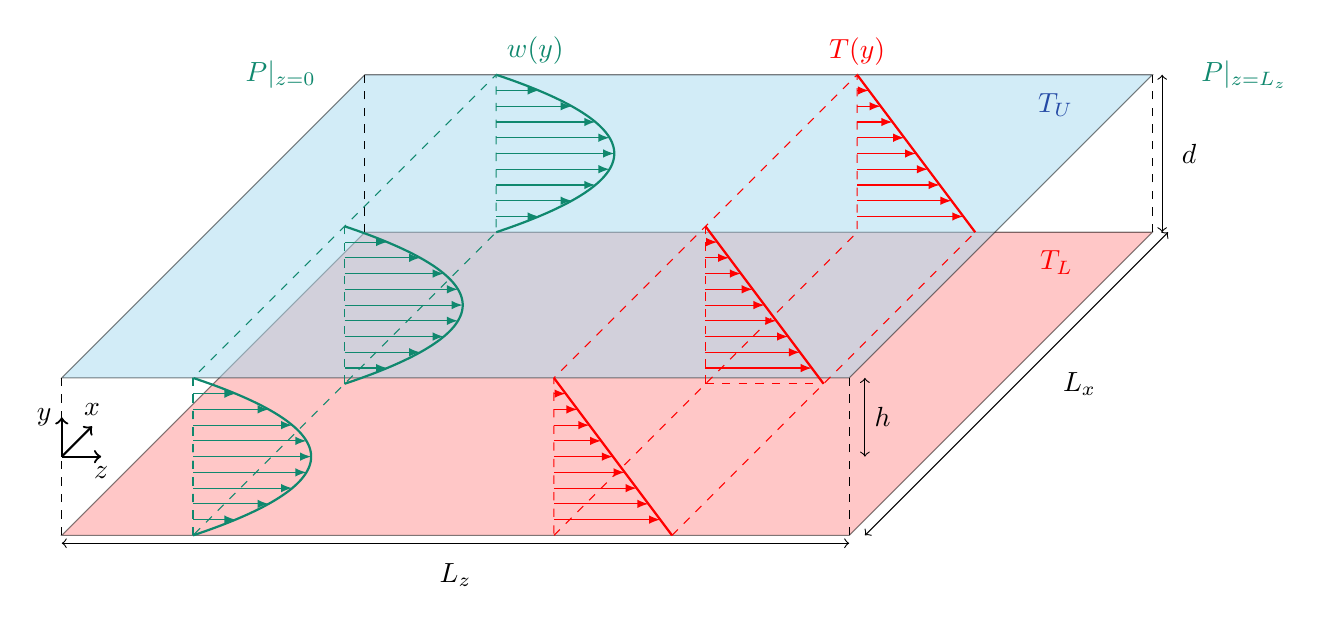
\begin{tikzpicture}
\def\H{1}
\def\W{10}
\def\L{10}

% Draw the bottom plate
\draw [fill=pink!75!red, opacity=0.5] (-\L/2,-\H,0) -- (\L/2,-\H,0) -- (\L/2, -\H, -\W) -- (-\L/2, -\H,-\W) -- cycle;

% Draw the top plate
\draw [fill=SkyBlue!75!white, opacity=0.5] (-\L/2,\H,0) -- (\L/2,\H,0) -- (\L/2, \H, -\W) -- (-\L/2,\H,-\W) -- cycle;

%  % Draw axes
\draw [dashed, thin] (-\L/2, -\H, 0) -- (-\L/2, \H, 0);
\draw [dashed, thin] (\L/2, -\H, 0) -- (\L/2, \H, 0);
\draw [dashed, thin] (\L/2, -\H, -\W) -- (\L/2, \H, -\W);
\draw [dashed, thin] (-\L/2, -\H, -\W) -- (-\L/2, \H, -\W);
%\draw [dashed, thin] (-1,0, 0) --++ (\L,0,0) --++ (0,0,-\W) --++ (-\L,0,0) -- cycle;
%  % \draw [thin, dashed] (-1,0) -- (6,0);

% Add dimensions
% L_x
\draw [<->] (-\L/2,-1.1*\H, 0) -- (\L/2,-1.1*\H,0);
\node[centered] at (0,-1.5*\H,0) {$L_z$};
 
% L_z
\draw [<->] (\L/2*1.025, -\H, -\W) -- (\L/2*1.025, \H,-\W);
\node[right] at (\L/2*1.05,0.0,-\W) {$d$};

% d
\draw [<->] (\L/2*1.04, -\H) -- (\L/2*1.04,-\H,-\W);
\node[centered] at (\L/2*1.2,-\H,-\W/2) {$L_x$};

% h
\draw [<->] (\L/2*1.04, 0, 0) -- (\L/2*1.04, \H, 0);
\node[right] at (\L/2*1.04,\H/2,0) {$h$};

% P
\node[left] at (-\L/2*1.1, \H, -\W) {\textcolor{PineGreen}{$P|_{z=0}$}};
\node[right] at (\L/2*1.1, \H, -\W) {\textcolor{PineGreen}{$P|_{z=L_z}$}};

% T
\node[left] at (\L/2*0.9, \H, -\W*0.9) {\textcolor{cyan!20!blue}{$T_U$}};
\node[left] at (\L/2*0.9, -\H, -\W*0.9) {\textcolor{red}{$T_L$}};

% Draw labels
\draw[->, thick] (-\L/2, 0, 0) -- (-\L/2,\H/2,0) node[left] {$y$};
\draw[->, thick] (-\L/2, 0, 0) -- (-\L/2+\H/2,0,0) node [below] {$z$};
\draw[->, thick] (-\L/2, 0, 0) -- (-\L/2,0,-\H) node[above] {$x$};

% Draw the velocity profile
\draw[PineGreen,thick,domain=-1:1,samples=200,smooth] plot ({(1-\x*\x)*1.5-\L/3}, \x) node[above right] {};
\draw[PineGreen,thick,domain=-1:1,samples=200,smooth] plot ({(1-\x*\x)*1.5-\L/3}, \x, -\W/2) node[above right] {};
\draw[PineGreen,thick,domain=-1:1,samples=200,smooth] plot ({(1-\x*\x)*1.5-\L/3}, \x, -\W) node[above right] {$w(y)$};
\draw[-,PineGreen,dashed] (-\L/3,-\H) -- (-\L/3,\H);
\draw[-,PineGreen,dashed] (-\L/3,-\H, -\W/2) -- (-\L/3,\H, -\W/2);
\draw[-,PineGreen,dashed] (-\L/3,-\H,0) -- (-\L/3,\H,0) -- (-\L/3,\H,-\W) -- (-\L/3,-\H,-\W) -- cycle;

\foreach \y in {-0.8,-0.6,...,0.8} {
    \draw[-latex,PineGreen] (-\L/3,\y, 0) -- ({(1-\y*\y)*1.5-\L/3},\y,0);
    \draw[-latex,PineGreen] (-\L/3,\y, -\W/2) -- ({(1-\y*\y)*1.5-\L/3},\y, -\W/2);
    \draw[-latex,PineGreen] (-\L/3,\y, -\W) -- ({(1-\y*\y)*1.5-\L/3},\y,-\W);
}

% Draw the temperature profile
\draw[red,thick,domain=-\H:\H,samples=200,smooth] plot ({(1/2*(1-\x)*1.5+\L/8)}, \x);
\draw[red,thick,domain=-\H:\H,samples=200,smooth] plot ({(1/2*(1-\x)*1.5+\L/8)}, \x, -\W/2);
\draw[red,thick,domain=-\H:\H,samples=200,smooth] plot ({(1/2*(1-\x)*1.5+\L/8)}, \x, -\W);
\draw[-,red,dashed] (\L/8,-\H,-\W/2) -- (\L/8,\H,-\W/2);
\draw[-,red,dashed] (\L/8,-\H,-\W/2) -- (\L/8 + 1.5,-\H,-\W/2);
\draw[-,red,dashed] (\L/8 +1.5,-\H,0) -- (\L/8 + 1.5,-\H,-\W);
\draw[-,red,dashed] (\L/8,-\H,0) -- (\L/8,-\H,-\W) -- (\L/8,\H, -\W) -- (\L/8,\H,0) -- cycle;
% % 
\foreach \y in {-0.8,-0.6,...,0.8} {
   \draw[-latex,red] (\L/8,\y) -- ({\L/8+(1/2*(1-\y)*1.5},\y);
   \draw[-latex,red] (\L/8,\y, -\W/2) -- ({\L/8+(1/2*(1-\y)*1.5},\y, -\W/2);
   \draw[-latex,red] (\L/8,\y, -\W) -- ({\L/8+(1/2*(1-\y)*1.5},\y, -\W);
}
% Add labels
\node[above,red] at (\L/8,1,-\W) {$T(y)$};
\end{tikzpicture}
\label{fig:rbpconfiguration}
\caption{The Rayleigh-B\'{e}nard Poiseuille (RBP) flow configuration.}
\end{figure}


The RBP configuration is illustrated in figure \ref{fig:rbpconfiguration}, where $z^*, y^*, x^*, L_z, L_x, d, h$ refer to the streamwise, spanwise, wall-normal coordinates, length, span, depth and half-height of the domain respectively.
We note that the asterisks$^*$, refer to variables in dimensional form.
The flow is driven by a pressure gradient along the streamwise $z^*$ direction, $\Delta P^* = P^*|_{z^*=0} - P^*|_{z^*=L_z} < 0$, leading to the formation of a laminar Poiseuille flow, $w^*(y^*)$, for a sufficiently small $\Delta P$. 
In this study, we will only consider fully-developed flow, where the boundary layer from the top and the bottom wall meets at the midplane, $y^*=0$, and entrance effects are neglected.
The RBP configuration is also unstably stratified, such that the temperature difference between the lower, $T_L$, and upper wall, $T_U$, is always positive, $\Delta T = T_L - T_U > 0$, leading to a stable linear conduction profile along the wall-normal direction, $T(y^*)$, if $\Delta T$ is kept sufficiently small.

In the absence of a pressure gradient, the RBP configuration reduces to the classical Rayleigh-B\'{e}nard convection problem, bringing about buoyany-driven convection for a sufficiently large unstable stratification.
In the limiting case without unstable stratification, $\Delta T = 0$, the system reduces to the wall-bounded plane Poiseuille flow (PPF), where the transition towards subscritical shear-driven turbulence may be expected for a sufficiently large pressure gradient.

For instance, do buoyancy forces promote the transition to shear-driven turbulence and how does shear influence the convection? 
To describe the motion of the fluid in RBP configurations, we cosider non-dimensionalised Navier-Stokes equations with Boussinessq approximations,
\begin{subequations}\label{eq:rbp_equations}
\begin{equation}
    \frac{\partial \mathbf{u}}{\partial t} + (\mathbf{u}\cdot\nabla)\mathbf{u} = -\nabla p + \frac{1}{Re}\nabla^2 \mathbf{u} + \frac{Ra}{Re^2Pr} \theta,
\end{equation}
\begin{equation}
    \frac{\partial \theta}{\partial t} + (\mathbf{u} \cdot \nabla)\theta = \frac{1}{RePr}\nabla^2 \theta,
\end{equation}
\begin{equation}
    \nabla \cdot \mathbf{u} = 0.
\end{equation}
\end{subequations}
where $\mathbf{u}(\mathbf{x}), \theta(\mathbf{x}), p(\mathbf{x})$ refers to the nondimensionalised velocity, temperature and presure respectively.
The key control parameters for RBP flows are the Rayleigh number, $Ra$, Reynolds number, $Re$, Prandlt number $Pr$, which are defined as follows,
\begin{equation}
    Ra = \eta g d^3 \Delta T / \nu \kappa, \quad Re = W_c h / \nu, \quad Pr = \kappa / \nu, \quad \Gamma = L/2d,
\end{equation}
where $\eta, g, \Delta T, \nu, \kappa, W_c, h, d, L$ are the thermal expansion coefficient, acceleration due to gravity, temperature difference between the bottom and top wall, kinematic viscosity, thermal diffusivity, laminar centreline velocity, domain's half-depth, full-depth, length or span respectively.

We describe important historical of hydrodynamic stability of planar shear flows and their theorectical frameworks in \S \ref{sec:bkgrd_transitional}.
Theorectical frameworks used in the study of stability of flow such as linear stability, nonlinear dynamical systems and spatiotemporal character of transitional shear flows will be outlined.
This followed the historical developments of Rayleigh-B\'{e}nard convection (RBC), where concepts of the stability of fluid flows will be ultilised in \S \ref{sec:bkgrd_RBC}.
After which, we describe the historical developments of RBP flows \S \ref{sec:bkgrd_RBP}, and the outline of the thesis will be give in \S \ref{sec:thesis_outline}.


% We first discuss the key developments of plane Poiseuille flow (PPF) outlining the key theoretical framework for analysing the stability of fluid flows. This is then followed by Rayleigh-B\'{e}nard convection (RBC) in \S \ref{sec:bkgrd_RBC}.

%%%%%%%%%%%%%%%%%%%%%%%%
% Plane Poiseuille Flows
%%%%%%%%%%%%%%%%%%%%%%%%

\section{Transitional wall-bounded shear flows}\label{sec:bkgrd_transitional}
Wall-bounded shear flows concerns the motion of the fluid flowing in parallel to walls, typically bounded by one or more walls.
The fluid closest to the wall comes to a rest, satisfying the no-slip boundary condition in the presence of a wall.
As a consequence, a velocity gradient in the direction perpendicular from the wall develops, where the fluid layer becomes \emph{sheared} due to the pressence of the wall - referred to wall-bounded sheared flows.
% In Newtonian fluids, shear stresses are directly proportionate to the velocity gradient by the fluids kinetic viscosity, $\nu$, given as,
% \begin{equation}\label{eq:shear}
%    \tau = \nu \frac{\partial u}{\partial y},
% \end{equation}
% where $\tau$, $\nu$, and $\frac{\partial u}{\partial y}$ refers to shear stresses - hence wall-bounded shear flows.
Example of wall-bounded shear flows include the pressure-driven plane Poiseuille flow (or channel flow), Hagen-Poiseuille (or pipe) flows, plane Couette flow and flat plate boundary layers.
These geometrically simple examples enables a convenient framework amenable to the mathematical analysis of fluid motion subjected to shear.
Depending on the degree of shear, the fluid motion can be either laminar, where the fluid layers move in smooth parallel 'laminates', or turbulent, characterised by chaotic eddying motions.
We also note that there is a transitional regime where both states can coexist discuss later.
A central question is predicting the transition from the laminar regime to the turbulence.
% One of the central questions is on the prediction on the transition to turbulence, specifically, when is turbulence expected as shear is increased?
% plane Poiseuille flow (PPF) describes the motion of a fluid confined between two infinitely extended parallel walls, driven by a pressure gradient, also referred to as channel flow.
% It belongs to a general class of wall-bounded shear flows, consisting of plane Couette flow, pipe (Hagen-Poiseuille) flow and flat plate boundary layer flow.

The earliest investigation into this transition dates back to the pipe flow experiments of \cite{reynolds_xxix_1883}.
In his experimental setup, the flow speed through the pipe could be controlled by regulating the inlet pressure, while injecting dye to visualise the flow, as illustrated in figure \ref{fig:reynolds}(a).
At low speeds, the fluid remained laminar, resulting to a single streak of steady dye in figure \ref{fig:reynolds}(b).
As the speed increased, the dye begin to exhibit irregular `sinuous' motions interspersed with laminar regions shown in figure \ref{fig:reynolds}(c).
This is now referred to as the transitional/intermittent regime, alternating between the laminar and turbulent states.
Beyond a critical speed, the dye breaks down entirely into chaotic `eddies', mixing with the surrounding fluid and discolouring the flow with dye downstream in figure \ref{fig:reynolds}(d).
This regime is now identified as turbulence.

Reynolds conjectured that the threshold between the laminar, transitional and turbulent regimes could be characterised by the Reynolds number, $Re = U D/\nu$, where $U$ is the centerline velocity in the pipe, $D$, the pipe diameter and $\nu$, the kinematic viscosity.
He observed that flow through the pipe remained `stable' and laminar for $Re < 1900$, while it became `unstable' and turbulent for $Re > 2000$ \citep{reynolds_iv_1895}.
His remarks led to the concept of the stability of fluid flows.
\begin{figure}[h]
    \centering
    \includegraphics[width=1\textwidth]{Background/Figures/Reynolds.pdf}
    \caption{(a) Osbourne Reynolds pipe experiment with the dye injection apparatus, illustrating the (b) laminar flow, (c) intermittent regime and (d) turbulent flow as the flow speed is increased, taken from \citep{reynolds_xxix_1883}.}
    \label{fig:reynolds}
\end{figure}

%%%%%%%%%%%%%%%%%%%%%%%%%%%
% Linear Stability Analysis
%%%%%%%%%%%%%%%%%%%%%%%%%%%

\subsection{Linear Stability Analysis}
Following Reynolds' experiment, interest towards the mathematical analysis of the stability of fluid flows grew in early $20^{st}$ century.
The mathematical approach typically begins by decomposing the velocity field, $\mathbf{u}(\mathbf{x},t)$, into a laminar (base) state, $U(y)$ (assumed to depend only on the wall-normal direction here), and the velocity perturbations, $\mathbf{u}'(\mathbf{x},t)$, with pressure similarly decomposed as,
\begin{equation}
    \mathbf{u}(\mathbf{x}) = U(y) + \mathbf{u}'(\mathbf{x},t), \quad \text{and} \quad p(\mathbf{x},t) = P(x) + p'(\mathbf{x},t).
\end{equation}
Next, we the substitute the formulations for the decomposed velocity and pressure into the Navier-Stokes equations of equation \eqref{eq:rbp_equations} and drop the nonlinear pertubrations terms $(\mathbf{u'}\cdot \nabla)\mathbf{u'}$,
\begin{subequations}\label{eq:shear_linearised}
\begin{equation}
    \frac{\partial \mathbf{u'}}{\partial t} + (U \cdot\nabla)\mathbf{u'} + (\mathbf{u'}\cdot\nabla)U= -\nabla p' + \frac{1}{Re}\nabla^2 \mathbf{u'},
\end{equation}
\begin{equation}
    \nabla \cdot \mathbf{u}' = 0,
\end{equation}
\end{subequations}
resulting to the linearised Navier-Stokes equations. 
This commonly followed by introducing a wavelike ansatz (mode) defined by streamwise and spanwise wavenumbers, $\alpha, \beta$ and complex frequency, $\omega$.
In general two ways to analysis the linearised Navier-Stokes equations by considering the behaviour of each mode independently in \S \ref{subsec:modal} and their coupled dynamics in \S \ref{subsec:nonmodal}

%%%%%%%%%%%%%%%%%
% MODAL STABILITy
%%%%%%%%%%%%%%%%%

\subsubsection{Modal analysis}\label{subsec:modal}
It is covenient to eliminate the pressure terms by to transform equation \eqref{eq:shear_linearised} using the wall-normal perturbation velocity, $v'$, and wall-normal vorticity, $\eta' = \partial u'/ \partial z - \partial w' / \partial x$, variables.
Using $(v, \eta)$, introduce an ansatz (mode) for them,
\begin{equation}\label{eq:shear_ansatz}
    v'(\mathbf{x},t ) = \tilde{v}(y)e^{i(\alpha x + \beta z - \omega t)}, \quad \text{and} \quad \eta'(\mathbf{x}, t) = \tilde{\eta}(y)e^{i(\alpha x + \beta z - \omega t)}.
\end{equation}
where $\alpha, \beta, \omega$ denotes the streamwise and spanwise wavenumbers, and complex frequency (i.e. $\omega = \omega_r + i\omega_i$), respectively.
Next, we substitute the ansatz into equation \ref{eq:shear_linearised}, leading to the classical Orr-Sommerfeld and Squire equations \citep{orr_stability_1907,sommerfeld_beitrag_1909,squire_stability_1933, schmid_stability_2001},
\begin{equation}\label{eq:OSQ}
    \left[
    -i\omega 
    \begin{pmatrix}
        k^2 - \mathcal{D}^2 & 0 \\
        0 & 1 
    \end{pmatrix}
    + 
    \begin{pmatrix}
        \mathcal{L}_{OS} & 0 \\
        i\beta U' & \mathcal{L}_{SQ} 
    \end{pmatrix}
\right ]
    \begin{pmatrix}
        \tilde{v} \\
        \tilde{\eta}
    \end{pmatrix}
    = \mathbf{0},
\end{equation}
where $\mathcal{L}_{OS}$ and $\mathcal{L}_{SQ}$ refers to the Orr-Sommerfeld and Squire operators given as,
\begin{subequations}
  \begin{equation} 
      \mathcal{L}_{OS} = i\alpha U(k^2-\mathcal{D}^2) + i\alpha U'' + \frac{1}{Re}(k^2 - \mathcal{D}^2)^2,
  \end{equation}
  \begin{equation} 
      \mathcal{L}_{SQ} = i\alpha U + \frac{1}{Re}(k^2 - \mathcal{D}^2).
  \end{equation}
\end{subequations}
$k^2, \mathcal{D}, U', U''$ denotes the sum of squared wavenumbers, $k^2 = \alpha^2 + \beta^2$, differential operator in $y$, first- and second- derivative of the laminar velocity, respectively.
Equation \eqref{eq:OSQ} is simply an eigenvalue problem which could be represented as,
\begin{equation}
    \mathbf{L}\mathbf{\tilde{q}} = i\omega\mathbf{M}\mathbf{\tilde{q}}
\end{equation}
    where,
\begin{equation}
    \mathbf{L} = \begin{pmatrix}
        \mathbf{L}_{OS} & 0 \\
        i\beta U' & \mathcal{L}_{SQ}
    \end{pmatrix},
    \quad \mathbf{M}
    \begin{pmatrix}
        k^2 - \mathcal{D}^2 & 0 \\
        0 & 1 
    \end{pmatrix}, 
    \quad \mathbf{\tilde{q}} = 
    \begin{pmatrix}
        \tilde{v} \\
        \tilde{\eta}
    \end{pmatrix}.
\end{equation}
and $i \omega$ refers to the eigenvalue.
The aim of linear stability analysis is to determine the critical Reynolds number, $Re_c$, which is defined as the lowest value of $Re$ over $\alpha$ and $\beta$, such that $Im[\omega] = 0$.
For $Re > Re_c$, perturbations could grow exponentially, departing from the laminar state.
In other words, we consider the behaviour of each $\alpha-\beta$ mode independently, herein referred to as \emph{modal} analysis.
Squire's theorem implies that for any unstable three-dimensional perturbations, $\beta \neq 0$, there exist an unstable two-dimensional perturbation, $\beta = 0$ with a lower $Re_c$ \citep{squire_stability_1933}.
Therefore, the unstable perturbations of wall-bounded shear flows at $Re_c$ must be two-dimensional.
The theoretical calculations was first perform by \cite{tollmien_uber_1928} and \cite{schlichting_zur_1933} for a flat-plate boundary layer flow, yielding a critical Reynolds number based on streamwise distance $x$ of $Re_{x,c} = Ux_c / \nu = 520$ \citep{schlichting_onset_2017}.
In their honour, the unstable two-dimensional perturbations of the Orr-Sommerfeld operator is referred to as Tollmien-Schlicting (T.S) waves.
For plane Poiseuille flow \citep{orszag_accurate_1971} with a critical wavenumber of $\alpha_c = 1.02$.
However, turbulence in plane Poiseuille flows have been observed at much lower Reynolds number, $Re \sim 1000 - 2000$, contradicting the results from linear stability analysis.
Likewise, the onset of turbulence appear near $Re_{x,c} \approx 5 \times 10^5$ for flat plat boundary layer.
% The aim of linear stability analysis it to search for eigenvalues across $\alpha, \beta, Re$, such that $w_i \geq 0$, denoting an exponential growth of perturbations above a critical Reynolds number defined as $Re_c= \min(\alpha, \beta, Re)|_{\omega = 0}$.
% Interestingly, linear stability analysis for pipe flow predicts a stable laminar flow for all Reynolds numbers \citep{romanov_stability_1973}, contradicting experiments \citep{reynolds_xxix_1883,avila_onset_2011}.
A similar result holds for the plane Couette flow \citep{meseguer_linearized_2003}.
% The critical Reynolds number for the onset of unstable infinitesimal perturbutations in plane Poiseuille flow (PPF) occurs at $Re_{c} = 5772.2$ \citep{orszag_accurate_1971}.
Despite its limitation, linear analysis analysis succeeds in predicting the critical Rayleigh number in Rayleigh-B\'{e}nard convection.
% Despite it failures, it has succeeded in other configurations, such as Rayleigh-B\'{e}nard convection, and Taylor-Couette flow \citep{bodenschatz_recent_2000}, predicting the onset of convection and Taylor rolls are the correct critical parameters.

%%%%%%%%%%%%%%%%%%%%%
% Non-modal stability
%%%%%%%%%%%%%%%%%%%%%

\subsubsection{Non-modal stability}\label{subsec:nonmodal}
One of a major limitation of linear stability analysis considered above is that it treats each eigenmode independently, referred to as \emph{modal} analysis.
However, the interaction between decaying eigenmodes may lead to a short-term amplification of perturbations, before eventually decaying.
This phenonemon is referred to as \emph{transient growth}, and the method of analysis is referred to as \emph{non-modal} analysis, related to the normality of the linear Orr-Sommerfeld operator \citep{schmid_nonmodal_2007}.
\begin{figure}[h]
    \centering
    \includegraphics[width=\textwidth]{Background/Figures/PhasePotrait.pdf}
    \caption{(a) The phase portrait of the toy model with $Re = 15$, (b) Transient growth.}
    \label{fig:toy_model}
\end{figure}
To demonstrate an example of transient growth, we consider a two-dimensional toy model governing the time-evolution of $\mathbf{q}$,
\begin{equation}
    \frac{\mathrm{d}}{\mathrm{d}t} \begin{pmatrix} v \\ \eta \end{pmatrix}  = \begin{pmatrix} -\frac{1}{Re} & -1 \\ 0 & -\frac{2}{Re} \end{pmatrix} \begin{pmatrix} v \\ \eta \end{pmatrix},
\end{equation}
where $Re$ refers to the Reynolds number.
The toy model is has negative eigenvalues, $(\lambda_1, \lambda_2) = (-1/Re, -2/Re)$, and unit eigenvectors $\mathbf{x_1} = (1, 0)$, $\mathbf{x_2} = \frac{1}{\sqrt{Re^2 + 1}}(Re, 1)$.
Judging from the negative eigenvalues, we conclude that $\mathbf{q}(t)$ will decay exponentially.
However, as $Re \rightarrow \infty$, they becoming increasingly non-orthogonal approaching each other such that the angle between $\mathbf{x}_1$ and $\mathbf{x}_2$ tend towards 0.
At $Re = 15$, the eigenvector pairs, $\mathbf{x_1}$ and $\mathbf{x_2}$, are highly non-orthogonal, becoming almost linear dependent shown in figure \ref{fig:toy_model}(a).
For a randomly selected initial condition with an energy-norm of $||\mathbf{q}_0||_2 = 15$, where $|| \cdot ||_2$ refers to the L2-norm, the trajectory in green decays exponentially for $t \in [0, 100]$ in figure \ref{fig:toy_model}(b).
In constrast, for a specifically chosen initial condition in shown as the blue trajectory, $||\mathbf{q}||_2$ is amplified nearly four times before decaying exponentially.
The toy model demonstrates the significance of transient growth for a specifically chosen initial condition.

The goal of non-modal stability analysis is to searching over all initial conditions, $\mathbf{\tilde{q}}_0$, leading to the maximum amplification factor at time $t$, resulting in an optimisation problem,
\begin{equation}\label{eq:transient_growth}
    % G(t) = \max_{\mathbf{\tilde{q}}_0 \neq 0 } \frac{||\mathbf{\tilde{q}}(t)||^2}{||\mathbf{\tilde{q}}_0||^2}, \quad \text{s.t} \quad ||\mathbf{\tilde{q}}_0||^2 = 1,
    G(t) = \max_{\mathbf{\tilde{q}}_0 \neq 0 } \frac{\langle \mathbf{\tilde{q}}(t), \mathbf{\tilde{q}}(t) \rangle }{\langle \mathbf{\tilde{q}}_0, \mathbf{\tilde{q}}_0 \rangle }, \quad \text{s.t} \quad \langle \mathbf{\tilde{q}}_0, \mathbf{\tilde{q}}_0 \rangle = 1,
\end{equation}
where, $\langle \cdot, \cdot \rangle$ refers to the inner-product defined as,
\begin{equation}
    \langle \mathbf{x}, \mathbf{y} \rangle = \int_\Omega \mathbf{x}^H \mathbf{y} \; \mathrm{d}\Omega,
\end{equation}
and $\mathbf{x}^ H$ refers to the complex conjugate transpose of $\mathbf{x}$.
By considering the linearised operator of \eqref{eq:OSQ}, we can define a linear time invariant operator given as,
\begin{equation}\label{eq:linear_evolution}
    \mathbf{\tilde{q}}(t) = \mathcal{A}(t) \mathbf{\tilde{q}}_0,
\end{equation}
which takes the solution from initial conditions, $\mathbf{\tilde{q}}_0$, to $\mathbf{\tilde{q}}(t)$ at time $t$.
Subtituting the expression above into equation \eqref{eq:transient_growth},
\begin{equation}\label{eq:transient_growth_adj}
    G(t) = \max_{\mathbf{\tilde{q}}_0 \neq 0 } \frac{\langle \mathcal{A}(t)\mathbf{\tilde{q}}_0, \mathcal{A}(t)\mathbf{\tilde{q}}_0 \rangle }{\langle \mathbf{\tilde{q}}_0, \mathbf{\tilde{q}}_0 \rangle} = \langle \mathbf{\tilde{q}}_0, \mathcal{A}^\dagger(t) \mathcal{A}(t)\mathbf{\tilde{q}}_0  \rangle = \lambda_{max} (\mathcal{A}^\dagger \mathcal{A})
\end{equation}
where $\mathcal{A}^\dagger(t)$ refers to the adjoint of $\mathcal{A}(t)$. The maximum amplification factor $\max G(t)$ is the largest eigenvalue, $\lambda_{max}$, of $\mathcal{A}^\dagger \mathcal{A}$, and the eigenvalue problem is given as,
\begin{equation}
    \mathcal{A}^\dagger(t)\mathcal{A}(t) \mathbf{\tilde{q}}_0 = \lambda \mathbf{\tilde{q}}_0,
\end{equation}
where $\mathbf{\tilde{q}}_0$ refers to the eigenvector denoting the optimal initial condition.
For a detailed derivation of the optimal initial conditions or forcing, the reader is referred to \citep{butler_three-dimensional_1992,schmid_nonmodal_2007}.
An alternative method of computing transient growth is computing the pseudospectral of linear operators discussed in \citep{trefethen_pseudospectra_1997}, outside the scope of this thesis.

Both two-dimensional, $\beta = 0$, and three-dimensional, $\beta \neq 0$, non-modal stability analysis have been studied.

In the two-dimensional form, the optimal initial conditions are in the form of near wall vorticies tilted upstream, transiently energised referred to as the Orr-mechanism \citep{orr_stability_1907, farrell_optimal_1988,reddy_pseudospectra_1993}.
In the three-dimension form, streamwise vortices, acting as optimal initial conditions lead to the optimal response in the form of streamwise streaks \citep{reddy_energy_1993}.
Contrary to linear stability analysis which confers two-dimensional perturbations as linearly unstable, the key result in this analysis is that three-dimensional initial conditions, $\alpha = 0$, confer the optimal initial conditions leading to large transient growth at subcritical Reynolds numbers.
Figure.. shows this.

The width of the streaks happen to be robustly occur around 100 wall units, the characteristics spacing identified in many experiments [Kline, Panton, Bandybopobi]

The optimal initial conditions involve streamwise vortices which amplify streaks, related to the lift-up effect \citep{ellingsen_stability_1975,brandt_lift-up_2014}.
These modal and nonmodal mechanisms above highlight developments based on linear methods.

% \begin{equation}
%     \langle \mathcal{A}(\tau)\mathbf{x}, \mathbf{y} \rangle = \langle \mathbf{x}, \mathcal{A}^\dagger(\tau) \mathbf{y} \rangle.
% \end{equation}
% Next, we convert the constraint optimisation \eqref{eq:linear_growth_adj} into an unconstraint Lagrangian using Lagrange multipliers,
% \begin{equation}
%     \mathcal{L} = \langle \mathbf{\tilde{q}}_0, \mathcal{A}^\dagger\mathcal{A}\mathbf{\tilde{q}}_0 \rangle  + \lambda (\langle \mathbf{\tilde{q}}_0, \mathbf{\tilde{q}}_0 \rangle - 1)
% \end{equation}
% \begin{equation}
%     \delta L / \delta \mathbf{\tilde{q}}_0 = 2 \mathcal{A}^\dagger\mathcal{A}\mathbf{\tilde{q}}_0 - 2\lambda \mathbf{\tilde{q}}_0 = 0,
% \end{equation}
% where $\lambda$ refers to the Lagrange multiply.
% By invoking the optimal conditions, $\delta L/ \delta \mathbf{\tilde{q}}_0 = 0$, we get,
% \begin{equation}
%     \mathcal{A}^\dagger\mathcal{A}\mathbf{\tilde{q}}_0 = \lambda \mathbf{\tilde{q}},
% \end{equation}

% The maximum amplification factor $G(\tau)$ is simply the maximum eigenvalue of $\mathcal{A}^\dagger(\tau) \mathcal{A}(\tau)$, expressed as,
% Next, we describe the transient approach for Orr-Sommerfeld problem, by first casting it in its time-evolution form,
% \begin{equation}
%     \frac{\partial}{\partial t} \mathbf{\tilde{q}} = 
%     \begin{pmatrix}
%         (D^2 - k^2)^{-1}\mathcal{L}_{OS} & 0 \\
%         -i\beta U' & -\mathcal{L}_{SQ}
%     \end{pmatrix}
%     \mathbf{\tilde{q}},
% \end{equation}
% Next, we consider the evolution equations of the Orr-Sommerfeld operator as,
% where the solution at time $\tau$ is given as,
% \begin{equation}
%     \mathbf{\tilde{q}}(\tau) = \exp(\mathcal{A}\tau) \mathbf{\tilde{q}}_0
% \end{equation}
% where $\mathbf{A} \mathbf{V}= \mathbf{V}\mathbf{D}$ is diagonalisable where $\mathbf{V}, \mathbf{D}$ refer to the eigenvectors and values respectively.
% 
% \begin{equation}
%     G(t) = \max_{\mathbf{\tilde{q}_0} \neq 0} \frac{||\mathbf{\tilde{q}}(t)||^2}{||\mathbf{\tilde{q}}_0||^2}, \quad \text{s.t} \quad ||\mathbf{\tilde{q}_0}||^2 = 1.
% \end{equation}
% The energy-norm is defined with a continuous inner-product,
% \begin{equation}
%     ||\mathbf{x}
% \end{equation}
% \begin{equation}
%     ||\mathbf{\tilde{q}}(t)||^2 = \langle \mathbf{A}(t) \mathbf{\tilde{q}_0}, \mathbf{A}(t) \mathbf{\tilde{q}_0} \rangle = \int_\Omega (\mathbf{A}\mathbf{\tilde{q}})^* \mathbf{A}\mathbf{\tilde{q}} \; \mathrm{d} \Omega,
% \end{equation}
% where $\cdot^{*}$ refer to the complex conjugate.
% Next, we introduce the adjoint operator where,
% \begin{equation}
%     \langle \mathbf{x}^\dagger, A x \rangle = \langle A^\dagger \mathbf{x}, \mathbf{x} \rangle
% \end{equation}
% \begin{equation}
%     G(t) = \max_{\mathbf{\tilde{q}_0} \neq 0} \frac{||\mathbf{\tilde{q}}(t)||^2}{||\mathbf{\tilde{q}}_0||^2} = \max_{\mathbf{\tilde{q}_0} \neq 0} \frac{\mathbf{a_0}^T\exp(\mathbf{D}t)\mathbf{V}^T\mathbf{V}\exp(\mathbf{D}t)\mathbf{a}_0}{\mathbf{a}_0^T \mathbf{V}^T \mathbf{V} \mathbf{a}_0}
% \end{equation}
% \begin{equation}
%     G(t) = \max_{\mathbf{\tilde{q}_0} \neq 0} \frac{||\mathbf{\tilde{q}}(t)||^2}{||\mathbf{\tilde{q}}_0||^2} = \max_{\mathbf{\tilde{q}_0}} \frac{\mathbf{\tilde{q}_0}^T \mathbf{A}^T \mathbf{A} \mathbf{\tilde{q_0}}}{\mathbf{q}_0^T\mathbf{q}_0}
% \end{equation}
%%%%%%%%%%%%%%%%%%%%%%%%%%%%%
% NONLINEAR DYNAMICAL SYSTEMS
%%%%%%%%%%%%%%%%%%%%%%%%%%%%%

\subsection{Nonlinear dynamical systems}

\begin{figure}[h]
    \centering
    \includegraphics[width=0.8\textwidth]{Background/Figures/StateSpaceGraham.png}
    \caption{The state space organising of the upper and lower branch. Turbulence is interpreted as solution trajectories wander around the upper branch, orbiting around a network unstable invariant states. The lower branch acts as a boundary between the turbulent attractor and laminar attractor, an attracttor on the edge referred to as the edge state. Taken from \citep{graham_exact_2021}.}
    \label{fig:StateSpaceGraham}
\end{figure}

In the previous section, we have examined the transition process based linear mechanisms.
Unfortunately, for canonical shear flow configurations, the transition process is subscritical where linear stability theory fails to predict the onset of turbulence.
Furthermore, the transition to turbulence is ultimately governed fully nonlinear nature of the Navier-Stokes equations.
Hence, we turn to a nonlinear dynamical systems point of view of this transition process, inspired from Hopf's vision of transition, where turbulence emerge as a chaotic trajectory after succeeding Hopf bifurcations.. [CHECK THIS DESCRIPTION...]
However, this bifurcation cannot happen in the subcritical 
In this view, turbulence is interpreted as a solution trajectory evolving through a phase space composed of a network such non-trivial nonlinear solutions, commonly referred to as exact coherent states (ECS) or invariant solutions \citep{graham_exact_2021}.

In the context of parallel shear flows, Nagata was the first to discover a pair of unstable equilibirum solutions in plane Couette flow by smoothly following (homotopy) from a Taylor-Couette configuration \citep{nagata_three-dimensional_1990}.
This pair consist of an unstable upper branch and lower branch emerging as a saddle-node bifurcation near $Re \approx 500$, and is disconnected from the stable laminar solution.
The lower branch refers to its proximity towards the stable laminar state in phase space.
A travelling-wave solution in plane Couette flow also later found by the same author \citep{nagata_three-dimensional_1997}.
A family of equilibrium and travelling waves solutions was found for plane Couette and plane Poiseuille flows under various boundary conditions (i.e. stress-free, slip and no-slip) where identified by \citep{waleffe_exact_2001,waleffe_homotopy_2003}.

While these unstable solutions demonstrate good agreements with results from DNS such as the spanwise length scales, and mean and fluctuations, they do not capture the dynamical processes.
Periodic orbits defined by time-dependent solutions that have been identified in plane Couette flow \citep{kawahara_periodic_2001}, describing a single regeneration cycle similar to the self-sustaining process.
The chaotic trajectories of turbulence have been found to be embedded within invariant solutions and their connections between them known as heteroclinic orbits, offering a robust view of the building-blocks of of turbulence \citep{gibson_visualizing_2008, gibson_equilibrium_2009, viswanath_recurrent_2007, halcrow_heteroclinic_2009, graham_exact_2021}

In the context of this transitional flows, the lower branch solution can be though of separating the turbulent attractor from the laminar state.
Its an attractor that resides on the edge of turbulence, defined as an edge state.
The graphical representation of this edge is shown in figure \ref{fig:StateSpaceGraham}.

% Coherent structures and turbulent motions
These invariant solutions commonly take the form of as equilibria, travelling waves, periodic and relative periodic orbits.
It is well established that coherent motions defined by flow patterns that persist in space and time play an important role in the transport of momentum and heat.
In parallel shear flows, these coherent structures typically appear as near-walls streaks and quasi-streamwise rollers.
A persistent, quasi-periodic cycle between the regeneration of streaks and rolls, referred to as the \emph{self-sustaining process}, appears to be a fundamental mechanism in sustaining wall-bounded turbulence \emph{self-sustaining process} \citep{hamilton_regeneration_1995}.
This mechanism is described by the generation of streaks due to quasi-streamwise rollers by redistributing the mean.
These streaks become linearly unstable and breakdown, and through a nonlinear process regenerates the quasi-streamwise rollers, closing the cycle.

% Utilising tools from nonlinear dynamics systems, turbulence could be viewed as chaotic trajectories around unstable nonlinear solutions known as invariant solutions or exact coherent structures \citep{Waleffe_2001,Waleffe_2003,toh2003periodic,Kreilos_2012,nagata2013mirror,Wall_Nagata_2016,Zammert_Eckhardt_2014,graham21}.

%%%%%%%%%%%%%%%%%%%%%%%%%%%%%%%%%%%
% Spatiotemporal transitional flows
%%%%%%%%%%%%%%%%%%%%%%%%%%%%%%%%%%%

\subsection{Spatiotemporal transitonal flows}
\begin{figure}[h]
    \centering
    \includegraphics[width=\textwidth]{Background/Figures/Re1400.pdf}
    \caption{A snapshot of turbulent-laminar bands at $Re = 1400$ in a large domain $L/d = 8\pi$, depecting its spatiotemporal intermittent nature. Isovolume renderings is based on the spanwise, $u'$, and wall-normal, $v'$, perturbation kinetic energy, $E(u',v') = 1/2(u'^2 + v'^2)$, where the perturbation velocities are defined about the laminar state $\mathbf{u}'(\mathbf{x},t) = \mathbf{u}(\mathbf{x},t) - U_{lam}(y)$.}
    \label{fig:turbulent-laminar}
\end{figure}

This section describes the inherent spatiotemporal intermittent description of turbulence in transitional wall-bounded shear flows commonly reported in large extended domains where the span is about fifty times the half-height of a plane Poiseuille channel, $L/h \gtrsim 50$.
In thie regime, turbulence is characterised by the coexistence of turbulent and laminar structures.
Examples of such are found in canonical shear flow systems such as plane Couette flows \citep{prigent_long-wavelength_2003,barkley_computational_2005,barkley_mean_2007,tuckerman_patterns_2011,duguet_formation_2010,reetz_exact_2019}, Taylor-Couette flows \citep{prigent_barber_2002,prigent_long-wavelength_2003}, pipe flows \citep{avila_transient_2010,avila_onset_2011,song_speed_2017,avila_transition_2023} and plane Poiseuille flows \citep{tsukahara_dns_2014, tsukahara_dns_2014-1, tuckerman_turbulent-laminar_2014, tsukahara_experimental_2014, gome_statistical_2020, paranjape_onset_2019, paranjape_oblique_2020, paranjape_direct_2023}.

We will focus on the plane Poiseuille flow configuration, where the spatiotemporal intermittent patterns are referred to as oblique turbulent-laminar bands illustrated in figure \ref{fig:turbulent-laminar} at $Re = 1400$ for $L/h = 16\pi$.
The the bright and dark regions highlights coexisting spatially localised turbulent and laminar regions.
These turbulent-laminar bands occur over a range of Reynolds numbers, and its precise range is likely dependent on the domain's aspect ratio \citep{tsukahara_experimental_2014,tuckerman_turbulent-laminar_2014,paranjape_direct_2023}.
Near the upper $Re$ threshold of this regime, the domain is fully engulfed by developed turbulent regions, referred to uniform, featureless turbulence appearing at $Re = 1800$ in figure \ref{fig:turbulent-laminar}(a).
As $Re$ decreases towards $Re = 1050$, turbulent-laminar bands persist in figures \ref{fig:turb_lam_bands}(b-f).
In this region, turbulent-laminar bands angles have been observed to be inclined between $20^\circ \sim 30^\circ$, with streamwise wavelengths of $\sim 60h$, and spanwise wavelengths of $\sim 20h-30h$ \citep{tsukahara_experimental_2014}.
To study the preference of angles, zzz performed linear stability analysis of bands and showed that preferred angle at .. degrees.
Below certain $Re$ threshold, the spatially turbulent regions spontaneously decay where the flow relaminarises asymptotically \citep{tuckerman_turbulent-laminar_2014}.
This decay is shown in $Re = 1000$ near $t = 1600$ in figure \ref{fig:turb_lam_bands}(g). 
\begin{figure}[h]
    \centering
    \includegraphics[width=\textwidth]{Background/Figures/Ra0-BotSpaceTime.pdf}
    \caption{Turbulent-laminar bands for $t \in [0, 3000]$ in large domains $(L_x, L_z) = (16\pi, 16\pi)$ at (a) $Re = 1800$, (b) $Re = 1600$, (c) $Re = 1400$,  (d)  $Re =1200$, (e) $Re = 1100$, (f) $Re = 1050$,  (g) $Re = 1000$.}
    \label{fig:turb_lam_bands}
\end{figure}

Inspired from previous studies of turbulent-laminar bands in plane Couette flows \citep{barkley_computational_2005, reetz_exact_2019}, narrow domains, titled orthogonally to the band angles where considered to investigate their dynamics \citep{tuckerman_turbulent-laminar_2014, paranjape_oblique_2020, paranjape_direct_2023}.
In narrow-tilted domains inclined at $24^\circ$, the turbulent-bands convect at about $\sim1\%$ of the bulk velocity, propagating either upstream or downstream, above or below an critical $Re \sim 1000$, independent of domain sizes for $L_z \geq 100h$ \citep{tuckerman_turbulent-laminar_2014,gome_statistical_2020}.
\begin{figure}[h]
    \centering
    \includegraphics[width=0.7\textwidth]{Background/Figures/gome_prob.pdf}
    \caption{The mean decay times (red), $\tau^d$, and mean splitting times (black), $\tau^s$, as a function of Reynolds number, leading to a crossover point at $Re \approx 965$, adapted from \citep{gome_statistical_2020}.}
    \label{fig:decay_split_probability}
\end{figure}
The characteristic spanwise wavelengths of turbulent-laminar bands are depdendent on $Re$, appearing at $\lambda_z \sim 20h$ for $Re \geq 1400$ and $\lambda_z \sim 40h$ for $Re \leq 1100$.
Indeed, between $1300 < Re < 1400$ the bands appear to alternative between two different band-widths \citep{tuckerman_turbulent-laminar_2014}, merging and splitting continuously. 
This points towards a band splitting event in between $Re = 1100$ and $Re = 1400$, reminiscent of a puff splitting in pipe flows \citep{avila_onset_2011}.

On the other hand, turbulent bands appear to decay at $Re = 830$ \citep{gome_statistical_2020}, and at $re = 1100$ but surviving for $re = 1000$ \citep{tuckerman_turbulent-laminar_2014}, suggesting that turbulent bands decay spontaneously.
\citep{gome_statistical_2020} computed the probabilities distributions of turbulent band decay, $P(\Delta t^d)$, where $\Delta t^d$ refers to the time it takes for decay.
On of the key insight is that the probability distributions of turbulent band decay mimicks a memoryless Poisson distribution,
\begin{equation}
    P(\Delta t^d) = \exp(-\Delta t^d/\tau^d(Re)),
\end{equation}
where $\tau^d(Re)$ refers to the mean lifetime for decay as a function of $Re$.
Similarly, the probability distribution for band splitting also follows a Poisson distribution, $P(\Delta t^s) = \exp(-\Delta t^s / \tau^s(Re))$, where $\tau^s(Re)$ refers to the mean lifetime of a splitting event dependent on $Re$.
The mean survival lifetime of a band decaying, $\tau^d$, and splitting, $\tau^s$, depends superexponentially on $Re$, i.e. $\tau^{d,s} = \exp(\exp(Re))$.
This superexponential dependence is presented in figure \ref{fig:decay_split_probability}, with a crossover point at $Re_{cross} \approx 965$.
This crossover point refers to equal mean survival lifetime of a band de
suggesting a critical $Re$ for the onset of turbulent bands.
% By extrapolating the estimated mean lifetimes of a splitting and decay event, the crossing point (i.e equal chance of identifying a splitting and decay event after a time-scale of $t = 3 \times 10^6$) occurs at $Re_{cross} \approx 965$, in other words, $Re_{cross}$ acts as a critical Reynolds number.
While there has substantial progress made towards understanding the behaviour of periodic turbulent-laminar bands in narrow-tilted domains, recently studies of isolated turbulent bands (ITBs) indicate differed behaviour.
Notably, ITBs persist at $Re \approx 700$ for $t = 10000$ (far beyond figure \ref{fig:decay_split_probability}, characterised by streak generating head, and a diffusive upstream tail. \citep{xiong_turbulent_2015, tao_extended_2018, shimizu_bifurcations_2019, xiao_growth_2020}.
% It is worth noting that isolated bands are not memoryless, depending on their pass history [citation]
% Above a certain Reynolds number, the probability of band splitting again depends on a super-exponentianal.
% Show graph.
% In the context of plane Poiseuille flowsd, it is well known that at $Re \sim 1000 - 2000$, turbulence behaves intermittently, existing as oblique bands of turbulent and laminar regions. 
% Over the past decade, research efforts have been dedicated to the study of turbulent-laminar bands.

% At $Re \sim 1000 - 2000$, turbulent bands can either decay spontaneously, stabilising into a laminar state, or split, forming more bands whereby turbulent-laminar bands are sustained.
% The probability of decay and splitting lifetimes strongly depends on the domain size and $Re$.
% At $L_z = 100h$, the critical Reynolds number of $Re_{cr} \approx 965$ have been determined statistically, whereby decay and splitting lifetimes intersect more than $10^6$ advective time units. 
% It is worth to note that for $Re < Re_{cr}$, the probably of decay is higher than splitting events, vice versa. 


%%%%%%%%%%%%%%%%%%%%%%%%%%%%
% Rayleigh Benard Convection
%%%%%%%%%%%%%%%%%%%%%%%%%%%%

\section{Rayleigh-B\'{e}nard convection}\label{sec:bkgrd_RBC}

\begin{figure}[h]
    \centering
    \includegraphics[width=\textwidth]{Background/Figures/BenardCells.png}
    \caption{(a) Surface tension driven convection leading to the onset of hexagonal B\'{e}nard cells in a thin layer of silicone oil, heated from below and cooled by ambient air. A diamond defect appears, likely caused by plate imperfections. (b) Buoyancy driven convection in rigid plates, resulting to concentric convection rolls at $2.9$ times the critical Rayleigh number. Both experiments were performed by \cite{koschmieder_heat_1974}, and the convection patterns were illuminated by aluminum powder, where the dark and bright regions refer to vertical and horizontal motions resepctively. These higher resolution images were taken from \citep{van1982album}.}
    \label{fig:benard_cells}
\end{figure}

Rayleigh-B\'{e}nard convection (RBC) is a paradigmatic fluid configuration describing the motion of the fluid confined between two infinite-parallel plates heated from below and cooled from the top.
% The basic physical mechanism underpinning RBC is variation of buoyancy due to heat, offering a simple description of natural convection.
As the bottom plate is heated, the bottom layer fluid becomes more buoyant and tends to rise, while the colder top fluid layer is becomes relatively less buoyant and tends to sink, leading to an overturning of layers.
Viscous forces between neighbouring fluid parcels act to resist the motion. 
As buoyancy overcomes these viscous forces, the fluid layers overturn, resulting in the initiation of buoyancy-driven convection, the physical mechanism underpinning RBC.

One of the earliest experimental studies dedicated to buoyancy-driven convection was conducted by Henri B\'{e}nard \citep{benard_tourbillons_1901}, who observed the formation of hexagonal convection cells above a certain temperature threshold $\Delta T$.
These hexagonal patterns are referred to as B\'{e}nard cells are illustrated in figure \ref{fig:benard_cells}(a) (adapted from \citep{koschmieder_heat_1974}).
Subsequently, \cite{rayleigh_lix_1916} carried out one of first linear stability analyses of buoyancy-driven convection, predicting the onset of convection at a critical Rayleigh number of $Ra_c = 657.5$.
However, Rayleigh's analysis assumed an idealised free-free boundary conditions, which differed from the rigid-free setup of B\'{e}nard's experiment.
The linear stability analysis for rigid-free configuration was later performed by \cite{jeffreys_cases_1928} yielding a higher critical Rayleigh number of $Ra_c = 1058$.
In the rigid-rigid configuration, the critical Rayleigh number increases further to $Ra_c = 1708$ \citep{pellew_maintained_1940}.
The Rayleigh number in B\'{e}nard's original experiment was found to be 300 to 1500 smaller than $Ra_c$ for the free-free and rigid-free cases \citep{wesfreid_henri_2017}.
% However, it is worth highlighting a key difference in B\'{e}nard's experiment and Rayleigh's analysis.
This contradiction, not recognised by B\'{e}nard at the time, lies in the significant role of surface tension in thin fluid layers exposed to air, now known as B\'{e}nard-Maragoni (BM) convection \citep{block_surface_1956, cloot_nonlinear_1984, manneville_thirty_2006, wesfreid_henri_2017}.
In BM convection, fluid motion is primarily driven by surface tension gradients due to variations of temperature, forming hexagonal cells, as in figure \ref{fig:benard_cells}(a).
The preference for hexagonal cells in BM convection was later confirmed based on weakly nonlinear stability analysis \citep{cloot_nonlinear_1984}.
% as in B\'{e}nard experiments, a thin layer of fluid exposed to the air is chiefly driven by the variation of surface tension due to temperature difference, leading to the growth of hexagonal cells, in figure \ref{fig:benard_cells}(a).
As the fluid layer becomes thicker, surface-tension effects diminish and buoyancy-driven convection becomes dominant.
Similarly, placing a rigid lid on top of a thin fluid layer suppresses surface-tension effects, also resulting in buoyancy-driven convection.
% Surface-tension effects diminish as the fluid depth increases, or removed in the presence of a top rigid lid, where buoyancy becomes the dominant mechanism.
The preferred convection patterns based on weakly nonlinear stability analysis are the two-dimensional parallel rolls, now referred to as ideal straight rolls (ISRs) \citep{schluter_stability_1965, bodenschatz_recent_2000}.
% This also have the same effect as placing a lid on top of thin layer of fluid where surface-tension effects are removed, leading to ISRs.
% This key discrepancy was later identified as B\'{e}nard's experiments considered thin layers of fluid heated and cooled by the ambient air \citep{block_surface_1956}, where surface tension (Maragoni) effects were significant.
In circular ontainers, the ISRs conform to the geometry of the boundaries, forming concentric convection rolls illustrated in figure \ref{fig:benard_cells}(b).
Interestingly, hexgaonal cells have been observed in buoyancy-driven flows of non-Boussinesq fluids \citep{hoard_experiments_1970,bodenschatz_recent_2000}.
In this thesis, I will consider RBC with rigid-rigid boundary conditions with for which the critical Rayleigh number is $Ra_c = 1708$.
Notably, the corresponding critical wavelength is $q_c = 3.12 / d$ (or $\lambda_c \approx  2d$), suggesting that distance separating the plates, $d$, dictates the length of a single roll, $l_{roll} = \lambda_c / 2 \approx d$.
% 1. Bousinessq fluids (silicon oil) leads to 2D rolls or Hexagonal rolls for rigid-rigid and open-rigid B.Cs - highlighting the importance of the top B.C
%     a. Are they buoyancy driven or surface-tension driven?
% 
% 2. Non-bouseinessq (Aroclor) lead to rigid-rigid boundary conditions lead to rolls for thick layers, and hexes in thin layers. In open-rigid boundary conditions, 2D concentric rolls develop in thick layers while hexagonal cells form in thin layers.


% While the $Ra_c$ for free-free and rigid-free have been reported \citep{rayleigh_lix_1916,jeffreys_cases_1928}.
% It is also worth noting that \cite{rayleigh_lix_1916} considered a stress-free boundary conditions in his analysis, which has been extended to rigid boundary conditions, the critical Rayleigh number increased to well known $Ra_c = 1707.8$ \citep{pellew_maintained_1940}, and is independent or $Pr$ \citep{bodenschatz_recent_2000}.

% ension decreases  generated a tangential forces towards regions of higher surface tension at the surface, where cold fluid resides, ampliying convection, now known as B\'{e}nard-Maragoni convection \citep{manneville_thirty_2006}. 
%, with a critical wavenumber of $q_c = \frac{\pi}{\sqrt{2}d}$.
% and predicted the critical Rayleigh number of $Ra_c = \frac{27}{4}\pi^4 = 657.5$, and a critical wavelength of $q_c = \frac{\pi}{\sqrt{2}d}$.
% where $Ra, \alpha, g, d \Delta T, \kappa, \nu$ refers to the Rayleigh number, volumetric thermal expansion of the fluid, gravitational constant, width and temperature difference between plates, thermal diffusivity and kinematic viscosity. 
% When $Ra$ exceeds a certain critical Rayleigh number $Ra_c$, the fluid configuration becomes unstable and convection motion ensures.
% The pioneering work from Rayleigh, and B\'{e}nard's experiment formed the early foundations of buoyancy-driven convection, now known as Rayleigh-B\'{e}nard convection.
% In the absence of surface tension effects, the critical Rayleigh number, $Ra_c$ depends on the boundary condition, commonly analysed using stress-free or rigid-rigid (no-slip) boundary conditions.
% In Rayleigh's work, he considered a stress-free condition at the wall, ${\partial u}/{\partial n} = 0$, where analytical solutions are admittable.

\begin{figure}[h]
    \centering
    \includegraphics[width=0.8\textwidth]{Background/Figures/BusseBalloonFull.png}
    \caption{The Busse ballon describes the stability boundaries of ISRs in a $\varepsilon-q$ space. For larger wavenumbers, the instability mechanisms is described by the skewed-varicose (SV) instability. For smaller wavenumbers, the instability mechanism is described by the Eckhaus instability. For large $\varepsilon$, the instability is described by the onset of oscillatory instability. Busse balloon digitised from \citep{plapp_spiral_1997} for $Pr \approx 1$.}
    \label{fig:busseballon}
\end{figure}

As mentioned earlier, stationary ISRs near $q_c$ emerge just above $Ra_c$, based on weakly nonlinear stabity analysis. \citep{eckhaus_studies_1965, schluter_stability_1965}.
However, this prediction contradicted by the emergence of time-dependent oscillatory ISRs in experiments \citep{rossby_study_1969,willis_oscillatory_1970} at $Ra = 9200$ (or roughly five times $Ra_c$), where weakly nonlinear stability becomes inapplicable far from threshold.
To address this, a direct secondary stability analysis was employed to study the stability of ISRs further from $Ra_c$, based on Galerkin analysis \citep{busse_oscillatory_1972}
% \cite{busse_oscillatory_1972} performed secondary linear stability analysis of ISRs based on Galerkin truncation of orthogonal functions.
The results from the analysis is described by the Busse balloon, which illustrates the stability boundaries of ISRs as a function of $Ra$ and $Pr$ and roll wavenumber, $\alpha$, shown figure \ref{fig:busseballon} \citep{busse_non-linear_1978}.
The boundaries of the Busse balloon are described by a range of secondary instabilities, each arising from different physical mechanisms \citep{busse_non-linear_1978}.
At large Prandtl numbers, $Pr = O(10^2)$, the zig-zag (ZZ) and cross-roll (CR) instabilities delimits the balloon for small and large roll wavenumbers.
The zig-zag instabilities cause zig-zag undulations while the CR instabilities generates rolls orthogonal to the underlying ISR structure, effectively increasing or decreasing the roll wavenumber respectively \citep{busse_instabilities_1971}.
Examples of these instabilities at $Pr = 100$ are illustrated in figure \ref{fig:busseballoon_secinstab}(a,b).

\begin{figure}
    \centering
    \includegraphics[width=0.5\textwidth]{Background/Figures/BusseBalloon/SecondaryInstabilities.pdf}
    \caption{ISRs experiencing (a) cross-roll instability at $Ra = 3000, Pr = 100$ and (b) zig-zag instability at $Ra = 3600, Pr = 100$ \citep{busse_instabilities_1971}. (c) Skew-varicosed instability at $Ra = 5568, Pr = 1$ \citep{plapp_spiral_1997}, and (d) oscillatory instability at $Ra = 10384, Pr = 1$ \citep{cakmur_bistability_1997}.}
    \label{fig:busseballoon_secinstab}
\end{figure}

At moderate Prandtl numbers, $Pr = O(1)$, the Busee balloon is bounded by the skewed varicosed (SV) for high roll wavenumbers and the oscillatory (OS) instability at large $Ra$.
% The cross-roll instability generates an additional roll orthogonal to the existing roll, while the zig-zag instabilities leads to the emergence of zig-zag ISRs.
The skewed-varicosed (SV) instability leads to roll-pinching where pinched rolls merged into a single roll, reducing roll wavenumber while the oscillatory instability leads to the onset of an oscillatory ISRs. 
Examples of the respective instabilities at $Pr = 1$ are shown in figure \ref{fig:busseballoon_secinstab}(c,d).
At higher wavenumbers, the skewed varicose (SV) instability becomes relevant at intermediate Prandlt numbers, characterised by roll pinching and merging that effectively reduces the roll wavenumber.
% For larger Rayleigh numbers and $Pr \lesssim 1$, the oscillatory instability (OS) arises, forming oscillatory ISRs \citep{willis_oscillatory_1970}.
% In contrast, for higher $Pr$, the knot instability appears, modifying the cross-roll pattern into a spoke-like structure.
Finally, the Eckhaus instability (not shown), related to the symmetry of the system, appears close to the $Ra_c$, leading a disturbance parallel to the underlying rolls which either creates or destroy rolls such that the resultant roll wavenumber adheres to the stability boundaries \citep{lowe_pattern_1985}.
Near $Pr = 1$, the Eckhaus instability coincides with the crossroll instability (figure 6 from \cite{bodenschatz_recent_2000}, adapted from \cite{plapp_spiral_1997}.)
In this thesis, we focus on fluids with $Pr = 1$, where the skewed-varicose, Eckhaus and cross-roll instabilities typically arises.
The stability boundaries of the Busse balloon have been experimentally verified \citep{busse_instabilities_1971, croquette_convective_1989, plapp_spiral_1997}.
However, the exact roll wavenumbers of ISRs exhibits hysteresis.
As $Ra$ is was continously modified, the ISRs with wavenumbers that are outside of the stability boundaries of the Busse balloon, undergo spontaneous rolls dislocations from various secondary instabilities described above.
These instabilities either increase or decrease the roll wavenumber, adhering to the the stability boundaries of the Busse balloon.
The hysteretic behaviour indicates that the roll wavenumber of the ISRs is strongly dependent on the system's history \citep{bodenschatz_recent_2000}.

% MULTIPLE STATES
It is worth noting that the solutions in the form of ISRs appear to be an exception rather than the rule \citep{croquette_convective_1989-1}.
The coexistence of multiple ‘non-ISR’ states, in the form of squares, travelling/stationary targets, giant rotating spirals, and oscillatory convection patterns have been found over several years \citep{le_gal_square_1985, croquette_convective_1989, plapp_spiral_1997, hof_flow_1999, rudiger_pattern_2000, boronska_extreme_2010, boronska_extreme_2010-1}.
Investigation of cylindrical RBC with small aspect-ratio ($\Gamma = 2$) found eight stationary states (at the same $Ra = 142000$), and two oscillatory states ($Ra > 14200$) \citep{hof_flow_1999}.
These findings were later supported by numerical experiments and bifurcation analyses \citep{ma_multiplicity_2006, boronska_extreme_2010, boronska_extreme_2010-1}.
In particular, bifurcation analyses performed by \cite{ma_multiplicity_2006}, revealed twelve stable branches in the form of symmetric and asymmetric convection rolls near onset ($Ra \leq 2500$), with the potential emergence of hundreds of branches at higher Rayleigh numbers, $Ra \leq 30000 $ \citep{boronska_extreme_2010-1}.

In larger domains ($\Gamma \geq 28$), giant rotating spirals were identified and thoroughly investigated \citep{plapp_core_1996, plapp_dynamics_1998}.
Experimental and numerical studies of RBC with varying sidewall boundary conditions (i.e. thermally insulating, conducting an no-slip) \citep{tuckerman_global_1988, siggers_dynamics_2003, paul_pattern_2003,boulle_bifurcation_2022}, non-Boussinesq convection \citep{bodenschatz_experiments_1992}, and rotational effects \citep{hu_convection_1997} were investigated, where multiple states were also reported.
More recently, \cite{reetz_invariant_2020, reetz_invariant_2020-1} computed up to sixteen stable and unstable invariant states and identified heteroclinic orbits between the multiple states in an inclined RBC
The existence of multiple stable states apart from ISRs suggest that RBC forms a multiple bistable systate above $Ra_c$.
To compliate matter further, an instrinsic chaotic state of convection was discovered.

% SDC
In the late 1990s, convection rolls exhibiting spatio-temporal chaotic behaviour known as spiral defect chaos (SDC) are found in the same stability boundaries where ISRs were expected \citep{morris_spiral_1993, hu_convection_1993,decker_spiral_1994,hu_convection_1995,morris_spatio-temporal_1996,cakmur_bistability_1997,ahlers_experiments_nodate,egolf_importance_1998,egolf_mechanisms_2000,chiam_mean_2003,vitral_spiral_2020}
Notably only carefully prepared experiment setups led to ISRs while uncontrolled initial conditions yield SDC.
It is well established that SDC exists as intrinsic attractor of RBC, independent of sidewall conditions \cite{morris_spatio-temporal_1996}, forming a bistable system with ISRs \citep{cakmur_bistability_1997} across a range of $Ra$ at $Pr$ illustrated in figure \ref{fig:sdc_isr}.
\begin{figure}[h]
    \centering
    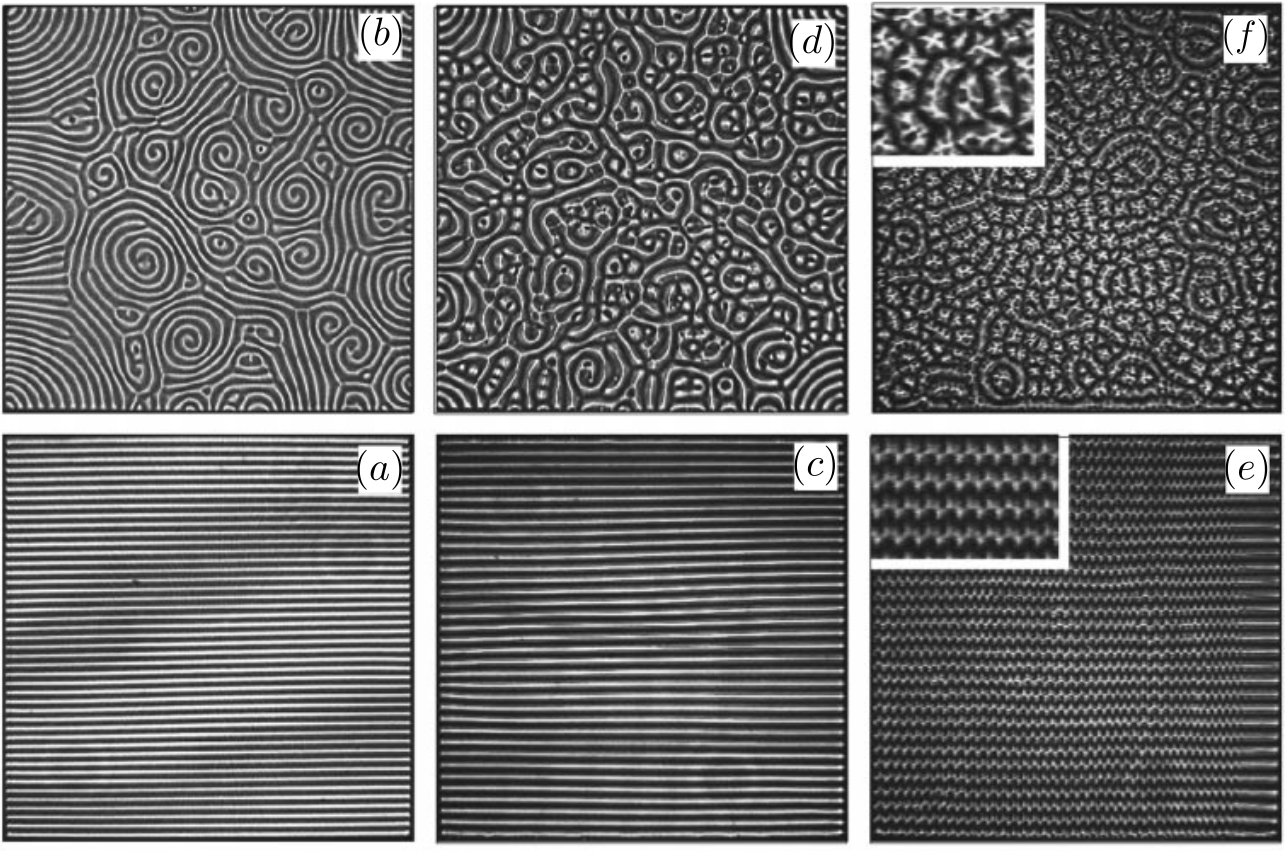
\includegraphics[width=\textwidth]{Background/Figures/bistability.png}
    \caption{The coexistence of spiral defect chaos (SDC, top row) and ideal straight rolls (ISRs, bottom row) at (a,b) $Ra = 3279$, (c,d) $Ra = 6832$ and (e,f) $Ra = 10384$. The domain size is $\Gamma = 50$ and $Pr = 1$, adapted from \cite{cakmur_bistability_1997}.}
    \label{fig:sdc_isr}
\end{figure}
However, the SDC attractor have been found to be unstable at $Pr = 4$, decaying towards ISRs over long periods \citep{bajaj_competition_1997}.
SDC has also been modalled in numerical simulations of the two-dimensional Swift-Hohenberg equations \citep{swift_hydrodynamic_1977,xi_spiral_1993,xi_spatiotemporal_1995,schmitz_spiral-defect_2002,karimi_exploring_2011}.
The critical Rayleigh number for the onset of SDC, $Ra_s$, depends on the domain's aspect ratio, and Prandtl number \citep{hu_convection_1995,bajaj_competition_1997,cakmur_transition_1997,bodenschatz_recent_2000}, and remain inconclusive.
% Investigations into quantifying the onset of SDC in terms of Rayleigh number remain inconclusive as it appears to depend on the domain's aspect ratio, and Prandtl number \citep{hu_convection_1995,bajaj_competition_1997,cakmur_transition_1997,bodenschatz_recent_2000}.
% The critical reduced Rayleigh number for the onset of SDC, $\varepsilon_s$, has been observed to decrease with increasing $\Gamma$, and increase with increasing $Pr$ \cite{hu1995a, hu1995b, bajaj1997, Cakmur97, bodenschatz2000}.
Notably, SDC has been reported in large domains ($\Gamma \gtrsim 20$), implying that there is a minimal $\Gamma$ for SDC to occur \citep{bodenschatz_recent_2000}, supporting the dependence of the $Ra_{s}$ on $\Gamma$.
The chaotic properties of SDC is also dependent of aspect ratio, where the leading Lyapunov exponents decreases with aspect ratio \citep{egolf_mechanisms_2000, paul_extensive_2007}.
Investigations into the spatial-temporal description of SDC such as the averaged roll-curvature \cite{hu_convection_1995}, probability distribution of spirals \cite{ecke_excitation_1995, liu_spiral-defect_1996} and correlation length-/time-scales \citep{morris_spiral_1993, morris_spatio-temporal_1996, cakmur_transition_1997} have been undertaken. 
Specifically, the correlation length-scales \citep{morris_spiral_1993, morris_spatio-temporal_1996, cakmur_transition_1997} scales exponentially with $Ra$, suggesting that onset of SDC from ISRs mimicks a phase transition.
Spatiotemporal chaotic behaviour similar to SDC has been found also in other pattern-formation systems such as rotational RBC \cite{hu_convection_1997}, dielectric barrier discharge \cite{dong_observation_2005} and advection diffusion reaction systems \cite{affan_spiral_2014}.

% Given the co-existence of ISRs and SDC in the parameter space of $\varepsilon$, it is known that they form bistability at $Pr \approx 1$ in a spatially extended domain, supported by experiments over a range of $\varepsilon(>0)$ \cite{Cakmur97}.
% The chaotic state of SDC is unstable at $Pr=4$, where multiple spiral patterns coarsen into a single spiral, before evolving into straight-curved rolls over a long period \cite{bajaj1997}.

% For large aspect ratios, $\Gamma \gtrsim  20$, convection rolls can exhibit spatiotemporal chaotic behaviour, known as spiral defect chaos (SDC) within the same $Ra$ range \citep{Morris93,Decker94,hu1995b,morris1996,Cakmur97,ahlers1998,egolf1998,chiam2003,vitral2020}.
% It is now established that both SDC and ISR can coexist at the same $Ra$, forming a bistable system confirmed experimentally \citep{Cakmur97}.

% HYSTERSIS
% Experimental investigations of RBC in moderate domain sizes ($\Gamma  = L/d \approx 14$ refers to the domain's aspect ratio) in rectangular (straight rolls) and cylinderical (concentric rolls) domains showed that the wavenumbers are confined within the Busse balloon.
% Depending on $Pr$, either mechanism could arise, increasing the effective roll wavenumber of the stability to adhere within the stability boundaries of the Busse balloon.
% For higher roll wavenumbers instabilities, the skewed-variose secondary instabilities arise, described by roll-pinching and merging where the effective roll-wavenumber is reduced to fall within the Busse balloon.
% At higher $Ra$, the oscillatory (OS) instability appears for $Pr \lesssim 1$ while the knotted stability appear for higher $Pr$.
% The oscillatory instability forms oscillatory ISRs reported by \cite{willis_oscillatory_1970}, while the knotted instability leads to spoke-liked covection patterns.
% , the cross roll (CR),  zig-zag and the well known Eckhaus secondary instabilties emerge.
% Lastly, the onset of a generic Eckhaus instability leads to either a roll destruction or emergence to stay within the Busse balloon.
% We will focus the secondary instabilities at $Pr = 1$ in this thesis.

% At $Pr \approx 1$, the secondary instabilities for large wavelengths are delimited by the cross-roll (CR) instability and the Eckhaus instability (not shown).
% The CR instability generates an addition roll orthogonal to the existing roll which increasing the effect roll wavenumber.
% Depending of the initial roll wavenumber, the Eckhaus instability either generates an additional or destroy rolls so that the stability boundaries are adhered to.
% The secondary instabilities for small wavelengths are delimited by the skewed-varicosed instability, where adjacent rolls pinches and merge wher a new ISR emerge adhering to the stability boundaries.

% For high Prandtl number fluids, the zig-zag instability occurs at small wavenumbers, causing wavy distortions.

 % long-wavelength modulation instabilities, where the disturbance wavenumber $|\mathbf{s}| \ll |\mathbf{q}|$ perturbs the ISR pattern. Depending on the direction and structure of the perturbation, one observes different instability types: the Eckhaus instability (ECK), involving modulations of roll spacing with $\mathbf{s} \parallel \mathbf{q}$; the zig-zag instability (ZZ), characterised by undulations along the roll axis with $\mathbf{s} \perp \mathbf{q}$; and the more general skewed varicose instability (SV), which encompasses both. For Prandtl numbers near unity ($Pr \approx 1$), SV instabilities delineate the high-wavenumber ($q$) boundary of the Busse balloon.

% In contrast, at low Prandtl numbers ($Pr \ll 1$), an oscillatory instability limits the stability region from above. This mode, marked by $\text{Im}(\omega(k)) \neq 0$ and $\mathbf{s} \approx \mathbf{q}$, leads to time-dependent behavior with propagating wave patterns and significant vertical vorticity. Additionally, short-wavelength instabilities can destabilize the ISR pattern through disturbances with $|\mathbf{s}| \approx |\mathbf{q}|$ but at a finite angle relative to $\mathbf{q}$. For $Pr \approx 1$, the cross-roll instability (CR) becomes prominent at small $q$, where new rolls form orthogonally to the original ones, preventing the development of overly short-wavelength patterns.

% Despite the idealised assumptions underlying the Busse balloon, experiments \citep[see][]{egolf_dynamical_1998} have demonstrated that its stability boundaries remain locally applicable to patches of ISR even in more disordered or weakly turbulent regimes. As such, the Busse balloon remains a central tool in understanding the transition from regular convection patterns to spatiotemporal complexity in Rayleigh–Bénard convection.
% Depending on the value of the Prandlt number, different types of secondary instabilities may arise, secondary instabilities may arise.
% % The secondary instabilities of thermal convection rolls are crucial for understanding the transition to more complex flow patterns.
% In low Prandtl number fluids, the oscillatory instability appears dominant, characterised by oscillations propagating along the ro, and the knot instability, a modification of the cross-roll instability that introduces a spoke pattern form of convectionlls.
% For intermediate $Pr$, skewed varicose instability, causing in a merging of neighbour rolls elongating the wavelength of the rolls.
% These instabilities, arising from different physical mechanisms related to momentum and heat transfer, dictate the stability and evolution of convection patterns as parameters like the Rayleigh and Prandtl numbers change.

% It is noted that weakly nonlinear stability analysis is only limited to $Ra$ slight above $Ra_c$ \citep{busse_oscillatory_1972}.
% As noted by \cite{busse_oscillatory_1972}, the applicability of weakly nonlinear analysis to slightly above onset, 
%which has been found to be a secondary instability of stationary convection rolls with complex eigenvalues.
% The theoretical foundations of performing stability analysis using expansion in powers of amplitude  (\emph{weakly nonlinear analysis}) was considered by \cite{eckhaus_studies_1965}, in which he applied it to the problem of parallel shear flows.
% The important contribution was that slightly above the onset, stable stationary rolls are found within the range of $Ra > Ra_c + 3\eta(\alpha - \alpha_c)^2$, where $\eta = \frac{1}{2}\frac{\partial Ra}{\partial \alpha}|_{Ra_c}$.
% \cite{busse_instabilities_1971} then extended the same technique to Rayleigh-B\'{e}nard convection, in which $\eta$ was found to depend on $Pr$.


% To complicate the subject further, ISRs appear to be an exception rather than the rule \citep{croquette_convective_1989-1} as multiple `non-ISR' states, in the form os squares, travelling/stationary targets, giant rotating spirals and oscillatory convection patterns have been found over the years \citep{croquette_convective_1989,croquette_convective_1989-1,plapp_dynamics_1998,hof_flow_1999,rudiger_pattern_2000,boronska_extreme_2010,boronska_extreme_2010-1}.
% For example, investigations of cylinderical RBC in small aspect-ratio revealed eight stationary statesand two oscillatory states.
% These findings were later supported by numerical experiments and bifurcation analyses.

% \begin{enumerate}
%     \item Saturated States
%     \item Busse balloon for Pr = 1
%     \item Skew-varicose, Eckhaus, Cross-roll instabilities
%     \item Low $Pr$ and high $Pr$.
%     \item What happens above the Busse balloon?
% \end{enumerate}
% 
% \begin{enumerate}
%     \item Statisitical description of spatial-temporal chaos (i.e correlation length, time etc..)
%     \item Challenge with quantifying the onset
% \end{enumerate}

% \subsection{Turbulent Rayleigh Benard: ultimate regime vs classical regime
% \begin{enumerate}
%     \item Onset of turbulence RBC
%     \item Introduce classical vs ultimate regime and scaling arguments of $Nu$.
% \end{enumerate}


%%%%%%%%%%%%%%%%%%%%%%%%%%%%%%%%%%
% Rayleigh Benard Poiseuille flows
%%%%%%%%%%%%%%%%%%%%%%%%%%%%%%%%%%

\section{Rayleigh-B\'{e}nard Poiseuille (RBP) flows}\label{sec:bkgrd_RBP}

% The RBP system consist of the primary instabilities of the RBC and RBP configurations and in the limiting cases, we observe the onset of convection rolls at $Ra_c = 1708$, and Tollmien Schlicting waves at $Re = 5772$.
\begin{figure}[h]
    \centering
    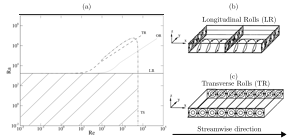
\includegraphics[width=\textwidth]{Background/Figures/RBP/RBP.pdf}
    \caption{(a) Neutral stability curves of longitudinal rolls (LR), oblique rolls (OR), transverse rolls (LR) and Tollmien-Schlicting (TS) waves, adapted from \cite{john_soundar_jerome_transient_2012}. The shaded area refers to damped perturbations. Sketch of (b) longitudinal and (c) transverse rolls, adapted from \cite{kelly_onset_1994}.}
    \label{fig:primary_instabilities}
\end{figure}

The neutral stability curves in the Rayleigh-B\'{e}nard Poiseuille (RBP) comprising of both plane Poisueuille flow (PPF) and Rayleigh-B\'{e}anrd convection (RBC) systems, are bounded by the onset of Tollmien-Schlicting waves at $Re_{c} = 5772.22$ \citep{orszag_accurate_1971}, and by the onset of convection rolls at $Ra_c = 1708$ \citep{pellew_maintained_1940}, respectively.
The imposed mean Poiseuille flow in the RBP system breaks the rotational invariance of the convection rolls, categorising them based on their orientation to the mean flow direction, namely: longitudinal ($\alpha= 0, \beta \neq 0$), transverse ($\alpha \neq 0, \beta = 0$) and oblique rolls ($\alpha \neq 0, \beta \neq 0$).
% Due to the imposed mean flow, the convection rolls are not rotationally invariant, and their orientation with respect to the mean matters.
% Generally, convection rolls that are aligned, diagonal and perpendicular to the mean flow are referred to longitudinal, oblique and transverse rolls.
The primary instabilities leading to these rolls were first investigated by \cite{gage_stability_1968} in an infinitely extended layer.
For the onset of longitudinal rolls, the linearised system reduces to that of RBC.
Hence, the critical Rayleigh number for the onset of longitudinal rolls remains the same, $Ra_{\parallel} = Ra_{c} = 1708.8$ with a critical wavenumber, $\alpha_{\parallel} = \alpha_{c} = 3.13$ \citep{pellew_maintained_1940, kelly_onset_1994}, independent of both Reynolds number, $Re$, and Prandtl number $Pr$.
In contrast, the onset of transverse rolls exhibits a critical Rayleigh number, $Ra_\perp = f(Re,Pr)$, that increases with $Re$ and is dependent on $Pr$ \citep{gage_stability_1968, muller_transversal_1992, nicolas_two-dimensional_1997}.
The critical Rayleigh number for the onset of obliqued rolls can be obtained by applying a Squire transformation \citep{squire_stability_1933} to the linearised problem for transverse rolls.
For a given $Ra$, the corresponding critical $Re$ for the onset of oblique rolls is higher than that of transverse rolls \citep{gage_stability_1968}.
% The critical Rayleigh number for the onset of obliqued rolls are obtained by performing a Squire transformation on the linearised transverse roll system where for a given $Ra$, the critical $Re$ of oblique rolls is higher than the critical $Re$ for transverse rolls \citep{gage_stability_1968}.
The neutral stability curves associated with the transverse rolls (TR), oblique rolls (OR) and longitudinal rolls (LR) are shown in figure \ref{fig:primary_instabilities}.

Experimental observations of the onset of longitudinal rolls have been reported in channels with large transverse aspect ratios (i.e span-to-depth) \citep{akiyama_experiments_1971,ostrach_heat_1975,fukui_longitudinal_1983}, while the onset of transverse rolls are observed in narrower channels \citep{luijkx_existence_1981,ouazzani_etude_1989,ouazzani_etude_1990}.
Indeed, linear stability analysis conducted for finite channels revealed that critical Rayleigh number $Ra_\parallel$ remains independent for transverse aspect ratios greater than five, and increases quickly below that.
Therefore, the critical Rayleigh number for onset of transverse rolls, $Ra_\perp$, is lower than $Ra_\parallel$ in narrow channels for small Reynolds numbers \citep{nicolas_linear_2000}, providing support for the preference of transverse rolls in narrow channels.
% Indeed, linear stability analysis of narrow channel reveal that the $Ra_{\parallel}$ are increased relative to the $Ra_\perp$ for small $Re$ \citep{nicolas_linear_2000}.
\cite{ouazzani_etude_1990} reported laminar Poiseuille flow in the $Ra, Re$ parameter space where transverse rolls are expected based on temporal linear stability analysis.
% However, linear temporal stability analysis failed to explain the experimental results from \cite{ouazzani_etude_1990}, where a laminar Poiseuille is observed in the parameter space where transverse rolls are expected.
This contraction was address by \cite{muller_transversal_1992}, who showed that transverse rolls can be either convectively or absolutely unstable, and the boundary between them matches with the experimental results of \cite{ouazzani_etude_1990}.
By considering the response from three-dimensional impulse, \cite{carriere_convective_1999} further demostrated that the longitudinal rolls, unlike the transverse rolls, are always convectively unstable.
% The critical Rayleigh number for oblique and transverse rolls matches that of RBC at $Re=0$ due to horizontal isotropy, but increases as $Re$ increases, depending on $Pr$, i.e., $Ra_{\perp} = f(Re,Pr)
Nonmodal stability analysis of subcritical RBP, $Ra < Ra_c, Re < Re_{c}$, performed by \cite{john_soundar_jerome_transient_2012} revealed that the optimal transient growth is primarily dominanted by streamwise rollers of plane Poiseuille flow \citep{reddy_energy_1993}, with a spanwise wavenumber of $\beta_{opt} \approx 2.05$.
The maximum amplifcation factor, $G_{max}$ increases modestly with $Ra$, and the critical wavenumber approaches, $\alpha_{\parallel}$, indicative of longitudinal rolls.
% Nonmodal stability analyses of subcritical RBP indicate that the optimal transient growth $G_{max}$ increases gradually with $Ra$.
% The wavenumber of the optimal initial conditions, $\beta_{max}$, resembles that observed in shear flows \citep{reddy_energy_1993}, and gradually approaches the critical wavenumber of convection rolls, $\alpha_{\parallel}$, as $Ra$ increases \citep{john_soundar_jerome_transient_2012}.
% For $Re > 0$, the longitudinal rolls appear as the dominant primary instability \citep{gage_stability_1968}.
Since longitudinal rolls are the dominant primary instability for $Re > 0$ in infinite domains, their secondary stability have been analysed by \cite{clever_instabilities_1991}.
Their study revealed the presence of a secondary, time-dependent wavy instability near $Re \sim 100$ \citep{clever_instabilities_1991}, leading to the onset of tertiary solutions in the form of wavy rolls.
These have been observed experimentally and was found to be convectively unstable \citep{pabiou_observations_2003, pabiou_wavy_2005, nicolas_characterisation_2010}.
\cite{clever_instabilities_1991} also speculated that the wavy rolls are less efficient at transporting heating than longitudinal rolls at the same control parameters, confirmed numerically \citep{nicolas_influence_2012}.
The impact of finite transverse aspect ratios on the onset of wavy rolls have been also studied \citep{xin_stability_2006, nicolas_characterisation_2010}, where the critical $Ra$ was found to be approximatgely 1.5 times higher than that in an infinite domain \cite{clever_instabilities_1991}.
The influence of external excitations on the development length of wavy rolls have been explored.
An increase in external excitation amplitude have shown to reduced the required development length of wavy rolls \citep{nicolas_characterisation_2010,nicolas_influence_2012}.
More recently, studies of turbulent RBP flows showed that shear-driven turbulence can enhance heat fluxes \citep{scagliarini_heat_2014, scagliarini_law_2015, pirozzoli_mixed_2017}.
% In finite streamwise extensions of RBP flows, the onset of convection rolls and the heat flux variations due to entrance effects have been investigated \citep{mahaney_effect_1988,lee_effect_1991,nonino_laminar_1991}.
Extensions of the RBP configuration, such as flows over wavy walls or with sinusoidal thermal forcing have been investigated, potentially offering a reduction in drag and enhancing heat transport \citep{hossain_drag_2012,hossain_drag_2016,hossain_role_2020}.
% RBP flows with sinusoidal heating and wavy walls have also been studied \citep{hossain_spectral_2021}.
For a comprehensive overview of RBP flows, the reader is referred to the reviews by \cite{kelly_onset_1994} and \cite{nicolas_revue_2002}.

%%%%%%%%%%%%%%%%
% THESIS OUTLINE
%%%%%%%%%%%%%%%%

\subsection{Thesis Outline}\label{sec:thesis_outline}

% The governing equations of the fluid motion in given by the Navier-Stokes equations with Boussinessq approximations,
% \begin{equation}
%     \frac{\partial \mathbf{u}}{\partial t} + (\mathbf{u} \cdot \nabla) \mathbf{u} = -\frac{1}{\rho} \nabla p + \nu \nabla^2 \mathbf{u} + g\beta(T-T_0).
% \end{equation}`
% \begin{equation}
%     \frac{\partial T}{\partial t} + (\mathbf{u} \cdot \nabla)T = \kappa \nabla^2 T,
% \end{equation}
% \begin{equation}
%     \nabla  \cdot \mathbf{u} = 0.
% \end{equation}
% with arbitrary Dirichlet and Neumann boundary conditions.
% \begin{equation}
%     \mathbf{u}_d, p_d, T_d \in \Omega_d, \quad \nabla\mathbf{u}_N, p_N, T_N \in \partial\Omega_N.
% \end{equation}
% where $\mathbf{u}, T, p$ refers to the velocity, temperature and pressure fields, primitive variables that are not known a priori and $\rho, \nu, \kappa$ refers to the properties of the fluid, namely, density, kinematic viscosity and thermal diffusivity.
% For a given set of fluid properties $\rho, \nu, \kappa$ and geometric properties $L^*, t^*, u^*$ referring to an arbitrary length-, time- and velocity-scale, we are primarily interested in the behaviour of the fluid i.e if its laminar or turbulent.
% In other words, we have a six control parameters that describes a fluid flow of interest.
% To reduce the number of control parameters, we can suitably nondimensionalise the primitive variables by a velocity scale $u_c$, length scale, $L_x$, and time scale $u_c/L_x$, where $u_c$ refers to the centreline velocity of a laminar flow and $L_x$ refers to the streamwise length of the domain.
% The nondimensional equations with Boussienessq approximations are now given as,
% \begin{equation}
%     \frac{\partial \mathbf{u}}{\partial t} + (\mathbf{u}\cdot\nabla)\mathbf{u} = -\nabla p + \frac{1}{Re}\nabla^2 \mathbf{u} + \frac{Ra}{Re^2Pr} \theta
% \end{equation}
% \begin{equation}
%     \frac{\partial \theta}{\partial t} + (\mathbf{u} \cdot \nabla)\theta = \frac{1}{RePr}\nabla^2 \theta,
% \end{equation}
% \begin{equation}
%     \nabla \cdot \mathbf{u} = 0.
% \end{equation}
% where $\mathbf{u}, \theta, p$ refers to the nondimensionalised velocity, temperature and presure.
In this thesis, I am particularly focused on the transition behaviour of fluid flow driven by shear and bouyancy, addressing questions related to the onset of instabilities due to shear and buoyancy, and the (possible) competitive between shear and buoyancy driven instabilities.
I would like to preface that while this thesis is dealing with onset of instabilities, it does not clearly indicate that the onset of such instabilities necessarily lead to turbulence, hence, for terminology sake, we shall be looking into transitional regimes where the fluid neither laminar nor turbulent.
The main motivations are two-folds, both from an academic and applied point-of-view. 
Within academia, the onset and transition to turbulence in Rayleigh-B\'{e}nard Poiseuille flows remains poorly understand.
Whilst there had been significant progress in our understand of transition to turbulence in independent setups, Rayleigh-B\'{e}nard convection and plane Poiseuille flows, their combined effects are not known.
The thesis is structured into the follow, Chapter 1 is the introduction with literature review, chapter 2 methodology assosicated with the spectral/\emph{hp}-element method, chapter 3 with results related to the the Rayleigh and Reynolds number sweep, chapter 4 with a specific focus on the bistability between spiral defect chaos and ideal straight rolls and finally chapter 5 with concluding remarks.

\begin{enumerate}
   \item Academic motivation - flow structures, statistics, transition.
   \item Application motivation - shear, heat transfer. Chip cooling, thin-film fabrication and atmospheric boundary layer.
\end{enumerate}
We seek to investigate the influence of unstable stratification quantified by Rayleigh number $Ra$, on the behaviour tuburlent-laminar bands. 
The onset of convection occurs at a critical Rayleigh number of $Ra_c > 1708$, in the form of a pair of convection rolls.
When aligned in the streamwise direction, the convection rolls are seemingly analogous to a pair of counter-rotating vortices, an optimal initial condition for transient growth. 
Our investigation naturally answers a few questions related to turbulent-laminar bands.
For example, does the onset of turbulent-laminar bands, $Re_{cr}$ decrease with increasing $Ra$?
Do $Ra$-effects influence the structure of turbulent-laminar bands i.e band angle/width? 

The answers to our research will have important implications Rayleigh-B\'{e}nard Poiseuille flows, ubiquitous in atmospheric, geophysical and engineering flows.

    % \chapter{Numerical Techniques}\label{chap:3}
We will discuss the fundamentals of numerical methods relevant to solving the Navier-Stokes equations.
We begin the discussion of the weighted of residuals (\S \ref{sec:methodofweightedresiduals}) and the spatial discretisation using spectral/\emph{hp} element methods in one dimension (\S \ref{sec:spectralhpelementmethods}).
This is followed by techniques for solving the Navier-Stokes equations (\S \ref{sec:numeraltechniquesforNS}), introducing the velocity-correction scheme, enforcing a constant flow rate and the quasi-3D approach for semi-homogeneous domains. 
This chapter concludes with numerical techniques for the stability analysis of the Navier-Stokes equations (\S \ref{sec:stabilityanalysisofNS}), including eigenvalue computation and edge tracking.
% In this chapter, I will present the numerical methods ultilised in this thesis.
% The premise of numerical methods is to solve for the the partial differential equations, the Navier-Stokes equations.
% The incompressible Navier-Stokes equations describe the time- and spatial-varying velocity field and pressure field.
% One of the foundations of solving partial differential equations begin with the method of weighted residuals. 

%%%%%%%%%%%%%%%%%%%%%%%%%%%%%%%%%%
% 3.1 METHOD OF WEIGHTED RESIDUALS
%%%%%%%%%%%%%%%%%%%%%%%%%%%%%%%%%%

\section{Method of weighted residuals}\label{sec:methodofweightedresiduals}
Spatial discretisation errors, or residuals, arises as one seeks an approximate solution to some partial differential equation (PDE).
The method of weighted residual provides a generic mathematical framework in which constraints on the residual could be applied flexibly, defining the spatial discretisation scheme and its convergence properties.
In summary, we approximate the solution of PDE by considering a finite expansion of a suitable basis, to which its coefficients are sought after by minimising the inner product between the PDE and a test (or weight) function.
To demonstrate this, we consider a linear partial differential equation as,
\begin{equation}\label{eq:linear_operator}
    \mathbf{L}[u(x)] = 0, \quad x \in \Omega,
\end{equation}
where $\mathbf{L}$ refers to a linear spatial differential operator subjected to some boundary conditions within the domain, $\Omega$, while $u(x)$ refers to the exact solution of $\mathbf{L}$.
Examples of PDEs with linear spatial differential operators include the Laplace equation, $\nabla^2 u = 0 $, Poisson equation, $\nabla^2 u = f$, and the Helmholtz equation, $\nabla^2 u + \lambda u  = f$.
We suppose that the exact solution $u(x)$ can be approximated (discretised) by $N$ finite number of basis (or expansion) functions, $\Phi(x)$.
\begin{equation}\label{eq:approximate}
    u(x) \approx u^\delta(x) = \sum_{i=0}^{N-1} \hat{u}_i \Phi_i(x),
\end{equation}
where $u^\delta(x)$ refers to the approximate solution of $u(x)$, consisting of a linear combination of the product between the $i^{th}$ basis coefficient, $\hat{u}_i$, and the $i^{th}$ global basis expansion, $\Phi_i(x)$, defined within $\Omega$.
Since $u^\delta(x)$ is an approximate solution of equation \eqref{eq:helmholtz}, we expect a residual (or `error') between the exact solution, $u(x)$, and $u^\delta(x)$,
\begin{equation}\label{eq:residual}
    \mathbf{L}[u^\delta(x)] = R[u^\delta(x)],
\end{equation}
where $R[u^\delta(x)]$ refers to the residual which depends on the approximate solution $u^\delta(x)$ and varying within $\Omega$.
In other words, equation \eqref{eq:helmholtz} might not be satisfied everywhere in $\Omega$. 
We need to place restrictions on the residual, such that it the residual approaches zero, $R \rightarrow 0$, and the approximate solution approaches the exact solution, $u^\delta(x) \rightarrow u(x)$.
The method of residuals places a restriction on the residual by applying an inner product between the governing equation, and $N$ test (or weight) functions, $v_j(x)$, and setting it to zero,
\begin{equation}\label{eq:weightinnerresidual}
    (v_j(x), R[u^\delta(x)]) = 0, \quad j = 0, ..., N-1.
\end{equation}
\begin{definition}[Inner product]
The inner product between two functions $f(x)$ and $g(x)$ is,
\begin{equation}
       (f, g) = \int_\Omega f(x) g(x) dx \nonumber.
\end{equation}
\end{definition}
% where $(\, \cdot \, , \, \cdot \,)$ refers to an inner product, a measure of orthogonality between function $f(x)$ and $g(x)$ defined as,
% \begin{equation}\label{eq:inner-product}
%        (f, g) = \int_\Omega f(x) g(x) dx.
% \end{equation}
By setting equation \eqref{eq:weightinnerresidual} to zero, it becomes a system of $N$ ordinary differential equations, where the $N$ basis coefficients, $\hat{u}_i$.
The choice of test function defines the projection methods, and examples of projection methods are shown in table \ref{tab:weightFunction}.
We emphasise that the method of weighted residuals merely describes the projection method, but does not specify the type of basis expansions, as we will discuss later in \S \ref{sec:spectralhpelementmethods}.
The choice of projection method coupled with suitable basis expansions will have different solution convergence properties.
A particular interest is on how quickly the residual vanishes as the number of basis expansions increases.
For instance, by considering the Galerkin method coupled with Fourier expansions, one can expect exponential convergence, desirable for an efficient representation of turbulent dynamics.
% Certain mathematical properties such as spectral convergence as desired in the case of Galerkin projection using Fourier expansions, 
% The choice of \emph{trial} functions used in \emph{nektar++} will be elaborated in Section \ref{sec:modifiedBasis}.
% the method of weighted residuals is only restrictive to the weight
% Table \ref{tab:weightFunction} shows the different forms of weight functions and its corresponding numerical method.
\renewcommand{\arraystretch}{1.5} % Default value: 1
\begin{table}[h]
    \centering
        \begin{tabular}{cc}
            Weight functions & Projection method \\
            \hline
            $v_j(x) = \delta(x-x_j)$ & Collocation \\
            $v_j(x) =\left\{\begin{array}{ll}
                1 & \mbox{if } x \in \Omega_j\\
                0 & \mbox{if } x \notin \Omega_j \\
           \end{array}\right. $& Finite-Volume \\
            $v_j(x) = \phi_j$& Galerkin \\
            $v_j(x) = \frac{\partial R}{\partial \hat{u}_j}$ & Least-squares \\
            \hline
        \end{tabular}
        \caption{Examples of weight functions and projection methods}
    \label{tab:weightFunction}
\end{table}
% For instance, for $v_j = \delta(x-x_j)$, the numerical method becomes the \emph{collocation} method where the differential equation is satisfied on discrete points $x_j$.
% The type of restriction on the residual is implemented through the choice of \emph{test} function, $v_j$.
\section{Galerkin Projection}\label{sec:galerkinprojection}
The Galerkin projection remains a standard projection method in the context of the finite element method, where the test functions, $v(x)$, are chosen to be lie in the same functional space as the global basis functions, $\Phi(x)$.
To demostrate the Galerkin projection method, we consider that the differential operator earlier in equation \eqref{eq:linear_operator} as a 1D Helmholtz equation,
\begin{subequations}\label{eq:helmholtz}
    \begin{equation}
        \mathbf{L}[u(x)] \equiv \frac{\partial^2 u(x)}{\partial x^2} - \lambda u(x) - f(x) = 0, \quad x \in \Omega := [0, l]
    \end{equation}
    \begin{equation}
        u(0) = g_D, \quad \frac{\partial u}{\partial x}\Big|_{x=l} = g_{N}.
    \end{equation}
\end{subequations}
where $\lambda$ is a real positive constant, $f(x)$ is a forcing function, and $\Omega$ refers to the spatial domain bounded between $0$ and $l$. 
% $ hh u(x), \lambda, f, \Omega$ refers to the linear (spatial) differential operator, solution to the diffential equation, a real positive constant, forcing function and the spatial domain bounded between 0 and $l$, respectively.
To ensure that problem is well posed, Dirichlet and Neumann boundary conditions, $g_D$ and $g_N$, are imposed at $x = 0$ and $x = l$ respectively.
% In order for the problem to be well-posed, we impose both Dirichlet and Neumann, boundary conditions corresponding to $g_D$ and $g_N$ at $x= 0 $ and $x=l$, respectively.
Equation \ref{eq:helmholtz} is commonly referred to as the strong or classical form.

The subsequent step in Galerkin projection methods is take the inner product of the equation \eqref{eq:helmholtz} with a test function, $v(x)$, that satisfies the homogeneous Dirichlet boundary conditions by definition, i.e. $v(0) = 0$, and setting the inner product to zero,
\begin{equation}\label{eq:helmholtz_inner}
    (v(x), \, \mathbf{L}[u(x)]) = \int_0^l w\left[\frac{\partial^2 u(x)}{\partial x^2} - \lambda u(x) + f(x)\right] \mathrm{d}x =  0.
\end{equation}
This step is equivalent to applying the method of weighted residuals (\S \ref{sec:methodofweightedresiduals}), where $u(x)$ could refer to the approximate solution, $u^\delta(x)$. 
Next, we perform integration by parts,
\begin{equation}\label{eq:weak_form}
    \underbrace{\int_0^l \frac{\partial v}{\partial x}\frac{\partial u}{\partial x} \, \mathrm{d}x + \int_0^l \lambda v u \, \mathrm{d}x}_{a(v,u)}= \underbrace{\int_0^l v f \, \mathrm{d}x + \left[ v \frac{\partial u}{\partial x} \right]_0^l}_{f(v)}.
\end{equation}
This equation is typically referred to as the weak \footnote{The notions of the \emph{weak} and \emph{strong} are refers to the smoothness (regularity) required of admissible solutions. In the weak formulation, the highest derivative involved is up to first-order, so the solution space is $H^1$. This space is generally larger than that of the strong formulation, which required $u \in \mathcal{H}^2(\Omega)$. Since $H^2(\Omega) \subset H^1(\Omega)$ the weak formualation imposesd a `less stringent' constraint of the solution space of admissible functions.} form of equation \eqref{eq:helmholtz}.
In compact notation, we define the bilinear and linear forms as,
\begin{subequations}
    \begin{equation}
        a(v,u) = f(v),
    \end{equation}
\end{subequations}
where $a(v,u)$ and $f(v)$ are typically refered to as the strain energy and forcing function in structural mechanics, required to remain finite.
To ensure this, we restrict the choice of solutions $u(x)$ to lie in the solution space, $\mathcal{U}$, defined as
\begin{equation}\label{eq:solution_space}
    \mathcal{U} := \{ u \, | \, u \in H^1(\Omega), u(0) = g_D \},
\end{equation}
% where $u \in H^1$ contains functions of $u$ in the Sobolev space such that the Dirichlet condition $u(0) = g_D$ is statisfied and the sum of square integral of $u$ and its first derivatives, $\frac{\partial u}{\partial x}$ remains bounded,
where $u \in H^1$ refers to functions of $u$ belonging to Sobolev space of order 1, and satistfying the Dirichlet condition, $u(0) = g_D$,  at $x = 0$.
\begin{definition}[Sobolev space]
    We define Sobolev space of order $n \geq 1$ on $\Omega$,
    \begin{equation}
        H^n(\Omega) = \{u \, | \, u \in L_2(\Omega), D^\alpha u \in L_2(\Omega), \forall \alpha : \alpha \leq n\}, \nonumber
    \end{equation}
    where $D^\alpha u$ refers to derivatives up to order $\alpha$ and $L_2(\Omega)$ refers to functions that are square integrable.
\end{definition}
\begin{definition}[$L_2$ space]
    The space $L_2(\Omega)$ refers to functions that are square integrable,
    \begin{equation}
        (u, u)_{L_2} = \int_\Omega |u(x)|^2 \, \mathrm{d}\Omega < \infty. 
    \end{equation}
\end{definition}
We consider admissible functions up to the first derivatives, the highest order derivative in the weak formulation of equation \eqref{eq:helmholtz_inner}.
Similarly, the space of test functions, $\mathcal{V}$, is defined as,
\begin{equation}\label{eq:test_space}
    \mathcal{V} := \{ v \, | \, v \in H^1, v(0) = 0 \},
\end{equation}
where $v \in H^1$ are refer to test functions belonging to the Sobolev the space of order 1, and is defined to be zero, $v(0) = 0$ on Dirichlet boundary condition, $x = 0$.
The generalised weak form is therefore finding $u(x) \in \mathcal{U}$, such that
\begin{equation}\label{eq:bilinear_infinite}
    a(v,u) = f(v), \quad \forall v \in \mathcal{V}.
\end{equation}
At this point, equation \eqref{eq:bilinear_infinite} is infinite dimension as the function spaces, $\mathcal{U}$ and $\mathcal{V}$, contain infinitely many functions.
% This formulation is infinite dimensional, as the function space $\mathcal{U}, \mathcal{W}$ contain infinitely many functions.
To obtain an approximate solution, $u^\delta(x)$, we restrict ourselves to finite dimensional subspaces, $\mathcal{U}^\delta \subset \mathcal{U}$, and $\mathcal{V}^\delta \subset \mathcal{V}$.
The problem is then to find $u^\delta \in \mathcal{U}^\delta$, such that
\begin{equation}
    a(v^\delta, u^\delta) = f(v^\delta), \quad v^\delta \in \mathcal{V}^\delta.
\end{equation}
Here, the subspaces $u^\delta \in \mathcal{U}^\delta$ and $v^\delta \in \mathcal{V}^\delta$ are not the same, compare equations \eqref{eq:solution_space} and \eqref{eq:test_space}, necessary for the standard Galerkin projection procedure where they should lie in the same subspace.
To ensure that they belong to the same space, we lift the solution $u^\delta$ into two parts,
\begin{equation}
    u^\delta = u^\mathcal{H} + u^\mathcal{D}.
\end{equation}
where $u^\mathcal{H} \in \mathcal{V}^\delta$ satisfies the homogeneous Dirichlet condition (e.g. is zero on Dirichlet boundaries), belonging to the same subsapce as $v^\delta \in \mathcal{V}^\delta$, while $u^\mathcal{D} \in \mathcal{U}^\delta$ satisfies the Dirichlet boundary conditions $u^\mathcal{D}(0) = g_D$.
Hence, the standard Galerkin projection method is to search for the homogeneous solution, $u^\mathcal{H} \in \mathcal{V}^\delta$, such that,
\begin{equation}\label{eq:standard_galerkin}
    a(v^\delta, u^\mathcal{H}) = f(v^\delta) - a(v^\delta, u^\mathcal{D}).
\end{equation}
This concludes the classical Galerkin formulation. 
Under certain assumptions of $a$, a solution is guaranteed under the Lax-Milgram theorem \citep{bers_ix_1955}.
%%%%%%%%%%%%%%%%%%%%%%
% SPECTRAL/HP ELEMENTS
%%%%%%%%%%%%%%%%%%%%%%

\section{Spectral/\emph{hp} element method}\label{sec:spectralhpelementmethods}
We have described the procedure for approximating a solution of a PDE using the classical Galerkin projection technique.
However, the spatial discretisation scheme, related to the choice of basis (and test) functions, remains undiscussed.
% and describe the essential numerical differential and integral techniques.
% , equation \eqref{eq:standard_galerkin} reduces to a system of linear equations.
% To represent the spatially-dependent velocity and pressure fields, spatial discretisation is performed using the spectral/\emph{hp} element method.
% Other popular methods of spatial discretisation found in literature are the finite-difference methods, and finite-volume methods.
% The spectral/{hp} element method (SEM) is related to the Galerkin method in which the type of \emph{trial} function used. The spectral/\emph{hp} element method combines 2 traditional numerical methods, namely, 
In this section, we discuss the spectral/\emph{hp} element method \citep{patera_spectral_1984},
where the solution is partitioned into a set of non-overlapping finite elements of size $h$, consisting of a linear combinbation of continuous orthogonal polynomial functions up to order $P$.
% The spectral/\emph{hp} element method pioneered by \citep{patera_spectral_1984} is a spatial discretisation technique in which the solution domain is partitioned into a set of non-overlapping (finite) elements with size $h$, each consisting of a linear combination of continuous polynomial functions of up to order $P$. 
% represented by a polynomial of up to order $p$.
% which leverages the advantages of offering geometric flexibility by decomposing the global domain into a set of non-overlapping (finite) elements of size $h$, each consisting of a linear combination of continuous polynomial functions of up to order $p$.
It leverages the geometric flexibility of classical finite-element methods, allowing for the representation of complex engineering geometries, and the exponential (spectral) convergence properties of classical spectral methods, where the solution error decreases exponentially.
% The Spectral/\emph{hp} element method leverages the advantages of both methods - geometric flexibility and spectral covergence.
% The spectral/\emph{hp} method uses a series of high-order polynomials (Lagrange/Legendre) within each element.
Suppose we consider $P+1$ linearly independent polynomials spanning the polynomial space of $\mathcal{P}_P$, the error of a smooth solution with element size of $h$ and polynomial order $P$ has the property of \citep{karniadakis_spectralhp_2005}, 
\begin{equation}\label{eq:error_convergence}
    ||u(x) - u^{\delta}(x)|| \leq Ch^P||u(x)|| \approx O(h^P).
\end{equation}
where $C$ is some constant.
Equation \ref{eq:error_convergence} implies that the error decreases linearly with $h$, and exponentially with $P$.
This section is organised into domain partition, standard elements, assembly process, modal and nodal expansion functions, numerical integration and differentiation, concluding with an example in 1D.
% % It offers the flexibility of offering refinements in either $h$ or $p$, or both.
% \begin{enumerate}
%     \item Finite elements:
%         \subitem The finite element method decomposes the global domain into a set of non-overlapping subdomains (finite elements), represented by linear shape functions. In a 1D domain, the size of each element is given by $h$ and the approximate solution should covergence as $h$ is decreased - also known as \emph{h}-refinement. The flexibility of domain decomposition allows for complex engineering geometries to be represented. 
%     \item Spectral method:
%         \subitem The spectral method performs a global discretisation of the domain. The domain is represented by a linear combination of global continuous functions, such as the Fourier series. Spectral methods benefit from the property of \emph{spectral convergence}, where the solution error decreases by $\mathcal{O}(c^{-N})$, where $c$ is some constant $0 \leq c \leq 1$ and $N$ is the number of polynomials (\cite{trefethen_2000}). In other words, as the number of functions is increased, the error decreases exponentially.
% \end{enumerate}

%%%%%%%%%%%%%%%%%%
% DOMAIN PARTITION
%%%%%%%%%%%%%%%%%%
\subsection{Domain partition}
The first step concerns the partitioning the domain into a set of (finite) elemental regions.
We consider an example in one dimension within $\Omega$, and partition it into a set of $N_{el}$ elements, where $\Omega^e$, refers to the elemental partitions with $1 \geq e \geq N_{el}$, such that they meet at their boundaries and do not overlap,
\begin{equation}
    \Omega = \bigcup_{e = 1}^{N_{el}} \Omega^e, \quad \text{where} \; \bigcap_{e=1}^{N_{el}} \Omega^e = \emptyset
\end{equation}
where the $e^{th}$ element is defined as,
\begin{equation}
    \Omega^e = \{x \, | \, x_{e-1} \geq x \geq x_e \}.
\end{equation}
Each element can be represented by a linear combination of orthogonal basis expansions.
The basis expansions can be either modal or nodal expansions, as we shall see later.
% Each element it then represented by a linear combination, $\phi(x)$, where $x$ is referred to the \emph{global} domain.

%%%%%%%%%%%%%%%%%%%
% STANDARD ELEMENTS
%%%%%%%%%%%%%%%%%%%
\subsection{Standard Elements}
\begin{figure}[h]
    \centering
    \includegraphics[width=\textwidth]{NumericalMethods/Figures/standard_element_3elements.pdf}
    \caption{A spectral/\emph{hp} element representation of $u(x)$, consisting of three non-overlapping finite elements, each containing a linear combination of local expansion bases of up to $P=2$.}
    \label{fig:standard_element}
\end{figure}
In general, we expect to work with non-uniform elements that may have arbitrarily shapes, making the definition of basis expansions potentially unwieldy.
To simplify the formulation, it is convenient to define a \textit{standard} element,
\begin{equation}
    \Omega_{st} = \{ \xi \, | \, -1 \geq \xi \geq 1 \},
\end{equation}
where $\Omega_{st}$ refers to the standard element defined in local coordinates, $\xi \in [-1, 1]$.
Within this standard element, the formulation of basis expansions, as well as differential and integration operations, can be carried out in the local coordinate system $\xi$, before mapping the solution back to the global domain, $x$.
We can map the standard element into any arbitrary global coordinates based on a linear mapping $\chi^e:\Omega_{st} \rightarrow \Omega$,
\begin{equation}
    x = \chi^e(\xi) = \frac{1-\xi}{2} x_e + \frac{1 + \xi}{2}x_{e+1}, \quad \xi \in \Omega_{st}
\end{equation}
which has an analytical inverse, $(\chi^e)^{-1}(x)$,
\begin{equation}
    \xi = (\chi^e)^{-1}(x) = 2 \frac{x - x_{e-1}}{x_e - x_{e-1}} - 1, \quad x \in \Omega^{e}.
\end{equation}
For illustration purposes, we consider that the standard element can be represented by three local basis expansions of polynomial order of up to $P = 2$,
\begin{equation}\label{eq:def_local_expansions}
    \phi_0^e(\xi) = \frac{1 - \xi}{2}, \quad \phi_1^e(\xi) = (1 + \xi)(1 - \xi), \quad \phi_2^e(\xi) =  \frac{1 + \xi}{2},
\end{equation}
where $\phi_0^e, \phi_2^e$ and $\phi_1^e$ refers to the linear and quadratic local basis expansions of the $e^{th}$ element.
These local basis expansions is illustrated in figure \ref{fig:standard_element}.
We note that the formulations of local basis expansion here is merely an example.
In practice, the local basis expansions are usually chosen to have orthogonality properties under a certain inner product.
The approximate solution is now represented as,
\begin{equation}\label{eq:local_expansions}
    u^\delta(x) = \sum_{e=0}^{N_{el}-1}\sum_{i=0}^P \hat{u}_i^{e}\phi^e_i(\chi^e(\xi)).
\end{equation}
where $\hat{u}_i^e$ refers to the local expansion basis coefficients.
The approximate solution, $u^\delta(x)$, now lie within the solution space $\mathcal{U}^\delta$ defined as,
\begin{equation}
    \mathcal{U}^\delta := \left\{ u^\delta \,\middle|\, u^\delta \in H^1,\ u^\delta(\chi^e(\xi)) \in \phi_i^e(\xi), \forall i : 0 \leq i \leq P, \forall e : 0 \leq e \leq N_{el} \right\}
\end{equation}
% Figure \ref{fig:standard_element} presents the sketch of representing a continous function using spectral/\textit{hp} element methods for $P = 2$ and $N_{el} = 3$.

%%%%%%%%%%%%%%%%%%%%
% ASSEMBLY FUNCTIONS
%%%%%%%%%%%%%%%%%%%%

\subsection{Global assembly}
In this section, we introduce the concept of global assembly (or direct stiffness summation) which relates the global basis expansions (equation \eqref{eq:approximate}), $\Phi_i(x)$, to the local basis expansions (equation \eqref{eq:local_expansions}), $\phi_i^e(x)$, where the solution can be approximated using either formulation,
\begin{equation}
    u^\delta(x) = \sum_{i=0}^{N-1}\hat{u}_i\Phi_i(x) = \sum_{e=0}^{N_{el}-1}\sum_{i=0}^P \hat{u}_i^{e}\phi^e_i(\chi^e(\xi)).
\end{equation}
In general, we can represent the global and local basis coefficients each as a column vector,
\begin{equation}
    \mathbf{\hat{u}}_g = 
\begin{pmatrix}
    \hat{u}_0 \\
    \vdots \\ 
    \hat{u}_N
\end{pmatrix},
\quad 
\mathbf{\hat{u}}_l = 
 \begin{pmatrix}
     \mathbf{\hat{u}}^0 \\ 
     \vdots \\
     \mathbf{\hat{u}}^{N_{el}-1}
 \end{pmatrix},
\end{equation}
where $\mathbf{\hat{u}}^{e} = (\hat{u}_0^e, ..., \hat{u}_P^e)^T$, $\mathbf{\hat{u}}_g \in \mathbb{R}^N$, $\mathbf{\hat{u}}_l \in \mathbb{R}^{N_{loc}}$ and $N_{loc} = N_{el}(P+1)$.
As there can be more global degrees of freedom than local degrees of freedom, $N > N_{loc}$, we need to impose some conditions on the local expansion coefficients.
One of the common approach is to enforce $C^0$ continuity across elemental boundaries, referred to as the continous Galerkin projection.
Following the definition of local basis expansions in equation \eqref{eq:def_local_expansions}, this condition can be supplemented using,
\begin{equation}
    \hat{u}^{e-1}_P = \hat{u}^e_0.
\end{equation}
\begin{figure}[h]
\centering
\includegraphics[width=\textwidth]{NumericalMethods/Figures/standard_element_3elements_C0.pdf}
\caption{A graphical representation of $C^0$ across elemental boundaries and the relationship between local basis coefficients, $u_0^e, u_P^e$, and global basis expansions, $u_i$.}
\label{fig:local_to_global}
\end{figure}
The graphical representation of this condition enforcing $C^0$ continuity between the element boundaries for three finite elements with $P=2$ local basis expansions, and the relationship between global and local basis coefficients are shown in figure \ref{fig:local_to_global}.
% In the approach of continuous Galerkin projection methods, we enforce our solution to be $C^0$ continuous across the elemental boundaries.
% In other words, the neighbouring linear interior elements must meet at the boundaries, such that the local expansion coefficients are constrained by,
% We can ultilise a mapping b
We can relate the global and local basis coefficients with an assembly matrix, $\mathbf{A} \in \mathbb{R}^{N_{loc} \times N}$,
% This constraint by consider a mapping between the (global) expansion coefficients, and local expansion coefficients, 
% Due to the constraint described above, we need a mathematical process which maps the local coefficients to the global coefficients.
% To fulfil this description, we introduce a vector of global coefficients, $\mathbf{\hat{u}}_g$, and local coefficients $\mathbf{\hat{u}}_l$, and a linear map $\mathbf{A}$, given as,
% In this case, we introduce the definition of global modes given as,
% \begin{equation}
%     u^\delta(x) = \sum_{i=0}^{N_{dof}-1} \hat{u}_i \Phi_i(x) = \sum_{e=1}^{N_{el}}\sum_{i=0}^P \hat{u}_i^{e}\phi^e_i(\chi^e(\xi)).
% \end{equation}
% where $\Phi_i(x)$ refers to global modes, that is defined in the entire domain.
\begin{equation}
    \mathbf{\hat{u}}_l = \mathbf{A} \mathbf{\hat{u}}_g.
\end{equation}
In the case for $P=2$ and three finite elements as in the case of figures \ref{fig:standard_element}and \ref{fig:local_to_global}, the assembly matrix and the vectors of global and local basis coefficients are given as,
\begin{equation}
    \begingroup
    \setlength\arraycolsep{2pt}
    \renewcommand{\arraystretch}{1} % Smaller line spacing
        \mathbf{\hat{u}}_l = 
        \begin{pmatrix}
            \hat{u}_0^0  \\
            \hat{u}_1^0  \\
            \hat{u}_2^0  \\
            \hat{u}_0^1  \\
            \hat{u}_1^1  \\
            \hat{u}_2^1  \\
            \hat{u}_0^2  \\
            \hat{u}_1^2  \\
            \hat{u}_2^2  \\
        \end{pmatrix},
        \quad
        \mathbf{A} = 
        \begin{pmatrix}
            1 & 0 & 0 & 0 & 0 & 0 & 0\\
            0 & 1 & 0 & 0 & 0 & 0 & 0\\
            0 & 0 & 1 & 0 & 0 & 0 & 0\\
            0 & 0 & 1 & 0 & 0 & 0 & 0\\
            0 & 0 & 0 & 1 & 0 & 0 & 0\\
            0 & 0 & 0 & 0 & 1 & 0 & 0\\
            0 & 0 & 0 & 0 & 1 & 0 & 0\\
            0 & 0 & 0 & 0 & 0 & 1 & 0\\
            0 & 0 & 0 & 0 & 0 & 0 & 1\\
        \end{pmatrix}
        ,
        \quad 
        \mathbf{\hat{u}}_g
        \begin{pmatrix}
            \hat{u}_0  \\
            \hat{u}_1  \\
            \hat{u}_3  \\
            \hat{u}_4  \\
            \hat{u}_5  \\
            \hat{u}_6  \\
        \end{pmatrix},
    \endgroup
\end{equation}
% where $\mathbf{\hat{u}}_l, \mathbf{\hat{u}}_g, \mathbf{A} \in \mathbb{R}^{N_l, N_g}$ refers to the vector of local, global expansion and scatter matrix, and $N_l = N_{el} \times (P + 1)$ refers to the total local degrees of freedom while $N_g = N_l - (N_{el} - 1)$, the global degrees of freedom.
The assembly matrix $\mathbf{A}$ `scatters' the global degrees of freedom to local degrees of freedom, while the transpose of it, $\mathbf{A}^T$, performs the reverse, referred to as global assembly.
% , is known as an assembly operation, assembling local degrees of freedom to global degrees of freedom.
For example, we wish to perform integration in the domain $\Omega$, 
\begin{equation}
    \mathbf{I}_g[j] = (\Phi_j(x), u^\delta(x)),
\end{equation}
where $\mathbf{I}_g \in \mathbb{R}^{N}$ refers to a vector containing the integral between $\Phi_i(x)$ and $u^\delta(x)$.
This is related to first performing integration using local expansion basis within standard elements, and then assembling using $\mathbf{A}^T$,
\begin{subequations}
    \begin{equation}
        \mathbf{I}_g = \mathbf{A}^T \mathbf{I}_l,
    \end{equation}
    \text{where,}
    \begin{equation}
    \mathbf{I}_g =  
    \begin{bmatrix}
        \mathbf{I}_0 \\
        \vdots \\
        \mathbf{I}_{N_g-1}
    \end{bmatrix}
    ,
    \quad 
    \mathbf{I}_l =  
    \begin{bmatrix}
        \mathbf{I}^0 \\
        \vdots \\
        \mathbf{I}^{N_{el}-1}
    \end{bmatrix}
    ,\quad \text{with} \quad
    \mathbf{I}^e =  
    \begin{bmatrix}
        \int_{-1}^1 \phi_0^e(\xi) u(\chi^e)\frac{\mathrm{d} \chi^e}{\mathrm{d} \xi}\, \mathrm{d}\xi \\
        \vdots \\
        \int_{-1}^1 \phi_{P-1}^e(\xi) u(\chi^e)\frac{\mathrm{d} \chi^e}{\mathrm{d} \xi}\, \mathrm{d}\xi
    \end{bmatrix},
    \end{equation}
\end{subequations}
and $\mathbf{I}_l \in \mathbb{R}^{N_{loc}}$ refer to the vector of integration operations performed within a standard element.
In the spectral/\textit{hp} element approach, we perform integration and differentiation using local basis expansions within a standard element.
After doing so, we assemble the local operations from the standard element to the global domain by using $\mathbf{A}^T$, as we shall show later using a 1D example.
We note that the structure of assembly matrix is generally sparse, where the entries either contain 0, 1 or -1 in multidimensional formulation.
Therefore, the assembly matrix is not constructed in practice, and a mapping array is used instead.

% \begin{equation}
%     \mathbf{I}_g[j] = (\Phi_j(x), u^\delta(x)) = \int_\Omega \Phi_j(x) \, \sum_{i=0}^P\sum_{e=0}^{N_{el} -1} \hat{u}_i^e\phi_i^e(\chi^e(\xi)) \, \mathrm{d} x
% \end{equation}



%%%%%%%%%%%%%%%%%
% BASIS FUNCTIONS
%%%%%%%%%%%%%%%%%

\subsection{Local basis expansions}
The choice of local basis expansions, $\phi_i^e(\xi)$, concerns the representation of the solution, and the convergence properties of the numerical solver, in particular, the condition number of the mass and laplacian matrices.
In general, the the local basis expansions can be classified into two groups, either \textit{modal} or \textit{nodal} expansions.
% Here, we discuss the expansion functions of $\phi(\xi)$, where in general could be categorised into \emph{modal} (hierarchical) expansions or \emph{nodal} expansions.

% Modal expansions
\subsubsection{Modal expansions}
Modal expansions, or hierarchical expansions, describes a set of expansion basis where an expansion set ($\mathcal{X}_{P-1}^\delta$) of order $P-1$, is contained within a set ($\mathcal{X}_P^\delta$) of order $P$, e.g. $\mathcal{X}_{P-1}^\delta \subset \mathcal{X}_P^\delta$.
An example of modal expansions are the Jacobi polynomials, $P_p^{\alpha,\beta}(x)$, representing a family of solutions to the Sturm-Liouville problem within, $x \in [-1, 1]$.
The Jacobi polynomials become symmetric for $\alpha = \beta$, referred to ultraspheric polynomials. 
Special cases of ultraspheric polynomials are the Legendre polynomials, $\alpha = \beta = 1$, and the Chebyshev polynomials, $\alpha = \beta = 1/2$.
% Notably, the Legendre polynomials are a special case of Jacobi polynomials, $L_n(\xi) = P_n^{0,0}(\xi)$ with $\alpha = \beta = 0$.
% The \emph{trial} functions $\phi_p$ (or basis expansions) used in spectral/\emph{hp} method consist of \emph{boundary} and \emph{interior} modes.
% \emph{Interior} modes are defined to be zero on all boundaries, and non-zero within the boundary, satisfying homogeneous boundary conditions.
% \emph{Boundary} modes take on non-zero values on the boundary, satisfying non-homogeneous boundary conditions and providing $C^0$ continuity between elements (\cite{karniadakis_2005spectral}).
Within the Nektar++ framework, we utilise the \emph{modified} basis, constructed using on the Jacobi polynomials and modified (hence its name) by linear expansions given as,
% are used as the \emph{trial} functions. Using $\alpha=1$, $\beta=1$, and linear basis functions as \emph{boundary} modes, the modified Jacobi polynomials are,
\renewcommand{\arraystretch}{1.5} % Default value: 1
\begin{equation}\label{eq:modifiedJacobi}
    \phi_p(\xi) \rightarrow \psi_p(\xi) = \left\{
            \begin{array}{ll}
                \frac{1-\xi}{2} & \mbox{for } p=0\\
                \left(\frac{1-\xi}{2}\right)\left(\frac{1+\xi}{2}\right){P}_{p-1}^{1,1}(\xi)\righ & \mbox{for }  0 < p < P \\
                \frac{1+\xi}{2} & \mbox{for } p=P,
           \end{array}\right.
\end{equation}
We note that $\phi_p(\xi)$ refers to a general local expansion basis while $\psi_p(\xi)$ to definition of the modified basis.
\begin{figure}
    \centering
    \includegraphics[width=\textwidth]{NumericalMethods/Figures/modifiedBasis_1D.pdf}
    \caption{The modified basis for up to $P=5$ normalised to $-1 \leq \psi_p \leq 1$.}
    \label{fig:modified_basis}
\end{figure}
The one-dimensional expansion modes of the modified basis of up to $P=5$ is shown in figure \ref{fig:modified_basis}.
The linear modes, corresponding to $p = 0$ and $p = P$, are the only expansions which has a magnitude of at the boundaries, referred to as boundary modes.
The modified basis for $0 < p < P$, are clearly hierarchical, and have non-zero values except at the boundaries, referred to as interior/bubble modes.

% Nodal expansions
\subsubsection{Nodal expansions}
Nodal expansions are basis expansions that are non-hierchical, $\mathcal{X}_{P-1}^\delta \not\subset \mathcal{X}_P^\delta$.
An example of nodal expansions are the Lagrange polynomials,
\begin{equation}
    \phi_p(\xi) \rightarrow h_p(\xi) = \frac{\prod_{q = 0, q \neq p}^P (\xi - \xi_q)}{\prod_{q = 0, q \neq p}^P (\xi_p - \xi_q)}
\end{equation}
The Lagrange polynomials, $h_p(\xi)$, are particular attractive as it has a unit value at discrete nodal values, $\xi_q$, and zero everywhere else, $h_p(\xi_q) = \delta_{pq}$, which implies that
\begin{equation}
    u^\delta(\xi_q) = \sum_{p=0}^{P} \hat{u}_ph_p(\xi_q) = \sum_{p=0}^{P} \hat{u}_p\delta_{pq} = \hat{u}_q,
\end{equation}
where the Lagrange coefficient $\hat{u}_q$ is the same as the value evaluated at the node $\xi_q$.
The nodal values, $\xi_q$, are based on the Gauss-Lobatto-Legendre (GLL) points which will be defined later in \S \ref{sec:Gaussian_quadrature}.
Figure \ref{fig:Lagrange_basis} presents Lagrange expansions evaluated along the GLL points.
\begin{figure}[h]
    \centering
    \includegraphics[width=\textwidth]{NumericalMethods/Figures/Lagrange_1D.pdf}
    \caption{Lagrange polynomials for $P = 5$ with nodal values along GLL points.}
    \label{fig:Lagrange_basis}
\end{figure}
\subsubsection{Multi-dimensional expansions}
We have introduced modal and nodal expansions in one dimension, and its extension to multi-dimensions bases can be generalised using a tensorial expansion of the local expansion bases. 
The standard element in a quadrilateral, $\mathcal{Q}^2$, and a hexahedral $\mathcal{H}^3$,
\begin{equation}
    \mathcal{Q}^2 = \{-1 \leq \xi_1, \xi_2 \leq 1 \}, \quad \mathcal{H}^2 = \{-1 \leq \xi_1, \xi_2, \xi_3 \leq 1 \}
\end{equation}
where $\xi_1, \xi_2, \xi_3$ refers to the local coordinates in multi-dimensions.
The tensorial bases for quadrilaterals and hexadrals using modified bases are
\begin{equation}
    \phi_{pq}(\xi_1, \xi_2) =\psi_q(\xi_1)\psi_q(\xi_2), \quad \text{and} \quad
    \phi_{pqr}(\xi_1, \xi_2, \xi_3) =\psi_q(\xi_1)\psi_q(\xi_2)\psi_r(\xi_3).
\end{equation}
\begin{figure}[h]
    \centering
        \includegraphics[width=\textwidth]{NumericalMethods/Figures/modifiedBasis.pdf}
        \caption{Two dimensional modified basis with $p = q = 4$ in a standard quadrilateral, $-1 \leq \xi_1,\xi_2 \leq 1$. The modified bases are normalised to $-1 \leq \phi_{pq} \leq 1$.}
        \label{fig:TensorialModifiedbasis}
\end{figure}
An example of the modal tensorial bases, for $p = q = 4$ in a standard quadrilateral element in shown in figure \ref{fig:TensorialModifiedbasis}.
While we have discussed the tensorial the expansions for regular domains such as the standard quadrilateral and hexahedral elements, the extensions for simplex domains such as triangles, tehtrahedrals, prisms and pyramids commonly used to represent complex geometries, are less straightforward.
The challenge for simplexes is that the local coordinates, $\xi_1,\xi_2,\xi_3$, become dependent where a direct tensorial expansion becomes unwieldy.
% For complex geometries, it may be preferred to use triangular elements, where the local coordinates $\xi_1, \xi_2$ depend on each other and the tensorial expression becomes unwieldy.
Instead, a collapsed coordinate system is introduced, providing a transformation from a standard simplex element to a standard regular element.
In this thesis, we ultilise quadrilateral elements.
The reader is referred to \cite{karniadakis_spectralhp_2005} for more details about the multi-dimensional formulation of regular and simplex elements.
% \begin{equation}
%     \phi_p(\xi) \rightarrow h_p(\xi) = \begin{cases} 1, & \quad \xi = \xi_p, \\ \frac{(\xi^2 -1)[P_{Q-1}^{\alpha,\beta}(\xi)]'}{(Q-1)(Q+\alpha+\beta)P_{Q-1}^{\alpha,\beta}(\xi_j)(\xi - \xi_j)}, & \quad \text{otherwise.} \end{cases}
% \end{equation}

% \begin{figure}[h]
%     \centering
%     \includegraphics[width=\textwidth]{NumericalMethods/Figures/Lagrange.pdf}
%     \caption{Two-dimensional and one-dimension Lagrange basis, $h_p(\xi_1)$ and $h_q(\xi_2)$, $P = [0, 4].$}
%     \label{fig:Lagrangebasis}
% \end{figure}


%%%%%%%%%%%%%%%%%%%%%%%%%%%
% NUMERICAL Integration
%%%%%%%%%%%%%%%%%%%%%%%%%%%
\subsection{Gaussian quadrature}\label{sec:Gaussian_quadrature}
In the Galerkin formulation, we perform integration routinely.
Suppose we want to approximate the integral of a smooth function in a standard element numerically,
\begin{equation}
    \int_{-1}^1 u(\xi) \; \mathrm{d}\xi = \sum_{i=0}^{Q-1} w_i u(\xi_i) + R(u),
\end{equation}
where $Q, w_i, \xi_i, R(u)$ refers to the quadrature points, integration weights and zeros (or abscissae) and the integral of the error.
By evaluating the integral, how are we able to minimise the integral error, $R(u)$, with the least number of quadrature points, $Q$, at some weights and zeros.
% If $u(\xi)$ is of polynomial order $P$, we may expect that we require $P+1$ equipspaced points to accurately represent the function and evalute its integral.
If $u(\xi)$ is of polynomial order of $P$, we may expect that we require at least $P+1$ equipspaced points to represent $u(\xi)$.
To evalute this the integral, we may also expect that 
By using Gaussian quadrature rules, we can approximate an integral of a function of order $P$ with far fewer that $P+1$ points.

Gaussian quadrature rules can be grouped into three catergories: Gauss, Gauss-Radau and Gauss-Lobatto quadrature.
The main difference between the three categories are in the treatment of the end points, where Gauss quadrature rule evaluates the integral without the end points $\xi = \pm 1$.
Gauss-Radau quadrature either select one of the end points, usually at $\xi = -1$, and Gauss-Lobatto consider the both end points.
We will only focus on describing the Gauss-Lobatto quadrature rules and the zeros of Jacobi polynomials known as the Gauss-Lobatto-Jacobi quadrature rules given as,
\begin{subequations}
    \begin{equation}
        \xi_i^{\alpha,\beta} = \begin{cases}
            -1 \quad & i = 0, \\
            \xi_{i-1,Q-2}^{\alpha+1, \beta+1} \quad & i = 1, ..., Q-2,\\
            1, \quad & i = Q-1,
        \end{cases}
    \end{equation}
    \begin{equation}
        w_i^{\alpha,\beta} = \begin{cases}
            (\beta + 1) C_{0,Q-2}^{\alpha, \beta}, \quad & i = 0, \\
            C_{i,Q-2}^{\alpha,\beta}, \quad & i = 1, ..., Q-2, \\
            (\alpha + 1) C^{\alpha,\beta}_{Q-1,Q-2}, \quad & i = Q - 1,
        \end{cases}
    \end{equation}
    \begin{equation}
        C_{i,Q-2}^{\alpha, \beta} = \frac{2^{\alpha+\beta+1}\Gamma(\alpha+Q)\Gamma(\beta+Q)}{(Q-1)(Q-1)!\Gamma(\alpha+\beta+Q+1)[P_{Q-1}^{\alpha,\beta}(\xi_i)]^2}
    \end{equation}
\end{subequations}
where $w_i^{\alpha,\beta}, \xi_i^{\alpha,\beta}$ are the zeros and weights of the Gauss-Lobatto-Jacobi quadrature rules, and $\Gamma$ refers to the Gamma function.
By using these conventions, we can obtain an exact integral of a continuous function, $u(\xi)$ of polynomial $P$, with at least $Q \geq (P+3)/2$ quadrature points.

%%%%%%%%%%%%%%%%%%%%%%%%%%%
% NUMERICAL DIFFERENTIATION
%%%%%%%%%%%%%%%%%%%%%%%%%%%

\subsection{Numerical differentiation}
In the same fashion as Gaussian quadrature, we want to numerical differentiate efficiently, a crucial step in the weak formulation of the Helmholtz equations.
Suppose that we want to differentiate in $x$ using local coordinates given as,
\begin{equation}
    \frac{\mathrm{d} u^\delta(\xi)}{\mathrm{d} x} = \frac{\mathrm{d} u ^\delta(\xi)}{\mathrm{d} \xi}\frac{\mathrm{d} \xi}{\mathrm{d} x} = \sum_{p = 0}^P \hat{u}_p \frac{\mathrm{d} \phi_p(\xi)}{\mathrm{d}\xi}\frac{\mathrm{d}\xi}{\mathrm{d} x},
\end{equation}
where $\mathrm{d}\xi/\mathrm{d}x$ is simply the Jacobian and the main step in differentiation is in evaluting $\mathrm{d} \phi_p(\xi) / \mathrm{d} \xi$.
Now suppose that we express the solution of polynomial order $P$ with Lagrange polynomials, the derivative of the solution commutes,
\begin{equation}
    \frac{\mathrm{d} u(\xi)}{\mathrm{d} \xi} = \sum_{i=0}^{Q-1} u(\xi_i) \frac{\mathrm{d}}{\mathrm{d} \xi} h_i(\xi),
\end{equation}
where we only require the derivative to be evaluted at the nodal points, resulting in a derivative matrix of,
\begin{equation}
    D_{ij} = \frac{\mathrm{d} h_j (\xi)}{\mathrm{d} \xi}\Big|_{\xi = \xi_i}, 
\end{equation}
and the derivative of $u(\xi)$ is simply,
\begin{equation}
    \frac{\mathrm{d} u(\xi)}{\mathrm{d} \xi} \Big|_ {\xi = \xi_i} = \sum_{j=0}^{Q-1} D_{ij}\hat{u}_j.
\end{equation}
A general representation of the differential operator can be presented as
\begin{equation}
    D_{ij} = \begin{cases} 
    \frac{p'_Q(\xi_i)}{p'_Q(\xi_j)} \frac{1}{\xi_i - \xi_j}, \quad & i \neq j, \\
    \frac{p''_Q(\xi_i)}{2p'_Q(\xi_i)}, \quad & i = j.
\end{cases}
\end{equation}
where $p'_Q(\xi), p''_Q(\xi)$ are specific restricted to the quadrature used.
For the Gauss-Lobatto-Jacobi quadrature rules used here, these forms could be found in Appendix C.2 in \cite{karniadakis_spectralhp_2005}.

%%%%%%%%%%%%%%%
% EXAMPLE IN 1D
%%%%%%%%%%%%%%%

\subsection{Example in 1D}
We have outlined the basic formulation of spectral/\emph{hp} element methods in $1D$ and we will describe its solution procedure, where we start from the weak-form of the Helmholtz equation and convert it into a system of linear equations, amenable to be solved with standard numerical linear algebra techniques.
We describe the solution steps as follows,
\subsubsection{1. Performing numerical differentiation and integration in the standard region}
\begin{equation}
    \lambda \underbrace{\int_{-1}^1 v^\delta u^\mathcal{H} \, \mathrm{d}\xi}_{\mathbf{M}^e\mathbf{\hat{u}}^e} + \underbrace{\int_{-1}^1 \frac{\partial v^\delta}{\partial \xi}\frac{\partial u^\mathcal{H}}{\partial \xi} \mathrm{d}\xi}_{\mathbf{L}^e \mathbf{\hat{u}}^e} = \underbrace{\int_{-1}^1 v^\delta f \mathrm{d}\xi}_{\mathbf{\hat{f}}^e}
\end{equation}
\subsubsection{Elemental mass operator}
Here we introduce the elemental mass operator given as $\mathbf{M}^e$,
\begin{align}
    \int_{-1}^1 \sum_{i = 0}^{P}\hat{v}^e_i\phi^e_i(\xi) \sum_{i = 0}^{P}\hat{u}^e_i\phi^e_i(\xi) \, \mathrm{d}\xi &= \sum_{q=0}^{Q} \left[ \sum_{i = 0}^{P}\hat{v}_i^e\phi_i^e(\xi_q) \sum_{i = 0}^{P}\hat{u}^e_i\phi_i^e(\xi_q) \right]w_q^e\\ \nonumber
 & = (\mathbf{\hat{v}}^e)^T (\mathbf{B}^e)^T \mathbf{W}^e \mathbf{B}^e \mathbf{\hat{u}}^e \\ \nonumber
& = \mathbf{\hat{v}}^T \mathbf{M}^e \mathbf{\hat{u}}^e
\end{align}
where $\mathbf{M}^e = (\mathbf{B}^e)^T \mathbf{W} \mathbf{B}^e$ refers to the elementral mass matrix, while $\mathbf{B}^e \in \mathbb{R}^{Q-1,P}$ and $\mathbf{W}^e\in \mathbb{R}^{Q-1,Q-1}$ refers to the elemental basis and weight matrices, a diagonal matrix consisting of integration weights, $w_q^e$, respectively,
\begin{equation}
    \mathbf{B}^e = 
    % \begin{bmatrix}
    %     \begin{bmatrix}
    %         | \\
    %         \mathbf{\phi_0} \\
    %         |
    %     \end{bmatrix}
    %     &
    %     \cdots
    %     &
    %     \begin{bmatrix}
    %         | \\
    %         \mathbf{\phi_P} \\
    %         | \\
    %     \end{bmatrix}
    % \end{bmatrix}
    % =
    \begin{bmatrix}
        \phi_0(\xi_0) & \cdots & \phi_P(\xi_0) \\
        \vdots & \ddots & \vdots \\
        \phi_0(\xi_Q) & \cdots & \phi_P(\xi_Q) \\
    \end{bmatrix}
    ,
    \quad
    \mathbf{W}^e = 
    \begin{bmatrix}
        w_0^e &  & 0 \\
         & \ddots &  \\
        0 & & w_Q^e  
    \end{bmatrix}
\end{equation}
\subsubsection{Elemental laplacian matrices}
Now we consider, convert the product of two first-derivatives in to matrix form,
\begin{align}
    \int_{-1}^1 \sum_{i = 0}^{P}\hat{v}^e_i\frac{\mathrm{d} \phi^e_i}{\mathrm{d} \xi} \sum_{i = 0}^{P}\hat{u}^e_i\frac{\mathrm{d} \phi^e_i}{\mathrm{d} \xi} \, \mathrm{d}\xi &= \sum_{q=0}^{Q} \left[ \sum_{i = 0}^{P}\hat{v}^e_i{D}_{qi}^e\phi^e_i(\xi_q) \sum_{i = 0}^{P}\hat{u}^e_i{D}^e_{qi}\phi_i^e(\xi_q) \right]w_q^e\\ \nonumber
& = \mathbf{\hat{v}}^T (\mathbf{B}^e)^T (\mathbf{D}^e)^T \mathbf{W}^e \mathbf{D}^e \mathbf{B}^e \mathbf{\hat{u}}^e \\ \nonumber
& = \mathbf{\hat{v}}^T \mathbf{L}^e \mathbf{\hat{u}}^e
\end{align}
where $\mathbf{L}^e = (\mathbf{B}^e)^T(\mathbf{D}^e)^T  \mathbf{W} \mathbf{D}^e \mathbf{B}^e$ refers to the elementral Laplacian matrix.
\subsubsection{Forcing vector}
Lastly, we consider the right-hand side,
\begin{align}
    \int_{-1}^1 \sum_{i = 0}^P \hat{v}_i^e\phi_i^e(\xi) f^e(\xi) \, \mathrm{d}\xi & = \sum_{q=0}^P \sum_{i = 0}^P \hat{v}_i^e \phi_i^e (\xi_q) f^e(\xi_q) w_q^e, \\ \nonumber
                                                                                & = \mathbf{\hat{v}}^T (\mathbf{B}^e)^T\mathbf{W}^e \mathbf{f}^e \\ \nonumber
                                                                                & = \mathbf{\hat{v}}^T \mathbf{\hat{f}}^e,
\end{align}
where $\mathbf{\hat{f}}^e$, is referred to the elemental forcing vector.
As we consider all of the matrices, the Helmholtz equations in elemental form is simply solving for,
\begin{equation}
    \left[ \lambda \mathbf{M}^e + \mathbf{L}^e \right] \mathbf{\hat{u}}^e = \mathbf{\hat{f}}^e.
\end{equation}
If we considered bolting the elements together and the boundary conditions,
\begin{equation}
    \lambda 
    \underbrace{
    \begin{bmatrix}
        \mathbf{M}^0+\mathbf{L}^0 &  & \mathbf{0} \\
         & \ddots & \\
        \mathbf{0} &  & \mathbf{M}^{N_{el} - 1} + \mathbf{L}^{N_{el}-1}\\
\end{bmatrix}}_{\mathbf{M}_l + \mathbf{L}_l}
\underbrace{
    \begin{bmatrix}
        \mathbf{\hat{u}}^0 \\
        \vdots  \\
        \mathbf{\hat{u}}^{N_{el}-1}
\end{bmatrix}}_{\mathbf{\hat{u}}_l}
     = 
    \begin{underbrace}{
    \begin{bmatrix}
        \mathbf{\hat{f}}^0 \\
        \vdots  \\
        \mathbf{\hat{f}}^{N_{el}-1}
\end{bmatrix}}_{\mathbf{\hat{f}}_l}
    + 
    \underbrace{
    \begin{bmatrix}
        \mathbf{L}^0g_D \\
        \vdots  \\
        \mathbf{0}
\end{bmatrix}}_{\mathbf{g}_D}
    +
    \underbrace{
    \begin{bmatrix}
        \mathbf{0} \\
        \vdots  \\
        g_N
\end{bmatrix}}_{\mathbf{g}_N},
\end{equation}
where $\mathbf{M}_l, \mathbf{L}_l, \mathbf{\hat{u}}_l, \mathbf{\hat{f}}_l, \mathbf{g}_D, \mathbf{g}_N$ refers to the local mass matrix, local laplacian matrix, and vector of local expansion coefficients , Dirichlet and Neumann boundary conditions.
Finally, we can assemble them using the assembly matrix,
\begin{equation}
    \mathbf{A}^T ( \lambda \mathbf{M}_l + \mathbf{L}_l) \mathbf{A} \mathbf{\hat{u}}_g = \mathbf{A}^T(\mathbf{\hat{f}}^l + \mathbf{g}_D + \mathbf{g}_N),
\end{equation}
We note that we have did not show the formulation for 2D spectral/\textit{hp} elements as it has been abstracted away within nektar++.



%%%%%%%%%%%%%%%%%%%%%%%%%%%%%%%%%%%%%
% TECHNIQUES FOR SOLVING NS EQUATIONS
%%%%%%%%%%%%%%%%%%%%%%%%%%%%%%%%%%%%%

\section{Numerical techniques for solving the Navier-Stokes equations}\label{sec:numeraltechniquesforNS}
\subsection{Velocity Correction Scheme}
The spatial discretisation of the Helmholtz operator and its numerical solution procedure has been discussed using the spectral/\emph{hp} element methods.
Here, we describe the numerical methods that is used to solve the Navier-Stokes equations given as,
\begin{subequations}
    \begin{equation}\label{eq:velocity_explicit}
    \frac{\partial u}{\partial t}  + (\mathbf{u} \cdot \nabla) \mathbf{u} = -\nabla p + \nu \nabla^2 \mathbf{u} + \mathbf{f}
\end{equation}
\begin{equation}
    \nabla \cdot \mathbf{u} = 0,
\end{equation}
\text{with boundary conditions,}
\begin{equation}
    \mathbf{u} = 0, \quad \text{on} \; \partial \Omega.
\end{equation}
\end{subequations}
Here, the primitive variables are velocity and pressure $(\mathbf{u}, p)$ and we assumed unit density, $\rho = 1$, with the kinematic viscosity appearing as the control parameter.
The time evolution of velocity is explicit expressed in equation \eqref{eq:velocity_explicit}, but does not appear for the pressure, which is coupled to the velocity field, enforcing the incompressibility condition.
%  THe pressure field is coupled to the velocity field, where algorithms designed were challenged
Several strategies exist for addressing the coupled velocity-pressure fields by
\begin{enumerate}
    \item Solving the coupled system such as the Uzawa algorithm,
    \item Splitting methods,
    \item Change of coordinates (vorticity-streamfunction).
\end{enumerate}
% There are several ways in which this coupling challenge can be approached, 1) to solve the coupled system of equations using the Uzawa algorithm, 2) splitting-methods and the 3) velocity-vorticity formulation.
We adopt splitting methods, which `splits' the evolution of the Navier-Stokes equation into independent substeps.
% In this thesis we tdophe splitting methods, where the time-evolution of the Navier-Stokes equations are split into different substeps.
These methods, belonging to the broader family of projection methods first introduced by Teman, can be further classified into pressure-correction or velocity-correction schemes.
We focus on a high-order velocity-correction scheme.
% The splitting methods belong to a family of methods, known as projection methods, were first introduced by Chorin and Teman.
% In general, the splitting scheme can be further classified into pressure-correction or velocity-correction schemes.
% Our focus of this thesis is on a higher-order velocity-correction scheme.
% which treats the nonlinear terms (advection) explicitly and linear terms (pressure gradient and diffusion) implicitly.
% The VCS will be demonstrated through a worked example.
We rewrite the incompressible Navier-Stokes equations in semi-discrete form with using linear and nonlinear operators as,
\begin{subequations}\label{eq:semidiscreteNS}
    \begin{equation}
        \frac{\partial \mathbf{u}}{\partial t} = \mathrm{\mathbf{N}(\mathbf{u})} - \nabla p +  \nu \mathrm{\mathbf{L}}(\mathbf{u}),
    \end{equation}
    \begin{equation}
        \nabla \cdot \mathbf{u} = 0,
    \end{equation}
    \text{with boundary conditions,}
    \begin{equation}
        \mathbf{u}|_\Omega = 0, \quad \mathbf{u}(t=0) = \mathbf{u}_0.
    \end{equation}
\end{subequations}
The nonlinear, $\mathbf{N}$, linear, $\mathbf{L}$, operators are obtained from a suitable spatial-discretisation method such as the spectral/\emph{hp} element method.
The nonlinear and linear operators are defined as,
\begin{equation}
    \mathrm{\mathbf{N}}(\mathbf{u}) \equiv - (\mathbf{u} \cdot \nabla)\mathbf{u} = -\frac{1}{2}\left[(\mathbf{u} \cdot \nabla )\mathbf{u} + \nabla\cdot(\mathbf{u}\mathbf{u})\right], \qquad \mathrm{\mathbf{L}}(\mathbf{u}) \equiv \nabla^2 \mathbf{u},
\end{equation}
% while the body-forcing operator may or may not depend on the solution $\mathbf{f}$.
We note that the nonlinear terms are written in the skew-symmetric to minimise aliasing errors \citep{karniadakis_high-order_1991}. 
To advance the velocity at time step, $\mathbf{u}^{n}$, to the next time step, $\mathbf{u}^{n+1}$, we integrate equation \eqref{eq:semidiscreteNS} over a time step $\Delta t$,
\begin{equation}\label{eq:split}
\mathbf{u}^{n+1} - \mathbf{u}^n = \underbrace{\int_{t_n}^{t_{n+1}} \mathbf{N}(\mathbf{u}) \, \mathrm{d}t}_{\Delta t \sum_{q=0}^{J_e - 1} \beta_q \mathbf{N}(\mathbf{u}^{n-q})} \; - \; \underbrace{\int_{t_n}^{t_{n+1}} \nabla p \, \mathrm{d} t}_{\Delta t \nabla \bar{p}^{n+1}} \; + \; \nu\underbrace{\int_{t_n}^{t_{n+1}} \mathbf{L}(\mathbf{u})\, \mathrm{d}t}_{\Delta t \sum_{q = 0}^{J_i - 1} \gamma_q \mathbf{L}(\mathbf{u}^{n+1-q})}.
\end{equation}
The velocity correction scheme evaluates the underbraced terms in three successive independently from left to right independently, effectively `splitting' equation \eqref{eq:semidiscreteNS} from this point onwards.
The first step we perform is to extrapolate the advection velocities, by approximating the nonlinear terms using an explicit scheme such as the Adams-Bashforth family of $J_e$ order,
\begin{equation}\label{eq:firstStep}
    \frac{\mathbf{\hat{u}} - \sum_{q=0}^{J_e-1} \alpha_{q} \mathbf{u}^{n-q}}{\Delta t} = \sum_{q=0}^{J_e-1} \beta_q \mathrm{\mathbf{N}}(\mathbf{u}^{n-q}),
\end{equation}
where $\mathbf{\hat{u}}$ is denotes the primary intermediate velocity field desired and $\alpha_e,\beta_e$ refers to the time integration coefficients for a prescribe $J_e$-th order, described later.
After evaluting $\mathbf{\hat{u}}$, we move onto the second term in equation \eqref{eq:split}, which defines the pressure at time step $n+1$ as,
\begin{equation}\label{eq:secondStep}
    \frac{\mathbf{\hat{\hat{u}}} - \mathbf{\hat{u}}}{\Delta t} = -\nabla p^{n+1}.
\end{equation}
$\mathbf{\hat{\hat{u}}}$ denotes as the secondary intermediate velocity.
In this single equation, we seek to obtain two unknown solutions, $\mathbf{\hat{\hat{u}}}$ and $p^{n+1}$, which is ill-posed, and seek to impose certain restrictions.
The splitting method assumes that the secondary intermediate velocity is divergence free, $\nabla \cdot \mathbf{\hat{\hat{u}}} = 0$, and satisfies the Dirichlet boundary conditions normal to the boundary, $\mathbf{\hat{\hat{u}}} \cdot \mathbf{n} = \mathbf{u}|_\Omega \cdot \mathbf{n}$.
By considering the assumptions above and the divergence of equation \eqref{eq:secondStep}, we obtain the pressure Poisson equation with the primary intermediate velocity acting as the forcing term,
\begin{subequations}
    \begin{equation}\label{eq:pressurePoisson}
        \nabla^2 p^{n+1} = \nabla \cdot \left(\frac{\mathbf{\hat{u}}}{\Delta t}\right)
    \end{equation}
    \text{and boundary conditions,}
    \begin{equation}\label{eq:pressureBC}
    \frac{\partial p^{n+1}}{\partial n} = \mathbf{n} \cdot \left(\frac{\mathbf{\hat{\hat{u}}} - \mathbf{\hat{u}}}{\Delta t}\right).
    \end{equation}
\end{subequations}
While the pressure boundary condition \eqref{eq:pressureBC} is straightforward to evalute, it is sensitive to large splitting errors \citep{karniadakis_high-order_1991}.
To overcome this, we consider a high-order boundary condition of pressure, obtained by taking the normal dot product of equation \eqref{eq:semidiscreteNS},
\begin{equation}\label{eq:modifiedpressureBC}
    \frac{\partial p^{n+1}}{\partial t} = -\sum_{q=0}^{J_e-1} \beta_q \left[ \frac{1}{\Delta t} \mathbf{u}^{n-q} + \nu [\nabla \times (\nabla \times \mathbf{u}^{n-q})] + (\mathbf{u}^{n-q} \cdot \nabla)\mathbf{u}^{n-q} \right] \cdot \mathbf{n}.
\end{equation}
Notably, the linear operator is expressed as $\mathbf{L}(\mathbf{u}) = \nabla(\nabla \cdot \mathbf{u}) - \nabla \times (\nabla \times \mathbf{u})$, favouring numerical stability \citep{orszag_boundary_1986,karniadakis_high-order_1991}.
% Next, the second intermediate velocity field $\hat{\hat{\mathbf{u}}}$ is obtained from the gradient of the pressure field at $n+1$,
% However, the pressure field at time-step $n+1$ is not known. Taking the divergence of equation \ref{eq:secondStep}, and assuming that $\hat{\hat{\mathbf{u}}}$ is divergence-free, the Poisson equation for pressure is given as,
$J_e$ is the order the explicit scheme as in equation \eqref{eq:firstStep}.
After solving for the pressure Poisson equation, the secondary intermediate velocity could be subsequently obtained using equation \eqref{eq:secondStep}.
% We obtain the pressure field at time-step $n+1$ by solving the pressure Poisson equation (\ref{eq:pressurePoisson}) with the modified boundary conditions (\ref{eq:modifiedpressureBC}).
After which, we can move onto the final substep in equation \eqref{eq:split}, by solving a Helmholtz equation for $\mathbf{u}^{n+1}$, 
\begin{equation}\label{eq:thirdStep}
    \frac{\gamma_0\mathbf{u}^{n+1} - \hat{\hat{\mathbf{u}}}}{\Delta t} = \nu \sum_{q=0}^{J_i-1} \gamma_q \mathrm{\mathbf{L}}(\mathbf{u}^{n+1-q}),
\end{equation}
where the linear terms are treated based similar to the family of Adams-Moulton implicit scheme and $J_i, \gamma_q$ denotes the order of the scheme and time integration coefficients, completing the velocity correction scheme.
The time integration coefficients are determined from stiffly stable schemes shown in table \ref{tab:stiffyStableCoefficients}, an improvement from the Adams-family schemes \citep{karniadakis_high-order_1991}.
\renewcommand{\arraystretch}{1.} % Default value: 1
\begin{table}[h]
    \centering
        \begin{tabular}{c c c c}
            Coefficients & $1^{st}$ order & $2^{nd}$ order & $3^{rd}$ order \\
            \hline
            $\gamma_0$ & 1 & 3/2 & 11/6 \\
            $\alpha_0$ & 1 & 2   & 3    \\
            $\alpha_1$ & 0 & -1/2 & -3/2 \\
            $\alpha_2$ & 0 & 0  & 1/3 \\
            $\beta_0$ & 1 & 2 & 3 \\ 
            $\beta_1$ & 0 & -1 &  -3 \\
            $\beta_2$ & 0 & 0 &   1 \\
        \end{tabular}
        \caption{Integration coefficient of stiffly stable schemes from \cite{karniadakis_high-order_1991}.}
    \label{tab:stiffyStableCoefficients}
\end{table}
Before we do so, we have to define the test functional spaces of velocity, $\mathcal{W}$, and pressure $\mathcal{Q}$, defined as,
\begin{subequations}
    \begin{equation}
        \mathcal{V} := \{ v \, | \, v \in H_0^1(\Omega), \, v|_{\partial \Omega} = 0\}
    \end{equation}
    \begin{equation}
        \mathcal{Q} := \{ q \, | \, q \in L_0^2(\Omega), \, \int_\Omega q \, \mathrm{d}x = 0\}.
    \end{equation}
\end{subequations}
The Dirichlet boundary conditions for the test functional space, $\mathcal{V}$, is consistent with the primitive velocity, $\mathbf{u}$, while the $L_0^2$ denotes a zero mean instead of homogeneous Dirichlet boundary conditions. 
The test function space for pressure is a polynomial other lower since derivatives for pressure do not appear in the weak formulation as we shall see below.
We neglect the unsteady term, leading to a steady Stokes problem, appearing as the right-hand if we consider time-advacing the solutions,
\begin{subequations}
\begin{equation}
    (\nabla \mathbf{v}, \nu \nabla \mathbf{u}) - (\nabla \cdot \mathbf{v}, p) = (\mathbf{v}, \mathbf{f}), \quad \forall \, \mathbf{v} \in \mathcal{V} 
\end{equation}
\begin{equation}
    (q, \nabla \cdot \mathbf{u}) = 0, \quad  \forall \, q \in \mathcal{Q}
\end{equation}
\end{subequations}

which is a time-dependent nonlinear partial differential equation, 
While methods for temporal and spatial discretisation have been discussed, it is not possible to apply these techniques in a straight-forward manner to the incompressible Navier-Stokes equations.
This is because of the unique role of the pressure field which ensures that the time-dependent velocity field is divergence-free.
However, the velocity and the pressure fields form a coupled-system through the continuity and momentum equations which requires the solution of both fields simultaneously.
In general, there are 3 ways to deal with velocity-pressure coupling: (1) Coupled methods (\emph{Uzawa} method), (2) Change of variables (streamfunction-vorticity formulation) and (3) Splitting methods which decouples velocity and pressure.
The velocity correction scheme (VCS) (\cite{karniadakis_1991}), a type of splitting method, decouples the velocity field from the pressure field used in \emph{nektar++} will be discussed in this section.

%%%%%%%%%%%%%%%%%%%%%%%%%%%%%%%%%%%%%
% FOURIER SPECTRAL/HP ELEMENT METHODS
%%%%%%%%%%%%%%%%%%%%%%%%%%%%%%%%%%%%%

\subsection{Fourier spectral/\emph{hp} modes}
Fourier-Chebyshev-Fourier type discretisation have been recognised as preferred method for performing direct numerical simulations (DNS) of transitional or turbulent channel flows \citep{kim_turbulence_1987} owing to its efficient representation of the inhomogeneous wall-normal directions and the homogeneous streamwise and spanwise directions, using Chebyshev and Fourier expansions respectively.
The Fourier spectral/\emph{hp} element method draws on this approach, where the homogeneous directions is represented by the Fourier expansions while the spectral/\emph{hp} elements.
This approach has been commonly referred to as the Quasi-3D or (2.5D) approach, allowing for a flexible description of the inhomogeneous directions, such as riblets [doug chu].
% The Fourier spectral/\emph{hp} element method uses a combination of Fourier expansions and spectral/\emph{hp} element method to discretise the spatial domain.
For example, in the turbulent channel flows with riblets, the Fourier expansions are used to represent the periodic streamwise, while the spectral/\emph{hp} elements are used to discretise the wall-normal direction.
In the analysis of three-dimensional wakes of cylinders where the Fourier expansions are treated in the spanwise directions.
% Within the \emph{nektar++} framekwork, the Fourier spectral/\emph{hp} element method (also known as a Quasi-3D approach), can be implemented either with 2D spectral/\emph{hp} elements and 1D Fourier expansions (3DH1D) or 1D spectral/\emph{hp} elements and 2D Fourier expansions (3DH2D).
In this thesis, we routinely use the the Quasi-3D approach, consisting of the 2D spectral/\emph{hp} elements with 1D Fourier expansions are used to discretise the cross stream plane and streamwise flow respectively. 
The velocity and pressure in the spectral/\emph{hp} plane is described by two dimensional modified bases with Fourier expansions,
\begin{equation}\label{eq:fourierSpectral}
    \begin{bmatrix}
        \mathbf{u}^\delta(x,y,z,t) \\
        p^\delta(x,y,z,t)
    \end{bmatrix}
    =
    \sum_{k=0}^{N_z-1} \sum_{p=0}^{P} \sum_{q=0}^{P} \psi_p(x) \psi_q(y) e^{ik\beta z}
    \begin{bmatrix}
         \hat{\mathbf{u}}_{p,q,k}(t) \\
         \hat{p}_{p,q,k}(t)
    \end{bmatrix}
    =
    \sum_{k=0}^{N-1} e^{ik\beta z} \begin{bmatrix}
        \mathbf{\tilde{u}}_k(x,y,t) \\ \tilde{p}_k(x,y,t)
    \end{bmatrix}
\end{equation}
% The time- and spatially-varying velocity and pressure in the cross stream planes are approximated as a finite sum of 2D modified Jacobi polynomials up to the $P^{th}$-order,
% \renewcommand{\arraystretch}{1.} % Default value: 1
% \begin{equation}\label{eq:crossStream}
%     \begin{bmatrix}
%         \mathbf{u}^\delta(y,z,t) \\
%         p^\delta(y,z,t)
%     \end{bmatrix}
%     =
%     \sum_{p=0}^P \sum_{q=0}^P \psi_p(y) \psi_q(z)
%     \begin{bmatrix}
%          \hat{\mathbf{u}}_{p,q}(t) \\
%          \hat{p}_{p,q}(t)
%     \end{bmatrix}
% \end{equation}
% where $\hat{\mathbf{u}}_{p,q}(t)$ and $\hat{p}_{p,q}(t)$ are the time-varying coefficients.
where $\beta = \frac{2\pi}{L_z}$ is the spanwise wavenumber, $L_z$ the spanwise length, $N_z$ the number of Fourier expansions.
Substituting equation \ref{eq:fourierSpectral} into the Navier-Stokes equations and taking the Fourier transform (equivalently to the Galerkin projection with respect to Fourier expansion as a test function) yields a system of $N_z$ decoupled equations, amenable for parallel processing,
\begin{subequations}\label{eq:fouriertransformedNS}
\begin{equation}
    \frac{\partial \mathbf{\tilde{u}}_k}{\partial t} = - \tilde{\nabla}_k \tilde{p}_k + \nu(\nabla^2_{x,y} - k^2\beta^2)\mathbf{\tilde{u}}_k - \widehat{\left[(\mathbf{u} \cdot \nabla) \mathbf{u}\right]}_k 
\end{equation}
\begin{equation}
    - k \beta \tilde{\nabla} \cdot \mathbf{\tilde{u}}_k = 0, \quad k = 0, ..., N_z-1
\end{equation}
\end{subequations}

where, $\tilde{\nabla}_k = (\frac{\partial}{\partial x}, \frac{\partial}{\partial y}, ik\beta)$, $\nabla_{x,y}^2 = (\frac{\partial^2}{\partial x^2}, \frac{\partial^2}{\partial y^2})$ and $\widehat{\left[(\mathbf{u} \cdot \nabla) \mathbf{u} \right]_k}$ refers to the Fourier-transformed of the $k^{th}$ nonlinear term.

\subsection{Enforcing constant flow rate}
Due to the enforced periodicity in the streamwise $z$ direction via Fourier expansions, a pressure drop cannot be prescribed to drive the flow for $Re > 0$ scenarios.
To sustain the flow, we use a Green's function approach \citep{chu1992parallel} to impose a constant flow rate,
\begin{equation}
    W_b = Q(\mathbf{u})=\frac{1}{2L_x h}\int_{x,y} \mathbf{u} \; \mathrm{d}x\mathrm{d}z,
\end{equation}
where $W_b$ and $Q(\cdot)$ refer to the desired flow rate and flow rate operator.
A correction velocity, $\mathbf{u}_{corr}$, is obtained by solving the linear Stokes equation with unit forcing once and is stored for reuse.
At the end of every time-step, the final velocity field, $\mathbf{u}$, is then updated by adding this correction velocity to the homogeneous velocity obtained from the velocity correction scheme,
\begin{equation}
    \mathbf{u} = \mathbf{u}_h + \gamma \mathbf{u}_{corr}, 
\end{equation}
where $\gamma$ defined as,
\begin{equation}
    \gamma = \frac{ W_b - Q(\mathbf{u}_h)}{Q(\mathbf{u}_{corr})},
\end{equation}
is adjusted to satisfy the desired flow rate, $W_b$.
The flow rate, $W_b$, is related to the laminar centreline velocity $W_c = 3/2 W_b$, which defines the Reynolds number, $Re = W_c h / \nu$.
For more details on the numerical method, the reader is referred to \cite{hossain2021spectral}.

\section{Stability analysis of the Navier-Stokes equations}\label{sec:stabilityanalysisofNS}
\subsection{Linear Stability analysis}
Linear stability analysis concerns the study of the evolution of small perturbations around a base flow.
% By understanding the dynamics of exponentially growing perturbations guided by unstable eigenmodes, insights into the transition process could be gleaned upon.
To study the dynamics of infinitetisimal perturbations about a base flow, the time evolution equation for the perturbations dynamics typically reduces to,
\begin{equation}
    \frac{\partial}{\partial t} \mathbf{u'} = \mathbf{L}\mathbf{u'},
\end{equation}
where $\mathbf{L}, \mathbf{u}$ refers to the linearised operator and a vector of velocity perturbations.
In this case, the linear operator is the linearised Navier Stokes equation which has the form,
\begin{equation}
\mathbf{L} =
\begin{bmatrix}
    - (\mathbf{U} \cdot\nabla) - (\nabla \mathbf{U})\cdot + \frac{1}{Re}\nabla^2 & -\nabla \\
    \nabla \cdot & \matbf{0} 
\end{bmatrix},
\end{equation}
where $\mathbf{U}$ is referred to as the base flow, where the linear operator $\mathbf{L} \in \mathbf{R}^{N_g,N_g}$, $N_g$ refers to the number of global degrees of freedom.
For a given initial condition, $\mathbf{u}'(\mathbf{x}, t = 0) = \mathbf{u}_0$, the evolution of velocity perturbation up to time $T$ is therefore,
\begin{equation}
    \mathbf{u}(\mathbf{x}', t) = \mathcal{A}(T, Re)\mathbf{u}_0
\end{equation}
where $\mathcal{A}(T,Re) = \exp(\mathbf{L} T)$ refers to the linear evolution operator that propagates perturbations to $t=T$.
Suppose that the perturbation velocities can be represented by eigenmode solutions,
\begin{equation}
    \mathbf{u}'(\mathbf{x},t ) = \mathbf{\tilde{u}}(\mathbf{x})\exp(\lambda t) + \text{c.c}
\end{equation}
where $\lambda_j, \mathbf{\tilde{u}}_j$ refer to the $j^{th}$ eigenvalue and eigenmode which can becomplex, and $\text{c.c}$ refers to the  complex conjugate.
Substituting the ansatz above, we get an eigenvalue problem of 
\begin{equation}
    \mathcal{A}(T,Re)\tilde{\mathbf{u}}_j = \mu_j \tilde{\mathbf{u}}_j, \quad \mu_j = \exp(\lambda_j T).
\end{equation}
For steady base flows, we are primarily interested in $\lambda_j$ instead of $\mu_j$, and $T$ is chosen to be one \citep{barkley_direct_2008}.
In choosing T, one has be careful not to choose a value larger than the period of the leading eigenvalue in order to avoid aliasing issues.
For periodic base flows, $\mu_j$ is referred to the Floquet multiplier.
If $|\lambda_j| > 1$, then infinitisimal perturbations grow exponentially and the fluid system is recognised as being linearly unstable.
For $|\lambda_j| < 0$, infinitisimal perturbations will decay exponentially and the fluid system if linearly stable.
If $|\lambda| = 0$, it indicates a bifurcation point.
Matrix $\mathcal{A}(T,Re)$ is considered sufficiently large that direct diagonalisation using the QR algorithm where the operation count is of $O(N_{g}^3)$ becomes infeasible.
Furthermore, $\mathbcal{A}$ is not directly available in the splitting code.
Instead, perform the computating in a matrix-free way, where we act matrix $\mathcal{A}$ with some arbitrary vector $\mathbf{u}_0$ iteratively \citep{tuckerman_bifurcation_2000}.
% Computing the eigenvalue sof $\mathcal{A}(T,Re)$ is a non-trivial task, here we outline the method based on a time-stepper based algorithm from \citep{tuckerman_bifurcation_2000, barkley_direct_2008}.
By applying matrix $\mathcal{A}$ to $\mathbf{u}_0$ $n$ times, we generate a sequence of of vectors give as $\mathbf{u}_n = \mathcal{A}^n \mathbf{u}_0$ which approaches the dominant eigenvector, corresponding to the largest magnitude where the Rayleigh quotients $h_n = \mathbf{u}_n^T \mathcal{A} \mathbf{u}_n / \mathbf{u}_n^T\mathbf{u}$ converges to the eigenvalue.
This idea of the time-stepper approach to compute the eigenvalues is that minimal modifications are required to be made to an existing unsteady code.
However, this idea only computes the dominant eigenmode, and in practice we desire 2-4 eigenpairs, and require perhaps 4-8 eigenpairs to serve as an `error-absorbing' buffer.
The calculation of several pairs is known as the Arnoldi methods, which is related to the generalisation of the power method, ultilised in this thesis.
% This method is known as the \emph{modified} Arnoldi iteration method, ultilised throughout this thesis.
% The main key is based on Krylov subspace methods, spanned by the product between some non-zero initial vector,$\mathbf{u}_0$ of unit-norm with  $\mathcal{A}(T,Re)$.
In this method, we generate a sequence of vectors $\mathbf{T}_{k}$ of normalised vectors are generated such that.
\begin{equation}
    \mathbf{T}_{k} = [\mathbf{u}_0, \mathbf{u}_1, ...., \mathbf{u}_{k-1} ] = \left [\mathbf{u}_0, \frac{\mathcal{A}(T,Re)\mathbf{u}_0}{\alpha_1}, \frac{\mathcal{A}(T,Re)\mathbf{u}_1}{\alpha_2}, ..., \frac{\mathcal{A}(T,Re)\mathbf{u}_{k-1}}{\alpha_k} \right],
\end{equation}
where $\alpha_j$ is a factor chosen such that $||\mathbf{u}_j|| = 1$ has unit-norm and the span of $\mathbf{T}_{k}$ span the \emph{Krylov subspace}, where $k$ refers to the number of eigenpairs sough after.
% In the words, the Krylov subspace projected by $\mathcal{A}(T,Re)$ is spanned by the sequence of $\mathbf{T}_k$.
Then, an iterative QR decomposition of the Krylove subspace is performed,
\begin{equation}
    \mathbf{K}_{k} \mathbf{V}_k = \mathbf{V}_{k}  \mathbf{H}_k,
\end{equation}
where $\mathbf{H} \in \mathbf{R}^{k, k}, \mathbf{V} \in \mathbf{R}^{N_g,k}$ refers to the Hessenberg matrix and an upper triangular matrix.
The eigenvalues of $\mathcal{A}$ is approximated by the eigenvalues of $\mathbf{H}$, and its eigenvectors multiplied by $\mathbf{V}$ approximate the eigenvectors of $\mathcal{A}$ [similarity transform..].
We note that the solving the eigenvalue problem of $\mathbf{H} \in \mathbf{R}^{k,k}$ is much cheaper than $\mathcal{A} \in \mathbf{R}^{N_g, N_g}$.
We also note that since $\mathcal{A} = \exp(\mathbf{L}t)$, this method if referred to the exponential power method, where the dominant eigenvector of $\mathcal{A}$ is the eigenvalue of $\mathcal{L}$ with the largest real part.
% Once a sequence of $\mathbf{T}_{k}$ is constructed, where $k$ is a user input, a $QR$ decomposition is performed corresponding to,
% where $\mathbf{R}, \mathbf{H}$ refers to the upper triangular matrix and upper Hessenberg matrix, where $\mathbf{H}$ approximates the dominant eigenvalue of $\mathcal{A}(T, Re)$.
% \begin{equation}
%     \mathcal{L} = 
%      \begin{bmatrix}
%      | & & | \\
%      \mathbf{s}_1 & \cdots & \mathbf{s}_n \\
%      | & & |
%      \end{bmatrix}
%      \begin{bmatrix}
%      \lambda_1 &  & 0 \\
%       & \ddots &  \\
%      0 &  & \lambda_n
%      \end{bmatrix}
%      \begin{bmatrix}
%      | & & | \\
%      \mathbf{s}_1 & \cdots & \mathbf{s}_n \\
%      | & & |
%      \end{bmatrix}^{-1}
%      = \mathcal{S}\Lambda\mathcal{S}^{-1}.
% \end{equation}
\subsubsection{Maths}
\begin{theorem}[Krylov Subspaces]
    Given a matrix $\mathbf{A} \in \mathbb{R}^{n \times n}$ and a non-zero vector $\mathbf{x}_0 \in \mathbb{R}^n$, the $k^{th}$-Krylov subspace, $\mathcal{K}_n(\mathbf{A}, \mathbf{x}_0, k)$ is generated by,
    \begin{equation}
        \mathcal{K}_n(\mathbf{A}, \mathbf{x}_0, k) = \text{span}\{\mathbf{x}_0, \mathbf{A}\mathbf{x}_0, \mathbf{A}^2\mathbf{x}_0, \mathbf{A}^3\mathbf{x}_0, ..., \mathbf{A}^{k-1} \mathbf{x}_0 \}.
    \end{equation}
\end{theorem}
By using the span of the $k^{th}$-Krylov subspace, we can approximate matrix $\mathcal{A}$ by an upper Hessenberg matrix, $\mathbf{H}$, (all entries below the first subdiagonal are zero) using the Hessenberg reduction,
\begin{theorem}{Hessenberg reduction}
    Given a matrix $\mathbf{A} \in \mathbb{R}^{n \times n}$, there exists an orthogonal matrix $\mathbf{Q} \in \mathbb{R}^{n \times n}$ and a Hessenberg matrix $\mathbf{H} \in \mathbb{R}^{n \times n}$ such that
    \begin{equation}
        \mathbf{A} = \mathbf{Q}\mathbf{H}\mathbf{Q}^T
    \end{equation}  
\end{theorem}
Since matrices $\mathbf{A}$ and $\mathbf{H}$ are similar matrices by definition, then their eigenvalues are similar, $\lambda{\mathbf{A}} = \lambda{\mathbf{H}}$.
In practice, we do not compute $\mathbf{H}$ in full.
Instead, we construct $k$-columns of matrix $\mathbf{Q}$ by considering an orthornomal set of $k$ vectors, $\mathbf{q}_0, \mathbf{q}_1, ..., \mathbf{q}_{k-1}$ from the $k$-Krylov subspace, $\mathcal{K}_n(\mathbf{A}, \mathbf{x}_0, k)$,
\begin{equation}
    \text{span}\{\mathbf{q}_0, \mathbf{q}_1, ..., \mathbf{q}_{k-1}\} = \text{span}\{\mathbf{x}_0, \mathbf{A}\mathbf{x}_0, ..., \mathbf{A}^{k-1} \mathbf{x}_0 \}
\end{equation}

The orthornomal vectors $\mathbf{Q}$ is generated by performing a Gram-schmidt orthogonalisation
The power method is defined as,
\begin{theorem}[Power method]
    If $\mathbf{A} \in \mathbb{R}^{n \times n}$ is a diagonalisable, then there is a non-zero vector, $\mathbf{u}_0$ such that the sequence of vector given by,
    \begin{equation}
    \end{equation}
    approaches the dominant of eigenvector of $\mathbf{A}$.

    Let $\lambda_i$ be the eigenvalues of a matrix $\mathbf{A} \in \mathbb{R}^{n \times n}$. $\lambda_1$ is called the dominant eigenvalue of $\mathbf{A}$ if,
    \begin{equation}
        |\lambda_1 | > |\lambda_i|, \quad i = 2,..., n
    \end{equation}
    The eigenvector corresponding to $\lambda_1$ is called the dominant eigenvector of $\mathbf{A}$. 
\end{theorem}

\subsection{Edge tracking}
In the section, we consider the dynamical system interpretation of transition, where the laminar state is separated by the turbulent state by an edge, referred to the edge of chaos.
Along this edge, there could be attractors, sometimes in the form of travelling-waves, tori, and high-order invariant sets, known as the edge states.
For the edge tracking, we use the bisection method \citep{skufca_edge_2006, schneider_turbulence_2007, khapko_edge_2016}, with an initial condition given by
\begin{equation}\label{eq:bisection}
    \mathbf{x}_0 = \chi\mathbf{x}_L  + (1 - \chi)\mathbf{x}_T
\end{equation}
where $\mathbf{x}_0$ refers to an initial condition consisting of a weighted sum, $\chi \in [0,1] $, between a laminar state, $\mathbf{x}_{l}$, and a turbulent state, $\mathbf{x}_{T}$.
Since the laminar and turbulent state forms a bistable system, there could be (at least) one critical value of $\chi \in [0, 1]$, where the trajectory walks along the `edge' between the turbulent and laminar state without decaying to either states.
To find this $\chi_c$, we perform $n$ successive bisections between $\chi_L^n, \chi_T^n$, the upper and lower bounds such that the trajectory relaminarises or become turbulent respectively, where $\chi^n$ is updated by $\chi^n = \frac{1}{2}(\chi_L^n + \chi_T^n)$
At every $n^{th}$ bisection, it involves a stopping criteria, a tolerance based on the deviation of an observable (e.g. wall shear stresses) away from the initial condition.
Then, a direct numerical simulation is reinitialised with an initial condition given by equation \eqref{eq:bisection}
For every successive bisection, the difference between two trajectories, $\Delta \chi^n = \chi_L^n - \chi_T^n$, decays like $\Delta \chi^n \sim 0.5^n$, and is related to the Lyapunov exponent of the edge
\begin{equation}
    \Delta \chi \approx C\exp(\mu_e t)
\end{equation}
where $\mu_e,C$ refers to the Lyapunov exponent of the edge and a constant.
In practice, we consider $n = 10, 20$ and for $n = 10$, the solution along the edge is converged.
After we determine the critical $\chi_c$, we repeat the bisections step by replacing the laminar state, $\mathbf{x}_L$, and the turbulent state $\mathbf{x}_T$, which the solution trajectory  with $\chi_L$ and $\chi_T$, that has been terminated after exceeded the threshold.
We refer this repetition as the number of `outer' bisections, while the bisection for $\chi^n$ is referred to `inner bisections'
After a certain number of `outer' bisections, the trajectory may converge towards an attractor, which may exist in a from of travelling-waves, periodic orbits or a chaotic attractor.
This attractor sits along the edge is referred to as the edge state, a saddle acting as a separatrix between the turbulent and laminar attractor.
We describe the algorithm of edge tracking in algorithm \ref{alg:edge-tracking}
% Algorithm \ref{alg:edge-tracking} presents the logic behind the edge tracking algorithm between the laminar state, and tubrulent state.
\begin{algorithm}[h]
    \begin{algorithmic}[1]
    \State Initialise \texttt{maxInBisects, maxOutBisects} \Comment{Maximum inner and outer bisections}
    \State Initialise \texttt{tol} \Comment{Tolerance for stopping criteria (e.g., wall-shear stress)}
    \State \texttt{outBisects} $\gets 0$

    \While {\texttt{outBisects} < \texttt{maxOutBisects}}
        \If{\texttt{outBisects} == 0}
            \State $\mathbf{x}_L, \mathbf{x}_T \gets \texttt{input()}$ \Comment{Initial laminar and turbulent states}
        \EndIf

        \State $\chi_L \gets 0,\ \chi_T \gets 1,\ \chi \gets \frac{1}{2}(\chi_L + \chi_T)$ \Comment{Initialise bisection coefficients}
        \State $\mathbf{x}_0 \gets \chi \mathbf{x}_T + (1 - \chi)\mathbf{x}_L$ \Comment{Initialise initial condition}
        \State \texttt{inBisects} $\gets 0$

        \While {\texttt{inBisects} < \texttt{maxInBisects}}
            \State \texttt{k} $\gets 0$, $\Delta \gets 10^6$

            \While {$\Delta >$ \texttt{tol}}
                \State $\mathbf{x}_{k+1} \gets \texttt{TimeIntegrate}(\mathbf{x}_{k})$
                \State $\Delta \gets |\mathbf{x}_{k+1} - \mathbf{x}_0|$ \Comment{Deviation from initial condition}
                \State \texttt{k} $\gets$ \texttt{k} + 1
            \EndWhile

            \If {\texttt{isTurbulent}($\mathbf{x}_k$)} \Comment{Check if terminal state is turbulent}
                \State $\chi_L \gets \chi$ \Comment{$\mathbf{x}_L$ gets larger weight}
                \If {\texttt{inBisects} == \texttt{maxInBisects} - 1}
                    \State $\mathbf{x}_T \gets \mathbf{x}_k$ \Comment{Save turbulent-leaning initial condition}
                    \State \texttt{break}
                \EndIf
            \Else
                \State $\chi_T \gets \chi$
                \If {\texttt{inBisects} == \texttt{maxInBisects} - 1}
                    \State $\mathbf{x}_L \gets \mathbf{x}_k$ \Comment{Save laminar-leaning initial condition}
                    \State \texttt{break}
                \EndIf
            \EndIf

            \State $\chi \gets \frac{1}{2}(\chi_L + \chi_T)$ 
            \State $\mathbf{x}_0 \gets \chi \mathbf{x}_L + (1 - \chi)\mathbf{x}_T$ \Comment{Update initial conditions}
            \State \texttt{inBisects++}
        \EndWhile

    \State \texttt{outBisects++}
    \EndWhile
    \end{algorithmic}
    \label{alg:edge-tracking}
    \caption{Algorithm for edge tracking between a turbulent and laminar state}
\end{algorithm}
% The choice of \emph{test} function is also commonly known as projection methods, i.e projecting (taking the inner product) the residual onto the \emph{test} functions.
% Usually, the weight functions are selected 
% An approximate solution has $K+1$ unknowns ($\hat{u}_0, ...,\hat{u}_K$), hence, it is natural to impose $K+1$ restrictions on the residual to form a determined system and the type of restriction defines the numerical method. 
% The goal is to choose appropriate basis expansions and weights such that the approximate solution approaches the exact solution where $R[u^\delta(x)] \rightarrow 0$.
% We premultiply equation \eqref{eq:residual} with a suitable weight function, $w(x)$, and take the inner-product defined as,
% he solution is an approximate one, equation \eqref{ref:helmholtz}, id no
% In the context fluid mechanics, the Fourier series can be used to represent isotropic turbulence with homogenenous (periodic) boundary conditions.
% In a channel flow, Fourier series are used in the homogenenous streamwise ad spanwise directions while Chebyshev or Legendre polynomials are used in the wall-normal direction.

% Consider equation \ref{eq:infiniteExpansions} to be a solution of a 1-dimensional Poisson equation, bounded by the domain $\Omega \in [x_a, x_b]$,
% Next, we consider that the expansion functions, $\phi_i(x)$, belongs to an element of a Hilbert space, with a suitable inner-product.
% 
% The mathematical framework begins by first assuming that the solution, $u(x)$, is an element of a Hilbert space, $\mathcal{H}$ with a suitable inner-product $(\cdot, \cdot)$ and norm $|| \cdot ||$.
% For 
% SEMs belong to a general class of methods known as the method of weighted residual, a generic method for approximating a solution of a differential equation. The method of weighted residual will be described with a worked example as follows. Consider that the solution of a differential equation $u(x)$ can be represented as an infinite sum of \emph{trial} \citep{karniadakis_spectralhp_2005}. functions (also known as basis functions, expansion functions, mode shapes).
% \begin{equation}\label{eq:infiniteExpansions}
% \end{equation}
% where $\phi_i(x)$ are the \emph{trial} functions and $\hat{u}_i$ are the trial function coefficients to be determined.
% with the appropriate boundary conditions, and $\mathbb{L}$ refers to a linear differential operator. Note that equation \ref{eq:infiniteExpansions} exactly satisfies the differential equation of \ref{eq:linearOperator} i.e $\mathbb{L}u(x)- f(x) = 0$. The exact solution would require a computation of infinite basis coefficients $\hat{u}$ which is practically infeasible. Therefore, an approximate solution $u^\delta(x)$ is sought after by truncating an infinite number of basis expansions to a finite number,
% \begin{equation}\label{eq:truncatedExpansions}
%     u(x) \approx u^\delta (x) = \sum_{i=0}^{K}\hat{u_i}\phi_i(x),
% \end{equation}
% where there is a finite number of $K$ basis expansions. The approximate solution does not satisfy \ref{eq:linearOperator} exactly, leading to an 'error' known as a residual,
% \begin{equation}
%     R(u^\delta(x)) = \mathbb{L}u^\delta(x) - f(x)
% \end{equation}
% 
% The method of weighted residual is a general method that allows for various types the restriction to be implemented. The method "nullifies" the residual by equating the inner product with a \emph{test} function, $v_j(x)$ (also known as a weight function - hence the name 'weighted residual') to zero,
% \begin{equation}\label{eq:residual}
%     (v_j(x), R(u^\delta(x))) = \int_{x_a}^{x_b} v_j\,R(u^\delta(x))\; \mathrm{d}x = 0, \qquad j = 0,...,K.
% \end{equation}
% 
% % \subsection{Galerkin methods}
% Galerkin methods are commonly found in finite/spectral element solvers, used in \emph{nektar++}. The Galerkin method belongs to a general class of weighted residual methods that assumes the \emph{trial} functions take on the same form as the \emph{test} functions (Table \ref{tab:weightFunction}). To describe the method, a worked example is illustrated. The Galerkin method is appplied to solve the Poisson equation \ref{eq:linearOperator} with the following boundary conditions,
% \begin{equation}\label{eq:boundaryConditions}
%     B^- = g^- \quad \textrm{at} \quad x = x_a, \qquad B^+ = g^+ \quad \textrm{at} \quad x = x_b
% \end{equation}
% where $B^-$, $B^+$ are the boundary conditions which could be either Dirichlet, Neumann or Robin conditions. Equation \ref{eq:linearOperator} and \ref{eq:boundaryConditions} together forms a boundary value problem and is said to be in the \emph{strong} \footnote{\emph{strong} loosely mean that the trial functions are required to be both $C^0$ and $C^1$ continuous} form. The Galerkin method assumes that the trial functions $\phi_i(x)$ satisfies equation \ref{eq:linearOperator} with homogeneous boundary conditions,
% \begin{equation}
%     \phi_i(x_a) = \phi_i(x_b) = 0.
% \end{equation}
% Next, the solution $u(x)$ is decomposed into a linear combination of $\tilde{u}(x)$ and $u^H(x)$,
% \begin{equation}
%     u(x) = \tilde{u}(x) + u^H(x),
% \end{equation}
% where $\tilde{u}(x)$ is any function that satisfy the boundary conditions assosciated with equation \ref{eq:boundaryConditions} and $u^H(x)$ is the homogeneous solution that satisfies the homogeneous boundary conditions - $B_H^-(x_a) = B_H^+(x_b) = 0$. The resulting problem for $u^H(x)$ becomes
% \begin{equation}\label{eq:linearHomogeneous}
%     \mathbb{L}u^H(x) - h(x) = 0, \qquad x_a \leq x \leq x_b,
% \end{equation}
% where $h =  f(x) - \mathbb{L}\tilde{u}(x)$. It is worth noting that the steps thus simply mathematical, and no approximation have been made. The solutions of $u(x) = \tilde{u}(x) - u^H(x)$ represented by an infinite expansions (equation \ref{eq:infiniteExpansions}) are exact. Next, the homogeneous solution  $u^H(x)$ can be approximated by a finite expansion of \emph{trial} functions,
% \begin{equation}\label{eq:homogeneousCoefficients}
%     u^H(x) \approx u^{H,\delta} (x) = \sum_{i=0} ^ K \hat{u}^{H,\delta}_i\phi_i(x),
% \end{equation}
% where $\hat{u}^{H,\delta}_i$ are the coefficients to be determined. Since $\phi_i(x)$ satisfies the homogeneous boundary conditions, $\hat{u}^{H, \delta}_i$ can take on any values and $u^{H, \delta}(x)$ will still satisfy the homogeneous boundary conditions. Substituing the approximate solution of $u^{H,\delta}(x)$ into equation \ref{eq:linearHomogeneous}, and applying the method of weighted resiudal,
% \begin{equation}\label{eq:galerkinResidual}
%     (R(u^{H,\delta}), v_j(x)) = \int_{x_a}^{x_b} \left(\mathbb{L}u^{H,\delta}(x) - h(x) \right) v_j(x) \; \mathrm{d}x = 0, \qquad j=0, ..., K,
% \end{equation}
% where $v_j(x)$ is some \emph{test} function and there are $K+1$ finite expansions. In the Galerkin method (or Bubnov-Galerkin), the weight function $v_j(x)$ takes on the same form as the trial functions $\phi_j(x)$ (Table \ref{tab:weightFunction}). In other words, the differential equation is satisfied when projected on the \emph{test/trial} functions. Substituting equation \ref{eq:homogeneousCoefficients} into the residual equation \ref{eq:galerkinResidual} and applying $v_j(x) = \phi_j(x)$,
% \begin{equation}\label{eq:generalisedGalerkin}
%     \sum_{i=0}^{K} \hat{u}^{H,\delta}_i \int_{x_a}^{x_b} \mathbb{L}\phi_i\phi_j \; \mathrm{d}x = \int_{x_a}^{x_b} \left(f(x) - \mathbb{L}\tilde{u}(x) \right) \phi_j \; \mathrm{d}x, \qquad j = 0, .., K
% \end{equation}
% Equation \ref{eq:generalisedGalerkin} furnishes a system of $K+1$ linear equations with $K+1$ unknowns i.e $\{\hat{u}^{H,\delta}_0,....,\hat{u}^{H,\delta}_K\}$. Applying integration by parts to equation \ref{eq:generalisedGalerkin}, the equation reduces to,
% \begin{equation}
%     \sum_{i=0}^K \hat{u}_i^{H,\delta} \left[\int_{x_a}^{x_b} \frac{\partial \phi_j}{\partial x}\frac{\partial \phi_i}{\partial x} + \lambda \phi_j\phi_i \; \mathrm{d}x\right] = - \int_{x_a}^{x_b} \frac{\partial \tilde{u}}{\partial x}\frac{\partial \phi_j}{\partial x} + (\lambda\tilde{u} + f(x))\phi_j \; \mathrm{d}x,
% \end{equation}
% which is known as the \emph{weak}\footnote{\emph{trial} functions are only required to be $C^0$ continuous} form. The boundary conditions of the \emph{weak} form naturally appears in the right-hand side of equation \ref{eq:systemOfLinear}, which makes it convenient to implement. Equation \ref{eq:generalisedGalerkin} can be re-written in matrix form,
% \renewcommand{\arraystretch}{1.25} % Default value: 1
% \begin{equation}\label{eq:systemOfLinear}
%     \begin{split}
%     &\begin{bmatrix}
%         \int_{x_a}^{x_b} \frac{\partial \phi_0}{\partial x}\frac{\partial \phi_0}{\partial x} + \lambda\phi_0\phi_0 \; \mathrm{d}x & \hdots & 
%         \int_{x_a}^{x_b} \frac{\partial \phi_0}{\partial x} \frac{\partial \phi_K}{\partial x} + \lambda\phi_0\phi_K \; \mathrm{d}x \\
%         \vdots & \ddots & \vdots \\
%         \int_{x_a}^{x_b} \frac{\partial \phi_K}{\partial x}\frac{\partial \phi_0}{\partial x} + \lambda\phi_0\phi_0 \; \mathrm{d}x & \hdots & 
%         \int_{x_a}^{x_b} \frac{\partial \phi_K}{\partial x} \frac{\partial \phi_K}{\partial x} + \lambda\phi_0\phi_K \; \mathrm{d}x \\
%     \end{bmatrix}
%     \begin{bmatrix}
%         \hat{u}_0^{H,\delta} \\ \vdots \\ \hat{u}_K^{H, \delta}
%     \end{bmatrix}
%     = \\
%     &\begin{bmatrix}
%         -\int_{x_a}^{x_b} \frac{\partial \tilde{u}}{\partial x} \frac{\partial \phi_0}{\partial x} + (\lambda \tilde{u} + f(x))\phi_0 \; \mathrm{d}x \\ 
%         \vdots \\ 
%         -\int_{x_a}^{x_b} \frac{\partial \tilde{u}}{\partial x} \frac{\partial \phi_K}{\partial x} + (\lambda \tilde{u} + f(x))\phi_K \; \mathrm{d}x \\ 
%     \end{bmatrix}
%     \end{split}
% \end{equation}
% where $\mathbf{\hat{u}}^{H,\delta} = [\hat{u}_0^{H,\delta}, ..., \hat{u}_K^{H, \delta}]$ is determined by solving the system of linear equations. 
% 
% %%%%%%%%%%%%%%%%%%%%%%%%%%%%%%%%%%
% % 3.2 Spectral/hp element methods
% %%%%%%%%%%%%%%%%%%%%%%%%%%%%%%%%%%
% 
% \section{The Spectral/{hp} element methods}
% To represent the spatially-dependent velocity and pressure fields, spatial discretisation is performed using the spectral/\emph{hp} element method.
% Other popular methods of spatial discretisation found in literature are the finite-difference methods, and finite-volume methods.
% The spectral/{hp} element method (SEM) is related to the Galerkin method in which the type of \emph{trial} function used. The spectral/\emph{hp} element method combines 2 traditional numerical methods, namely, 
% \begin{enumerate}
%     \item Finite elements:
%         \subitem The finite element method decomposes the global domain into a set of non-overlapping subdomains (finite elements), represented by linear shape functions. In a 1D domain, the size of each element is given by $h$ and the approximate solution should covergence as $h$ is decreased - also known as \emph{h}-refinement. The flexibility of domain decomposition allows for complex engineering geometries to be represented. 
%     \item Spectral method:
%         \subitem The spectral method performs a global discretisation of the domain. The domain is represented by a linear combination of global continuous functions, such as the Fourier series. Spectral methods benefit from the property of \emph{spectral convergence}, where the solution error decreases by $\mathcal{O}(c^{-N})$, where $c$ is some constant $0 \leq c \leq 1$ and $N$ is the number of polynomials (\cite{trefethen_2000}). In other words, as the number of functions is increased, the error decreases exponentially.
% \end{enumerate}
% The Spectral/\emph{hp} element method leverages the advantages of both methods - geometric flexibility and spectral covergence. The spectral/\emph{hp} method uses a series of high-order polynomials (Lagrange/Legendre) within each element. Considering each element consists of $P+1$ linearly independent polynomials (where $P$ refers to the highest polynomial order) spanning the polynomial space of $\mathcal{P}_P$, the error of a smooth solution with mesh-size $h$ and polynomial order $P$ has the property of (\cite{karniadakis_2005spectral}),
% \begin{equation}\label{eq:errorConvergence}
%     ||u(x) - u^{\delta}(x)|| \leq Ch^P||u(x)|| \approx \mathcal{O}(h^P).
% \end{equation}
% Equation \ref{eq:errorConvergence} implies that the error decreases as the $h$ is decrease (mesh refinement) or as $P$ is increased using higher-order polynomials.

% \subsection{Polynomial expansions in SEM}\label{sec:modifiedBasis}
%%%%%%%%%%%%%%%%%%%%%%%%%%%%%%
% 3.3 TEMPORAL DISCRETISATIONS
%%%%%%%%%%%%%%%%%%%%%%%%%%%%%%

% \section{Temporal Discretisation}\label{sec:temporalDiscret}
% The velocity and pressure fields obtained from the Navier-Stokes equations are time dependent. A separate class of numerical methods used for temporal discretisation will be covered in this section. Temporal discretisation methods, used to solve initial value problems (IVPs) can be broadly categorised into two schemes:
% 
% \begin{enumerate}
%     \item Multi-stage schemes that advance the solution from the $n^{th}$ to $n^{th}+1$ time-step through a number of intermediate stages which are not solutions at the previous time-steps. The class of Runge-Kutta schemes is an example of multi-staged schemes. In general, multi-stage schemes are typically computationally intensive as extra intermediate steps are required to be computed.
%     \item Multi-step schemes that advance the solution from the $n^{th}$ to $n^{th}+1$ time-step using information from the from the previous $n^{th}-1$ time-step. The Adams-Bashforth and Adams-Moulton methods are examples of multi-step schemes. Multi-step schemes are typically more memory intensive as the solution from the previous time-steps are stored.
% \end{enumerate}
% 
% \cite{butcher_2006} proposed the General Linear Method that formalise any multi-stage, multi-step stepping scheme. The general linear method is also flexible to accommodate various implicit, explicit methods. Implicit methods are methods in which the solution at the $n^{th} + 1$ time-step depends on some parameters at the $n^{th}+1$ time-step. Explicit methods are methods in which the solution at time-step $n^{th}+1$ depends only on parameters from the previous time-steps. In this section, the basic ideas of the generalised linear method will be introduced, followed by the implicity-explicit (IMEX) schemes, which are temporal discretisation schemes used in \emph{nektar++}.
% 
% % \subsection{Generalised Linear Method}
% Consider an initial value problem of the following,
% \begin{equation}
%     \frac{d\mathbf{u}}{dt} = \mathbf{f}(\mathbf{u}), \quad \mathbf{u}(t_0) = \mathbf{u}_0,
% \end{equation}
% where $\mathbf{u}_0$ is the initial condition. The $n^{th}+1$ step of the genereal linear method consist of $r$ steps and $s$ stages,
% \begin{equation}\label{eq:stage}
%     \mathbf{Y}_i = \Delta t \sum_{j=1}^sa_{ij}\mathbf{F}_j + \sum_{j=1}^ru_{ij}\mathbf{u}_j^n, \qquad 1 < i < s,
% \end{equation}
% \begin{equation}\label{eq:steps}
%     \mathbf{u}_i^{n+1} = \Delta t \sum_{j=1}^sb_{ij}\mathbf{F}_j + \sum_{j=1}^rv_{ij}\mathbf{u}_j^n, \qquad 1 < i < r,
% \end{equation}
% where, $\mathbf{Y}_i, \, \mathbf{F}_i$ is known as to the stage values and derivatives respectively related by,
% \begin{equation}
%     \mathbf{F}_i = \mathbf{f}(\mathbf{Y}_i).
% \end{equation}
% The coefficient matrix $A=a_{ij},\, B=b_{ij},\, U=u_{ij},\, V=v_{ij}$ uniquely defines the time integration scheme and equation \ref{eq:stage} and \ref{eq:steps} can be re-written as,
% \renewcommand{\arraystretch}{1.0} % Default value: 1
% \begin{equation}\label{eq:glmMatrix}
%     \begin{bmatrix}
%         \mathbf{Y} \\ 
%         \mathbf{u}^{n+1}
%     \end{bmatrix}
%     =
%     \begin{bmatrix}
%         A \otimes I & U \otimes I \\
%         B \otimes I & V \otimes I
%     \end{bmatrix}
%     \begin{bmatrix}
%         \Delta t \mathbf{F} \\
%         \mathbf{u}^{n}
%     \end{bmatrix},
% \end{equation}
% \begin{equation}
%     \mathbf{Y} = 
%     \begin{bmatrix}
%         \mathbf{Y}_1 \\ \vdots \\ \mathbf{Y}_s
%     \end{bmatrix},
%     \quad
%     \mathbf{F} = 
%     \begin{bmatrix}
%         \mathbf{F}_1 \\ \vdots \\ \mathbf{F}_s
%     \end{bmatrix},
%     \quad
%     \mathbf{u}^{n+1} = 
%     \begin{bmatrix}
%         \mathbf{u}^{n+1}_1 \\ \vdots \\ \mathbf{u}^{n+1}_r
%     \end{bmatrix},
%     \quad
%     \mathbf{u^n} = 
%     \begin{bmatrix}
%         \mathbf{u}^n_1 \\ \vdots \\ \mathbf{u}^n_r
%     \end{bmatrix}.
% \end{equation}
% It is worth noting that $\mathbf{u}_1^{n+1}$, the first element in $\mathbf{u}^{n+1}$ is the solution at the $n^{th}+1$ time-step. The other elements in $\mathbf{u}^n$ refer to the intermediate steps of a multi-step scheme.
% % \subsection{Implicit-Explicit Scheme}
% The implicit-explicit (IMEX) scheme is a type of time-integration scheme used in \emph{nektar++}, where different terms in the Navier-Stokes equation are treated either explicitly, or implicitly. Using the generalised linear method, the IMEX method will be illustrated in this section. IMEX schemes are used to integrate an ordinary differential equation (ODE) of the following,
% \begin{equation}
%     \frac{\mathrm{d}\mathbf{u}}{\mathrm{d}t} = \mathbf{f}(\mathbf{u}) + \mathbf{g}(\mathbf{u}), \quad \mathbf{u}(t_0) = \mathbf{u}_0,
% \end{equation}
% where $\mathbf{f}(\mathbf{u})$ is the stiff function and integrated implicitly while $\mathbf{g}(\mathbf{u})$ is a non-linear function and integrated explicitly. The IMEX general linear method is rewritten in the form of,
% \begin{equation}
%     \mathbf{Y}_i = \Delta t \sum_{j=1}^s a_{ij}^{\textrm{IM}}\mathbf{F}_j + \Delta t \sum_{j=1}^s a_{ij}^{\textrm{EX}} \mathbf{G}_j + \sum_{j=1}^r u_{ij}\mathbf{u}_j^n, \qquad 1 \leq i \leq s,
% \end{equation}
% \begin{equation}
%     \mathbf{u}_i^n = \Delta t \sum_{j=1}^s b_{ij}^{\textrm{IM}}\mathbf{F}_j + \Delta t \sum_{j=1}^s b_{ij}^{\textrm{EX}} \mathbf{G}_j + \sum_{j=1}^r v_{ij}\mathbf{u}_j^n, \qquad 1 \leq i \leq r,
% \end{equation}
% where $\mathbf{F}_i$ and $\mathbf{G}_i$ are the stage derivatives given as,
% \begin{equation}
%     \mathbf{F}_i = \mathbf{f}(\mathbf{Y}_i), \qquad \mathbf{G}_i = \mathbf{g}(\mathbf{Y}_i).
% \end{equation}
% Similar to equation \ref{eq:glmMatrix}, the above equations can be re-written in matrix form,
% \begin{equation}\label{eq:glmMatrixIMEX}
%     \begin{bmatrix}
%         \mathbf{Y} \\ 
%         \mathbf{u}^{n+1}
%     \end{bmatrix}
%     =
%     \begin{bmatrix}
%         A^\textrm{IM} \otimes I & A^\textrm{EX} \otimes I & U \otimes I \\
%         B^\textrm{IM} \otimes I & B^\textrm{EX} \otimes I & V \otimes I
%     \end{bmatrix}
%     \begin{bmatrix}
%         \Delta t \mathbf{F} \\
%         \Delta t \mathbf{G} \\
%         \mathbf{u}^{n}
%     \end{bmatrix},
% \end{equation}
% The family of stiffly stable schemes (\cite{karniadakis_1991}) which are IMEX in nature, are used in to time-integrate the incompressible Navier-Stokes equations in \emph{nektar++}. The partitioned matrix for the second-order stiffly stable schemes is given as,
% \begin{equation}
%     \begin{bmatrix}
%         A^\textrm{IM} \otimes I & A^\textrm{EX} \otimes I & U \otimes I \\
%         B^\textrm{IM} \otimes I & B^\textrm{EX} \otimes I & V \otimes I
%     \end{bmatrix}
%     =
%     \begin{bmatrix}
%         \frac{2}{3} & 0 & \frac{4}{3} & -\frac{1}{3} & \frac{4}{3} & -\frac{2}{3} \\
%         \frac{2}{3} & 0 & \frac{4}{3} & -\frac{1}{3} & \frac{4}{3} & -\frac{2}{3} \\
%         1 & 0 & 0 & 0 & 0 & 0 \\
%         0 & 1 & 0 & 0 & 0 & 0 \\
%         0 & 0 & 0 & 0 & 1 & 0
%     \end{bmatrix},
%     \quad \textrm{with} \quad
%     \mathbf{u}^{n+1}
%     =
%     \begin{bmatrix}
%         \mathbf{u}^{n+1} \\
%         \mathbf{u}^{n} \\
%         \Delta t \mathbf{F}^{n+1} \\
%         \Delta t \mathbf{F}^{n}
%     \end{bmatrix}.
% \end{equation}
% \subsection{Spatial discretisation}
% \subsubsection{1D Spectral-\emph{h/p} elements}
% \subsubsection{2D Spectral-\emph{h/p} elements}
% \subsubsection{Quasi-3D Fourier-spectral-\emph{hp} elements}
% \subsection{Temporal discretisation}

%%%%%%%%%%%%%%%%%%%%%%%%%%%%%%%%
% 3.4 VELOCITY CORRECTION SCHEME
%%%%%%%%%%%%%%%%%%%%%%%%%%%%%%%%

% \section{Velocity correction scheme for incompressible Navier Stokes equations}
%%%%%%%%%%%%%%%%%%%%%%%%%%%%%%%%
% 3.5 LINEAR STABILITY ANALYSIS
%%%%%%%%%%%%%%%%%%%%%%%%%%%%%%%%

% \section{Linear Stability Analysis}


%%%%%%%%%%%%%%%%%%%%%%%%%%%%%%%%
% 3.6 EDGE-TRACKING
%%%%%%%%%%%%%%%%%%%%%%%%%%%%%%%%
% \section{Edge Tracking}
% \section{Hydrodynamic stability analysis}
% \subsection{Linear stability analysis}
% \subsubsection{Fourier-Chebyshev methods}
% \subsubsection{Timestepping methods: Arnoldi Iteration}
% \subsubsection{Transient growth}

% Suppose we can decompose our initial conditions into a superposition of eigenmodes,
% \begin{equation}
%     \mathbf{u}_0 = \alpha_{1,0}\mathbf{s}_1 + \alpha_{2,0}\mathbf{s}_2 + ... + \alpha_{N,0} \mathbf{s}_n = \sum_{i=1}^{n} \alpha_{i,0}\mathbf{s}_i,
% \end{equation}

% \subsection{Nonlinear stability tools}
% \subsubsection{Edge state tracking}
% \subsubsection{Computing Invariant solutions}

    % \chapter{Transitional Rayleigh-B\'{e}nard Poiseuille flows}\label{chap:3}

In this chapter, we investigate the transitional flow regimes arising from the interaction between buoyancy and shear in Rayleigh-B\'{e}nard Poiseuille (RBP) flows within large domains.
The transition boundaries between the bistable system consisting of spiral defect chaos (SDC) and ideal straight rolls (ISRs) in Rayleigh-B\'{e}nard convection (see \S \ref{sec:bkgrd_RBC}), and subcritical turbulence in plane Poiseuille flows (see \S \ref{sec:bkgrd_transitional}) are not known.

Using Nektar++, a spectral/\textit{hp} element package, we conduct direct numerical simulations over a range of Rayleigh numbers, $Ra \in [0, 10000]$, Reynolds numbers, $Re \in [0, 2000]$ and unit Prandtl number, we identify five distinct regimes: (1) bistable SDC \& ISRs, (2) ISRs, (3) wavy rolls, (4) intermittent rolls, and (5) shear-driven turbulence.
The newly identified intermittent rolls state, features longitudinal rolls that spontaneously decay towards the laminar state.
In the transitional shear-driven turbulent regime, longitudinal rolls may coexist with turbulent-laminar bands.
The role of longitudinal rolls in transitional RBP flows is apparent, and we examine the unstable manifold of longitudinal rolls in a confined domain, integrating along which led to transient turbulence, decaying towards the laminar state before regenerating into longitudinal rolls again, sustaining transient turbulence.
Near the intermittent roll regime, a periodic orbit emerges between the longitudinal rolls and the laminar state within a confined domain.
Above a certain $Re$ threshold, the unstable longitudinal rolls provide an intermediate pathway for the transition from the laminar state to turbulence.
Finally, we provide a state space sketch of the dynamical processes, emphasising the role of longitudinal rolls in transitional RBP in confined domains, and discuss connections to the large domains.
% 
\section{Objectives}
While the linear stability characteristics of laminar RBP flows have been well studied (see \S \ref{sec:bkgrd_RBP}), the transition to shear-driven turbulence remains and the related nonlinear dynamics remain largely unexplored.
% For instance, how do wavy rolls evolve as $Re$ increases?

% Additionally, we also aim to bridge the gap between RBC (see \S \ref{sec:bkgrd_RBC}), and PPF (see \S \ref{sec:bkgrd_PPF}) by investigating the impact of $Re$ on the bistability between SDC and ISRs in RBC, as well as the influence of $Ra$ on turbulent-laminar bands in PPF.
As the first step towards understanding the transition in RBP flows, the main objective of this chapter is to perform exploratory direct numerical simulations (DNS) of transitional RBP flows while investigating the impact of $Re$ on the bistability between SDC and ISRs in RBC as well as the influence of $Ra$ on turbulent-laminar bands in PPF.
For this purpose, we consider a relatively wide range of parameter space given by $Ra \in [0, 10000]$ and $Re \in [0, 2000]$ at $Pr = 1$ in both large and confined domains ($\Gamma = 4\pi$, $\pi/2$, in particular).
Given that this study is largely exploratory, we will focus on identifying different flow regimes and providing key insights into their dynamical processes.
Due to the large parameter space, we do not intend to perform an extensive bifurcation analysis that involves the computation and analysis of the invariant solutions, which could be computationally very costly, especially in a large domains.

% The main objective of this chapter is to perform direct numerical simulations (DNS) of transitional RBP flows within $Ra \in [0, 10000]$ and $Re \in [0, 2000]$ at $Pr = 1$ in both large and confined domains, $\Gamma = 4\pi$, $\Gamma = \pi/2$.
% This study is largely exploratory, focusing on identifying different flow regimes and providing key insights into their dynamical processes.
% Hence, we do not intend to perform bifurcation analysis due to the lack of prior knowledge of the phase space, which could lead to large computational costs.

The chapter is organised as follows: in \S \ref{sec:rbp_2}, we describe the problem formulation, governing equations, the numerical methods and setup.
In \S \ref{sec:rbp_3}, we present the $Ra$-$Re$ phase space, identifying five distinct regimes and their coarse-grained transition boundaries.
We also show a new `intermittent roll' regime and discuss the coexistence of longitudinal rolls with turbulent-laminar bands, highlighting the role of longitudinal rolls in transitional RBP flows.
In \S \ref{sec:rbp_4}, we perform a numerical experiment, in which simulations are performed along the unstable manifolds of longitudinal rolls in a confined domain, $\Gamma = \pi/2$.
We will see that this reveals some dynamical connections between shear-driven turbulence, longitudinal rolls, and the laminar state and subsequently discuss their relevance to the larger domain.
Finally, we conclude in \S \ref{sec:rbp_5}, and provide some perspectives for future work.

% The paper is organised as follows: in \S \ref{sec:rbp_2}, we describe the problem formulation, governing equations, numerical methods and setup. In \S \ref{sec:rbp_3}, we present the $Ra$-$Re$ phase space, identifying five distinct regimes and their transition boundaries. We also introduce a new `intermittent roll' regime and discuss the coexistence of longitudinal rolls with turbulent-laminar bands, highlighting the role of longitudinal rolls in transitional RBP flows. In \S \ref{sec:4}, we investigate the unstable manifolds of longitudinal rolls in a confined domain, $\Gamma = \pi/2$, revealing dynamical connections between shear-driven turbulence, longitudinal rolls and the laminar state, and discuss its relevance to the larger domain. Finally, we conclude in \S \ref{sec:5}, and propose directions for future work.

% In this $Ra-Re$ phase space, we identify five distinct regimes: (1) bistable SDC \& ISRs, (2) ISRs, (3) wavy rolls, (4) intermittent rolls, and (5) shear-driven turbulence, and describe their transition boundaries.
% We characterise the impact of $Re$ on the bistable system between SDC and ISRs, and discuss the $Re$-threshold where SDC ceases to exist.
% The intermittent rolls represent a new regime, characterised by spatiotemporal intermittent longitudinal rolls.
% As $Re$ approaches the onset of turbulence $Re \sim 1000$, we discuss the coexistence of longitudinal rolls with the spatiotemporal turbulent-laminar bands.
% The spatiotemporal nature of the longitudinal rolls is evident, and we seek to understand its temporal dynamics by restricting the domain size to a confined domain, $\Gamma = \pi/2$ where we discover new dynamical processes which describes the temporal evolution of longituidnal rolls.
% 

% We discussed a new regime, known as intermittent rolls emerging near $Re\sim 500$, characterised by longitudinal rolls with spatiotemporal intermittent behaviour and also the coexistence of longitudinal rolls with turbulent bands near the onset of turbulence $Re \sim 10000$.
% where we identify a new regime known as intermittent rolls described by spatiotemporal intermittent 
% and small domains, $\Gamma = \pi/2$.
% We do not intend to perform a full bifurcation study within this $Ra$-$Re$ parameter space due to the potentially large computational cost associated with this exploration.
% due to not knowing which set of $Ra$-$Re$ parameters to begin with, leading to large computational costs. 
% At $Re = 0$, bistability between SDC and ISRs is expected within this $Ra$ range.
% Starting from small values of $Re$, we explore the impact of shear on the bistable nature of SDC and ISRs.
% As wavy rolls are expected near $Re \sim 100$, 
% 
% 
% 
% We explore the bistable nature of his bistability persists under the influence of a Poiseuille flow as $Re$ is increased.
% We also examine the impact of $Re$ on the stability boundaries of the Busse balloon, and whether its associated secondary instabilities (e.g., oscillatory, skewed-varicose) arise between $0 < Re \leq 10$.
% Subsequently, we investigate the behaviour of wavy rolls at $Re = 100$ as $Re$ increases towards $Re = 1000$, where subcritical shear-driven turbulence is expected.
% Do wavy rolls, reminiscent of optimal streamwise rollers in shear flow \citep{reddy1993energy}, assist the transition towards subcritical turbulence?
% For $Re > 100$, our findings indicate that the wavy rolls break down into a new state known as `intermittent rolls'.
% The intermittent rolls are described by intermittent oscillations between the laminar and longitudinal roll states discussed later.
% As the flow transitions to shear-driven turbulence near $Re \sim 1000$, spatially intermittent turbulent bands are expected.
% In this regime, laminar bands become linearly unstable at $Ra > Ra_{\parallel}$, potentially leading to longitudinal rolls.
% This suggests that the turbulent bands could coexist and interact with neighbouring longitudinal rolls, which are visually present.
% The dynamics of intermittent rolls and the possible interaction of longitudinal rolls and turbulence are complicated, and we focus on the MFU in an attempt to elucidate a simpler description of the dynamics (if possible).
% In the intermittent roll regime, the solution trajectory forms a periodic orbit between the unstable longitudinal roll and the unstable laminar state within an MFU.
% At $Re \sim 1000$, transient turbulence emerges as a chaotic saddle, where the solution trajectory visits the chaotic saddle, unstable longitudinal rolls and laminar state, forming a basin of attraction.
% Finally, as $Re$ approaches $Re = 1600$, turbulence is sustained, and the unstable longitudinal rolls provide a pathway towards turbulence from the unstable laminar state.


% Extended organisation, could be use for conclusions...
% \begin{itemize}
%     \item Section \ref{sec:rbp_2}: Describes the problem formulation, governing equations and numerical methods and setup.
%     \item Section \ref{sec:rbp_3}: Maps the full $Ra$-$Re$ phase space, identifying five distinct states and its boundaries within $Ra \in [0, 10000]$, $Re \in [0, 2000]$ at $Pr = 1$ for $\Gamma = 4\pi$, consisting of (1) SDC \& ISRs, (2) ISRs, (3) wavy rolls, (4) intermittent rolls and (5) shear-driven turbulence. We discuss their common characteristics and whether they are dominated by buoyancy or shear forces (or both), and introduce the new intermittent rolls regime.
%     \item Section \ref{sec:4}: Explores the coexistence of longitudinal rolls and turbulent bands, a challenge addressed through numerical simulations in a minimal flow unit (MFU) and analysis of its state space trajectories. Our findings reveal that the unstable longitudinal rolls lead to transient turbulence, which decays towards the laminar state before re-energising into longitudinal rolls where a basin of attraction is formed - referred to as the `thermally sustained turbulent process'. We then examine the MFU's state space trajectories intermittent regime, where the turbulence ceases to exist, where we observe a periodic orbit emerge between the longitudinal and laminar state. Finally, we extend these dynamics to the large domain.
%     \item Section \ref{sec:5}: Summarises the key findings, and proposed future work.
% \end{itemize}
% The main contributions of this study are summarised as follows,
% \begin{enumerate}
%     \item The documentation of the $Ra$-$Re$ phase space for $Ra \in [0, 10000$, $Re \in [0, 2000]$, where a new intermittent state is discovered.
%     \item A study of the intermittent dynamics between longitudinal rolls, shear-driven turbulence and the laminar state within a small domain $\Gamma = \pi/2$ and its relevance to $\Gamma = 4\pi$.
% \end{enumerate}

\section{Problem formulation}\label{sec:rbp_2}
\subsection{Governing equations}
The motion of fluid flow in an RBP system (see \S \ref{sec:bkgrd_overview}), is govern by the non-dimensionalised Navier-Stokes equations with Boussinesq approximation,
% which describes a layer of fluid sandwiched between two extended parallel plates of equal length and span, $L = L_x =  L_z$, separated by depth, $d$ (or two half heights, $h = d/2$), with a uniform upper and lower plate temperature $T_U$ and $T_L$.
% The fluid is unstably stratified such that $\Delta T = T_L - T_U > 0$. 
% The fluid has a density of $\rho$, kinetic viscosity, $\nu$, thermal diffusivity $\kappa$. The governing equations are the non-dimensionalised Navier-Stokes equations with Boussinesq approximation given by,
\begin{subequations}\label{eq:rbp_RBP}
\begin{equation}
    \frac{\partial \mathbf{u}}{\partial t}  + (\mathbf{u}\cdot \nabla)\mathbf{u} = -\nabla p + \frac{1}{Re}\nabla^2 \mathbf{u} + \frac{Ra}{8PrRe^2}\theta \mathbf{{j}},
\end{equation}
\begin{equation}
    \frac{\partial \theta}{\partial t} + (\mathbf{u} \cdot \nabla)\theta = \frac{1}{RePr} \nabla^2 \theta,
\end{equation}
\begin{equation}
    \nabla \cdot \mathbf{u} = 0,
\end{equation}
\end{subequations}
with the following boundary conditions at the wall,
\begin{equation}
    \mathbf{u}|_{y=\pm h} = 0, \quad \theta|_{y = -h} = 1, \quad \theta|_{y=h} = 0,
\end{equation}
and periodic boundary conditions in the planar $x$ and $z$ directions.
$\mathbf{u}(\mathbf{x},t)$ denotes the non-dimensionalised velocity scaled by the laminar centreline velocity, $W_c$, i.e. $W_{lam}(y)= W_c(1-y^2)$.
$\mathbf{x} = (x,y,z)$ and $t$ denote the non-dimensionalised spatial and temporal coordinates scaled by the half-height, $h$ and the advective time scale, $W_c/h$, where $x, y, z$ refers to the spanwise, wall-normal and streamwise directions, respectively.
$p$ refers to the non-dimensionalised pressure scaled by $\rho W_c^2$, and $\theta(\equiv(T-T_U)/\Delta T)$ refers to the non-dimensionalised temperature with $T$ being the absolute temperature.
$\mathbf{j}$ denotes the unit vector in the $y$-direction. 

We note that the rescaled $Ra/8$ term in the momentum forcing terms is equivalent to the Rayleigh number scaled based on the half-depth, $h$, whereas $Ra$ is scaled based on depth, $d$, as in classical RBC.
The Rayleigh number, $Ra$, Reynolds number $Re$ and Prandtl number, $Pr$ are defined in \S \ref{sec:bkgrd_overview}. 
We set $Pr = 1$ in this study.
For $Re=0$, the Rayleigh-B\'{e}nard convection problem, we note that the equation \eqref{eq:rbp_RBP} becomes singular.
In such cases, we solve the non-dimensionalised incompressible Navier-Stokes equations based on thermal length, velocity and temporal scales given in \S \ref{sec:chap4}.

\subsection{Numerical Methods}
The governing equations are solved numerically using Nektar++, an open-source spectral/\emph{hp}-element package \citep{cantwell_nektar_2015,moxey_nektar_2020}. 
The computational mesh consists of 2D quadrilateral elements in the $x-y$ plane generated using Gmsh \citep{geuzaine_gmsh_2009} and then imported into Nektar++ using Nekmesh \citep{green_nekmesh_2024}.
The spatial domain is discretised based on the quasi-3D approach, employing spectral/\emph{hp} elements in the $x-y$ plane and Fourier expansions in the $z$ (see \S \ref{sec:nm_quasi3d}).
We emphasise that the streamwise direction is in $z$.
The discretised equations are solved using a velocity correction scheme, based on a second-order stiffly splitting scheme, where the nonlinear advection and forcing terms are treated explicitly, while the pressure and diffusion terms are treated implicitly (see \S \ref{sec:nm_vcs}).
The $3/2$ and polynomial de-aliasing rule for the Fourier expansions and spectral/\emph{hp} elements are applied during the evaluation of the nonlinear advection terms.
To drive the flow, we also enforce a constant volumetric flux (see \S \ref{sec:nm_constantflux}).

\subsection{Parametric sweep of $Ra$-$Re$ space}\label{sec:Raresweep}
We consider fifty-two numerical simulations at $Re = 0, 0.1, 1, 10, 100, 500, 750, 1000, 1050$, $2000$, and $Ra = 0, 2000, 3000, 5000, 8000, 10000$ at $Pr = 1$ with a large aspect ratio of $\Gamma = 4\pi$.
Their spatial and temporal numerical resolutions and time-integration horizon, $T$, are described in the Appendix \ref{app:params}.
The initial conditions of all cases are sampled from a statistically stationary solution.
Laminar solutions are obtained for $Ra = 0$, $Re \leq 1000$, with the given set of parameters and are omitted from the analysis.
For all the cases considered here, we maintain the same spatial resolution except $Re = 2000$, where the number of Fourier expansions was doubled.
The temporal resolution between the numerical simulations differs due to time scales arising from the different flow physics, as we shall see later.
We have also considered a mesh independence study for the end case of $Ra = 10000$, $Re = 2000$, where doubling the number of Fourier modes or increasing the polynomial order by 1 led to a $<1\%$ change in near-wall transport properties defined by the Nusselt number, $Nu = -\langle \mathrm{d}\theta/\mathrm{d}y_{y=-1}\rangle_{x,z} d/\Delta T$, and shear, $\langle \mathrm{d}w/\mathrm{d}y|_{y=-1} \rangle_{x,z} $, on the lower wall, where $\langle \cdot \rangle_{x,z} = 1 / (L_xL_z) \int_{z,x} \; \cdot \; \mathrm{d}x\mathrm{d}z$ refer to the plane-averaged operator.
\subsection{Linear Stability Analysis}\label{sec:linearstab}
In \S \ref{sec:rbp_4}, we will perform numerical experiments where small disturbances are added along the unstable manifolds of longitudinal rolls.
This is rooted in linear stability methods discussed earlier in \S \ref{sec:bkgrd_transitional}, and its numerical technique is presented in \S \ref{sec:nm_arnoldi}.
To determine the unstable manifolds, we consider a small disturbance about the longitudinal roll state,
\begin{subequations}\label{eq:rbp_basepert}
\begin{equation}
    \mathbf{u}(\mathbf{x}, t) = \mathbf{u}_{LR}(\mathbf{x}) + \mathbf{\hat{u}}(\mathbf{x}, t),
\end{equation}
\begin{equation}
    \theta(\mathbf{x}, t) =\theta_{LR}(\mathbf{x})  + \hat{\theta}(\mathbf{x}, t), 
\end{equation}
\begin{equation}
    p(\mathbf{x}, t)  = p_{LR}(\mathbf{x})  + \hat{p}(\mathbf{x}, t),
\end{equation}
\end{subequations}
where $\mathbf{q}  = [\mathbf{u}, \theta, p]^T$, $\mathbf{q}_{LR}=[\mathbf{u}_{LR}, \theta_{LR}, p_{LR}]^T$ and $\mathbf{\hat{q}}=[\mathbf{\hat{u}}, \hat{\theta}, \hat{p}]^T$ refers to the solution vector, the longitudinal state and the disturbances respectively.
We substitute equation \eqref{eq:rbp_basepert} into \eqref{eq:rbp_RBP} and neglect the nonlinear terms, leading to the linearised equations,
\begin{subequations}\label{eq:rbp_linearised}
\begin{equation}
    \frac{\partial \mathbf{\hat{q}}}{\partial t} = \mathcal{A}(\mathbf{q}_{LR}; Re, Ra, Pr) \mathbf{\hat{q}}, 
\end{equation}
where
\begin{equation}
\mathcal{A}(\mathbf{q}_{LR}; Re, Ra, Pr) =
    \left(
    \begin{array}{c c c}
      - (\mathbf{u}_{LR} \cdot\nabla) - (\nabla \mathbf{u}_{LR} \; \cdot) + 1/Re \nabla^2 & \frac{Ra}{8Re^2 Pr}\mathbf{\hat{j}} & -\nabla \\
      -(\nabla \theta_{LR} \; \cdot)  &  - (\mathbf{u}_{LR} \cdot \nabla) + \nabla^2 & 0 \\
      \nabla \cdot  & 0  & 0
    \end{array}
    \right).
\end{equation}
\end{subequations}
Consider that the longitudinal rolls are invariant along the $z$-direction, which are also assumed to be periodic in $x$-direction, and the following form of normal-mode solution can be considered,
\begin{equation}\label{eq:rbp_ansatz}
    \mathbf{\hat{q}} (\mathbf{x},t) = \mathbf{\breve{q}}(x,y)e^{i(\alpha x+\beta z)+\lambda t} + \text{c.c},
\end{equation}
where $\lambda, \alpha$ and $\beta$ are the complex frequency, the spanwise wavenumber (or the Floquet exponent), and the stream wavenumber, respectively. Using the periodic nature of $\mathbf{\breve{q}}(x,y)$ in the $x$-direction, (\ref{eq:rbp_ansatz}) can also be written as 
\begin{equation}\label{eq:rbp_simAnsatz}
    \mathbf{\hat{q}} (\mathbf{x},t) = \left[\sum_{n=-\infty}^{\infty}\mathbf{\breve{\breve{q}}}_n(y)e^{i \frac{2\pi}{L_x}(n+\epsilon) x} \right] e^{i\beta z+\lambda t} + \text{c.c},
\end{equation}
where $\epsilon(=\alpha L_x/(2\pi))$ is the Floquet detuning parameter with $0 \leq \epsilon \leq 1/2$.
In this study, we will only consider the identification of the unstable manifolds of longitudinal rolls in a fixed computational domain; therefore, the fundamental mode, $\epsilon = 0$, is of sole interest.
Substituting equation \eqref{eq:rbp_simAnsatz} into (\ref{eq:rbp_linearised}) result to a discretised eigenvalue problem with the eigenvalue $\lambda$. The wavenumber $\beta$, is restricted to discrete values of $\beta=2 \pi m/L_z$, and $m$ is a positive integer for the given computational domain. The resulting eigenvalue problems are solved using an iterative Arnoldi algorithm based on time-stepping schemes implemented in Nektar++ (see \S \ref{sec:nm_arnoldi}).


%%%%%%%%%%%%%%%%%%%%%%%%%
% Ra-Re Phase Space Summary
%%%%%%%%%%%%%%%%%%%%%%%%%
\section{$Ra$-$Re$ phase space}\label{sec:rbp_3}
\subsection{Classification}
\begin{figure}
    \centering
    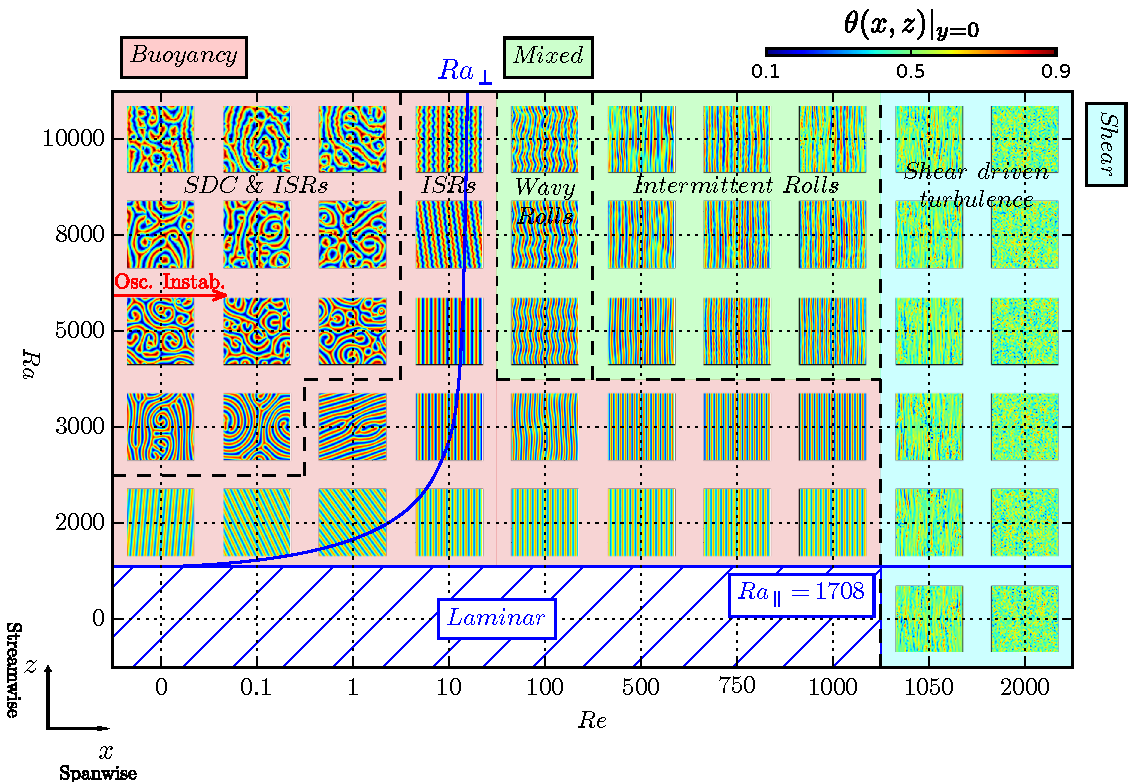
\includegraphics[width=0.9\textwidth]{TransitionalRBP/Figures/PhaseSpace/RaRePhaseSpace.pdf}
    \caption{The $Ra-Re$ phase space illustrates the terminal midplane temperature snapshots, $\theta(x,z)|_{y=0}$ for $Re \in [0,2000]$ and $Ra \in [0, 10000]$, classified into five distinct regimes: (1) SDC \& ISRs, (2) ISRs, (3) wavy rolls, (4) intermittent rolls and (5) shear-driven turbulence. The blue solid curves refer to primary neutral curves of the longitudinal and transverse rolls $Ra_\parallel, Ra_\perp$. The red curve refers to secondary oscillatory instability of ISRs at $Re = 0$ \citep{bodenschatz_recent_2000}. Shades of red, green and blue indicate their dominant mechanism, whether driven by buoyancy or shear (or mixed). The plot is not to scale.}
    \label{fig:rarephase}
\end{figure}

We present the results obtained from the DNS of transitional RBP flows, focusing on the parameter space defined by Rayleigh numbers in the range $Ra \in [0, 10000]$, and Reynolds numbers in the range of $Re \in [0, 2000]$ (see Appendix \ref{app:params} for the full details).
At the two end points of the $Re$-spectrum considered (i.e. $Re = 0, 2000$), SDC and subcritical shear-driven turbulence appear.
Figure \ref{fig:rarephase} shows the snapshots of the midplane temperature, $\theta(x,z)|_{y=0}$, of different flow regimes on the $Ra$-$Re$ phase space.
The solid blue curves represents to the neutral stability boundaries for the longitudinal and transverse rolls as $Ra_\parallel = 1708$ and $Ra_\perp = f(Re)$, respectively \citep{gage_stability_1968}.
In the absence of shear at $Re=0$, these curves merge into the classical critical RBC instability at $Ra_{c} = 1708$, as ISRs become rotationally invariant about the wall-normal axis.
Furthermore, a red arrow roughly indicates the secondary neutral stability boundary, marking the onset of oscillatory instabilities of ISRs within $5000 < Ra < 8000$ at $Re = 0$ \citep{clever_transition_1974}.
We note that the phase diagram in figure \ref{fig:rarephase} is not plotted to scale precisely but serves as a conceptual reference to distinugish between different flow states.

In this $Ra$-$Re$ phase space, we categorise the flow behaviour into five distinct regimes: (1) bistability between SDC and ISRs (SDC \& ISRs), (2) ideal straight rolls (ISRs), (3) wavy rolls, (4) intermittent rolls, and (5) shear-driven turbulence.
The categories are defined based on common flow structures (patterns), and/or dynamical characteristics, ranging from equilibrium solutions to intermittent and chaotic dynamics.
Furthermore, we classify these states based on their first and second-order statistical properties, where they appear independent of $Re$ in the buoyancy-dominated regime (shaded in red), and $Ra$ in the shear-dominated regime (shaded in blue), discussed in Appendix \ref{app:statistics}.
In the mixed regime shaded in green, both $Ra$ and $Re$ are important.
% The mixed regime flows (green shading), where both $Ra$ and $Re$ influence the statistics significantly (see Appendix \ref{app:statistics}).

In the buoyancy-dominated regime, the flow structures are predominantly organised by convection rolls, such as SDC, transverse, oblique, longitudinal rolls (and ISRs with no mean flow), or oscillatory rolls.
The bistability between SDC and ISRs is preserved for $Ra \geq 3000$ at $Re = 0.1$, and $Re = 1$ for $Ra \geq 5000$.
This points towards the existence of $Re$, at which SDC disappears, say $Re_s$, 
$Re_s$ appears to depend on $Ra$, as demarcated by the black dashed lines on the left side of figure \ref{fig:rarephase}.
However, computing this $Re_s$-threshold is beyond the scope of this thesis.

Notably, a transverse roll with a `hooked-like' defect is observed at $Re = 1$, $Ra = 3000$, reminiscent of the multiple `non-ISR' states in RBC (see references in \S \ref{sec:bkgrd_RBC}).
At $Re = 10$, SDC disappears and longitudinal rolls appear.
As $Re$ is increased further to $1000$, the longitudinal rolls emerge as the preferred solution at $Ra = 2000, 3000$.
% Indeed, the growth rates for the onset of longitudinal rolls become dominant compared to those of oblique/transverse rolls as $Re$ is increased \citep{gage_Reid_1968}.
Notably, the non-dimensionalised spanwise wavenumber of these longitudinal rolls is approximately $\alpha d \approx 1.65$, which happens to lie outside of the stability boundaries of the Busse balloon in RBC \citep{busse_non-linear_1978}.
This suggests that the stability boundaries of the longitudinal rolls may expand as $Re$ increases.
% Further evidence comes from the skewed-varicose longitudinal roll structure at $Re = 100$, $Ra = 3000$, which resembles a skewed-varicose instability, a secondary instability related to the Busse balloon boundaries \citep{Busse_Clever_1979}.

As $Re$ approaches $100$, the longitudinal rolls undergo a secondary wavy instability \citep{clever_instabilities_1991, pabiou_wavy_2005, nicolas_characterisation_2010}, leading to the emergence of wavy longitudinal rolls depicted in figure \ref{fig:rarephase}.
The wavelength of the streamwise waviness and the spanwise periodic longitudinal roll appear to be approximately three intervals of streamwise length, $\Lambda_z \sim L_z / 3$, and twelve intervals of spanwise length, $\Lambda_x \sim L_x/12$, respectively.
The ratio between the wavelength of streamwise waviness and spanwise roll is about $\sim 4$, around the ballpark reported by \cite{clever_instabilities_1991}.

% \begin{figure}
%     \centering
%     \includegraphics[width=\linewidth]{TransitionalRBP/Figures/PhaseSpace/theta_hat-compiled.pdf}
%     \caption{The time-averaged spatial planar $x$-$z$ wavenumber spectra of midplane perturbation temperature, $\frac{1}{T} \sum_T |\widehat{\theta'|_{y=0}}(n_x,n_z,t)|$ at $Re = 100,10$, (a,e) $Ra = 3000$, (b,f) $Ra = 5000$, (c,g) $Ra = 8000$, (d,h) $Ra = 10000$. The coefficient is defined by taking the Fourier transform of the instanteneous midplane perturbation temperature $\widehat{\theta'|_{y=0}}(n_x,n_z,t) = \int_{x,z} \theta'|_{y=0}(x,z,t) e^{-i(\alpha n_x x + \beta n_z z)} \; \mathrm{d}x \mathrm{d}z$ where $\alpha = 2\pi/L_x$ and $\beta = 2\pi/L_z$. The coefficients obey the conjugate symmetry, i.e $\widehat{\theta'|_{y=0}}(n_x,n_z,t)=\widehat{\theta'|_{y=0}}^*(-n_x,-n_z,t)$}
%     \label{fig:rollspectra}
% \end{figure}

\subsection{Spatiotemporal intermittent rolls}\label{sec:intermittentrolls}
\begin{figure}
    \centering
    \includegraphics[width=\linewidth]{TransitionalRBP/Figures/PhaseSpace/Ra8000-Re500-BotSpaceTime-TimeHist.pdf}
    \caption{The intermittent rolls regime at $Ra = 8000, Re = 500$, $t \in [0, 10000]$. The time history of (a) Nusselt number, and shear, (b) near-wall wall-normal and spanwise perturbation kinetic energy, (c) midplane temperature spacetime plot, and their corresponding near-wall and midplane temporal planar snapshots at (d,e) $t = 3736$, (f,g) $t = 6189$, and (h,i) $t = 8680$.}
    \label{fig:Ra8k-Re500-IntRolls}
\end{figure}

As $Re$ approaches $Re = 500$, the wavy rolls disappear.
Instead, a new regime, referred to as intermittent rolls, is observed.
In this regime, the longitudinal rolls remain as the dominant convection structure, interspersed with a spatio-temporal intermittent breakdown towards the laminar state.
For $Ra = 8000, Re = 500$, this behaviour is illustrated with figure \ref{fig:Ra8k-Re500-IntRolls}(a), where the temporal oscillations of the as the plane-averaged shear rate on the lower wall, $\langle \mathrm{d}w/\mathrm{d}y|_{y=-1} \rangle_{x,z} $, and the Nusselt number, $Nu$.
We note that the plane-averaged shear rate and Nusselt number for the laminar state is at 2 and 1 respectively. 

The spatio-temporal intermittent breakdown of the longitudinal rolls towards the laminar state is observed in figure \ref{fig:Ra8k-Re500-IntRolls}(b), where the bright and dark regions in the space-time plot of near-wall spanwise and wall-normal perturbation kinetic energy, $\mathcal{E}_{u'+v'} = 1/2\left[ u'|_{(y^+,z)=(15,8\pi)}^2 + v'|_{(y^+,z)=(15,8\pi)}^2 \right]$ (where $\mathbf{u}' = \mathbf{u} - W_{lam}(y)$, $y^+ = u_\tau y_0 / \nu$, $u_\tau = \sqrt{\langle \gamma/h \rangle_{t}}$, $y_0 = h - y = 0.44$,  refer to perturbation velocities, dimensionless height, frictional velocity, wall-normal height respectively), highlight the presence of longitudinal rolls and spatially-localised laminar states.
A similar obserbation is made with the space-time plot of midplane temperature, $\theta|_{(y,z)=(0,8\pi)}$, where elongated red/blue lines correspond to regions of longitudinal rolls, while green spots indicate spatially-localised laminar states, highlighting the breakdown process.
The near-wall transport properties, such as the Nusselt number and shear, exhibit strong correlations, peaking at $t = 3736$, corresponding to a spatially coherent longitudinal roll structure in figure \ref{fig:Ra8k-Re500-IntRolls}(d,e).
This is followed by a dip at $t = 6189$ and $t=8680$, indicative of the breakdown towards the laminar state shown in figures \ref{fig:Ra8k-Re500-IntRolls}(f,g) and \ref{fig:Ra8k-Re500-IntRolls}(h,i) respectively.
In other words, the longitudinal rolls enhance heat and momentum transfer across the wall, which is briefly disrupted by its breakdown towards the laminar state.
However, exploring the spatiotemporal intermittency of this regime remains challenging in a large extended domain, 
To overcome this challenge, we consider a confined domain, $\Gamma = \pi / 2$, where spatial intermittency could be artificially suppressed and discuss its temporal intermittent dynamics in \S \ref{sec:IntConfined}.

\subsection{Coexistence with turbulent bands}\label{sec:rbp_3.3}
\begin{figure}
    \centering
    \includegraphics[width=\linewidth]{TransitionalRBP/Figures/RaEffectOnTurbulence/Ra0-Re1050-3-BotSpaceTime-Lows.pdf}
    \caption{Shear-driven turbulence regime at $Ra = 0, Re = 1050$, $t \in [0, 8000]$. Spacetime plots of (a) near-wall wall-normal and spanwise perturbation kinetic energy, (b) midplane temperature spacetime plot, and near-wall and midplane temporal planar snapshots at (c,d) $t = 1100$, (e,f) $t = 4491$, and (g,h) $t = 6171$, highlighting a prolonged laminar patch.}
    \label{fig:spacetime-Ra0k-Re1.05k}
\end{figure}
As $Re$ approaches $Re = 1050$, shear-driven turbulence emerges as spatiotemporal intermittent turbulent-laminar bands, where turbulent and laminar regions can coexist (see references in \S \ref{sec:bkgrd_transitional}).
In the absence of buoyancy ($Ra = 0$), these bands emerge clearly, as shown in figure \ref{fig:spacetime-Ra0k-Re1.05k}.
The spacetime plot of the near-wall wall-normal and spanwise perturbation kinetic energy, $\mathcal{E}_{u'+v'}$, in figure \ref{fig:spacetime-Ra0k-Re1.05k}(a) highlights this coexistence, where the turbulent and laminar regions are indicated by dark and bright areas, respectively.
Notably, a period of prolonged laminar state is observed at $t = 1100, 4491, 6171$, represented by localised green regions in the midplane temperature spacetime plot, $\theta|_{(y,z)=(0,8\pi)}$, in figure \ref{fig:spacetime-Ra0k-Re1.05k}(b).
The prolonged laminar states are also evident in the near-wall and midplane temporal snapshots of figures \ref{fig:spacetime-Ra0k-Re1.05k}(c-h), shown as large pockets of dark and green regions filling approximately half of the spatial domain.
Next, we consider the influence of buoyancy on the turbulent-laminar bands and compare cases at $Ra = 0$ and $Ra = 10000$ at $Re = 1050$.
% The impact of $Ra$ on the nature of turbulent-laminar bands remains unclear.
% For instance, do longitudinal rolls emerge within laminar bands at $Ra > Ra_\parallel$?
% The emergence of longitudinal rolls suggests potential interactions and/or coexistence with neighbouring turbulent bands.
% In this section, we focus on the impact of $Ra$ on turbulent-laminar bands at $Re = 1050$, close to the subcritical shear-driven transition $Re$ for turbulence (see figure \ref{fig:rarephase}).
% We explore the role of longitudinal rolls, and their impact on turbulent-laminar bands, i.e. do longitudinal rolls appear within laminar bands at $Ra > Ra_{\parallel}$ and do they coexist with turbulent bands?
% We compare two numerical experiments, $Ra = 10000, 0$ at $Re = 1050$.
% We present the spacetime graph of the near-wall wall-normal and spanwise perturbation kinetic energy,$\frac{1}{2W_c}|u'+ v'|_{(y^+, z) = (15,8\pi)}$, and midplane temperature plots, $\theta(x,t)|_{y=0}$, and 3 pairs of $x-z$ planar snapshots at different times for $Ra = 10000, 0$, $Ra = 1050$ in figures \ref{fig:spacetime-Ra10k-Re1.05k} and \ref{fig:spacetime-Ra0k-Re1.05k} respectively.
\begin{figure}
    \centering
    \includegraphics[width=\linewidth]{TransitionalRBP/Figures/RaEffectOnTurbulence/Ra10000-Re1050-BotSpaceTime-Highs.pdf}
    \caption{Shear-driven turbulence regime at $Ra = 100000, Re = 1050$, $t \in [0, 8000]$. Spacetime plots of (a) near-wall wall-normal and spanwise perturbation kinetic energy, (b) midplane temperature spacetime plot, and their corresponding near-wall and midplane temporal $x-z$ planar snapshots at (c,d) $t = 1282$, (e,f) $t = 5077$, and (g,h) $t = 6358$, highlighting the coexistence of longitudinal rolls and turbulent bands.}
    \label{fig:spacetime-Ra10k-Re1.05k}
\end{figure}
At $Ra = 10000$, the features of the turbulent-laminar bands appearing as alternate dark and bright bands are visually consistent in the spacetime plot of near-wall wall-normal and spanwise perturbation kinetic energy, $\mathcal{E}_{u'+v'}$, in figure \ref{fig:spacetime-Ra10k-Re1.05k}(a).
% The near-wall wall-normal and spanwise perturbation kinetic energy in the spacetime plot for $Ra = 10000$ in figure \ref{fig:spacetime-Ra10k-Re1.05k}(a) exhibits similar turbulent-laminar band structures
However, key differences between the $Ra = 0$ case emerge.
Notably, the midplane temperature snapshots, $\theta|_{(y,z)=(0,8\pi)}$, at $t = 1282, 5077, 6358$ in figures \ref{fig:spacetime-Ra10k-Re1.05k}(d,f,g) reveal localised regions of streamwise-aligned red and blue stripes, indicating the presence of longitudinal rolls, which are absent in $Ra = 0$.
These longitudinal roll regions are located next to neighbouring turbulent (bright) regions in the near-wall perturbation kinetic energy snapshots in figures \ref{fig:spacetime-Ra10k-Re1.05k}(c,e,g), suggesting that longitudinal rolls coexist with turbulent patches at $Ra = 10000$.
However, we caution that similar red and blue stripes are also observed in $Ra = 0$, where longitudinal rolls are not expected, likely suggesting the presence of quasi-streamwise rollers, shown in figure \ref{fig:spacetime-Ra0k-Re1.05k}(f).
Nonetheless, turbulence occurs more spatially intermittently at $Ra = 0$, containing prolonged pockets of laminar regions, while the turbulent-laminar bands at $Ra = 10000$ appear more visibly consistently (compare figures \ref{fig:spacetime-Ra0k-Re1.05k}(a) and \ref{fig:spacetime-Ra10k-Re1.05k}(a)).
In other words, the presence of longitudinal rolls may promote turbulence locally, where prolonged regions of laminar patches do not appear.
However, investigating this remains challenging due to the spatiotemporal nature of a large extended domain.
To address this, we focus our analysis to a confined domain, $\Gamma = \pi / 2$, where turbulent bands and longitudinal bands cannot coexist, thereby reducing spatial intermittency discussed further in \S \ref{sec:4}.

% This suggests that longitudinal rolls, emerging from the linearly unstable laminar state, might play a role in sustaining turbulence.
% At $Ra = 0$, the turbulent-laminar bands appear more spatially intermittent, where prolonged regions of localised non-turbulent patches emerge near $t = 1100, 6171$, shown as dark and green patches in figures \ref{fig:spacetime-Ra0k-Re1.05k}(a,b).
% Due to the spatial-temporal complexity of the coexistence between longitudinal rolls and turbulence at $Ra = 10000$, it may be challenging to establish connections between them.
% As such, we consider investigate the dynamics within an MFU, where longitudinal rolls and turbulence could be spatially localised.
% For instance, do longitudinal rolls transition to turbulence locally?
% In the  alised regions of alternating elongated hot (red) and cold (blue) stripes within $tU_c/h \in (1400, 1500)$, $x \in (6\pi, 10\pi)$ and $tU_c/h \in (1500, 2000)$, $x \in (0, 4\pi)$ in the midplane temperature spacetime plots of figures \ref{fig:spacetime-Ra10k-Re1.05k}(b) and \ref{fig:spacetime-Ra2k-Re1.05k}(b) respectively, hinting at the presence of longitudinal rolls.
% These elongated hot and cold stripes along the midplane are not to be confused with turbulent streaks which reside near the wall.
% Indeed, we observe patches of longitudinal rolls from the midplane temperature snapshots of figures \ref{fig:spacetime-Ra10k-Re1.05k}(d,f,h) and \ref{fig:spacetime-Ra2k-Re1.05k}(d,f,h), visually differing from the snapshots of $Re = 1800$ (compare with figures \ref{fig:spacetime-Ra10k-Re1.8k}(d,f,h) and \ref{fig:spacetime-Ra2k-Re1.8k}(d,f,h)).
% Interestingly, the longitudinal rolls appear spatially localised, co-existing with neighbouring patches of spatially localised turbulence, consistent in both simulations.
% A subtle difference between the simulations lies in the `uniformity' of the turbulent-laminar bands. 

% For $Ra = 10000$, the turbulent bands appear spatially and temporally uniform, repeating in regular intervals.
% However, at $Ra = 2000$, the turbulent-laminar bands appear to be less uniform, with a prolonged laminar (darkened) patch within $tU_c/h \in (2000, 2500), x \in (6\pi, 8\pi)$ (see figures \ref{fig:spacetime-Ra2k-Re1.05k}(a,b) and the snapshot at $tU_c/h = 2250$ in figures \ref{fig:spacetime-Ra2k-Re1.05k}(g,h)).
% Furthermore, we consider simulations with $Ra = 10000, 0$, where the onset of longitudinal rolls could be precisely controlled.

\section{The role of longitudinal rolls}\label{sec:rbp_4}
\subsection{The thermally-assisted sustaining process (TASP) in a confined domain}\label{sec:TASP}
\begin{figure}
    \centering
    \includegraphics[width=\linewidth]{TransitionalRBP/Figures/RaEffectOnTurbulence/Ra10000-Re1050-MidBotTimeHist.png}
    \caption{Intermittent dynamics in a confined domain at $Ra = 10000$, $Re = 1050$, $t\in[0,3000]$, $\Gamma = \pi/2$. The time history of the (a) Nusselt number and shear. Temporal snapshots of volumetric temperature, planar near-wall streamwise and spanwise perturbations at (b) $t = 1291.5$, (c) $t = 1480.5$, (d) $t = 1564.5$, (e) $t = 1711.5$. Longitudinal rolls and transient turbulence are observed at (b,d) and (c,e), respectively.}
    \label{fig:Ra10k-Re1050-small}
\end{figure}

Motivated by the minimal flow unit (MFU) approach to study turbulence \citep{jimenez_moin_1991}, we consider simulations confined to a confined domain defined by $\Gamma = \pi/2$, where the longitudinal rolls and localised turbulence could be spatially isolated.
We first consider a numerical simulation at $Ra = 10000, Re=1050$, in $\Gamma = \pi/2$, time integrated for $t \in [0, 3000]$.
The initial condition has been sampled from a statistically stationary turbulent field at $Re = 2000$, which is then lowered slowly to $Re = 1050$.
The time history from $t \in [0, 3000]$ of the near-wall transport properties such as the Nusselt number, $Nu$, shear, $\langle \mathrm{d}w/\mathrm{d}y|_{y=-h}\rangle_{x,z}$, volumetric temperature, $\theta(\mathbf{x})$, and near-wall streamwise and spanwise perturbation velocities snapshots, $w'|_{y^+= 15}, v'|_{y^+=15}$, are presented in figure \ref{fig:Ra10k-Re1050-small}.
In this confined domain, the dynamics of the system exhibit temporal intermittency, where the solution trajectory appears to wander between the longitudinal rolls and turbulent dynamics, marked by high and low near-wall transport properties, respectively.
The turbulent dynamics mentioned here refer to chaotic trajectories (see \S \ref{sec:PPF}) marked by a disordered volumetric temperature field and high near-wall transport quantities.

Starting from a longitudinal roll state of spanwise wavenumber of $\alpha d = 4$ at $t = 1291.5$ in figure \ref{fig:Ra10k-Re1050-small}(b), the solution erupts into turbulence at $t = 1480.5$, marked by a disordered temperature field in figure \ref{fig:Ra10k-Re1050-small}(c).
During this breakdown, the near-wall snapshots of streamwise perturbation velocity, $w'|_{y^+ = 15}$, and wall-normal perturbation velocity, $v'|_{y^+ = 15}$, illustrated in the bottom panels of figures \ref{fig:Ra10k-Re1050-small}(c), reveal three pairs of high- and low-speed streaks, each with an average spanwise wavelength of $\Lambda_x^+ \approx 339/3 = 113$ (where $\Lambda_x^+ = u_\tau \Lambda_x / \nu$ refers to non-dimensionalised wavelength), close to the mean streak spacing ($\Lambda^+ \sim 100$) commonly reported in shear flow turbulence \citep{kline_1967,Smith_1983,Kim_Moin_Moser_1987,hkw_1995}.
These streaks appear to be meandering, negatively correlated with wall-normal perturbation velocities, reminiscent of a streak breakdown process \citep{hkw_1995}, or a bursting event \citep{Kim_Kline_Reynolds_1971}, where high- and low-speed streaks are brought close to and away from the wall, respectively, enhancing near-wall transport quantities.
Indeed, this is reflected by large increments of the Nusselt number and shear of roughly $40\%$ at $t = 1480.5$ in figure \ref{fig:Ra10k-Re1050-small}(a).
Subsequently, the solution trajectory returns to a longitudinal roll state at $t=1564.5$, before erupting into turbulence at $t = 1711.5$ (see figures \ref{fig:Ra10k-Re1050-small}(d,e) respectively).
This suggests that the turbulence has a finite lifetime, occurring transiently before decaying towards the laminar state at $Re = 1050$ \citep{hof_2006, schneider_2007}, which is linearly unstable, leading to the onset of longitudinal rolls where transient turbulence could be re-excited again.
% It is likely that this temporal intermittency, described by the oscillation between turbulent dynamics and the longitudinal rolls, occurs as an intrinsic dynamical state in $Ra = 10000, Re = 1050$, when confined to $\Gamma = \pi / 2$.
% Inspired by the lift-up effect as a mechanism to sustain turbulence \citep{brandt2014lift}, we suggest that the longitudinal rolls could redistribute the streamwise mean momentum, providing an alternate mechanism towards turbulence.
% However, turbulence appears to have a finite lifetime, before decaying into longitudinal rolls where a cycle between longitudinal rolls and turbulence could be observed.
% In this case, we hypothesize that the longitudinal rolls at $Ra = 10000$ promote a mechanism for transition to turbulence, in which turbulence may not be sustained at $Re = 1050$ independe , ultimately decaying into the laminar state where the longitudinal rolls are then excited again, forming a thermally-sustaining turbulent mechanism.

\begin{figure}
    \centering
    \includegraphics[width=\linewidth]{TransitionalRBP/Figures/RaEffectOnTurbulence/Ra0-Re1050-MidBotTimeHist.png}
    \caption{Relaminarisation in a confined domain at $Ra = 0$, $Re = 1050$, $t\in[0,3000]$, $\Gamma = \pi/2$. The time history of the (a) Nusselt number and shear. Temporal snapshots of volumetric temperature at (b) $t = 31.5$, (c) $t = 63$, (d) $t = 157.5$, (e) $t = 672$.}
    \label{fig:Ra0k-Re1050-small}
\end{figure}

To test this hypothesis, we consider a numerical simulation at $Ra = 0$, $Re = 1050$, in $\Gamma = \pi / 2$, where longitudinal rolls cannot appear.
The initial condition is taken from a stationary turbulent solution at $Ra = 0$, $Re = 2000$, which is then lowered slowly to $Re = 1050$, and then time integrated for $t \in [0, 700]$.
The time history of Nusselt number, $Nu$, shear, $\langle \mathrm{d}w/\mathrm{d}y|_{y=-h}\rangle_{x,z}$, and the volumetric temperature snapshots, $\theta(\mathbf{x})$, are reported in figure \ref{fig:Ra0k-Re1050-small}.
% Starting from $t = 31.5$, a localised patch of turbulence appears in $x^+,z^+ \in [0, 164]$ in figure \ref{fig:Ra0k-Re1050-small}(c), the turbulent patch subsequently decays, ultimately settling into a laminar state at $t = 630$ in figure \ref{fig:Ra0k-Re1050-small}(e).
Turbulence occurs transiently, which decays towards the laminar solution in $t \in [0, 700]$ within the confined domain.
As we compare the results between $Ra = 0$ and $Ra = 10000$, we propose that the longitudinal rolls at $Ra= 10000$ could provide a transition mechanism towards transient turbulence, which could be sustained indefinitely.

\begin{figure}
    \centering
    \includegraphics[width=\linewidth]{TransitionalRBP/Figures/RaEffectOnTurbulence/T1620-MidBotTimeHist-Quenched-Annotated.pdf}
    \caption{$Ra$-quenching experiments for $Ra = 8000, 5000, 3000, 2000$, $Re = 1050$, $\Gamma = \pi/2$, $t \in [850.5, 5000]$. The time history of (a) shear and (b) volumetric temperature snapshots of the initial condition at $t = 850.5$. Volumetric temperature snapshots for $Ra = 8000$ at (c,d) $t = 1312.5, 1743$, and $Ra = 5000$ at (e,f) $t = 1312.5, 3570$, revealing a longitudinal roll and a turbulent state, respectively. Stable longitudinal rolls emerge for $Ra = 3000$ at (g,h) $t = 1312.5, 4200$, and $Ra = 2000$ at (j,k) $t = 1312.5, 4200$.}
    \label{fig:RaQuench}
\end{figure}
% While, we have only considered the end cases of $Ra = 10000,0$ and the impact of the range of $Ra \in (0, 10000$ on this transition mechanism remains unclear.
% For instance, there could be a critical $Ra > Ra_{c,sec}$ which transition occurs.
% To investigate this further, we performed four numerical experiments in which an initial condition is taken at $Ra = 10000, Re = 1050$, $tU_c/h = 850.5$ (see figure \ref{fig:Ra10k-Re1050-small}, before the onset of longitudinal rolls) whereby $Ra$ is instantly reduced from $Ra = 10000$ to $Ra = 8000, 5000, 3000,2000$.

Next, we investigate the impact of longitudinal rolls on this proposed mechanism at different $Ra$.
We perform four numerical simulations with an initial condition taken from $Ra = 10000, Re = 1050$, at $t = 850.5$ (before the onset of longitudinal rolls, see figure \ref{fig:Ra10k-Re1050-small}), which is lowered instantaneously to $Ra = 8000, 5000, 3000, 2000$ respectively.
The initial conditions are time-integrated further to $t \in [850.5, 5000]$, and the time history of the shear, $\langle \mathrm{d}w/\mathrm{d}y|_{y=-h}\rangle_{x,z}$, and the temperature volumetric temporal snapshots, $\theta(\mathbf{x})$, of these `Ra-quenching' experiment are presented in figure \ref{fig:RaQuench}.
The time history of shear is visibly intermittent for $Ra = 8000, 5000$, depicted as the orange and green trajectories in figure \ref{fig:RaQuench}(a), similar to $Ra = 10000$.
At $Ra= 8000, 5000$, the longitudinal rolls emerge at $t = 1312.5$ (see figures \ref{fig:RaQuench}(d,f)), before erupting into turbulence at $t = 1743$ and $t = 3570$ in figures \ref{fig:RaQuench}(e,g) respectively.
This is then accompanied by a large spike in the near-wall transport properties before dipping briefly in figure \ref{fig:RaQuench}(a).
As $Ra$ is lowered to $Ra = 3000, 2000$, the transients begin to decay into a longitudinal state from $t = 850.5$ to $t = 1312.5$, which remains asymptotically stable until $t = 4200$, represented as the red and purple trajectories of figures \ref{fig:RaQuench}(i,k) respectively. 
This suggests that the longitudinal rolls become linearly unstable for $Ra = 8000, 5000$, leading to turbulence, while remaining stable for $Ra = 3000,2000$.
Notably, the longitudinal rolls state at $Ra = 5000$ remained saturated over a longer period $t \in [1500, 3400]$ (green curve of figure \ref{fig:RaQuench}), suggesting an underlying linear instability with a smaller growth rate compared to $Ra =  8000$.
We note that the longitudinal rolls in figure \ref{fig:RaQuench} have a spanwise wavenumber of $\alpha d=4$, which corresponds to the wavenumber of the dominant primary instability (see Appendix \ref{app:long-pri}), indicating that it is the preferred wavenumber within the confined domain.

% This suggests a critical $Ra$ within $Ra \in (3000,5000)$ where the longitudinal rolls become linear unstable.
% Compared to $Ra = 8000, 10000$, the quiescent region of $Ra =5000$, extends over a visibly longer period $tW_c/h \in (1500, 3400)$ (green curve of figures \ref{fig:RaQuench}), landing support for different perturbation growth rates arising from linear instability.
% The results likely point towards a possible critical $Ra_{c,sec}$, where longitudinal rolls may become linearly unstable, subsequently transitioning into turbulence for $Ra > Ra_{c,sec}$.

\begin{figure}
    \centering
    \includegraphics[width=\linewidth]{TransitionalRBP/Figures/RaEffectOnTurbulence/ev-compiled.pdf}
    \caption{The growth rates of infinitesimal perturbations linearised about longitudinal rolls, $\mathbf{q}_{LR}$, of spanwise wavenumber of $\alpha d = 4$, against (a) streamwise wavenumber $\lambda$, and (b) $Ra$ for $\beta d =1$. The hatches in (a) refer to wavenumbers smaller than those admissible in $\Gamma = \pi/2$. The dash-dotted line in (b) is a standard quadratic regression yielding $Ra_{s}\approx 4720$.}
    \label{fig:SecStabLongRolls}
\end{figure}

To determine the stability characteristics of the longitudinal rolls, we perform linear stability analysis about the longitudinal roll state ($\alpha d= 4$), at $Ra = 10000, 8000, 5000, 3000, 2000$.
The details of linear stability analysis are described in \S\ref{sec:linearstab}, where $\lambda$ and $\mathbf{\hat{s}_\beta}e^{i\beta z}$ refer to the eigenvalue and eigenmode.
The longitudinal roll (base) states, $\mathbf{q}_{LR}$, are obtained by time integrating an initial condition consisting of the laminar (conduction) state, superimposed by the primary eigenmode, $\alpha d = 4$, at $Ra = 10000, 8000, 5000, 3000, 2000$, in a two-dimensional $x-y$ plane, suppressing any three-dimensional perturbations numerically.
The growth rates as a function of discrete streamwise wavenumbers, $2 \leq \beta d \leq 5$, are presented in figure \ref{fig:SecStabLongRolls}.
We note that the admissible streamwise wavenumbers within $\Gamma = \pi/2$ are $\beta d = m$, where $m$ is a positive even integer, $m = 2, 4, ..$, and $\beta d = 3, 5$ are included for completeness.
The longitudinal rolls are linearly unstable for $Ra \geq 5000$, while they remain stable for $Ra \leq 3000$, confirming our hypothesis earlier. 
Notably, the growth rates between $Ra = 5000$ and $Ra = 10000$ differ by an order of magnitude, which could explain the prolonged period of saturation in the green curve of figure \ref{fig:RaQuench}(a,b).
The dominant secondary instability of longitudinal rolls in $\Gamma = \pi / 2 $ has a streamwise wavenumber of $\beta d = 2$.
Using a standard quadratic regression, the critical Rayleigh number for disturbances with $\beta d = 2$ is approximately $Ra_{s} \approx 4720$, presented in figure \ref{fig:SecStabLongRolls}(b).

\begin{figure}
    \centering
    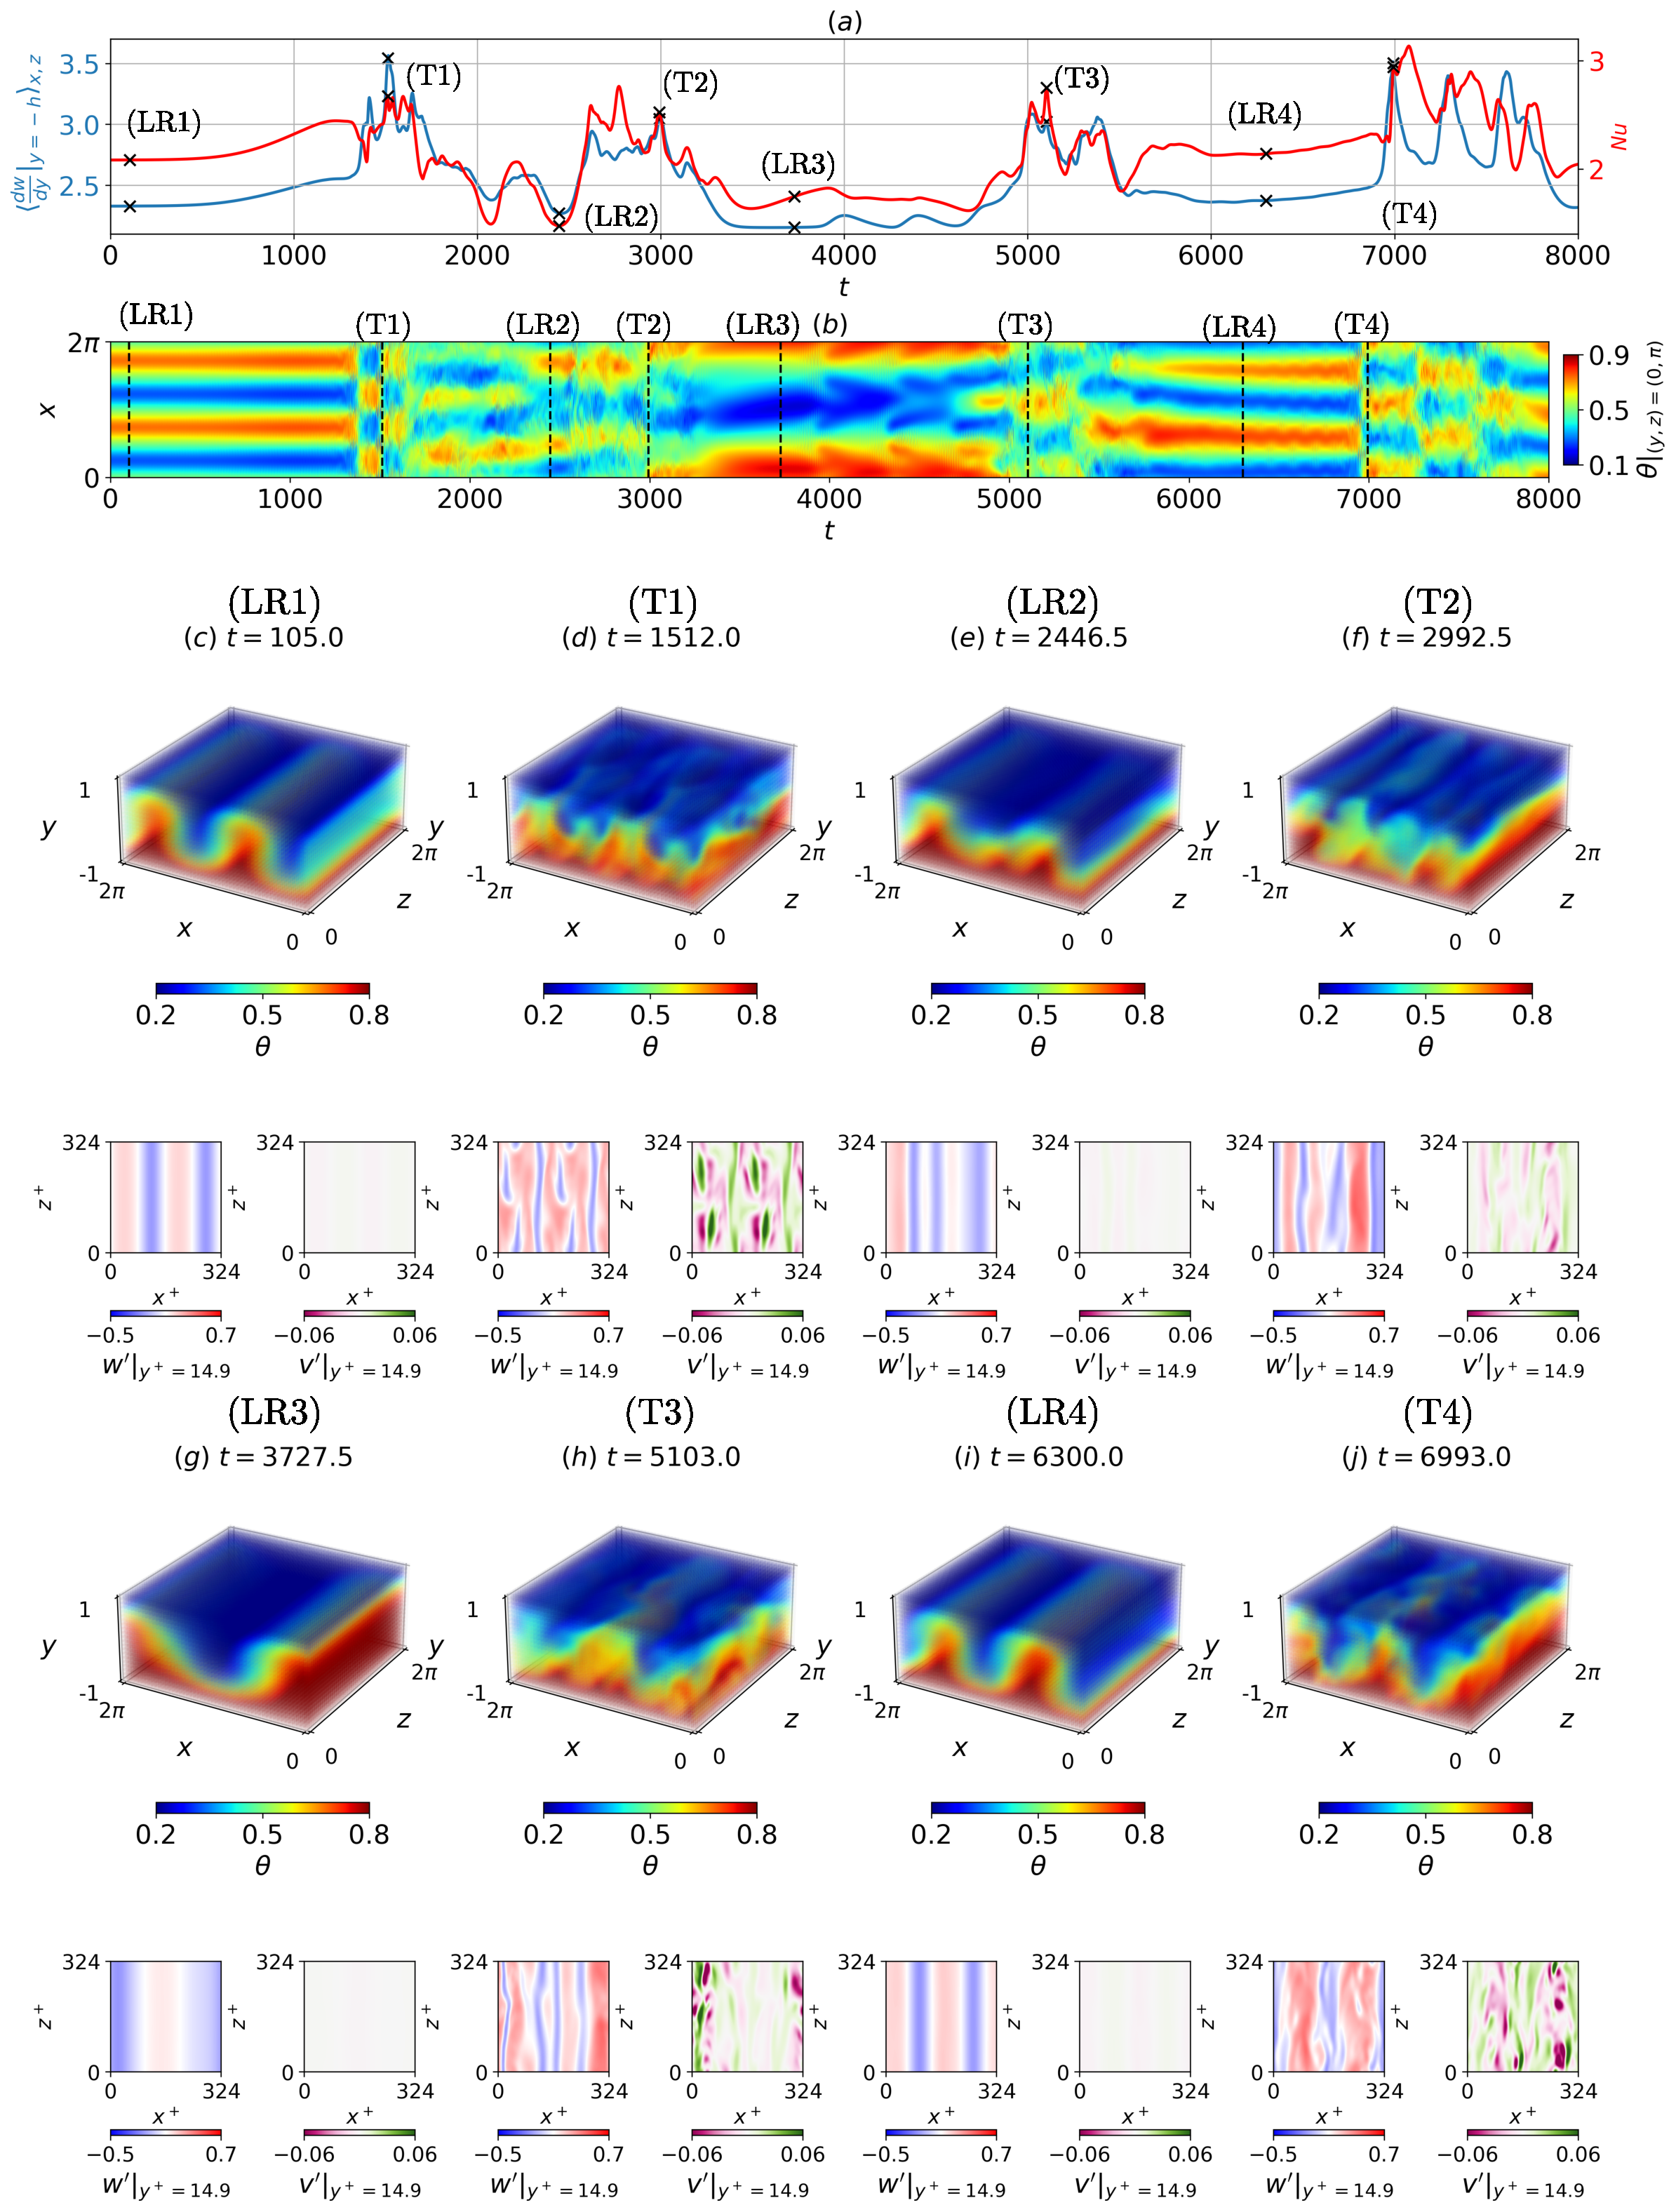
\includegraphics[width=\linewidth]{TransitionalRBP/Figures/RaEffectOnTurbulence/Ra5000-Re1050-MidBotTimeHist-PEig-labelled.pdf}
    \caption{Integrating along the dominant unstable manifold, $\beta d =2$, of the longitudinal rolls at $Ra = 5000, Re = 1050, \Gamma = \pi/2$, $t\in[0,8000]$. Time history of the (a) Nusselt number and shear, and (b) midplane temperature spacetime plot. This system oscillates between the longitudinal rolls ($LR1-4$) and turbulence ($T1-4$) over four intervals. Snapshots of volumetric temperature and near-wall streamwise and spanwise velocity perturbations at (b) $t = 105$, (c) $t = 1512$, (d) $t = 2446.5$, (e) $t = 2992.5$, (f) $t = 3727.5$, (g) $t = 5103$, (h) $t = 6300$, (i) $t = 6993$.}
    \label{fig:intermittent-dynamics}
\end{figure}

Following this, we examine the dominant unstable manifold ($\beta d = 2$) of the longitudinal rolls, by considering an initial condition,
\begin{equation}\label{eq:rbp_SecInstab}
    \mathbf{q}_0(\mathbf{x},t=0) = \mathbf{q}_{LR}(x,y) + \mathbf{\hat{q}}_\beta(x,y)e^{i\beta z},
\end{equation}
which is prescribed to equation \eqref{eq:rbp_RBP}. Here, $\hat{\mathbf{q}}_\beta e^{i\beta d z}$ is an eigenmode at $\beta d$, and the amplitude of which was scaled such that its total energy is defined by,
\begin{equation}\label{eq:rbp_totalenergy}
    \delta = \frac{1}{{V}} \int_\Omega \mathbf{\hat{u}}(\mathbf{x})^T\mathbf{\hat{u}}(\mathbf{x}) + \frac{Ra}{8Re^2Pr}\hat{\theta}(\mathbf{x})^2 \; \mathrm{d}\Omega \approx O(10^{-3})
\end{equation}
is considered.
We have also considered that $\delta = 10^{-2}, 10^{-4}$, where $\delta = 10^{-3}$  was found to be sufficiently small enough to ensure linear growth, while large enough to be computationally practical.

The initial condition is time integrated from $t \in [0, 8000]$, and its time history of near wall transport properties such as the Nusselt number, $Nu$ and shear, $\langle \mathrm{d}w/\mathrm{d}y|_{y=-h}\rangle_{x,z}$, midplane temperature spacetime plot, $\theta|_{(y,z)=(0,\pi)}$, volumetric temperature, $\theta(\mathbf{x})$, and near-wall streamwise and spanwise perturbation velocities snapshots, $w'|_{y^+= 15}, v'|_{y^+=15}$, are presented in figure \ref{fig:intermittent-dynamics}.
% To investigate whether the transition mechanism towards turbulence is due to this linear instability, we consider a numerical experiment along the dominant unstable manifold ($\beta d = 2$) of longitudinal rolls ($\alpha d = 4$).
% The initial condition consists of the dominant secondary eigenmode ($\beta d = 1$), superimposed by longitudinal rolls with streamwise wavenumber, $\alpha d =4$, at $Ra = 5000, Re= 1050$.
% Marked by several `quiescent' and large spikes in the $Nu$ and shear, the solution trajectory visits the longitudinal roll and turbulent states four times, shown as snapshots, labelled $LR1$ to $LR4$, and $T1$ to $T4$ respectively.
The intermittent trajectory is visually present, oscillating between the longitudinal rolls and transient turbulence over four cycles $t = [0, 8000]$, marked by regions of low and high near-wall transport quantities in figure \ref{fig:intermittent-dynamics}(a) and alternating between organised and disorganised longitudinal rolls in figure \ref{fig:intermittent-dynamics}(b).
The snapshots of figure \ref{fig:intermittent-dynamics} illustrate the volumetric temperature field, planar near-wall streamwise and wall-normal perturbations, resembling the longitudinal rolls ($LR1-4$), and transient turbulent states ($T1-4$).
As the solution emerges from the unstable manifold of the longitudinal roll state, $(LR1)$ in figure \ref{fig:intermittent-dynamics}(c), the trajectory erupts into turbulence at $t = 1512$, marked by a disordered volumetric temperature field with high- and low-speed streaks in snapshot $(T1)$ in figure \ref{fig:intermittent-dynamics}(c).
These high- and low-speed streaks are negatively spatially-correlated with wall-normal perturbation velocities in figure \ref{fig:intermittent-dynamics}(d), reminiscent of sweeps and ejection events commonly found in turbulent shear flows \citep{Wallace_1972, Willmarth_1972}.
Notably, the flow structures in snapshot $T1$ in figure \ref{fig:intermittent-dynamics}(d), appear visibly symmetric along the centerline of the channel, $x^+ \approx 162$ (where $x^+= u_\tau x/\nu$ refers to the non-dimensionalised spanwise coordinate), comparable to the invariant states identified in transition shear flows \citep{Waleffe_2001,kerswell2005,eckhardt2007,gibson2008,graham21}.
Turbulence occurs transiently, and the solution decays towards a longitudinal roll-liked state at $t = 2446.5$, shown by snapshot $(LR2)$ in figure \ref{fig:intermittent-dynamics}(e), thereby completing one single cycle.
We note that the snapshot $(LR2)$ does not strictly resemble the longitudinal roll state at snapshot $(LR1)$, however, we show that they are similar and reside close by in state space, as we shall see later.
The intermittent cycle repeats over three subsequent intervals, where the turbulent dynamics and longitudinal rolls emerge at $t = 2992.5, 5103, 6993$, and $t = 3727.5, 6300$, represented as snapshots $(T2,3,4)$ and $(LR3,4)$ in figures \ref{fig:intermittent-dynamics}(f,h,j) and \ref{fig:intermittent-dynamics}(g,i) respectively.

Here, we showed that the dominant unstable manifold of the longitudinal rolls is linked to turbulent dynamics, a transition mechanism based on linear instability.
Interestingly, a `single' longitudinal roll with $\alpha d = 2$ emerges after turbulence decays, shown as snapshot $(LR3)$.
This suggests that other unstable manifolds may be linked to the transition to transient turbulence.

\begin{figure}
    \centering
    \includegraphics[width=\linewidth]{TransitionalRBP/Figures/RaEffectOnTurbulence/Ra5000-Re1050-StateSpace-dudy.png}
    \caption{State space projection based on the planar averaged centerline velocity and shear, coloured by the volume normalised perturbation kinetic energy at $Ra = 5000$, $Re = 1050$, $\Gamma = \pi/2$, (a) $t \in[0,800]$, (b) $t \in [0, 68750]$.  The open black circles represent the unstable equilibria of longitudinal rolls and the laminar state. Note that the black-crosses, labelled by (T1-4) and (LR1-4), refer to temporal snapshots in figure \ref{fig:intermittent-dynamics}, not equilibria solutions.}
    \label{fig:intermittent-state-space}
\end{figure}

To visualise the temporal dynamics in figure \ref{fig:intermittent-dynamics} with better clarity, we project the solution trajectory onto state observables using the planar averaged centerline velocity, $\langle w|_{y=0} \rangle _{x,z}$, shear, $\langle \mathrm{d}w/\mathrm{d}y|_{y=-h}\rangle_{x,z}$ coloured by the volume normalised perturbation kinetic energy, $1/(2V)||\mathbf{u}'||^2$ , in figure \ref{fig:intermittent-state-space}.
These observables seek to distinguish the region of turbulent dynamics, longitudinal roll state, and laminar state residing in near $(0.82, 3.2)$, $(0.90, 2.32)$ and $(1, 2)$, respectively.
This separation is further supported by the location of the temporal snapshots between $(T1-4)$ and $(LR1-4)$, organised near the turbulent dynamics and in longitudinal roll state, $\mathbf{q}_{LR, \alpha d = 4}$, setting them apart.
% Notably, the turbulent dynamics are located near the top left corner, while the longitudinal roll and laminar states are situated at the bottom right corner.
We emphasise that the unstable longitudinal roll state, $\mathbf{q}_{LR, \alpha d = 4}$, and laminar states denoted by open circles are unstable equilibria, while the snapshots longitudinal roll, $(LR1-4)$, and turbulent snapshots, $(T1-4)$, denoted by black crosses, are not.

The solution trajectory emerges from the unstable manifold of the longitudinal rolls, $\mathbf{q}_{LR_{\alpha d = 4}}$, evolving towards turbulent dynamics around $(0.85,3.2)$, denoted by high shear.
Turbulence is transient, occurring with a finite lifetime \citep{hof_2006,schneider_2007}, eventually decaying towards the laminar state.
As the solution trajectory approaches the laminar solution $(1,2)$, it abruptly reverses towards the longitudinal roll state near $(0.95, 2.15)$, $(LR3)$.
Subsequently, the solution trajectory could depart along the unstable manifold of the longitudinal rolls again, leading to the onset of turbulence, where the cycle repeats.

To determine if this cycle could be sustained indefinitely, we consider a longer time horizon, $t \in [0, 68750]$, illustrated in figure \ref{fig:intermittent-state-space}(b).
The solution trajectory wanders between the `cloud' of chaotic transient turbulence at the top left corner (in red), and longitudinal roll and laminar state (in blue) in the bottom right, forming a basin of attraction between the unstable longitudinal rolls, transient turbulence and the laminar state.
We suggest that this basin of attraction, is likely established above a critical $Ra$ as the longitudinal rolls become linearly unstable (i.e $Ra \gtrsim Ra_{s} \approx 4720$, see figure \ref{fig:SecStabLongRolls}(b)), providing an intermediate pathway towards transient turbulence, which could be regenerated again - a `self-sustaining' dynamical process.
We refer to this sustaining process as the \emph{thermally-assisted sustaining process (TASP)}, inspired by the self-sustaining process (SSP) from turbulent shear flows \citep{hkw_1995}.

% The turbulence dynamics near the top left corner are reminiscent of a chaotic saddle in state space \citep{Kreilos_2012, zammert_2015}, where turbulence ultimately relaminarises.
% Over a longer period, the solution trajectory wanders between the `cloud' of turbulent dynamics near (0.85, 0.0035) and the longitudinal rolls near (0.95, 0.0015), distinguished by regions of high and low shear, highlighted as red and blue trajectories.
% We note that in several instances, as the solution trajectory approaches the laminar solution, it `u-turns' abruptly to either $\mathbf{q}_{LR,\alpha d = 2,4}$
% The trajectory emerges from the unstable manifold of the longitudinal rolls, erupting into finite lifetime turbulence which subsequently decays towards the laminar state, which quickly re-energises to the longitudinal rolls, forming a basin of attraction.
% Indeed, the solution trajectory oscillates between the turbulent chaotic saddle, laminar and longitudinal roll state continuously over a longer time horizon, $t \in [0, 68750]$, demonstrating this basin of attraction shown in figure \ref{fig:intermittent-state-space}(b).
% Perhaps this process can be extended to the intermittent regime, where the turbulent chaotic saddle disappears as $Re$ decreases towards $Re = 500$ (see figure \ref{fig:rarephase}), and a cycle between the longitudinal rolls and the laminar state remains, a characteristic of the intermittent role regime in figure \ref{fig:Ra8k-Re500-IntRolls}.
% As $Re$ increases past a threshold $Re$, turbulence is likely to be sustained, where the chaotic saddle stabilises into a chaotic attractor.
% In this case, the solution trajectories are likely to be confined to the chaotic attractor, without ever visiting the longitudinal rolls, and the statistics described by the chaotic attractor defined by $Re$ as in figure \ref{fig:sheardrivenstatistics} suggest.

\subsection{Variation of $Ra$ and $Re$ on the thermally sustained turbulent process within $\Gamma = \pi/ 2$}\label{sec:IntConfined}
\begin{figure}
    \centering
    \includegraphics[width=\linewidth]{TransitionalRBP/Figures/RaEffectOnTurbulence/ConsolidatedPlot-temporal.pdf}
    \caption{The behaviour of the unstable and stable longitudinal rolls at $Ra = 8000, 4000$ for (a,e) $Re = 600$, (b,f) $Re = 700$, (c,g) $Re = 1000$ and (d,h) $Re = 1400$ within $\Gamma = \pi/2$. Each parameter regime consist of three panels from the top to bottom, depicting the midplane temperature spacetime plot, $\theta|_{(y,z) = (0, \pi)}$, time history of the Nusselt number and shear, and state space projection based on the planar averaged centerline velocity and shear, coloured by the volume normalised perturbation kinetic energy.}
    \label{fig:dynamical-process}
\end{figure}
In this section, we explore the behaviour of the \emph{TASP} as $Re$ and $Ra$ are varied.
We consider eight different cases at $Ra = 8000, 4000$ and $Re = 600, 700, 1000, 1400$.
The results of these eight cases, where longitudinals rolls are either unstable at $Ra = 8000$ or stable at $Ra = 4000$, are shown in figure \ref{fig:dynamical-process}, depicting the spacetime plots of midplane temperature, $\theta|_{y=0}(x,t)$, time history of the Nusselt number, $Nu$, and shear, $\langle \mathrm{d}w/\mathrm{d}y|_{y=-h}\rangle_{x,z}$ and state space projection using the planar averaged centerline velocity, $\langle w|_{y=0} \rangle_{x,z}$, shear, coloured by the volume normalised perturbation kinetic energy, $\frac{1}{2V}||\mathbf{u'}||^2$.
For all cases except $Ra = 4000$, $Re = 1000$ and $Re = 1400$, their initial conditions are prepared from the laminar state, superimposed by a random noise based on a Gaussian distribution with zero mean and unit variance, scaled to a total energy of $\delta = 10^{-3}$ (see definition in equation \eqref{eq:rbp_totalenergy}).
For the exceptional cases at $Ra = 4000$, $Re = 1000$ and $Re = 1400$, where subcritical turbulence and stable longitudinal rolls are expected, their initial conditions are obtained by gradually lowering $Re$ from a statistically stationary turbulent solution at $Re = 2000$.
We note that we have not explicitly performed a linear stability analysis of the longitudinal rolls for the parameter regime in figure \ref{fig:dynamical-process}, however, they appear to be unstable at $Ra = 8000$, while being stable at $Ra = 4000$ from DNS.

At $Ra = 8000$, $Re = 1000$, $t \in [0, 10000]$ in figure \ref{fig:dynamical-process}(c), the trajectory visits the transient turbulent regime near $t=7200$, which decays towards the longitudinal roll state, $\mathbf{q}_{LR}$, at $t = 7400$, which could be regenerated again, consistent with the \emph{TASP} in \S \ref{sec:TASP}.
% As $Ra$ decreases to $4000$, the longitudinal rolls become linearly stable, emerging as an asymptotically stable state.
% To illustrate this, the initial condition at $Ra = 4000, Re = 1100$ (gradually lowered from $Re=2000$) is time-integrated for $t = [0, 1500]$ in figure \ref{fig:dynamical-process}(g).
% \To illustrate this case in figure \ref{fig:dynamical-process}(g), where the initial condition is taken from a statistically stationary turbulent state at $Re = 2000$, and then gradually lowered to $Re = 1100$.
% As $Ra$ is lowered to $4000$, the basin of attraction disappears in figure \ref{fig:dynamical-process}(g).
As $Ra$ is lowered to $4000$, the solution trajectory decays towards the longitudinal roll state, $\mathbf{q}_{LR}$, where the \emph{TASP} disappears.
In this case, the longitudinal rolls are linearly stable, confirming our hypothesis earlier that the \emph{TASP} is only established when longitudinal rolls become linearly unstable above a certain $Ra$-threshold (i.e $Ra \gtrsim Ra_{s} \approx 4720$).
% This confirms our hypothesis earlier, that the \emph{thermally-assisted sustaining process} is only established above a certain $Ra$-threshold, i.e. $Ra \gtrsim Ra_{s} \approx 4720$.
% Figures \ref{fig:dynamical-process}(c,g) demonstrate the nature of transient turbulence at $Re = 1100$.
% As turbulence is transient, the solution trajectories decay towards the laminar state at $Ra = 4000$, whereas at $Ra = 8000$, it becomes re-energised via unstable longitudinal rolls, forming the \emph{thermally sustained turbulent process}.

% As $Re$ increased from $1000$ to $1400$, turbulence is likely to be sustained shown in figures \ref{fig:dynamical-process}(d,h).
At $Re = 1400$, $Ra = 4000$, the solution trajectory remains within the turbulent `cloud' near $(0.8, 3.8)$ illustrated in figure \ref{fig:dynamical-process}(h), suggesting that turbulence might be sustained indefinitely, in which the turbulent chaotic saddle at $Re = 1000$ could be transformed into a chaotic attractor at $Re = 1400$.
% The longitudinal rolls are linearly stable here, leading to a bistable system where both turbulence and the stable longitudinal rolls can coexist as bistable attractors, analogous to subcritical turbulence.
As $Ra$ is increased to $8000$, the solution trajectory originating from the laminar state, evolves towards the unstable longitudinal roll state, $\mathbf{q}_{LR}$ at $t = 1550$, transitioning into sustained turbulence at $t= 1800$.
Therefore, the linearly unstable longitudinal rolls serve as an intermediate transitional pathway between the laminar state and subcritical turbulence, whereas at $Ra = 4000$, a bistability between stable longitudinal rolls (not shown) and turbulence is established.
% However, a key difference lies in the transition pathway from the laminar state to turbulence.
% At $Ra = 8000$, the initial condition is integrated for $t = [0, 10000]$.
% Starting from the laminar state, the solution trajectory evolves towards the longitudinal roll state, $\mathbf{q}_{LR}$ at $t = 1550$, and subsequently along its unstable manifold, erupting into turbulence at $t = 1800$ where the solution trajectory remains confined in the attractor.
% This demonstrates an indirect transition pathway from the laminar state towards turbulence via an unstable longitudinal roll state.

Next, we examine the behaviour of \emph{TASP} as $Re$ decreases towards the intermittent regime at $Re = 600, 700$, where a periodic orbit emerges between the longitudinal roll and the laminar state.
At $Re = 600, Ra = 8000$ in figure \ref{fig:dynamical-process}(a), the solution trajectory initially evolves towards the longitudinal roll state, $\mathbf{q}_{LR}$, which is linearly unstable and breaks down towards the laminar state at $t = 2200$.
This breakdown is evidenced by the trajectory's proximity to the laminar state in state space and the presence of a narrow green patch in the midplane temperature spacetime plot.
The longitudinal roll state is regenerated again, forming a periodic orbit with a period of $T_{period} = 8098-6108 =1990$, oscillating between the longitudinal roll and laminar state over five intervals within $t \in [0, 10000]$.
As $Re$ increases slightly to $700$, the periodic orbit persists over a shorter period of $T_{period} = 3889 - 3386 = 503$.
A notable difference is observed in the regenerated longitudinal rolls, which is continuously translated by $L_x/2$ in the $x$-direction.
Additionally, as $Re$ increases from $600$ to $700$, the trajectory moves further away from the laminar state during breakdown, suggesting an increasing attraction towards the longitudinal roll state, $\mathbf{q}_{LR}$ (compare $t = 2200$ in figure \ref{fig:dynamical-process}(a) and $t = 2750$ in figure \ref{fig:dynamical-process}(b)).
When $Ra$ is lowered to $Ra = 4000$, the periodic orbit disappears and the trajectory stabilises into the longitudinal roll state, $\mathbf{q}_{LR}$, at $Re = 600, 700$.
% At $Re = 600$, $Ra = 8000$ in figure \ref{fig:dynamical-process}(a), the solution evolves towards the longitudinal roll state, $\mathbf{q}_{LR}$, from the laminar solution.
% Nonetheless, a periodic orbit is established at $Ra = 8000$, $Re = 600,700$, likely connecting between the laminar state and the longitudinal roll state.
% Although the conditions in terms of $Ra$ and $Re$ considered here differ from figure \ref{fig:SecStabLongRolls}, the critical $Ra_{s} \approx 4720$ identified earlier supports our findings here, highlighting the role of $Ra$ in sustaining turbulence via unstable longitudinal rolls.
\begin{figure}
    \centering
    \includegraphics[width=\linewidth]{TransitionalRBP/Figures/RaEffectOnTurbulence/statespace-cartoon-full.pdf}
    \caption{A state space sketch of figure \ref{fig:dynamical-process} at $Ra = 8000$, (a) $Re = 600$, (b) $Re = 700$, (c) $Re = 1000$, (d) $Re = 1400$ and $Ra = 4000$ at (e) $Re = 600,700$, (f) $Re = 1000$, (g) $Re =1400$. The longitudinal roll is linearly unstable (saddle) at $Ra = 8000$, and is stable at $Ra = 4000$, whereas the laminar state is always linearly unstable (saddle). The blue and orange solid arrows refer to the unstable manifold of longitudinal rolls and the laminar state. The red solid lines denote the chaotic trajectories of turbulence, likely forming a chaotic saddle at $Re = 1000$ and a chaotic attractor at $Re = 1400$. The black-dashed trajectories refer to possible solution trajectories, forming a periodic orbit (P.O) at $Ra = 8000$, $Re = 600, 700$, and a basin of attraction (B.o.A) at $Ra = 8000, Re = 1000$. We note that invariant states could exist at $Ra = 4000, Re = 600,700$, labelled as a saddle here \citep{Paranjape_2023}.}
    \label{fig:statespacesketch}
\end{figure}

To summarise the dynamical processes identified in figure \ref{fig:dynamical-process}, we present a state space sketch of it in figure \ref{fig:statespacesketch}.
At $Ra = 8000$, $Re = 600$ and $Re= 700$, the longitudinal rolls become linearly unstable, breaking down into the laminar state before being regenerated, forming a periodic orbit illustrated enclosed by black dotted paths in figures \ref{fig:statespacesketch}(a,b).
For $Re = 700$, the regenerated longitudinal roll is continuously translated by $L_x/2$, suggestive a possible merger of two periodic orbits into one sketched in figure \ref{fig:dynamical-process}(b).
Future bifurcation studies are required to establish this, providing an avenue for future work.
% At $Re = 600$ and $Re = 700$, turbulence does not appear to exist as it is far below the threshold for the onset of turbulence near $Re \sim 1000$ (see figure \ref{fig:rarephase} references in \S \ref{sec:PPF}).
% We emphasise that we are not certain that if the unstable manifold of the longitudinal rolls are linked to the stable manifold of the laminar state, hence, the orange arrow is shifted away from the stable manifold of the laminar state.
% The key difference between $Re = 600$ and $ Re = 700$ may lie in the proximity of the periodic orbit with the laminar state as highlighted between figure \ref{fig:dynamical-process}(a) and \ref{fig:dynamical-process}(b).
% As $Re$ increases, the solution trajectory moves further away from the laminar state, becoming more strongly attracted towards the longitudinal roll state.
As $Ra$ is lowered to $Ra = 4000$, the laminar state stabilises into the longitudinal rolls in figure \ref{fig:statespacesketch}(e).
This regime may contain invariant solutions \citep{Paranjape_2023}, denoted as saddle points here.
Integrating along the unstable manifold of longitudinal rolls at $Ra= 8000, Re = 1000$ leads to transient turbulence, which eventually decays to the laminar state before regenerating into longitudinal rolls again, forming the \emph{TASP} in figure \ref{fig:statespacesketch}(c).
In contrast, at $Ra = 4000, Re = 1000$, the longitudinal rolls become linearly stable, eliminating the intermediate (orange) pathway toward turbulence where transient turbulence stabilises into longitudinal rolls shown as the black-dashed trajectory in figure \ref{fig:statespacesketch}(f).
For $Ra = 8000, Re = 1400$, the linearly unstable longitudinal rolls provide an intermediate pathway towards turbulence from the laminar state sketched in figure \ref{fig:statespacesketch}(d), breaking the bistability between the laminar state and subcritical turbulence seen at $Ra = 4000$ in figure \ref{fig:statespacesketch}(g).
This behaviour resembles the nature of subcritical turbulence in shear-driven flow, highlighting the contribution of unstable longitudinal rolls towards the transition to turbulence within $\Gamma = \pi/2$.

We examined the dynamics of unstable longitudinal rolls as the Reynolds number, $Re$, and Rayleigh number, $Ra$, are varied, identifying three key dynamical processes: (1) periodic orbits between longitudinal rolls and the laminar state (figure \ref{fig:statespacesketch}(a,b)), (2) the \emph{TASP}, where transient turbulence can be sustained (figure \ref{fig:statespacesketch}(c)) and (3) an intermediate transitional pathway towards sustained turbulence (figure \ref{fig:statespacesketch}(d)).
To establish a connection between these processes and understand their transitional boundaries, we conduct a parameter sweep over $Ra \in [4000, 10000]$ and $Re \in [600, 1400]$ within $\Gamma = \pi/2$.
Figure \ref{fig:compiled-full} presents the midplane temperature spacetime plot alongside the time history of shear, $\langle \mathrm{d}w/\mathrm{d}y|_{y=-h}\rangle_{x,z}$ and the Nusselt number, $Nu$.
For all simulations, the initial conditions are prepared from the laminar state, superimposed with a random noise based on a Gaussian distribution with zero mean and unit variance, scaled to a total energy of $\delta = 10^{-3}$ (see definition in equation \eqref{eq:rbp_totalenergy}).
Due to the subcritical nature of turbulence and expected stable longitudinal rolls, exceptions are made for $Ra = 4000$, $Re \in [900, 1400]$, where initial conditions are taken from gradually lowering $Re$ from a statistically stationary turbulent state at $Re = 2000$.
The \emph{thermally-assisted sustaining process} is highlighted in green for $Ra \in [5000, 10000]$ and $Re \in[900, 1200]$, where temporally intermittent shear and Nusselt number fluctuations are observed, accompanied by a mixture of organised and disorganised flow structures in the temperature spacetime plots.
In this regime, the longitudinal rolls provide an intermediate pathway towards transient turbulence, which appears linearly unstable for $Ra \geq 5000$.
Below this threshold, transient turbulence decays into stable longitudinal rolls, as observed at $Ra = 4000$, $Re \in [900, 1200]$ labelled as 'transient turbulence'.
Periodic orbits between longitudinal rolls and the laminar state occur for $Ra \in [6000, 10000]$ and $Re \in [600,800]$, establishing above a critical $Ra-Re$ threshold, below which solutions stabilise into longitudinal rolls shaded in red.
Notably at $Re = 800$, the periodic orbit becomes increasingly quasi-periodic, likely related to the \emph{TASP} near $Re \sim 900$.
Despite longitudinal rolls being linearly stable at $Ra = 4000, Re = 1400$ (not shown), turbulence is sustained, shaded in blue across $Re = 1400$.
In this case, a bistable system forms between longitudinal rolls and turbulence at $Ra = 4000$, while the longitudinal rolls provide an intermediate pathway towards turbulence for $Ra \geq 5000$.
Figure \ref{fig:compiled-full} underscores the role of unstable longitudinal rolls in transitional RBP flows within confined domains.

% The three key processes of the \emph{TASP}: (1) quasi-periodic orbits, (2) sustained transient turbulence, and (3) sustained turbulence are evident beyond a $Ra-Re$ boundary, below which longitudinal rolls remain asymptotically stable.
% At $Re = 1400$, turbulence is sustained, with the chaotic saddle likely transforming into a chaotic attractor.
% On the other hand, at $Ra = 4000$, a bistable system between longitudinal rolls and the turbulent attractor emerges, represented by two separate black-dashed solution trajectories in figure \ref{fig:statespacesketch}(g).


\begin{figure}
    \centering
    \includegraphics[width=1.47\linewidth, angle=90]{TransitionalRBP/Figures/RaEffectOnTurbulence/ConsolidatedPlot-full-annotated.pdf}
    \caption{The temperature spacetime plots and time history of shear and the Nusselt number for $Ra \in [5000, 10000]$, $Re \in [600, 1400]$ within $\Gamma = \pi/2$. Unstable longitudinal rolls lead to the onset of (1) periodic orbits (yellow), (2) the \emph{thermally-assisted sustaining process} (green), and (3) sustained turbulence (blue), occurring beyond an $Ra-Re$ boundary, below which longitudinal rolls remain stable (red).}
    \label{fig:compiled-full}
\end{figure}

\subsection{Extending to large domains, $\Gamma = 4\pi$.}
\begin{figure}
    \centering
    \includegraphics[width=\linewidth]{TransitionalRBP/Figures/RaEffectOnTurbulence/Ra10000-MidSpaceTimeAndPDFs.pdf}
    \caption{The midplane temperature spacetime plot, and near-wall wall-normal and spanwise perturbation kinetic energy by normalised by thermal velocity scale, $u_\kappa$, and the probability density functions based on planar-averaged centerline velocity and the midplane temperature at $Ra = 10000$, (a,b,c) $Re = 500$, (d,e,f) $Re = 750$, (g,h,i) $Re = 1000$, (j,k,l) $Re = 1050$.}
    \label{fig:Ra10k-PDFs}
\end{figure}

In this section, we bridge the gap between the confined and large domains by discussing the relevance of dynamical processes within the confined domains to the large domains, $\Gamma = 4\pi$.
We will focus on the intermittent roll and shear-driven turbulence regime at $Ra = 500, 750, 1000, 1050$ for $Ra = 10000$ presented by figure \ref{fig:Ra10k-PDFs}, illustrating their spacetime plots of midplane temperature, $\theta|_{(y,z)=(0,8\pi)}$, and near-wall wall-normal and spanwise perturbation kinetic energy, $\mathcal{E}_{u'+v'}$.
Additionally, we also examine the probability distribution functions based on the centreline-velocity normalised midplane velocity and temperature, $f(w|_{y=0}, \theta|_{y=0})$.
% Based on the processes summarised in figure \ref{fig:statespacesketch}, we expect three processes: (1) interactions between longitudinal roll and laminar state in the intermittent roll regime at $Re = 500, 750$, (2) the \emph{TASP} and (3) an intermediate transitional pathway where turbulence is sutained at $Re = 1000, 1050$ within $\Gamma = 4\pi$.
At $Ra = 10000$, $Re = 500$, the breakdown of longitudinal rolls towards the laminar state is observed, highlighted by spatially-localised green spots in the midplane temperature plots, and dark regions in the near-wall perturbation kinetic energy spacetime plot near $t = 500, 3800$ in figure \ref{fig:Ra10k-PDFs}(a,b) respectively.
As $Re$ increases from $500$ to $750$, the breakdown towards the laminar state remains visually apparent. 
The spatiotemporal dynamics between longitudinal rolls and the laminar state within the intermittent regime in the large domain are reminiscent of the periodic orbit identified between them in a confined domain.
There is a noticeable decrease in the number of green and dark regions between figures \ref{fig:Ra10k-PDFs}(a,b) and (d,e), suggesting fewer laminar events at $Re = 750$.
Indeed, this difference is further reflected in their PDFs, where the probability of laminar events, at $(w|_{y=0}, \theta|_{y=0}) = (1,0)$, depicted as the `head' of the `arc-shaped' PDF decreasing from $Re = 500$ (figure \ref{fig:Ra10k-PDFs}(c)) to $Re = 750$ (figure \ref{fig:Ra10k-PDFs}(f)).
This likely suggests fewer laminar state events and more occurrences of the longitudinal roll state, as the solution trajectory becomes increasingly attracted towards the longitudinal roll state from $Re = 600$ and $Re = 700$ at $Ra= 8000$ in the confined domain presented in figures \ref{fig:dynamical-process}(a,b).
% This observation qualitatively agrees with the behaviour at $Ra = 8000$, $Re = 700$ in figure \ref{fig:dynamical-process}.
% Using the centreline-velocity normalised midplane streamwise velocity as an observable, the solution trajectory retreats from the laminar state during breakdown, becoming increasingly attracted to the longitudinal roll state.

At $Re = 1000$, we observe the coexistence of the laminar state, the longitudinal rolls and transient turbulence appearing as dark, bright and very bright regions in the near-wall wall-normal and spanwise perturbation velocities, normalised by thermal velocity scale, $\mathcal{E}_{u' +v'}/u_\kappa^2$ (where $u_\kappa = \kappa / d$) in figure \ref{fig:Ra10k-PDFs}(h).
Starting at $t = 2000$, the longitudinal rolls appearing as red/blue elongated strips in figure \ref{fig:Ra10k-PDFs}(g) erupt into turbulence at $t = 2500$, appearing as very bright spots in figure \ref{fig:Ra10k-PDFs}(h).
Turbulence is transient, decaying towards the laminar state at $t = 3000$, as indicated by the dark patches in figure \ref{fig:Ra10k-PDFs}(h).
By $t = 4000$, longitudinal rolls are regenerated, appearing as red/blue elongated strips in figure \ref{fig:Ra10k-PDFs}(g).
This process resembles \emph{TASP} in a confined domain (figure \ref{fig:statespacesketch}(c)), suggesting that a similar process may be present in the large domain.

As $Re$ approaches $Re = 1050$, turbulence becomes sustained, forming distinct turbulent-laminar bands as seen in figure \ref{fig:Ra10k-PDFs}(k,h).
The increase in turbulent events is reflected by the PDFs, where a `D'-shaped PDF absent in $Re = 750$, gradually increases in intensity from $Re = 1000$ to $Re = 1050$.
The lack of prolonged laminar spots, previously identified for $Ra = 0$ (figure \ref{fig:spacetime-Ra0k-Re1.05k} suggests that the longitudinal rolls provide an intermediate pathway towards turbulence in a small domain (figure \ref{fig:dynamical-process}(d)).

\section{Conclusions}\label{sec:rbp_5}
We conclude by summarising the key findings of transitional RBP from figure \ref{fig:rarephase}, where we identify five different regimes and their transition boundaries.
First, we examined the bistability between SDC and ISRs in RBP flows, which persists up to $Re = 1$, beyond which only ISR solutions are observed.
The critical $Re_{s}$ at which SDC disappears likely depends on $Re$ and remains an avenue for future study.
At $Re = 10$, the wavenumber of the stable ISRs adheres to the stability boundaries of the Busse balloon, and we observe longitudinal rolls as well as oscillatory longitudinal rolls, expected from the secondary instabilities of RBC \citep{Clever_Busse_1974}.
Wavy rolls appear at $Re = 100$, $Ra \geq 5000$ \citep{Clever_Busse_1991,pabiou_2005}, but disappear for $Re \geq 500$, where a new regime referred to as the intermittent rolls emerges.
This regime is characterised by the spatiotemporal intermittent breakdown of longitudinal rolls towards the laminar state, before being regenerated again.
Similar to the wavy rolls regime, intermittent rolls only appear above a $Ra$-threshold, $Ra \geq 5000$ (see figure \ref{fig:rarephase}), below which longitudinal rolls persists.
Notably, the wavenumber of these longitudinal rolls lies outside of the stability boundaries of the Busse balloon for RBC ($Re = 0$), suggesting the stability boundaries are modified as $Re$ increases, a potential avenue for future work. 
As $Re$ approaches the shear-driven turbulent regime, we observe the coexistence of longitudinal rolls with neighbouring turbulent bands at $Ra = 10000$, highlighting the role of the spatiotemporal nature of longitudinal rolls in transitional RBP.

To investigate the role of longitudinal rolls in transitional RBP, we consider a confined domain, $\Gamma = \pi/2$, where spatial intermittency can be artificially suppressed.
Integrating along the unstable manifold of longitudinal rolls in the confined domain leads to transient turbulence, which eventually decays towards the laminar state before longitudinal rolls re-emerge again.
Transient turbulence can be sustained here, referred to as the \emph{thermally-assisted sustaining process (TASP).}
To understand \emph{TASP} further, we explore its behaviour as $Re$ and $Ra$ are varied.
As $Re$ decreases towards the intermittent rolls regime, a periodic orbit emerges, oscillating between the longitudinal roll and a laminar state.
In contrast, as $Re$ increases, shear-driven turbulence becomes sustained, with the longitudinal rolls providing an intermediate route towards the transition to turbulence from the laminar state.
Our investigation of the role of unstable longitudinal rolls within confined domains revealed three dynamical processes: the onset of (1)periodic orbits, (2) the \emph{TASP}, and (3) providing an intermediate route towards turbulence.
It was also shown that the stability of longitudinal rolls largely depends on $Re$ and $Ra$, below which only stable longitudinal rolls are observed.
Furthermore, the connection between the dynamical process identified here to the onset of wavy rolls warrants further investigation.
We also acknowledge that more spatially subharmonic instabilities may arise as the domain size increases.

Finally, we assess the relevance of our findings in the confined domain and their connection to the large domain.
We suggest that the breakdown towards the laminar state in the intermittent roll regime bears qualitative similarities to the periodic orbit between them in the confined domain.
Furthermore, transient turbulence that is sustained by longitudinal rolls is also evident in the large domain, where the flow transitions between transient turbulence, longitudinal rolls and the laminar state in figures \ref{fig:Ra10k-PDFs}(g,h).
At $Re = 1050$, the turbulent-laminar bands dominate, weakly dependent on $Ra$, as suggested by figure \ref{fig:sheardrivenstatistics}.
It may be possible that these turbulent-laminar bands decay spontaneously towards the laminar state \citep{tuckerman_2014,Gome_2020}, and their lifetime statistics may depend on $Ra$, which warrants further investigation.
However, if the \emph{TASP} persists above a critical $Ra$ providing a pathway to turbulence, then the turbulent-laminar bands could be sustained indefinitely.
As $Re$ approaches $2000$, featureless turbulence emerges, with the first- and second-order statistics becoming independent of $Re$, indicating fully developed turbulence. 
It is likely that the range of $Ra \in [0, 10000]$ considered here is too low to significantly influence shear-driven turbulence at $Re = 2000$, suggested by the studies of turbulent RBP \citep{pirozzoli_2017}.

% The influence of $Re$ on the stability boundaries of the Busse balloon is not studied, which warrants further investigation.
% The first and second statistics of the states encompassing the buoyancy-dominated regime are compared, and their similarity indicates that the underlying physical mechanism is described by the buoyancy-driven Rayleigh-B\'{e}nard convection, and is only weakly dependent on $Re$.
% the relevance of our findings in the MFU and its connection to the large domain, $\Gamma = 4\pi$.
% We suggest that the intermittent roll states are closely linked to the periodic orbit between longitudinal rolls and the laminar flow within the MFU at $Re = 600, 700$, $Ra = 8000$.
% At $Re = 1000$, we encounter a regime where the laminar state, transient turbulence and longitudinal rolls could coexist, indicative of the \emph{thermally sustained turbulent process} identified earlier within an MFU.

% This process was then analysed by linear stability analysis of the longitudinal rolls, whereby integrating along the unstable manifold of longitudinal rolls led to transient turbulence, eventually decaying towards the laminar state before re-energising into longitudinal rolls again, forming a basin of attraction.
% This basin of attraction is also found to occur at $Ra = 8000$, $Re = 1100$, but not $Ra = 4000$, suggesting that the pathway towards transient turbulence is removed when the longitudinal roll become linearly stable below a certain $Ra$ threshold - possibly related to the critical $Ra_s = 4720$ in figure \ref{fig:SecStabLongRolls}.
%As $Re$ is lowered further to $Re = 600$, the transient turbulent regime ceases to exist, where the solution trajectories form a periodic orbit, oscillating between the laminar solution and the longitudinal roll state at $Ra = 8000$, but not at $Ra = 4000$ where the longitudinal rolls become asymptotically stable.
% It  be possible to envisage that this periodic orbit could consist of heteroclinic orbits between the unstable longitudinal rolls and unstable wavy rolls, or the laminar state.
% However, this remains as a potential future work.
% As $Re$ increases to $1600$, shear-driven turbulence is sustained, likely emerging as a chaotic attractor above a certain $Re$ threshold.
% As such, the unstable longitudinal rolls provide an alternative pathway for the transition from the laminar state towards subcritical turbulence.
% The dynamics within the MFU are briefly summarised in figure \ref{fig:statespacesketch}.

% \begin{enumerate}
%     \item Is the unstable manifold of the longitudinal roll connected to the laminar state? 
%     \item How does subcritical $Ra$ enhance turbulence as we have seen.
%     \item How does wavy rolls transition to intermittent roles and what is the physical mehcnaism?
% \end{enumerate}

% Next, we propose that the impact of the thermally sustained turbulent process may extend to the intermittent rolls regime for $Ra \geq 5000$ and $Re \in [500, 1000]$.
% As the intermittent rolls behave as the dominant structure within this regime, it `bursts spontaneously before re-energizing as an intermittent roll once again, this is reminiscent of the thermally sustained turbulent process in a special case where the turbulent chaotic saddle appears to be small, as the solution trajectory jumps towards the 
% 
% Next, we show the effect of thermally sustained turbulent process for lower $Re$ by using the probability density functions are lower $Re$ in figure.
% The PDF at $Re = 1050$ is shown to have a dense arrowhead shape, while the wavy convection rolls have an arch shape with peaks at two corners, and as $Re$ increases, the head is darkened, likely indicating the presence of weak turbulence.

% For $Ra < Ra_{c,sec}$, the longitudinal rolls become linearly stable, transforming into a stable node and removing the orange pathway towards turbulence, where the longitudinal roll emerges as a stable state within $\Gamma = \pi / 2$.
% This highlights the role of $Ra$ in sustaining turbulence through the linear instability of longitudinal rolls.

% For $Re > 1050$, the chaotic saddle could transform into a chaotic attractor, where turbulence emerges as the basin of attraction, and the intermittent dynamics between longitudinal rolls and turbulence cease to exist

% In this case, we have considered the impact of $Ra$ and $Re$ in isolation, directly impacting the stability of longitudinal rolls, and turbulence independently.

%  However, this may not hold true as raising $Ra$ may alter the nature of the chaotic saddle, turning it into a chaotic attractor which warrants further investigation.
% have assumed that its impact on the nature of the turbulent chaotic saddle remains negligible, which may not hold true.
% As $Ra$ is increased further, the turbulent chaotic saddle may transform into a chaotic attractor, where turbulence is sustained, eliminating the intermittent cycle.
% The impact of $Ra$ on the nature of the chaotic saddle warrants further investigation.

% The mean across $Ra$ is labelled as the `turbulent core' located at which slowly shifts from $(0.935,0.5)$ to $(0.919,0.5)$ as from $Ra = 0$ to $Ra = 10000$, indicating a more blunted turbulent profile expected from figure \ref{fig:Re1050-Ra-Stats}(a).
% As $Ra$ is increased, this localised speck disappears while the turbulent `core' slowly shifts from $(0.935,0.5)$ to $(0.919, 0.5)$ demonstrating the increased in likelihood of turbulent events.
% We suggest that the thermally sustaining turbulent process extends to lower $Re$, i.e the intermittent rolls regime, we observe laminar regions due to the breakdown in turbulent event.
% To demonstrate this increase in likelihood, we present a 2D normalised histogram measured by volume normalised perturbation kinetic energy and normalised stream- and spanwise averaged centreline velocity between $Ra = 0$ and $Ra = 100000$ in figure \ref{fig:Re1050-Ra10k0k-hist}(a,b) respectively.

% At $Ra = 0, Re = 1050$, this mechanism cannot exist, and turbulence is sustained in the form of spatially-intermittent turbulent laminar bands within $\Gamma = 4\pi$ in figure \ref{fig:spacetime-Ra0k-Re1.05k}.
% At $Ra = 10000, Re = 1050$, where the thermally sustained turbulent process is expected within a spatially localised region, turbulence is therefore more likely to exist in $\Gamma = 4\pi$, which might explain the absence of non-turbulent regions in figure \ref{fig:spacetime-Ra10k-Re1.05k}.
% To demonstrate this increase in likelihood, we present a 2D normalised histogram measured by volume normalised perturbation kinetic energy and normalised stream- and spanwise averaged centreline velocity between $Ra = 0$ and $Ra = 100000$ in figure \ref{fig:Re1050-Ra10k0k-hist}(a,b) respectively.
% In the case of $Ra = 0$, the state dynamics wanders between a turbulent, and mildly turbulent state, the top left and bottom right corner. 
% Specifically, at $tW_c/h = 6200$, a non-turbulent patch emerges, corresponding to the bottom right weakly turbulent regime.
% As $Ra$ is increased to $Ra = 10000$, the state trajectories densely packs the top right hand corner, demonstrating this increase in the likelihood of turbulent events.

% Since turbulence could occur more frequently, we present a 2D probability density of perturbation kinetic energy against mean centreline velocity in figure \ref{fig:Re1050-Ra10k0k-pdf}.


% For $Ra = 10000$ and $Ra = 2000$ in figures \ref{fig:spacetime-Ra10k-Re1.05k}, \ref{fig:spacetime-Ra0k-Re1.05k}, the laminar bands are linearly unstable to the formation of longitudinal rolls.
% At $Ra = 10000$, these rolls become linearly unstable, leading to the onset of localised turbulence but not in the case of $Ra = 2000$.
% This difference could explain the more regular turbulent-laminar bands at $Ra = 10000$, and the prolonged prolonged intervals of longitudinal rolls at $Ra = 2000$.
% However, the impact of $Ra$ on the laminar-turbulent bands remains complex and could be explored in future work.

% We propose the unstable longitudinal rolls are connected to the turbulent saddle via heteroclinic orbits, while the unstable manifold of the chaotic saddle is connected to the longitudinal rolls, forming a mechanism in which a thermally-sustained turbulent loop
% To explain the intermittent cycle between the turbulent and longitudinal states consistently observed in figures \ref{fig:Ra10k-Re1050-small}, \ref{fig:RaQuench}, \ref{fig:intermittent-dynamics}, we postulate that the unstable manifold of the longitudinal rolls ($\alpha d = 4$) is connected to the chaotic turbulent dynamics.
% The chaotic turbulent state appears temporally intermittent, which subsequently decays, hinting at finite lifetime turbulence \citep{hof_2006,schneider_2007}, reminiscent of a chaotic saddle in state space \citep{Kreilos_2012, zammert_2015}.
% As the trajectory leaves the saddle, it does not appear to return to the laminar state, locking onto the stable manifolds of the longitudinal rolls, where this cycle repeats.

% The turbulent regime then dissipates after $tU_c/h \approx 1700$, evolving into what appears to be an approximate longitudinal roll state, $LR2$, accompanied by a drop in near-wall transport properties from $T1$ to $LR2$.
% The longitudinal roll state, $LR2$, last for about $tU_c/h \approx 1700 - 2600$, before bursting into the turbulent state, $T2$, from $tU_c/h \approx 2600 \sim 3200$, completely the second intermittent cycle.
% Next, the solution returns to the longitudinal roll here, $LR3$, characterised by a spanwise wavenumber of $\alpha d = 2$, from $tU_c/h = \approx 3200 - 4900$.
% Finally, the turbulent emerges again at $tU_c/h \approx 4900$, $T3$, before stabilising into a longitudinal roll state at $LR4$ at $tU_c/h \approx 5500$.
% We hypothesize that the longitudinal roll state and turbulent state form heteroclinic connections, in which the intermittent cycle is sustained.

% In contrast, the turbulent-laminar bands appear less consistently at $Ra = 2000$, weakening near $t = 1000, x = 8\pi$.
% In particular, a pocket of prolonged laminar region appears near $t = 2250, x = 8\pi$
% In both cases, the laminar state (base state) is linearly unstable $Ra_c = 1708$.
% Indeed, we observe a mixture of longitudinal rolls with `featureless' turbulence in the snapshots of figures \ref{fig:spacetime-Ra10k-Re1.05k}(c-h) and figures \ref{fig:spacetime-Ra2k-Re1.05k}(c-h).
% We also note that the onset of longitudinal rolls appears to be spatially local, to test this hypothesis, we conduct numerical simulations of at $Re=1050$ within a smaller box, $\Gamma = 2$ at $Ra = 10000$ and $Ra = 0$, where heating is quenched.
 % \begin{enumerate}
%     \item Present the snapshots of sustained turbulence at $Ra = 10k$ against decayed turbulence $Ra =2k$ at transition $Re ~ 1050$.
%     \item Collect statistics within a minimal domain (what is this domain?).
%     \item Mean quantities do not change at $Re = 2000$
% \end{enumerate}
% In this section, we investigate the effects of heating with different $Ra$ on shear flow turbulence. In particular, we consider a range of Reynolds numbers between $ 1000 < Re < 2000$, where shear flow turbulence is expected.
% Figure \ref{fig:Re1050Ra2000} and \ref{fig:Re1050Ra10000} shows the spacetime graph of perturbation kinetic energy of 12 simulations at $Re = 1050$, $Ra = 2000, 10000$ respectively, 
% For Reynolds numbers close to the transitional regime $Re = 1050$, a discernable difference between $Ra = 10000$ and $Ra = 2000$ is observed, where turbulence decays towards the laminar solution whilst being sustained at $Ra = 10000$. 
% 
% \begin{figure}
%     \centering
%     \includegraphics[width=\linewidth]{TransitionalRBP/Figures/RaEffectOnTurbulence/TB-Ra2kRe1050.png}
%     \caption{12 simulations at $Re = 1050$, $Ra = 2000$, with initial conditions at $Re 1100$.}
%     \label{fig:Re1050Ra2000}
% \end{figure}
% \begin{figure}
%     \centering
%     \includegraphics[width=\linewidth]{TransitionalRBP/Figures/RaEffectOnTurbulence/TB-Ra2kRe1050.png}
%     \caption{12 simulations at $Re = 1050$, $Ra = 10000$, with initial conditions at $Re 1100$.}
%     \label{fig:Re1050Ra10000}
% \end{figure}
% 
% Next, we consider the the 
% This organisation of this paper is as follows,
% \begin{enumerate}
%     \item The impact of shear on the bistable system, as bistability is preserved near $Re \sim 1$ and is lost from $Re = 10$.
%     \item Characterisation of wavenumber spectra for oscillatory and wavy rolls, clear there is a separation in spectra for oscillation rolls ($k_{osc}$ >> $k_{wavy}$) - can we quantify this? Do the superposition of wavy and oscillatory instability exists for $Re = 100$ and $Ra > 5000$?
%     \item The characterisation of intermittent rolls, what are the wave number spectra? 
%     \item The onset of turbulence, $Ra$ does not have an effect on turbulence at $Re = 2000$, however, it appears to sustain shear-flow turbulence in a statistical sense.
% \end{enumerate}
% \subsection{The impact of $Re$ on SDC}\label{sec:lowRe}
% It is well established that a bistable system exists between spiral defect chaos (SDC), a chaotic convective state, and ideal straight rolls (ISRs), a steady stationary state above the critical Rayleigh number $Ra_{cr}=1708$. In our previous work, we have identified many non-trivial steady states in the form of travelling waves and periodic orbits that form the backbone of SDC. In this section, we seek to investigate the impact of $Re$ on SDC by performing numerical simulations along the elementary branches with increasing $Re$. Our investigation may provide insights into the existence (or stability) of SDC for $Re > 0$ and the bistable system.
% 
% \textcolor{red}{
% TODO:
% \begin{enumerate}
%     \item Present 3 (or more?) elementary states at $Ra = 3000, 5000, 8000$. Should this be consistent with elementary states reported in PRF ($Ra = 2903.6$)? Maybe not, however, we need to show that the elementary states considered form the state-space backbone of SDC at $Re = 0$ in the appendices.
%     \item Perform continuation of elementary states for $Ra = 3000, 5000, 8000$. Branch may disappear or destabilise at $Re \approx 1$ for $Ra = 3000$ and $Re \approx 10$ for $Ra = 5000, 8000$.
%     \item Present bifurcation plots. What are the observables that differentiate SDC/elementary states from rolls? Check lit.
% \end{enumerate}
% }
% 
% 
% \subsection{Impact of $Re$ on convection rolls}
% Figure \ref{fig:Re10Mul} presents (a) longitudinal, (b) transverse and (c) oblique convection rolls at $Re = 10, Ra = 2000$ initiated by their primary instability, corresponding to multiple steady stationary states. While we have shown 3 states, the existence of many steady stationary convection rolls of arbitrary orientation and wavenumbers ($q/d$) guided by its primary instability is entirely possible. However, computing all of them may provide little scientific insight. Instead, we investigate the behaviour of convection rolls presented in figure \ref{fig:Re10Mul} as $Re$ in increased, answering questions related to the existence (and stability) of longitudinal, transverse and oblique rolls as a function of $Re$.
% 
% \begin{figure}
% \centering
%     \begin{subfigure}[b]{0.32\textwidth}            
%             \includegraphics[width=\textwidth]{TransitionalRBP/Figures/Re10/Re10-Long.png}
%             \caption{Longitudinal}
%             \label{fig:SRl}
%     \end{subfigure}%
%      %add desired spacing between images, e. g. ~, \quad, \qquad etc.
%       %(or a blank line to force the subfigure onto a new line)
%     \begin{subfigure}[b]{0.33\textwidth}
%             \centering
%             \includegraphics[width=\textwidth]{TransitionalRBP/Figures/Re10/Re10-Trans.png}
%             \caption{Transverse}
%             \label{fig:D-Imager}
%     \end{subfigure}
%     \begin{subfigure}[b]{0.33\textwidth}
%             \centering
%             \includegraphics[width=\textwidth]{TransitionalRBP/Figures/Re10/Re10-Oblique.png}
%             \caption{Oblique}
%             \label{fig:D-Imager}
%     \end{subfigure}
%     \caption{Multiple stable convection rolls at $Re = 10, Ra 2000$}\label{fig:Re10Mul}
% \end{figure}
% 
% Figure \ref{fig:ReContLong}, \ref{fig:ReContTrans}, \ref{fig:ReContObl} presents the $Re$-continuation investigations from $Re = 10 \rightarrow 100$ for longitudinal, transverse and oblique rolls respectively.
% As $Re$ increases, longitudinal rolls remain stable while transverse and oblique rolls destabilised (cease to exist?) followed by the onset of longitudinal rolls of $q/d =1.625$ and $q/d=1.5$ respectively. It is worth noting that the primary instability for $q/d = 1.625$ is dominant while $q/d = 1.5$ is the second (see notes from Mar 7th). Figure \ref{fig:NuCont} shows the time history of $Nu$ as $Re$ is increased. Transverse rolls appear to destabilise quicker than oblique rolls. This indicates that longitudinal rolls are the preferred convection rolls at $Re > 10$.
% 
% \textcolor{red}{TODO:
% \begin{enumerate}
%     \item Perform bifurcation analysis of TRs, ORs and LRs along $Re$-branch.
%     \item TRs and ORs destabilise/cease to exist at some $Re$, possibly related to streamwise wavenumber $\alpha$ or `wave-angle' $\alpha/\beta$.
%     \item This indicates that LRs are the `only stable' (or preferred) states for $Re \in (10, 100)$.
%     \item Requires Newton solver using diablo for LR, TR, OR.
% \end{enumerate}
% }
% 
% \begin{figure}
% \centering
%     \begin{subfigure}[b]{0.33\textwidth}            
%             \includegraphics[width=\textwidth]{TransitionalRBP/Figures/Re10Re100/Long/Nx160-Ny10-Lx16_midslice-0.png}
%             \caption{$\theta|_{y=0}$, at $t = 0, Re(t) = 10$.}
%             \label{fig:ReContLongA}
%     \end{subfigure}%
%     \begin{subfigure}[b]{0.33\textwidth}
%             \centering
%             \includegraphics[width=\textwidth]{TransitionalRBP/Figures/Re10Re100/Long/Nx160-Ny10-Lx16_midslice-25.png}
%             \caption{$\theta|_{y=0}$, at $t = 500, Re = 55$.}
%             \label{fig:ReContLongB}
%     \end{subfigure}
%     \begin{subfigure}[b]{0.33\textwidth}
%             \centering
%             \includegraphics[width=\textwidth]{TransitionalRBP/Figures/Re10Re100/Long/Nx160-Ny10-Lx16_midslice-50.png}
%             \caption{$\theta|_{y=0}$, at $t = 1000, Re = 100$.}
%             \label{fig:ReContLongC}
%     \end{subfigure}
%     \caption{$Re \rightarrow 100, Ra = 2000$ for longitudinal rolls}\label{fig:ReContLong}
% \end{figure}
% 
% \begin{figure}
% \centering
%     \begin{subfigure}[b]{0.32\textwidth}            
%             \includegraphics[width=\textwidth]{TransitionalRBP/Figures/Re10Re100/Trans/Nx160-Ny10-Lx16_midslice-0.png}
%             \caption{$\theta|_{y=0}$, at $t = 0, Re(t) = 10$.}
%             \label{fig:ReContTransA}
%     \end{subfigure}
%     \begin{subfigure}[b]{0.32\textwidth}
%             \centering
%             \includegraphics[width=\textwidth]{TransitionalRBP/Figures/Re10Re100/Trans/Nx160-Ny10-Lx16_midslice-3.png}
%             \caption{$\theta|_{y=0}$, at $t = 60, Re = 15.40$.}
%             \label{fig:ReContTransB}
%     \end{subfigure}
%     \begin{subfigure}[b]{0.32\textwidth}
%             \centering
%             \includegraphics[width=\textwidth]{TransitionalRBP/Figures/Re10Re100/Trans/Nx160-Ny10-Lx16_midslice-12.png}
%             \caption{$\theta|_{y=0}$, at $t = 249, Re = 31.60$.}
%             \label{fig:ReContTransC}
%     \end{subfigure}
%     \caption{$Re \rightarrow 100, Ra = 2000$ for transversal rolls}\label{fig:ReContTrans}
% \end{figure}
% 
% 
% \begin{figure}
% \centering
%     \begin{subfigure}[b]{0.33\textwidth}            
%             \includegraphics[width=\textwidth]{TransitionalRBP/Figures/Re10Re100/Oblique/Nx160-Ny10-Lx16_midslice-0.png}
%             \caption{$\theta|_{y=0}$, at $t = 0, Re(t) = 10$.}
%             \label{fig:ReContOblA}
%     \end{subfigure}%
%     \begin{subfigure}[b]{0.33\textwidth}
%             \centering
%             \includegraphics[width=\textwidth]{TransitionalRBP/Figures/Re10Re100/Oblique/Nx160-Ny10-Lx16_midslice-7.png}
%             \caption{$\theta|_{y=0}$, at $t = 140, Re = 22.60$.}
%             \label{fig:ReContOblB}
%     \end{subfigure}
%     \begin{subfigure}[b]{0.33\textwidth}
%             \centering
%             \includegraphics[width=\textwidth]{TransitionalRBP/Figures/Re10Re100/Oblique/Nx160-Ny10-Lx16_midslice-30.png}
%             \caption{$\theta|_{y=0}$, at $t = 800, Re = 64$.}
%             \label{fig:ReContOblC}
%     \end{subfigure}
%     \caption{$Re \rightarrow 100, Ra = 2000$ for oblique rolls}\label{fig:ReContObl}
% \end{figure}
% 
% 
% \begin{figure}
%     \centering
%     \includegraphics[width=\textwidth]{TransitionalRBP/Figures/Re10Re100/nuPlot-comparison.pdf}
%     \caption{Nusselt number as a function of increasing $Re$}
%     \label{fig:NuCont}
% \end{figure}
% 
% \begin{figure}
%     \centering
%     \begin{subfigure}[b]{0.8\textwidth}
%         \includegraphics[width=\textwidth]{TransitionalRBP/Figures/Re10Re100/BusseBalloon/neutralcurves-1012rolls.pdf}
%         \caption{Primary and secondary instability neutral curves with 10, 12, 13 and 16 rolls superimposed}
%         \label{fig:busseballoon}
%     \end{subfigure}
%     \begin{subfigure}[b]{0.33\textwidth}
%         \includegraphics[width=\textwidth]{TransitionalRBP/Figures/Re10Re100/BusseBalloon/10Rolls.png}
%         \caption{10 Rolls}
%         \label{fig:10rolls}
%     \end{subfigure}
%     \begin{subfigure}[b]{0.33\textwidth}
%         \includegraphics[width=\textwidth]{TransitionalRBP/Figures/Re10Re100/BusseBalloon/16Rolls.png}
%         \caption{16 Rolls}
%         \label{fig:16rolls}
%     \end{subfigure}
% \end{figure}
% 
% Next, we seek to investigate the range of stable wavenumbers of longitudinal rolls at $Re = 100$. What is the range of wavenumbers of convection rolls which remain stable? Figure \ref{fig:busseballoon} presents the primary and secondary (Busse balloon) neutral curves superimposed by 10, 12, 13, 16 convection rolls. It is evident that the 12, 13 convection rolls obtained from $Re$ continuation studies (fig. \ref{fig:ReContLong}, \ref{fig:ReContObl}, \ref{fig:ReContTrans}) are within the Busse balloon. The 10 and 16 rolls appears to be stable (see fig. \ref{fig:10rolls}, \ref{fig:16rolls}), despite being outside of the Busse balloon.
% 
% \textcolor{red}{TODO:
% \begin{enumerate}
%     \item Linear stability analysis of longitudinal rolls of different wavenumbers for $Re = 0 \rightarrow 100$ - perhaps up to the onset of wavy instability?
%     \item Conduct linear stability analysis using nektar. 
%     \item Need to consider discrete $Ra,q,Re$ space. Possibly $Ra = [2000:100:5000]$ (31 sims), $q = [1:0.5:4]$ (7 sims), $Re = [0 : 0.5 : 10]$ (21 sims) which correspond to 4557 simulations at $\Gamma = 6.28$.
%     \item 1 sim takes about 5 mins on a single node, $5mins * 4557sims \sim 400CUs$
% \end{enumerate}
% }
% 
% As longitudinal rolls appear to be the preferred orientation of RBP at $Re = 100$, we seek to investigate if they promote the transition to shear flow turbulence at sufficiently high $Re$ where shear flow turbulence is expected.
% Surprisingly (or maybe not), longitudinal rolls ($Ra = 2000$) exist as a bistable state with shear-flow turbulence. It also dampens the TS-waves (linear stability analysis around LRs at $Re > 5772$ to show this), an opening to the companion paper.
% 
% \section{Conclusions}
% The conclusions for this work is likely
% \begin{enumerate}
%     \item SDC cease to exist at a $Re$ threshold, which depends on $Ra$.
%     \item $Re$ threshold appears to be within the range of $1 < Re < 10$ for the $Ra$ considered.
%     \item For $Re > 10$ we obtain multiple steady convection rolls guided by primary instability \citep{gage_Reid_1968}, see \ref{fig:Re10Mul}.
%     \item $Re$ branch continuation studies reveal that longitudinal rolls remains stable above $Re > 10$.
%     \item Further confirmation by the expanding of Busse balloon, answer questions related to the influence of Eckhaus and Skew-varicose instability on LRs.
% \end{enumerate}

% \subsection{SDC quantification}
% Based on the literature, there are a few ways to identify SDC, namely
% \begin{enumerate}
%     \item Spatial correlation length.
%     The correlation length $\xi$ is measured from the exponential decay of the two-point equal-time correlation function. The two-point equal-time correlation function is given as
%     \begin{equation}
%         R(\mathbf{r}) = \langle \theta(\mathbf{x},t) \theta(\mathbf{x+r},t) \rangle
%     \end{equation}
%     \begin{enumerate}
%         \item 
%     \end{enumerate}
%     What is power spectrum and how to obtain it?
%     \item Spectral pattern entropy
% \end{enumerate}
% \begin{figure}
% $  \centerline{\includegraphics{Fig1}}% Images in 100% size
% $  \caption{Trapped-mode wavenumbers, $kd$, plotted against $a/d$ for
% $    three ellipses:\protect\\
% $    ---$\!$---,
% $    $b/a=1$; $\cdots$\,$\cdots$, $b/a=1.5$.}
% \label{fig:ka}
% \end{figure}


% \section{Problem formulation}
% Rayleigh-B\'{e}nard-Poiseuille (RBP) flows describe the motion of fluids confined between two extended parallel plates, heated from below and cooled from the top, with an imposed pressure gradient.
% This system combines classical Rayleigh-B\'{e}nard convection (RBC) and plane Poiseuille flow (PPF), driven by buoyancy and shear forces, respectively.
% In the limiting cases, the laminar solution can transition to convection rolls (RBC) or shear-driven turbulence (PPF), depending on whether buoyancy or shear forces dominate.
% Transition to turbulence in the regime where both forces interact remains largely unexplored.
% For instance, do buoyancy forces promote the transition to shear-driven turbulence?; how does shear influence the convection? 
% Understanding the transition to turbulence in this regime can have implications for applications such as the fabrication of thin uniform films in chemical vapour deposition \citep{evans_1991,Jensen_1991}, the cooling of electronic components \citep{Kennedy_1983,Ray_1992} and atmopsheric flows.

% \subsection {Rayleigh-B\'{e}nard Poiseuille (RBP) flows}\label{sec:RBP}
% The non-dimensionalised parameters that govern the RBP flow are the Rayleigh number, $Ra = \eta g d^3 \Delta T / \nu \kappa$, Reynolds number, $Re = W_c h / \nu$, Prandtl number, $Pr = \kappa / \nu$, and the aspect ratio of the flow domain, $\Gamma = L/2d$, where $\eta, g, \Delta T, \nu, \kappa, W_c, h, d, L$ are the thermal expansion coefficient, acceleration due to gravity, temperature difference between the bottom and top wall, kinematic viscosity, thermal diffusivity, laminar centreline velocity, domain's half-depth, domain's full-depth, length (or span), respectively.
% 
% \cite{gage_Reid_1968} first investigated the primary instabilities of RBP flows, which can be determined by $Re$, $Ra$, $Pr$, and the planar $x$-$z$ perturbations wavenumbers $\alpha, \beta$ respectively.
% For a given $Ra$ and $Pr$, the neutral stability curves are limited by the development of Tollmien-Schlicting waves for $Re \geq Re_{TS} = 5772.22$ \citep{Orszag_1971}, and convection rolls within $0 \leq Re < Re_{TS}$.
% Convection rolls can be categorised based on their orientation to the mean flow, namely, longitudinal ($\alpha= 0, \beta \neq 0$), transverse ($\alpha \neq 0, \beta = 0$) and oblique rolls ($\alpha \neq 0, \beta \neq 0$).
% The linearised system governing the onset of longitudinal rolls is analogous to the linearised RBC system, with a critical Rayleigh number, $Ra_{\parallel} = Ra_{RB} = 1708.8$ and critical wavenumber, $\alpha_{\parallel} = \alpha_{RB} = 3.13$ \citep{Pellew_1940, kelly_1994}, independent of $Re$ and $Pr$.
% The critical Rayleigh number for oblique and transverse rolls matches that of RBC at $Re=0$ due to horizontal isotropy, but increases as $Re$ increases, depending on $Pr$, i.e., $Ra_{\perp} = f(Re,Pr)$ \citep{gage_Reid_1968,muller_1992,nicholas_1997}.
% When spatially developing instabilities are considered, longitudinal rolls are always convectively unstable, and transverse rolls can become absolutely unstable \citep{muller_1989, muller_1992, carriere_monkewitz_1999}.
% Nonmodal stability analyses of subcritical RBP indicate that the optimal transient growth, $G_{max}$, increases gradually with $Ra$.
% The wavenumber of the optimal initial conditions, $\beta_{max}$, resembles that observed in shear flows \citep{reddy1993energy}, and gradually approaches the critical wavenumber of convection rolls, $\alpha_{\parallel}$, as $Ra$ increases \citep{jerome_2012}.
% For $Re > 0$, the longitudinal rolls appear as the dominant primary instability \citep{gage_Reid_1968}.
% Secondary stability analyses of longitudinal rolls reveal a wavy instability near $Re \sim 100$ \citep{Clever_Busse_1991}, leading to wavy longitudinal rolls, which are convectively unstable \citep{pabiou_2005,nicolas_2010}.
% The influence of finite lateral extensions in RBP flows on the stability of longitudinal and transverse rolls \citep{kato_2000,nicolas_2000}, as well as wavy rolls \citep{xin_2006, nicolas_2010}, has been reported.
% In finite streamwise extensions of RBP flows, the onset of convection rolls and the heat flux variations due to entrance effects have been investigated \citep{Mahaney_1988,lee_1991,nonino_1991}.
% More recently, shear-driven turbulence can enhance heat fluxes in turbulent RBP flows  \citep{Scagliarini_2014,Pirozzoli_Bernardini_Verzicco_Orlandi_2017}.
% RBP flows with sinusoidal heating and wavy walls have also been studied \citep{mohammad_2020}.
% For an in-depth discussion of RBP flows, see the reviews by \cite{kelly_1994} and \cite{nicolas_2002}.
% 
% \subsection{Rayleigh-B\'{e}nard convection (RBC)}\label{sec:RBC}
% In the limiting case of $Re = 0$, the RBP problem reduces to the buoyancy-driven Rayleigh-B\'{e}nard convection (RBC).
% We provide an overview of the key developments of RBC as a foundation for studying RBP flows at $Re = 0$.
% Beyond the onset, $Ra > Ra_{RB}$, the secondary stability characteristics of ideal straight rolls (ISRs), which are infinitely-parallel convection rolls, are described by the Busse balloon.
% This balloon defines the stability boundaries of ISRs based on their wavenumber, $Ra$ and $Pr$.
% For $Pr = 1$ and $ Ra_{RB} < Ra \lesssim 6000$, the secondary instabilities primarily modify the ISR wavenumber to remain within the boundaries of the Busse balloon.
% These include the cross-roll, Eckhaus, or skewed-varicose instabilities \citep{Busse_1978, Busse_Clever_1979, bodenschatz_2000}.
% An oscillatory secondary instability emerges at $Ra \gtrsim 5500$, where a stationary ISR transitions into a time-dependent tertiary state, known as oscillatory ISRs \citep{Clever_Busse_1974, bodenschatz_2000}, and tthese instabilities has been reported in experiments \citep{Willis_Deardorff_1970, steinberg1985, croquette1989a, bodenschatz_2000}.
% Notably, ISRs appear to be the exception rather than the norm as multiple convection patterns in the form of squares, targets, and oscillatory convection patterns have been reported, resulting in many multiple stable states in the same $Ra$ parameter space where ISRs are expected \citep{croquette1989a, legal1985, plapp1996, hof1999, rudiger2000, boronska2010a, boronska2010b}.
% For large aspect ratios, $\Gamma \gtrsim  20$, convection rolls can exhibit spatiotemporal chaotic behaviour, known as spiral defect chaos (SDC) within the same $Ra$ range \citep{Morris93,Decker94,hu1995b,morris1996,Cakmur97,ahlers1998,egolf1998,chiam2003,vitral2020}.
% It is now established that both SDC and ISR can coexist at the same $Ra$, forming a bistable system confirmed experimentally \citep{Cakmur97}.
% 
% This study focuses on the influence of $Re$ on the complex convection patterns of RBC within $Ra \in [0, 10000]$.
% Specifically, we investigate the impact of shear on the bistable system between SDC and ISRs, the stability boundaries of the Busse balloon, and the possible emergence of multiple 'non-ISR' states as $Re$ increases.
% 
% \subsection{Plane Poiseuille flows (PPF)}\label{sec:PPF}
% The other limiting case at $Ra = 0$ corresponds to the classical plane Poiseuille flow (PPF), and its relevance to RBP flows is discussed here.
% Turbulence in PPF is known to be subcritical, occurring at $Re \sim 1000$, well below the threshold $Re < Re_{TS}$ \citep{davies1928experimental, Patel_Head_1969}.
% This could be due to the non-normality of the Orr-Sommerfeld equations, allowing disturbances to develop significant transient growth at $Re = 1000$ \citep{schmid2007nonmodal, reddy1993energy}.
% The optimal initial conditions involve streamwise vortices which amplify streaks, related to the lift-up effect \citep{Brandt_liftup_2014}.
% These modal and nonmodal mechanisms above highlight developments based on linear methods.
% Utilising tools from nonlinear dynamics systems, turbulence could be viewed as chaotic trajectories around unstable nonlinear solutions known as invariant solutions or exact coherent structures \citep{Waleffe_2001,Waleffe_2003,toh2003periodic,Kreilos_2012,nagata2013mirror,Wall_Nagata_2016,Zammert_Eckhardt_2014,graham21}.
% We adopt this perspective as we analyse chaotic (turbulent) trajectories within a confined domain, $\Gamma = \pi / 2$, motivated from the minimal flow unit from \cite{jimenez_moin_1991}.
% % We utilise this framework to analyse turbulence in numerical experiments confined to confined domain, $\Gamma = \pi / 2$ \citep{jimenez_moin_1991}.
% In large domains, $\Gamma \gtrsim 20$, transitional PPF exhibits spatiotemporal intermittent turbulent-laminar bands, where turbulent and laminar regions can coexist \citep{tsukahara_2014a,tsukahara_2014b,tuckerman_2014,shimizu_2019,Gome_2020, Paranjape_2023}.
% 
% This study focuses on the impact of $Ra$ on the transition to turbulence.
% For instance, could convection rolls, reminiscent of the optimal streamwise vortices \citep{reddy1993energy}, assist the transition towards subcritical turbulence?

    \chapter{The state space structure of Spiral Defect Chaos}\label{sec:chap4}

The co-existence of ideal straight rolls (ISRs) and spiral-defect chaos (SDC) as bistable states in Rayleigh-B\'{e}nard convection above the onset of the linear instability is well established in extended spatial domains ($\Gamma \ge 40$ where $\Gamma$ is the aspect ratio of the domain). However, multiple stable states have also been found independently, raising questions about the precise understanding of this observed bistability in extended domains. In this study, we isolate the localised structures of SDC by gradually reducing the spatial domain. By minimising the domain systematically to $\Gamma = 2\pi$, SDC appears transiently and eventually stabilises into new stable states referred to as elementary states. These elementary states are visibly and statistically similar to the spatially local patterns of SDC, indicative of invariant solutions underpinning the pattern formation in SDC.

To understand the state space structure further, we have examined the edge between ISRs and the elementary states, revealing multiple edge states, and conducted a series of numerical simulations along the unstable manifolds of unstable ISRs. The unstable ISRs near the Busse balloon are connected to stable ISRs and the base state through networks of heteroclinic orbits, forming a basin of attraction for each stable ISR. In contrast, the unstable ISRs further from the Busse balloon contain some unstable manifolds, along which the solution trajectory leads to SDC, suggesting that these unstable ISRs sit on the boundary between stable ISRs and SDC. Finally, we propose a state-space structure around the basic heat conduction state, stable/unstable ISRs, elementary states and transient SDC.

% \section{Introduction}\label{sec:rbc_intro}
% 
% Rayleigh-B\'{e}nard convection (RBC) concerns the fluid motion confined between two parallel walls, separated by a distance $d$, heated from below. The motion of the fluid is effectively driven by unstable stratification due to temperature gradients ($\Delta T/d$) across the walls. Given a large enough temperature gradient, a non-trivial fluid motion occurs, often developing into a spatially varying structure known as a convection pattern. This motion is described in terms of the Rayleigh number $Ra = \alpha g d^3 \Delta T / \nu \kappa$, Prandtl number $Pr = \nu / \kappa$ and aspect ratio of the experimental/computational domain $\Gamma = L/d$, where $\alpha, g, \Delta T, \nu, \kappa, L$ refers to the thermal expansion coefficient, acceleration due to gravity, temperature difference between the bottom and top wall, kinematic viscosity thermal diffusivity, domain's length and span respectively. An important question that underpins RBC is often as follows: Given the Rayleigh number ($Ra$), Prandtl number ($Pr$) and aspect ratio ($\Gamma$) of a fluid system, what convection pattern arises and what is its associated heat flux? 
% 
% \subsection{Multiple convection states}\label{sec:rbc_mulstate}
% 
% While the Busse balloon describes the stability of ISRs over a continuum of wavenumbers (at given ${Ra}$ and ${Pr}$), predicting the wavenumber of an ISR state remains an ongoing challenge \cite{bodenschatz2000}. Experimental investigations of RBC in moderate domains ($\Gamma \geq 7$) showed that ISRs in rectangular (straight rolls) and cylindrical (concentric rolls) domains are stable. Consider $\varepsilon (\equiv (Ra-Ra_c)/Ra_c$, where $Ra_c$ is the critical $Ra$ for the onset of linear instability for ISRs) as a control parameter referred to as the reduced Rayleigh number. As $\varepsilon$ is increased continuously from below the onset, the initial ISRs become unstable and transform into another set of ISRs with a different wavelength. With the marginal increase of $\varepsilon$, this process is repeated and the ISRs undergo hysteretic transverse wavelength adjustments, adhering to the stability boundaries of the Busse balloon \cite{steinberg1985,croquette1989a}. When ISRs become unstable, roll dislocations and defects can be nucleated near the boundary or bulk, modifying the effective roll wavenumber as they travel through the domain \cite{croquette1989a}. This observation implies that the wavenumber of an ISR state depends on the state's history or the system's initial condition \cite{bodenschatz2000}.
% 
% It is worth noting that the solutions in the form of ISRs appear to be an exception rather than the rule \cite{croquette1989b}. The coexistence of multiple `non-ISR' states, in the form of squares, travelling/stationary targets, giant rotating spirals, and oscillatory convection patterns have been found over several years \cite{legal1985, croquette1989a, plapp1998, hof1999, rudiger2000, boronska2010a}. Investigation of cylindrical RBC with small aspect-ratio ($\Gamma = 2$) revealed eight stationary states (at the same ${Ra} = 142000$), and two oscillatory states ($Ra > 14200$) \cite{hof1999}. These findings were later supported by numerical experiments and bifurcation analyses \cite{ma2006, boronska2010a, boronska2010b}. In particular, bifurcation analyses performed by \cite{ma2006}, revealed twelve stable branches in the form of symmetric and asymmetric convection rolls near onset ($Ra \leq 2500$), with the potential emergence of hundreds of branches at higher Rayleigh numbers, ${Ra} \leq 30000$ \cite{boronska2010b}. In larger domains ($\Gamma \geq 28$), giant rotating spirals were identified and thoroughly investigated \cite{plapp1996, plapp1998}. Experimental and numerical studies of RBC with varying sidewall boundary conditions (i.e. thermally insulating, conducting and no-slip) \cite{tuckerman1988, siggers2003, paul2003, boulle2022}, non-Boussinesq convection \cite{bodenschatz1991, bodenschatz1992}, and rotational effects \cite{hu1997} were investigated, where multiple states were also reported. More recently, \cite{Reetz2020part1, Reetz2020part2} computed up to sixteen stable and unstable invariant states and identified heteroclinic orbits between the multiple states in an inclined RBC.
% 
% \subsection{Spiral defect chaos}\label{sec:rbc_sdc}
% Convection rolls exhibiting spatio-temporal chaotic behaviour known as spiral defect chaos (SDC) are found in the same parameter space of $\varepsilon$, where ISRs were expected \cite{Morris93, hu1993, Decker94, hu1995a,hu1995b, morris1996, Cakmur97, ahlers1998, egolf1998, chiam2003, vitral2020}. It is well established that SDC exists as an intrinsic state of RBC, independent of sidewall conditions \cite{morris1996}. SDC has also been found in numerical simulations of the two-dimensional Swift-Hohenberg equations \cite{swift1977, xi1993, xi1995, schmitz2002, karimi2011}. Some investigations into quantifying the onset of SDC in terms of Rayleigh number remain inconclusive. The critical reduced Rayleigh number for the onset of SDC, $\varepsilon_s$, has been observed to decrease with increasing $\Gamma$, and increase with increasing $Pr$ \cite{hu1995a, hu1995b, bajaj1997, Cakmur97, bodenschatz2000}. It is worth noting that SDC has been reported in larger domains ($\Gamma \geq 20$) only, implying that there exists a minimal $\Gamma$ for SDC to occur \cite{bodenschatz2000}, further supporting the dependence of $\varepsilon_s$ on $\Gamma$ mentioned above. This is also consistent with the leading Lyapunov exponents, which become smaller with decreasing aspect ratios, $\Gamma$, albeit at larger $\varepsilon = 2.5$ \cite{egolf2000, paul2007}. Investigations into the spatial-temporal characteristics of SDC, such as the quantification of the averaged roll-curvature \cite{hu1995a, hu1995b}, probability of spirals \cite{ecke1995,liu1996} and correlation length-/time-scales \cite{Morris93,morris1996,Cakmur97} have been studied. Specifically, the correlation length-scales \cite{Morris93, morris1996, Cakmur97} of SDC appear to scale exponentially as $\varepsilon$ is increased. Furthermore, spatio-temporal chaotic behaviour reminiscent to SDC has been found in other pattern-formation systems such as rotational RBC \cite{hu1997}, dielectric barrier discharge \cite{dong2005} and chemical systems \cite{affan2014}.
% 
% Given the co-existence of ISRs and SDC in the parameter space of $\varepsilon$, it is known that they form bistability at $Pr \approx 1$ in a spatially extended domain, supported by experiments over a range of $\varepsilon(>0)$ \cite{Cakmur97}. Only carefully prepared experiment setups led to ISRs while most initial conditions yield SDC. In other words, the asymptotic state of RBC depends on its initial conditions, reminiscent of the hysteretic behaviour of RBC discussed in \S\ref{sec:rbc_mulstate}. The chaotic state of SDC is unstable at $Pr=4$, where multiple spiral patterns coarsen into a single spiral, before evolving into straight-curved rolls over a long period \cite{bajaj1997}. This implies that the behaviour of SDC depends on $Pr$.

\section{Objectives}\label{sec:rbc_objs}
The bistability between SDC and ISR is well established, but this also opens a question of how it is connected with the previous findings of multiple stable states (see \S \ref{sec:bkgrd_RBC}).
It is worth noting that a possible parameter in exploring this connection appears to be the domain size.
Bistability has been reported in domains much larger ($\Gamma = 50$) than the multiple states found in small-to-moderate domains ($\Gamma \leq 10$) \cite{cakmur_bistability_1997}.
Furthermore, giant rotating spirals have been found in domains comparable to the horizontal length scale of SDC \cite{plapp_core_1996, plapp_dynamics_1998}. 
Under this premise, the scope of this study is to explore how SDC, ISRs and multiple states are organised within a state space, where stable/unstable equilibria and their manifolds (or linear stability) could provide useful physical insights into the state transition dynamics. 

Motivated by the observation that SDC consists of several localised structures that resemble multiple states (i.e. travelling waves, spirals, asymmetric states), we first seek to isolate these states by minimising the domain systematically.
Confined within the minimal domain, SDC is found to appear only transiently and does not sustain for a long time.
The transient SDC state eventually stabilises into a large number of stable multiple states, which will be referred to as the `elementary' states of SDC, and they are subsequently found within the minimal domain.
As we shall see later, these elementary states remarkably resemble local structures of SDC observed in wide computational domains, indicating that they possibly underpin the formation of SDC.
Next, the state-space boundaries between SDC and ISRs are explored by employing the edge-tracking technique \cite{skufca_edge_2006,schneider_turbulence_2007}, unveiling the existence of multiple edge states sitting on the boundaries.
Finally, to understand the role of the unstable ISRs outside the Busse balloon, we perform a series of numerical experiments, in which a small perturbation is added along the unstable manifolds of several (unstable) ISRs outside of the Busse balloon.
We shall see that some of their unstable manifolds are connected to stable ISRs within the Busse balloon, while the others are linked to transient SDC, which is subsequently stabilised into an elementary state.
This suggests that some of the unstable ISRs act as signposts for the state-space boundary between stable ISRs and SDC (and/or elementary states). 

The main contributions of the present chapter can be briefly summarised as follows,
\begin{enumerate}
    \item Discovery of a number of stable invariant solutions which underpin the localised structures of SDC by minimising the computational domain for SDC (sectisn \ref{sec:rbc_mindom});
    \item Computation of some of multiple `edge states' sitting on the separatrix between SDC and ISRs (section \ref{sec:rbc_edgestate});
    \item Several heteroclinic orbits connecting unstable ISRs and stable ISRs near the boundaries of the Busse balloon (section \ref{sec:rbc_heteroclinic});
    \item The role of unstable ISRs far from the Busse balloon acting as a signpost between ISRs and SDC (section \ref{sec:rbc_chaoticsaddle}).
\end{enumerate}

\section{Problem formulation}\label{sec:rbc_2}
\subsection{Rayleigh-Benard convection (RBC)}
The motion of fluid flow in an RBC system (see \S \ref{sec:bkgrd_overview}), is govern by the non-dimensionalised Navier-Stokes equations with Boussinesq approximation,
% We consider a buoyancy-driven flow of an incompressible fluid separated by a vertical height of $d$, confined between an upper wall of uniform temperature $T_U$, and a lower wall of uniform temperature $T_L$. The temperature of the lower wall is higher than the temperature of the upper wall ($\Delta T = T_L - T_U > 0$) such that the fluid is unstably stratified. The fluid has a density of $\rho$, a thermal diffusivity of $\kappa$, and a kinematic viscosity of $\nu$.  The non-dimensionalised governing equations with the Boussinesq approximation for buoyancy-driven flows are given by
\begin{subequations}\label{eq:rbc_rbc}
\begin{equation}
    \frac{\partial \mathbf{u}}{\partial t} + (\mathbf{u} \cdot \nabla) \mathbf{u} = -\nabla p + Pr\nabla^2 \mathbf{u} + RaPr\theta \mathbf{{j}},
\end{equation}
\begin{equation}
    \frac{\partial \theta}{\partial t} + (\mathbf{u} \cdot \nabla) \theta = \nabla^2 \theta,
\end{equation}
\begin{equation}
    \nabla \cdot \mathbf{u} = 0,
\end{equation}
\end{subequations}
with the following boundary conditions at the wall,
\begin{subequations}\label{eq:rbc_bc}
\begin{equation}
    \mathbf{u}|_{y=0,1} = 0, \quad \theta|_{y=0} = 1, \quad \theta|_{y=1} = 0, 
\end{equation}
\end{subequations}
and the periodic boundary condition in the horizontal direction.
Here, $t$ denotes the time scaled by the vertical thermal diffusion time, $d^2/\kappa$, and $\mathbf{x}(=(x,y,z))$ is the spatial coordinates non-dimensionalised by $d$, where $x$ and $z$ are two orthogonal horizontal directions and $y$ is the vertical direction.
$\mathbf{u}(=(u,v,w))$ is the velocity vector scaled with $\kappa/d$, $p$ the pressure scaled with $ \rho \kappa^2 / d^2 $, $\theta(\equiv(T-T_U)/\Delta T)$ the non-dimensional temperature with $T$ being the absolute temperature, and $\mathbf{j}$ denotes the unit vector in $y$-direction. 
The Rayleigh number and the Prandtl numbers are defined as in \S\ref{sec:bkgrd_overview}: $Ra = \alpha g d^3 \Delta T / \nu \kappa$, Prandtl number $Pr = \nu / \kappa$. Throughout this study, $Pr=1$ is set. 

\subsection{Numerical method}
The governing equations are solved numerically using Nektar++, an open-source spectral/\emph{hp}-element method framework \cite{cantwell_nektar_2015, moxey_nektar_2020}.
An initial computational mesh, composed of quadrilateral elements, in the $x$-$y$ plane is generated using Gmsh \cite{geuzaine_gmsh_2009} and then refined by Nekmesh, the mesh generator available in Nektar++.
Several computational domains of different sizes are prepared: $(L_x, L_y, L_z) = (32\pi, 1, 32\pi), (16\pi, 1, 16\pi), (8\pi, 1, 8\pi)$, $(4\pi, 1, 4\pi)$.
The spatial domain is discretised using a quasi-3D approach with spectral/\emph{hp} elements in $x$-$y$ domain and Fourier expansions in $z$-direction.
The discretised equations are subsequently solved using a velocity-correction method based on a second-order implicit-explicit temporal scheme (see \S \ref{sec:nm_vcs}).
Since different computational domain sizes were considered, the spatial distribution of spectral/\emph{hp} elements in the $x$-$y$ plane and Fourier expansions along $z$ was kept constant.
A spatial resolution of $(\Delta x, \Delta y|_{y=0,d}, \Delta y|_{y={d/2}}, \Delta z) = (0.1\pi, 0.0549, 0.367, 0.25\pi)$ with polynomial order $P=4$, and temporal resolution of $\Delta t = 0.0125$ was sufficient to establish numerical independence -- for example, the Nusselt number, $Nu(=-\int_{x,z}\frac{\partial \theta}{\partial y}|_{y=0} \; \mathrm{d}x\mathrm{d}z)$, varies less than $10^{-5}$ when $P$ was increased to $P=5$.

\subsection{Linear stability analysis of ISRs}\label{sec:rbc_lsa}
As discussed in \S\ref{sec:rbc_objs}, we will perform a set of numerical experiments, in which a small perturbation about several unstable ISRs is added along their unstable manifolds.
To obtain the direction of the unstable manifolds (i.e. linear instability eigenfunctions), we consider a small perturbation about the ISR (base) state: 
\begin{subequations}\label{eq:rbc_basepert}
\begin{equation}
    \mathbf{u}(\mathbf{x}, t) = \mathbf{u}_{ISR,q}(\mathbf{x}) + \mathbf{u'}(\mathbf{x}, t),
\end{equation}
\begin{equation}
    \theta(\mathbf{x}, t) =\theta_{ISR,q}(\mathbf{x})  + \theta'(\mathbf{x}, t), 
\end{equation}
\begin{equation}
    p(\mathbf{x}, t)  = p_{ISR,q}(\mathbf{x})  + p'(\mathbf{x}, t),
\end{equation}
\end{subequations}
where $\mathbf{s}  = [\mathbf{u}, \theta, p]^T$, $\mathbf{s}_{ISR,q}=[\mathbf{u}_{ISR,q}, \theta_{ISR,q}, p_{ISR,q}]^T$ and $\mathbf{s}'=[\mathbf{u}', \theta', p']^T$ refers to solution vector, the ISR (base) state of a given wavenumber, $q$, and the perturbation respectively.
This is rooted in linear stability methods discussed earlier in \S \ref{sec:bkgrd_transitional}, and its numerical technique is presented in \S \ref{sec:nm_arnoldi}.
Substitution of (\ref{eq:rbc_basepert}) into (\ref{eq:rbc_rbc}) leads to the following linearised equations:
\begin{subequations}\label{eq:rbc_linearised}
\begin{equation}
    \frac{\partial \mathbf{s'}}{\partial t} = \mathcal{A}(\mathbf{s}_{ISR,q}; Ra, Pr) \mathbf{s'}, 
\end{equation}
where
\begin{equation}
\mathcal{A}(\mathbf{s}_{ISR,q}; Ra, Pr) =
    \left(
    \begin{array}{c c c}
      - (\mathbf{U} \cdot\nabla) - (\nabla \mathbf{U} \cdot) + Pr\nabla^2 & RaPr\mathbf{\hat{j}} & -\nabla \\
      -(\nabla \Theta \cdot)  &  - (\mathbf{U} \cdot \nabla) + \nabla^2 & 0 \\
      \nabla \cdot  & 0  & 0
    \end{array}
    \right).
\end{equation}
\end{subequations}
For the sake of simplicity here, we will only consider the ISRs invariant along $z$-direction.
Since the ISRs are also assumed periodic in $x$-direction, the following form of normal-mode solution can be considered:
\begin{equation}\label{eq:rbc_ansatz}
    \mathbf{s}' (\mathbf{x},t) = \mathbf{\breve{s}}(x,y)e^{i(\alpha x+\beta z)+\lambda t} + \text{c.c},
\end{equation}
where $\lambda, \alpha$ and $\beta$ are the complex frequency, the streamwise wavenumber (or the Floquet exponent), and the spanwise wavenumber, respectively. Using the periodic nature of $\mathbf{\breve{s}}(x,y)$ in $x$-direction, (\ref{eq:rbc_ansatz}) can also be written as 
\begin{equation}\label{eq:rbc_simAnsatz}
    \mathbf{s}' (\mathbf{x},t) = \left[\sum_{n=-\infty}^{\infty}\mathbf{\breve{\breve{s}}}_n(y)e^{i \frac{2\pi}{L_x}(n+\epsilon) x} \right] e^{i\beta z+\lambda t} + \text{c.c},
\end{equation}
where $\epsilon(=\alpha L_x/(2\pi))$ is the Floquet detuning parameter with $0 \leq \epsilon \leq 1/2$. Since the stability analysis here will be limited to the identification of unstable manifolds of ISRs in a fixed computational domain, $\epsilon=0$ (fundamental mode) is considered only - note that the modes associated with $\epsilon \ne 0$ are only observed in the $x$ domains greater than $L_x$.

Substituting \eqref{eq:rbc_simAnsatz} into (\ref{eq:rbc_linearised}) leads to a discretised eigenvalue problem in terms of the eigenvalue $\lambda$, where the wavenumber in the $z$-direction must be restricted to be $\beta=2 \pi m/L_z$, and $m$ is a positive integer, for the given computational domain. The resulting eigenvalue problems are solved using a time-stepper-based iterative Arnoldi algorithm \cite{tuckerman2000}, implemented in Nektar++, which has been verified in various applications \cite{cantwell2015}. The eigenvalues of primary instabilities of RBC computed in Nektar++ are also verified against those obtained with a Chebyshev-collocation method in Appendix \ref{app:appA}.

%%%%%%%%%%%%%%%%%%%%%%%%
% RESULTS AND DISCUSSION
%%%%%%%%%%%%%%%%%%%%%%%%

\section{Transient SDC and elementary states in minimal domain}\label{sec:rbc_mindom}
In this section, we seek to capture localised structures of SDC using a minimal domain by systematically reducing the domain by half in the homogeneous ($x$-$z$) directions. A random noise, characterised by Gaussian white noise (0 mean and 1 variance), generated with a total energy of 
\begin{equation}\label{eq:rbc_energy}
    \delta = \frac{1}{\overline{V}} \int_\Omega \mathbf{\tilde{u}}(\mathbf{x})^T\mathbf{\tilde{u}}(\mathbf{x}) + {RaPr}\tilde{\theta}(\mathbf{x})^2 \; \mathrm{d}\Omega \approx O(10^{-3}),
\end{equation}
where $\mathbf{\tilde{u}}(\mathbf{x})$ and $ \tilde{\theta}(\mathbf{x})$ refer to the perturbation velocity and temperature about the base state $\mathbf{U}(\mathbf{x})=\mathbf{0}$ and $\Theta(y) = 1-y$, is introduced as an initial condition to the system. Here, we note that the first term of the integrand in (\ref{eq:rbc_energy}) is the kinetic energy of the perturbation velocity and the second one measures the potential energy from the perturbation temperature. 

\begin{figure}
    \centering
    \includegraphics[width=0.95\textwidth]{StateSpaceStructureOfSDC/Figures/G25-G12-G6-fs8.png}
    \caption{Midplane temperature snapshots, $\theta(x,z)|_{y=d/2}$, of spiral defect chaos (SDC) for a domain aspect ratio of (a) $\Gamma = 8\pi$ and (b) 4$\pi$. Elementary states of SDC captured when $\Gamma = 2\pi$: (c) steady \emph{pacman} (PM), (d) relative periodic orbit \emph{spiral-defect} (SD), (e) relative periodic orbit \emph{hooked} (HK), and (f) periodic \emph{peanut} (PN) elementary state. Note that the localised structures indicated by bounding boxes in (a,b) resemble structures in (c-f).}
    \label{fig:fig1}
\end{figure}

The system is time integrated for 300 units of vertical thermal diffusion time $t$ $(=d^2/\kappa)$. 
The resulting mid-plane temperature snapshots $\theta(x,z)|_{y=d/2}$ at $t=300$ exhibit features of spiral defect chaos, as shown in figure \ref{fig:fig1}.
When the domain size is large, for instance, $\Gamma = 8\pi$ shown in figure \ref{fig:fig1}(a), features of SDC consist of many repeating localised spirals, defects and dislocations.
Reducing the domain in half to $\Gamma = 4\pi$, shown in figure \ref{fig:fig1}(b), led to a spatially less extensive chaotic state, revealing a single spiral, with some defects and dislocations.
Surprisingly, a further reduction of the domain in half, $\Gamma = 2\pi$, does not lead to sustained SDC, but rather, a transient SDC state before settling into stable `elementary' states.
These elementary states are identified as \emph{pacman} (PM), \emph{spiral-defect} (SD), \emph{hooked} (HK), and \emph{peanut} (PN) states in figure \ref{fig:fig1} (c-f), which resemble the localised features of SDC (see the coloured bounding boxes in figures \ref{fig:fig1}(a,b)). These states represent stable invariant solutions of (\ref{eq:rbc_rbc}). Specifically, PM state represents a steady equilibrium, SD and HK states are characterised by relative periodic orbits, and the PN state is a periodic orbit \cite{gibson2008}. 

\begin{figure}
    \centering
    \includegraphics[width=\linewidth]{StateSpaceStructureOfSDC/Figures/G6-SpiralDefect-time-hist.pdf}
    \caption{(a,b) Time history of the volume ($\overline{V}=L_xL_yL_z$) normalised L2-norm of velocity perturbations from a random initial condition with $\delta=0.001$ and (c-g)  Mid-plane temperature snapshots at $t=6,15,30,79,250$. Here, transient chaotic SDC lasts up to $t\approx 70$, before stabilising into an SD state, emerging as a relative periodic orbit with the time period $T \approx 73$ propagating diagonally in the negative $x$- and $z$-directions.}
    \label{fig:timehist-spiral-defect}
\end{figure}
An example of a transient SDC state is shown in figure \ref{fig:timehist-spiral-defect}(a), where spirals, a typical feature of SDC \cite{Morris93}, form spontaneously with a chaotic transient (figures \ref{fig:timehist-spiral-defect}(c-e)), before stabilising into SD state with a period of $T\approx 73$ (figures \ref{fig:timehist-spiral-defect}(f,g)). In addition to the elementary states presented in figures \ref{fig:fig1}(c-f), we have identified ten additional elementary states, each independently preceded by a transient SDC state, and fourteen stable ISRs of varying wavenumbers (see Appendix \ref{app:appB}). 
In total, we have identified 28 states with $\Gamma = 2\pi$. Minimising the domain further to $\Gamma = \pi$ only led to stable ISRs at least for the random initial conditions we have examined in this study. We therefore consider $\Gamma = 2\pi$ as the minimal domain, in which both transient SDC and elementary states exist. It is worth mentioning that solutions to multiple states were obtained in smaller domains with $\Gamma = 2$, but in a cylindrical domain \cite{ma2006, boronska2010b}.

\begin{figure}
    \centering
    \includegraphics[width=0.9\linewidth]{StateSpaceStructureOfSDC/Figures/PhaseSpace-ISR-Trans-SDC-arrows.pdf}
    \caption{(a) State-space portrait in the plane of $||\frac{1}{\overline{V}}\mathbf{\tilde{u}}||_2$ and $||\frac{1}{\overline{V}}RaPr\tilde{\theta}||_2$ for SDC from $\Gamma = 8\pi, 4\pi$ (figures \ref{fig:fig1}(a,b)), four transient SDC state proceeding to stable elementary states (figures \ref{fig:fig1}(c-f)), \ref{fig:10elementaries}), and fourteen stable stationary ISRs of wavenumbers $2.0 \leq qd \leq 3.35$. Here, the magnitude of $q$ is denoted by the opacity of the filled symbol ($\color{green}{\bullet}$), increasing from the bottom left and turning toward the top left shown as arrows; (b) Zoomed-in view of (a). The legend refers to the figures for respective trajectories preceding snapshots in figure \ref{fig:fig1}.}
    \label{fig:statespace-sdc-isr-transient}
\end{figure}
To show whether SDC and elementary states are related, we compare their state space trajectories, and the averaged wall-normal temperature profiles.
Figure \ref{fig:statespace-sdc-isr-transient} presents the two chaotic trajectories of SDC from $\Gamma = 8\pi, 4\pi$, four of fourteen transient SDC trajectories obtained and fourteen stable fixed-points of ISRs from $\Gamma = 2\pi$ on a two-dimensional state portrait based on the volume ($\overline{V} = L_x L_y L_z$) normalised L2-norms of velocity ($||\frac{1}{\overline{V}}\tilde{\mathbf{u}}||_2$) and temperature ($||\frac{1}{\overline{V}}RaPr\tilde{\theta}||_2$) perturbations.
The trajectories begin from $t=3$, as those for $t < 3$ contain artificial transients and are omitted for clarity. 
The state space trajectories of SDC ($\Gamma = 8\pi, 4\pi$) and the transient SDC states for $\Gamma = 2\pi$ are visibly attracted toward a region, where $||\frac{1}{\overline{V}}\tilde{\mathbf{u}}||_2\approx 6.3$ and $||\frac{1}{\overline{V}}RaPr\tilde{\theta}||_2\approx 8.6$, as shown in figure \ref{fig:statespace-sdc-isr-transient}(b). This suggests that they are presumably the same type of SDC emerging in different domains.
The closely packed chaotic trajectories are in contrast to the ISRs populating sparsely.

\begin{figure}
    \centering
    \includegraphics[width=0.90\textwidth]{StateSpaceStructureOfSDC/Figures/PhaseSpace-ISR-Elem-SDC-arrows.pdf} 
    \caption{(a) State-space portrait (from figure 3) highlighting the transient SDC states for $\Gamma =2 \pi$ proceeding toward stable elementary states (see figures \ref{fig:fig1}(c-f), \ref{fig:10elementaries}):  steady states ($\blacksquare$), travelling waves ($\times$), periodic orbit (dash-dotted line) and
 relative periodic orbits (solid lines). Here, ISRs are denoted by the varying opacity of the filled symbol ($\color{green}{\bullet}$) increasing from the bottom left and turning toward the top left shown as arrows; (b) Zoomed-in view of (a).}
    \label{fig:statespace-sdc-isr-elems}
\end{figure}

The transient SDC trajectories eventually stabilise into fourteen elementary states in figure \ref{fig:statespace-sdc-isr-elems}, where the transient SDC trajectories from figure \ref{fig:statespace-sdc-isr-transient} are now omitted.
Obscured by the transient SDC trajectories initially, the elementary states in figure \ref{fig:statespace-sdc-isr-elems}(b) emerge as seven steady states ($\blacksquare$), two travelling waves ($\times$), one periodic orbit (dash-dotted line) and four relative periodic orbits (solid line).
All the SDC trajectories for $\Gamma = 8\pi, 4\pi, 2\pi$ are organised around the fourteen elementary states (figure \ref{fig:statespace-sdc-isr-elems}(b)). Notably, the state space trajectories of SDC and the elementary states are in close vicinity to the ISR of wavenumbers $q=2.5/d$ (see figures \ref{fig:statespace-sdc-isr-transient} and \ref{fig:statespace-sdc-isr-elems}), which corroborates with the averaged wavenumber of SDC, $q_{avg} \approx 2.5/d$ \cite{Decker94,Morris93}. 

\begin{figure}
    \centering
    \includegraphics[width=0.8\textwidth]{StateSpaceStructureOfSDC/Figures/wallNormStats.pdf} 
    \caption{Profiles of (a) averaged temperature, (b) root-mean-squared temperature fluctuation, (c) sum of root-mean-squared $x$-$z$ velocity fluctuations and (d) root-mean-squared wall-normal velocity fluctuations for the SDC and elementary states shown in figures \ref{fig:fig1}(a-f) and in Appendix \ref{app:appB}. Note that $\langle \cdot \rangle = \frac{1}{TL_xL_z}\int_{t,x,z} \cdot \; \mathrm{d}t \mathrm{d}x \mathrm{d}z$ refers to the time and plane averaged operator, where $T$ was chosen to be sufficiently long to ensure temporal convergence.}
    \label{fig:averagedProfile}
\end{figure}

The comparison between the time-averaged mean temperature profile, mean-squared temperature fluctuations, and mean-squared velocity fluctuations of SDC (figures \ref{fig:fig1}(a,b)) and elementary states (figures \ref{fig:fig1}(c-f) and figure \ref{fig:10elementaries}) are presented in figure \ref{fig:averagedProfile}. In figure \ref{fig:averagedProfile}(c), we present the sum of mean-squared $x$- and $z$- velocity fluctuations due to horizontal isotropy. The mean temperature profiles of the elementary states closely match those of SDC (figure \ref{fig:averagedProfile}(a)). Notably, the mean-squared temperature and velocity fluctuations between SDC states (grey and black dashed curves) of figures \ref{fig:averagedProfile}(b-d) are similar. The mean-squared temperature and velocity fluctuations profiles of elementary states are comparable to those of SDC but are in general, slightly larger in magnitudes.

The spatial-temporal complexity of SDC reduces when the domain size is reduced from $\Gamma = 8\pi$ to $\Gamma = 4\pi$, i.e. less disordered spatial features. Reducing the domain from $\Gamma = 4\pi$ to $\Gamma = 2\pi$ led to transient SDC before stabilising into many elementary states. From the conventional view, especially made in the context of shear flow turbulence, this is unexpected as the chaotic state (i.e. turbulence) is commonly described as solution trajectories wandering around unstable invariant solutions \cite{kerswell2005, eckhardt2007, kawahara2012, graham21}. However, in this particular case observed in RBC, the chaotic state (i.e. SDC) is instead stabilised into stable invariant solutions (elementary states). Despite this distinguished feature of the state space, each of the elementary states is still seen to emerge in a spatially localised manner of SDC in an extended domain (figure \ref{fig:fig1}), and their spatially-averaged statistics are remarkably similar to those of SDC in extended domains (figure \ref{fig:averagedProfile}). Therefore, we consider the elementary states in the minimal domain to be the `building blocks' structure of SDC. 

%%%%%%%%%%%%%%%%%%%%%%%%%%%%%
% MULTIPLICITY OF EDGE STATES
%%%%%%%%%%%%%%%%%%%%%%%%%%%%%
\section{Multiplicity of edge states}\label{sec:rbc_edgestate}
The stable nature of many ISRs and elementary states underpinning SDC implies the existence of state-space boundaries between them (i.e. edge).
In this section, we perform the edge tracking between the stable manifolds of ISRs and elementary states to compute the attractors on the edge (i.e edge states). 
For the edge tracking, we use the bisection method \cite{skufca2006,Schneider2007, khapko_2016}, with an initial condition given by
\begin{equation}\label{eq:rbc_8}
    \mathbf{s_0}(\mathbf{x},t = 0) = \chi\mathbf{s}_{ISR,q} + (1 - \chi)\mathbf{s}_{elementary},
\end{equation}
where $\mathbf{s_0}(=[\mathbf{u}_0, \theta_0, p_0]^T)$ refers to an initial condition consisting of a weighted sum, $\chi \in [0,1] $, between a stable ISR state, $\mathbf{s}_{ISR,q}$ of a wavenumber $q$, and an elementary state, $\mathbf{s}_{elementary}$ where the subscript refers to its names in figures \ref{fig:fig1}(c-f).

Given the large number of stable ISRs and elementary states, we shall focus on the computation of the edge states considering three of the stable ISRs and two of the elementary states. However, in principle, the edge tracking is technically possible with other stable ISRs and elementary states. As such, in general, multiple edge states are expected. The three ISRs are related to three different wavenumbers, denoted by $\mathbf{s}_{ISR, q=2.06/d},  \mathbf{s}_{ISR,q=2.24/d}, \mathbf{s}_{ISR,q=3.16/d}$ (figures \ref{fig:ISRs}(b,d,j)) respectively, and the two elementary states are SD state, $\mathbf{s}_{spiral-defect}$ (figure \ref{fig:fig1}(c)), and PM state, $\mathbf{s}_{pacman}$ (figure \ref{fig:fig1}(d)). Using this set of stable ISRs and elementary states, we aim to track the edge near $\mathbf{s}_{ISR,q}$ in the direction of $\mathbf{s}_{elementary}$ by bisecting the initial condition with $\chi$ in (\ref{eq:rbc_8}), whereby one of the two trajectories across the edge decays toward $\mathbf{s}_{ISR,q}$ and the other is attracted toward transient chaotic state (i.e. SDC), referred to as the `lower' and `upper' trajectories respectively. The bisection of the initial condition is carried out by monitoring the difference in two trajectories with  $Nu$ (i.e. $\Delta Nu$). When the two trajectories reach a certain time at which $\Delta Nu > 0.0007$, the bisection of the initial condition is repeated using the flow fields from the two different trajectories by replacing $\mathbf{s}_{ISR,q}$ and $\mathbf{s}_{elementary}$ in (\ref{eq:rbc_8}) with them. This process is repeated until the edge trajectory reaches an attractor (i.e. an edge state).

\begin{figure}
    \centering
    \includegraphics[width=\textwidth]{StateSpaceStructureOfSDC/Figures/EdgeStatesSummary.pdf}
    \caption{Mid-plane termperature fields of ISRs and elementary states used in Eq. (\ref{eq:rbc_8}), and the resulting edge states. Here, ISRs (green borders): (a) $\mathbf{s}_{ISR, q=2.06/d}$, (b) $\mathbf{s}_{ISR,q=2.24/d}$, (c) $\mathbf{s}_{ISR,q=3.16/d}$; elementary states: (d) $\mathbf{s}_{pacman}$, (e) $\mathbf{s}_{spiral-defect}$; edge states (black borders): (f) $\emph{jagged}$, (g) \emph{point-defect}, (h) \emph{forked} and (i) \emph{skewed-varicose} edge state.}
    \label{fig:EdgeSummary}
\end{figure}

\begin{table}
    \centering
    \begin{tabular}{c|c|c|c}
        $\mathbf{s}_{ISR,q}$ & $\mathbf{s}_{elementary}$ & Edge state & State transitioned \\
        \hline
        $\mathbf{s}_{ISR,q=2.06/d}$ & $\mathbf{s}_{spiral-defect}$ & \emph{Jagged} (Stationary) & Transient Chaos \\
        $\mathbf{s}_{ISR,q=2.06/d}$ & $\mathbf{s}_{pacman}$ & \emph{Jagged} (Stationary) & Transient Chaos \\
        $\mathbf{s}_{ISR,q=2.24/d}$ & $\mathbf{s}_{spiral-defect}$ & \emph{Point-defect} (Travelling wave)  & $\mathbf{s}_{bubble-defect}$ \\
        $\mathbf{s}_{ISR,q=2.24/d}$ & $\mathbf{s}_{pacman}$ & \emph{Forked} (Relative Periodic Orbit)  & Transient Chaos \\
        $\mathbf{s}_{ISR,q=3.16/d}$ & $\mathbf{s}_{spiral-defect}$ & \emph{Skewed-varicose} (Stationary) & Transient Chaos \\
        $\mathbf{s}_{ISR,q=3.16/d}$ & $\mathbf{s}_{pacman}$ & \emph{Skewed-varicose} (Stationary) & Transient Chaos \\

    \end{tabular}
    \caption{A summary of the edge states computed. The first two columns denote the pair of initial conditions considered for edge tracking in Eq. (\ref{eq:rbc_8}). The names and classification of the edge states are described in the third column. The last column describes the state transitioned from $\mathbf{s}_{ISR,q}$ for sufficiently large $\chi$ in Eq. (\ref{eq:rbc_8}).}
    \label{tab:EdgeSummary}
\end{table}

Table \ref{tab:EdgeSummary} summarises the edge states and their dynamical properties computed from six combinations of $\mathbf{s}_{ISR,q}$ and $\mathbf{s}_{elementary}$ states, and they are visualised with the mid-plane temperature field in figure \ref{fig:EdgeSummary}.
The convection patterns of edge states are often featured with  mild spatial complexity compared to SDC and the elementary states.
In particular, their patterns contain the underlying convection pattern of $\mathbf{s}_{ISR,q}$ with spatially localised defects.
We obtained four edge states: specifically, the \emph{jagged} and \emph{skewed-varicose} edge states are stationary, and the \emph{point-defect} and \emph{forked} edge states are travelling wave and a relative periodic orbit respectively.
The \emph{jagged}, \emph{skewed-varicose} and \emph{forked} edge states lie on the boundary, separating the basins of attraction of stable $\mathbf{s}_{ISR,q}$ from transient SDC. In the case of the \emph{point-defect} edge state, the solution trajectory is found to bypass the transient SDC state, directly settling into a stable elementary state characterised by bubble-like convection roll defects, $\mathbf{s}_{bubble-defect}$.
Since the \emph{jagged}, \emph{skewed-varicose}, \emph{forked} edge states are similar in nature, acting as separatrices between $\mathbf{s}_{ISR,q}$ states and transient SDC, we will focus our analysis on the \emph{jagged} edge state only, alongside the \emph{point-defect} edge state.

\begin{figure}
\centering
\includegraphics[width=\textwidth]{StateSpaceStructureOfSDC/Figures/ISR2.06-SpiralDefect-EdgeTrajectory.pdf}
\caption{(a) Time history of $Nu$ and (b-e) the corresponding mid-plane temperature field snapshots at $t=2.0,6.5,31.0,65.5$ along the edge trajectory obtained by bisecting $\mathbf{s}_{ISR,q=2.06/d}$ and $\mathbf{s}_{spiral-defect}$.}
\label{fig:JaggedEdgeTrajectory}
\end{figure}

Using $Nu$ as an observable, successive bisections between $\mathbf{s}_{ISR, q = 2.06/d}$ and $\mathbf{s}_{spiral-defect}$ reveal the trajectory along the edge, as illustrated in figure \ref{fig:JaggedEdgeTrajectory}.
The trajectory along the edge spans from $t \approx 0 - 15$, and is initially characterised by a `speckled' defect (figure \ref{fig:JaggedEdgeTrajectory}(b)).
The `speckled' defect grows into a spatially localised jagged-liked defect as the trajectory is attracted to the \emph{jagged} stationary edge state from $t \approx 6.5$ onwards (figures \ref{fig:JaggedEdgeTrajectory}(c-e)).
We further examine the two trajectories in the opposite directions along the unstable manifold of the \emph{jagged} edge state in figure \ref{fig:ISR2.06-SpiralDefect-TwoTraj}, where the `upper' trajectory evolves into a transient SDC and the `lower' trajectory decays into the original stable $\mathbf{s}_{ISR,q=2.06/d}$ state.
Starting from the `upper' trajectory (figure \ref{fig:ISR2.06-SpiralDefect-TwoTraj}(a)), the spatially localised jagged defect grew in the direction normal to the roll orientation at $t = 80.5$ (figure \ref{fig:ISR2.06-SpiralDefect-TwoTraj}(b)), contaminating the adjacent roll structure and propagating through the domain where transient SDC emerges from $t > 80.5$, lasting up to $t \approx 120$ (a snapshot of transient chaotic SDC regime at $t = 90.5$ is shown in figure \ref{fig:ISR2.06-SpiralDefect-TwoTraj}(c)).
The trajectory subsequently stabilises into a travelling-wave PM elementary state described by `pac-man' like patterns, propagating along the $-x$ direction from $t=125.5$ to $t=170.5$ (figures \ref{fig:ISR2.06-SpiralDefect-TwoTraj}(d,e)).
This is reminiscent of a secondary cross-roll instabilities experienced by low-wavenumber ISRs (such as $\mathbf{s}_{ISR,q=2.06/d}$ considered here), where a defect propagates in the direction perpendicular to the rolls \cite{bodenschatz2000}.
Along the `lower' trajectory (figure \ref{fig:ISR2.06-SpiralDefect-TwoTraj}(f)), the jagged defects diffuses from $t = 70.5$ to $t=75.5$, decaying into the stable $\mathbf{s}_{ISR,q=2.06/d}$ state at $t = 80.5$ (figures \ref{fig:ISR2.06-SpiralDefect-TwoTraj}(g-j)).


\begin{figure}
\centering
\includegraphics[width=\textwidth]{StateSpaceStructureOfSDC/Figures/ISR2.06-SpiralDefect-TwoTrajectories.pdf}
\caption{Time history of $Nu$ along two opposite directions along the unstable manifold of the \emph{jagged} edge state: (a) `upper' trajectory leading to a transient SDC for $t \approx 85 - 120$ and subsequently to PM state for $t>120$ and (f) `lower' trajectory stabilising into $\mathbf{s}_{ISR,q=2.06/d}$. Mid-plane temperature fields are visualised in (b-e) along the upper trajectory at $t = 80.5,~90.5,~125.5,~170.5$, and in (g-j) along the lower trajectory at $t = 70.5, 75.5, 80.5, 85.5$.}
\label{fig:ISR2.06-SpiralDefect-TwoTraj}
\end{figure}


\begin{figure}
\centering
\includegraphics[width=\textwidth]{StateSpaceStructureOfSDC/Figures/ISR2.24-SpiralDefect-EdgeTrajectory.pdf}
\caption{a) Time history of $Nu$ and (b-e) the corresponding mid-plane temperature field snapshots at $t=4,13,22.5,40.5$ along the edge trajectory obtained by bisecting $\mathbf{s}_{ISR,q=2.24}$ and $\mathbf{s}_{spiral-defect}$.}
\label{fig:PointDefectEdge}
\end{figure}

\begin{figure}
\centering
\includegraphics[width=\textwidth]{StateSpaceStructureOfSDC/Figures/ISR2.24-SpiralDefect-TwoTrajectories.pdf}
\caption{Time history of $Nu$ along two opposite directions of the unstable manifold of the \emph{point-defect} edge state: (a) `upper' trajectory leading a stationary elementary state with bubble defect from $t \approx 43 - 163$ and (f) `lower' trajectory decaying to the stable $\mathbf{s}_{ISR,q=2.24}$ state. Mid-plane temperature fields are visualised in (b-e) along the upper trajectory at $t = 43.0, 58.0, 83.0, 163.0$, and in (g-j) along the lower trajectory at $t = 38.0, 43.5, 44.5, 53.0$.}
\label{fig:ISR2.24-SpiralDefect-TwoTraj}
\end{figure}

Next, we analyse the edge trajectory obtained bisecting between $\mathbf{s}_{spiral-defect}$ and $\mathbf{s}_{ISR,q=2.24}$ in figure \ref{fig:PointDefectEdge}.
The trajectory along the edge from $t = 4$ (figure \ref{fig:PointDefectEdge}(b)) is described by time-dependent convection structures.
The edge trajectory began to be stabilised into the \emph{point-defect} edge state from $t = 13$ onwards (figure \ref{fig:PointDefectEdge}(c)), propagating along $x$ direction from $t=22.5$ (figures \ref{fig:PointDefectEdge}(d,e)).
It is characterised by the convection structure of the $\mathbf{s}_{ISR,q=2.24}$ state with a pointed defect structure, hence referred to as the \emph{point-defect} edge state.
The upper and lower trajectories through two opposite directions of the unstable manifold of the travelling wave \emph{point-defect} edge state are subsequently examined in figure \ref{fig:ISR2.24-SpiralDefect-TwoTraj}.
Integrating along the upper trajectory (figure \ref{fig:ISR2.24-SpiralDefect-TwoTraj}(a)), the spatially localised point-defect structure grew from $t = 43$ to $t= 83$ (figures \ref{fig:ISR2.24-SpiralDefect-TwoTraj}(b-d)), saturating into a stationary elementary state at $t=163$ (figure \ref{fig:ISR2.24-SpiralDefect-TwoTraj}(e)) characterised by $\mathbf{s}_{ISR,q=2.24}$ with a large bubble defect.
Along the lower trajectory (figure \ref{fig:ISR2.24-SpiralDefect-TwoTraj}(f)), the spatially localised point defect merged onto the adjacent convection roll from $t=38$ to $t=44.5$ (figures \ref{fig:ISR2.24-SpiralDefect-TwoTraj}(g,h,i)), stabilising into the $\mathbf{s}_{ISR,q=2.24/d}$ state at $t = 53$  (figure \ref{fig:ISR2.24-SpiralDefect-TwoTraj}(j)). 
It is worth noting that, in this particular case, no chaotic transient in the form of SDC has been observed.

\begin{figure}
    \centering
    \includegraphics[width=0.9\linewidth]{StateSpaceStructureOfSDC/Figures/PhaseSpace-ISR-Elem-SDC-Edges-Bands.pdf}
    \caption{Phase portrait of the \emph{jagged}, \emph{point-defect}, \emph{defect} and \emph{skewed-varicose} edge states, along with stable ISRs, elementary states and transient SDC. Green and grey horseshoe lines are the regions, where stable ISRs and edge attractors are expected to be distributed when different sizes of the computational domain are considered.}
    \label{fig:statespace-sdc-isr-elems-edge}
\end{figure}

Finally, figure \ref{fig:statespace-sdc-isr-elems-edge} depicts a state space portrait of stable ISRs, SDC and the edge/elementary states found here. As seen previously, SDC and elementary states are seen to be clustered around the region of $||\frac{1}{\overline{V}}\tilde{\mathbf{u}}||_2\approx 6.3$ and $||\frac{1}{\overline{V}}RaPr\tilde{\theta}||_2\approx 8.6$, whereas stable ISRs are distributed along a horseshoe-shaped band (green line). The edge states found in this study are located not far from the (green) horseshoe-shaped band of ISRs, as they presumably lie in a smaller (grey) horseshoe-shape band situated between ISRs and SDC or elementary states. While we have identified four edge states, we expect that there are more edge states, presumably distrubuted along the (grey) horseshoe-shaped band. It is also worth mentioning that the edge states we found here contain the underlying ISR structure ($\mathbf{s}_{q=2.06/d,2.24/d,3.16/d}$) modified by spatially localised defects and `pinches' between rolls, supporting its proximity with ISRs in the state space. This feature is also reminiscent of spatially localised edge states identified in boundary layer flows \cite{khapko_2016}. Lastly, we would like to emphasise that we have only considered initial conditions from the states between $\mathbf{s}_{ISR,q}$ and $\mathbf{s}_{elementary}$ and not strictly between $\mathbf{s}_{ISR,q}$ and a transient SDC state. Nevertheless, three of the edge states are found to lie on the boundary separating the stable ISRs from transient SDC, supporting previous findings that the transient chaotic SDC are related to elementary states.

\section{Unstable ideal straight rolls}\label{sec:rbc_asymp}
Thus far, we have studied the edge and the edge states between some of the stable ISRs and elementary states. The dynamics associated with the unstable ISRs outside of the Busse balloon, however, remain unclear \cite{busse1985}. Given that the stable ISRs and SDC form a bistable system, it is expected that some of the unstable ISRs near the Busse balloon would asymptotically reach one of the stable ISRs as the difference between the stable and unstable ISRs would be sufficiently small \cite{steinberg1985,croquette1989a}. On the other hand, the unstable ISRs, which exist far from the boundary of the Busse balloon, may well have a sufficiently large deviation from the stable ISRs, implying that they are possibly associated with a state-space route to the SDC. The purpose of this section is to test this hypothesis by examining the long-term behaviour of the linear instabilities of the unstable ISRs.

We consider the linear instabilities of 3 unstable ISRs on the right side of the Busse balloon, with increasing wavenumber of $q=3.5/d, 4.0/d, 4.5/d$, as shown in figure \ref{fig:bbfig}(a). The identification of the linear instability mode (or unstable manifold) with the different spanwise wavenumbers $\beta$ is considered (see \eqref{eq:rbc_simAnsatz}). Figure \ref{fig:bbfig}(b) presents the unstable eigenvalues as a function of $\beta$. There are 2, 4 and 7 unstable manifolds ($\Re (\lambda) > 0$) for unstable ISRs of $q = 3.5/d, 4.0/d, 4.5/d$ respectively, forming total 13 unstable manifolds. In general, the growth rate and the number of linear instability modes (i.e. the repelling strength and the number of unstable manifolds) increase as $q$ increases. It is worth mentioning that the solutions of unstable ISRs of $\mathbf{s}_{ISR,q}(x,y)$ (required for linear stability analysis) are obtained by restricting the computational domain to the 2D $x$-$y$ plane which artificially suppresses 3D linear instabilities. We also note that the stability analysis of the unstable ISR, $q = 5.0/d$ was not considered as it quickly evolved into an unstable ISR of $q = 3.5/d$, which will be discussed in section \S\ref{sec:rbc_heteroclinic}.

\begin{figure}
    \centering
    \includegraphics[width=\textwidth]{StateSpaceStructureOfSDC/Figures/bbfig.eps}
    \caption{(a) Primary and secondary (Busse balloon from figure 1 \cite{Decker94}) stability curves and unstable ISRs with $q = 3.5/d, \, 4.0/d, 4.5/d$; (b) Variation of the growth rate of instabilities of unstable ISRs as a function of spanwise wavenumber $\beta$. (Note that there are a total 13 unstable eigenmodes.)}
    \label{fig:bbfig}
\end{figure}

\begin{table}
\centering
\scalebox{0.88}{
\begin{tabular}{c | c c c c c c c}
     Cases & $\beta = 0.25$ & $\beta = 0.50$ & $\beta = 0.75$ & $\beta = 1.00$ & $\beta = 1.25$ & $\beta = 1.50$ & $\beta = 1.75$ \\
     \hline
     $q = 3.5/d$ & ISR$_{3.04}$ & (a) ISR$_{2.50}$ & Stable & Stable & Stable & Stable & Stable \\
     $q = 4.0/d$ & ISR$_{2.50}$ & (b) ISR$_{3.16}$ & ISR$_{3.00}$ & ISR$_{2.83}$ & Stable & Stable & Stable \\
     $q = 4.5/d$ & ISR$_{2.50}$ & ISR$_{2.50}$ & (c) ISR$_{3.00}$ & ISR$_{3.20}$ & (d) Elementary & ISR$_{2.50}$ & (e) Elementary 
\end{tabular}
}
\caption{Asymptotic state of secondary linear instabilities of $q = 3.5/d, 4.0/d, 4.5/d$. Subscripts in ISR refer to asymptotic wavenumber $q$, e.g., ISR$_{2.5}$ refers to ideal straight rolls with wavenumber of $q = 2.5/d$. The asymptotic behaviours of (a-c) and (d,e) are discussed further in \S\ref{sec:rbc_heteroclinic} and \S\ref{sec:rbc_chaoticsaddle} respectively.}
\label{tab:asymptotics}
\end{table}

To consider the long-term behavior in the direction of the unstable manifolds, an initial condition,
\begin{equation}\label{eq:rbc_SecInstab}
    \mathbf{s}_0(\mathbf{x},t=0) = \mathbf{s}_{ISR,q}(\mathbf{x}) + \mathbf{\hat{s}}_\beta(x,y)e^{i\beta z},
\end{equation}
is prescribed to equation \eqref{eq:rbc_rbc}. Here, $\hat{\mathbf{s}}_\beta e^{i\beta z}$ is the unstable eigenmode, the amplitude of which was scaled such that its total energy (defined in \eqref{eq:rbc_simAnsatz}) of $\delta = 10^{-5}, 10^{-4}, 10^{-3}$ were considered. The total energy of the eigenmode, $\delta = 10^{-4}$  was found to be sufficiently small enough to ensure linear growth, while large enough to prevent other eigenmodes from being excited. Next, the initial condition is time integrated over an extended period until an asymptotic state is reached. Table \ref{tab:asymptotics} shows the asymptotic states of $13$ linear instabilities, depicted in figure \ref{fig:bbfig}(b), of which 11 linear instabilities led to ISRs states, forming a network of heteroclinic orbits which will be discussed in \S\ref{sec:rbc_heteroclinic}. Only the remaining 2 instabilities led to a transient SDC state before settling into an elementary state discussed further in \S\ref{sec:rbc_chaoticsaddle}.

\begin{figure}
    \centering
    \includegraphics[width=\textwidth]{StateSpaceStructureOfSDC/Figures/phaseL2Plot-combined-wISRs-heteroclinicOrbits-combined.pdf}
    \caption{The phase-space solution trajectories connecting: (a) unstable base (conductive) state between 10 unstable rolls ($q = 5/d$), 7 unstable rolls ($q = 3.5/d$) and 5 stable rolls ($q = 2.5/d$); (b) unstable base (conductive) state between 8 unstable rolls ($q = 5/d$) and 6 stable rolls ($q = 3.16/d$); (c) unstable base (conductive) state between 9 unstable rolls ($q = 4.5/d$) and 6 stable rolls ($q = 3/d$). Here, the size of the arrows indicates the speed of the solution trajectory (or flow).}
    \label{fig:heteroclinics}
\end{figure}

%%%%%%%%%%%%%%%%%%%%%%%%%%%%%%%%%%%%%%%%%%%%
% Asymptotic behaviour -> Heteroclinic Orbit
%%%%%%%%%%%%%%%%%%%%%%%%%%%%%%%%%%%%%%%%%%%%
\subsection{Pathways leading to ISRs - heteroclinic orbits}\label{sec:rbc_heteroclinic}
In this section, the asymptotic behaviour of the most unstable linear instabilities of ISRs (tab \ref{tab:asymptotics}(a-c)) will be discussed. 
Figure \ref{fig:heteroclinics} depicts the state space plot of volume normalised L2-norms of velocity and temperature. It reveals a number of heteroclinic orbits, connecting the base state ($\bullet$), stable ($\color{green}{\bullet}$) and unstable ($\color{red}{\bullet}$) ISRs. Figure \ref{fig:heteroclinics}(a) exhibits several solution trajectories linking the base state, stable and unstable ISRs: three orbits connecting the base state to all the stable and unstable ISRs shown, one from the ISR of $q = 3.5/d$ to that of $q = 2.5/d$, and one from the ISR of $q = 5.0/d$ to that of $q = 3.5/d$. Here, caution will need to be taken in interpreting each of the connections as a heteroclinic orbit, because there appears to be an invariant state at which the speed of the solution trajectory nearly vanishes (a sign of the existence of unstable invariant states or ghost states \cite{strogatz_2018}): for example, see the solution trajectory between the ISR of $q = 3.5/d$ to that of $q = 2.5/d$ (in the inset of figure \ref{fig:heteroclinics}(a)), which will be discussed below with figure \ref{fig:7RollsBeta0.50}. Starting from the primary base state, the system saturates into an ISR of wavenumber $q = 5.0/d$. Since this ISR is linearly unstable, it evolves into another unstable ISR of $q = 3.5/d$, before ultimately stabilising into an ISR of $q = 2.5/d$.  Next, figure \ref{fig:heteroclinics}(b) shows three solution trajectories connecting the base state, an unstable and stable ISR. Starting from the base state, the system transitions into an unstable ISR of $q = 4/d$ before stabilising into an ISR of $q = 3.16/d$. 
Lastly, figure \ref{fig:heteroclinics}(c) presents three solution trajectories connecting the base state, a stable and unstable ISR. Starting from the base state, it can evolve to an unstable ISR of $q = 4.5/d$ before settling into a stable ISR of $q = 3.0/d$. 
Figure \ref{fig:heteroclinics} suggests that each of the stable ISRs within the Busse balloon has the basin of attraction, characterised by a web of heteroclinic orbits connecting some of the unstable ISRs outside of the Busse balloon. It is worth emphasising that the connections between the solutions presented here were obtained by time-integrating the dominant unstable manifolds of ISRs. In practice, there are many more unstable manifolds (see table \ref{tab:asymptotics}) which have not been presented, potentially leading to more complex networks of heteroclinic orbits that form the basin of attraction for each stable ISR.

Figure \ref{fig:7RollsBeta0.50} describes the asymptotic behaviour with the most unstable eigenmode for $q=3.5/d$ (table \ref{tab:asymptotics}(a)) in detail, corresponding to the connection between the unstable ISR of $q = 3.5/d$ and the stable ISR of $q = 2.5/d$ in figure \ref{fig:heteroclinics}(a). To observe the linear instability defined in Eq. (\ref{eq:rbc_SecInstab}), we report contribution of modal energy (figure \ref{fig:7RollsBeta0.50}(a)) as
\begin{equation}
    E_k(t) = \frac{1}{2} \int_\Omega |\hat{\mathbf{u}}_k(t)|^2 \; \mathrm{d}\Omega,
\end{equation}
where $\mathbf{\hat{u}}_k$ refers to the $k$-th Fourier coefficient in $z$-direction. Initially, the simulation starts from the ISR state of 7 rolls ($t = 33$), corresponding to a roll-wavenumber of $q = 3.5/d$. The unstable eigenmode $\mathbf{\hat{s}}_{\beta = 0.50}$ grows exponentially before peaking at $t=48.50$, forming an `S'-liked symmetric state (figure \ref{fig:7RollsBeta0.50}(c)). Note that, at this point, the time derivative of $E_k(t)$ nearly vanishes, indicating that the snapshot taken at $t=48.50$ is potentially close to an unstable invariant state. Finally, the modal energy of $N_z = 2$ decays and the system settles into an ISR state of $q = 2.5/d$ (5 rolls aligned in the x-direction), which is within the Busse balloon.

\begin{figure}
    \centering
    \includegraphics[width=0.9\textwidth]{StateSpaceStructureOfSDC/Figures/transitionPlot-7RollsBeta0.50.pdf}
    \caption{Asymptotic behaviour of the linear instability ($\hat{\mathbf{q}}_{\beta = 0.50}$) about unstable ISR $q = 3.5/d$. (a) Modal energy $E_k(t)$, and temperature snapshots, $\theta(x,z)|_{y=d/2}$ at (b) $t = 33$, (c) $t = 48.5$, (d) $t = 60$.}
    \label{fig:7RollsBeta0.50}
\end{figure}

Figure \ref{fig:8RollsBeta0.50} illustrates the asymptotic behaviour with the most unstable eigenmode for $q=4.0/d$ (table \ref{tab:asymptotics}{b}), also depicted in the solution trajectory connecting the unstable ISR of $q = 4.0/d$ to the stable ISR of $q = 3.16/d$ in figure \ref{fig:heteroclinics}(b). Figure \ref{fig:8RollsBeta0.50}(a) shows the contribution of modal energy from each Fourier $z$ component.
From $t=5-10$, the system experiences an exponential growth, guided by its dominant secondary eigenmode $\mathbf{\hat{s}}_{\beta=0.50}$, where the 8 rolls ISRs `disintegrates' into a convection pattern characterised by a symmetric `D' convection pattern.
Finally, the system stabilises into an ISR state with wavenumber $q = 3.16/d$.

\begin{figure}
    \centering
    \includegraphics[width=0.9\textwidth]{StateSpaceStructureOfSDC/Figures/transitionPlot-8RollsBeta0.50.pdf}
    \caption{Asymptotic behaviour along the linear instability $\hat{\mathbf{s}}_{\beta = 0.50}$ about unstable ISR $q=4.0/d$. (a) Modal energy $E_k(t)$, and temperature snapshots, $\theta(x,z)|_{y=d/2}$ at (b) $t = 5$, (c) $t = 10.5$, (d) $t = 12.5$.}
    \label{fig:8RollsBeta0.50}
\end{figure}

Figure \ref{fig:9RollsBeta0.75} presents the asymptotic behaviour with the most unstable eigenmode for $q=4.5$ (table \ref{tab:asymptotics}(c)), corresponding to the connection between the unstable ISR ($q=4.5/d$) and the stable ISR ($q = 3/d$) in figure \ref{fig:heteroclinics}(c). Figure \ref{fig:9RollsBeta0.75}(a) shows the contribution of modal energy from each Fourier $z$ component. Initially, the system begins as an ISR state of 9 rolls ($t = 1.25$). Next, the secondary eigenmode $\mathbf{\hat{s}}_{\beta = 0.75}$ grows exponentially and peaks at $t=4.50$, leading to an intermediate state characterised by a symmetric `O' convection rolls with small $d E_k(t)/dt$ (fig \ref{fig:9RollsBeta0.75}(c)). Finally, the system evolved into an ISR state of $q = 3/d$ as an asymptotic state.

All three cases examined here show that the transition from an unstable ISR to a stable ISR involves an intermediate state, at which $d E_k(t)/dt$ is seen to be relatively small. In the transition pathway from the unstable to stable ISR, it is presumable that there exists an unstable equilibrium (i.e. fixed point/travelling-waves etc.) in the form of the original unstable ISR with its nonlinearly saturated instability, or ghost states \cite{strogatz_2018}. The existence of such a stationary solution can probably be computed with a typical Newton iteration or variational methods \cite[]{Viswanath2007, Parker_2022}, but this is beyond the scope of the present study. In any case, the numerical experiments here suggest that each of the stable ISR has a basin of attraction composed of a network of heteroclinic orbits involving connections between the base state and unstable ISRs. 


\begin{figure}
    \centering
    \includegraphics[width=0.9\textwidth]{StateSpaceStructureOfSDC/Figures/transitionPlot-9RollsBeta0.75.pdf}
    \caption{Asymptotic behaviour along the linear instability of $\hat{\mathbf{s}}_{\beta = 0.75}$ about unstable ISR of $q=4.5/d$. (a) Modal energy $E_k(t)$, and temperature snapshots, $\theta(x,z)|_{y=d/2}$ at (b) $t = 1.25$, (c) $t = 4.50$, (d) $t = 8.75$.}
    \label{fig:9RollsBeta0.75}
\end{figure}
%%%%%%%%%%%%%%%%%%%%%%%%%%%%%%%
% PATHWAYS TO ELEMENTARY STATES
%%%%%%%%%%%%%%%%%%%%%%%%%%%%%%%
\subsection{Pathways leading to elementary states}\label{sec:rbc_chaoticsaddle}
Now, we discuss the asymptotic behaviour with linear instabilities of $\mathbf{\hat{s}}_{\beta=1.25}$ and $\mathbf{\hat{s}}_{\beta=1.75}$ about the unstable ISR of $q = 4.5/d$ (tab \ref{tab:asymptotics}(d,e)). Contrary to the transitions presented in the previous section, the asymptotic states did not result in ISRs, but transient SDC before settling into an elementary state for case (e) (table \ref{tab:asymptotics}(e)), and an elementary directly for case (d) (table \ref{tab:asymptotics}(d)).
\begin{figure}
    \centering
    \includegraphics[width=\textwidth]{StateSpaceStructureOfSDC/Figures/transitionPlot-9RollsBeta1.25-P4-dt0.01.pdf}
    \caption{Asymptotic behaviour along the unstable manifold of $q = 4.5/d, \beta = 1.25$. (a) Modal energy $E_k(t)$ plot, and temperature snapshots $\theta(x,z)|_{y=d/2}$ at (b) $t=1.25$, (c) $t = 5$, (d) $t = 6.75$, (e) $t = 8.75$, (f) $t=21.75$ and (g) $t = 25$}
    \label{fig:9rollsbeta1.25}
\end{figure}
The asymptotic behavior with $\mathbf{\hat{s}}_{\beta = 1.25}$ for unstable ISR $q = 4.5/d$ (table \ref{tab:asymptotics}(d)) is presented in figure \ref{fig:9rollsbeta1.25}. At $t=1.25$, the unstable ISR state ($q = 4.5/d$) is characterised by 9 rolls aligned along $x$ direction. Subsequently, the state experiences the linear instability triggered ($t=5$, figure \ref{fig:9rollsbeta1.25}(c)), shown as an exponential growth of the brown curve figure \ref{fig:9rollsbeta1.25}(a)), corresponding to the fifth Fourier modal energy (or $\beta = 1.25$). At $t=6.75$, the system transitions into a saturated state temporarily (albeit unstable), characterised by square-like alternating convection patterns (figure \ref{fig:9rollsbeta1.25}(d)), and saturates briefly at $t=8.75$, forming `S'-like convection patterns in figure \ref{fig:9rollsbeta1.25}(e). Finally, it settles into an oscillatory elementary state (i.e. stable periodic orbit) with an oscillation period of $T \approx 3.25$ (figures \ref{fig:9rollsbeta1.25}(f,g)).

The asymptotic behavior with $\mathbf{\hat{s}}_{\beta = 1.75}$ of unstable ISR $q = 4.5/d$ (table \ref{tab:asymptotics}(e)) is presented in figure \ref{fig:9RollsBeta1.75}. Starting from $t=1.25$, the unstable ISR state is characterised by 9 convection rolls aligned along the $x$-axis. The state experiences the linear instability imposed from $t=1.25$ to $t=7$, corresponding to an exponential growth in the grey curve ($E_7 (t)$ in figure \ref{fig:9RollsBeta1.75}(a)), marked by cross-convection rolls in figure \ref{fig:9RollsBeta1.75}(c). Subsequently, the state exhibits a transient SDC behaviour from $t \approx 7$ to $t \approx 80$, characterised by an `O'-ring and `pac-man' liked convection pattern illustrated in figure \ref{fig:9RollsBeta1.75}(d). Following this, the system stabilises into a short-period ($T \approx 1.8$) oscillatory behaviour between $t = 90$ and $t = 110$ (figure \ref{fig:9RollsBeta1.75}(e)),  before transitioning into a long-period time-periodic state from $t = 110$ to $t = 201.75$ (figure \ref{fig:9RollsBeta1.75}(a) $cont.$), with a period of $T = 51.75$. The convection pattern appears to be travelling diagonally in the negative $x$-$z$ directions (compare figures \ref{fig:9RollsBeta1.75}(f,g)), indicating that this state is a relative periodic orbit.  

Figure \ref{fig:phasespacetraj} presents the state space trajectories of two pathways discussed above, represented by the volume-normalised L2-norms of velocity perturbations, temperature perturbations and Nusselt number. These trajectories are superimposed upon the state space trajectories of SDC (figures \ref{fig:fig1}(a,b)), elementary states (figures \ref{fig:fig1}(c-f)) and the fixed-point attractors of ISRs (figure \ref{fig:statespace-sdc-isr-elems}). The purple trajectory represents the one along the linear instability direction (i.e. the unstable manifold) of $q=4.5/d$ with $\beta = 1.25$. Originating from the unstable ISR ($q = 4.5/d$), briefly saturates at $||\frac{1}{\overline{V}}\mathbf{\tilde{u}}|| \approx 6.25$ and $||\frac{1}{\overline{V}}RaPr\tilde{\theta}||_2 \approx 8$, before stabilising into a periodic orbit near the \emph{spiral-defect} elementary state (see figure \ref{fig:fig1}, represented by the orange trajectory in figure \ref{fig:statespace-sdc-isr-elems}. The case of $q = 4.5/d$ along the linear instability direction for $\beta = 1.75$ is represented by the brown trajectory. Emanating from the unstable ISR ($q = 4.5/d$), the trajectory experiences a period of transient SDC behaviour in the vicinity of elementary states before converging onto a relative periodic orbit, as expected from figure \ref{fig:9RollsBeta1.75}. It is evident that the two trajectories arising from linear instabilities about the unstable ISR ($q = 4.5/d$) lie within the vicinity of SDC.

\begin{figure}
    \centering
    \includegraphics[width=0.9\textwidth]{StateSpaceStructureOfSDC/Figures/transitionPlot-9RollsBeta1.75-P4-dt0.01.pdf}
    \caption{Asymptotic behaviour along the linear instability of $\hat{\mathbf{s}}_{\beta = 1.75}$ about unstable ISR $q = 4.5/d$. (a) Modal energy $E_k(t)$, and temperature snapshots $\theta(x,z)|_{y=d/2}$ at the onset of secondary instability at (b) $t = 1.25$, (c) $t=7$, following a transient SDC behaviour at (d) $t = 40$, and settling into a elementary state at (e) $t = 100$, (f) $t = 150$ and (g) $t = 201.75$.}
    \label{fig:9RollsBeta1.75}
\end{figure}
\begin{figure}
    \centering
    \includegraphics[width=0.8\textwidth]{StateSpaceStructureOfSDC/Figures/PhaseSpace-ISR-Elem-SDC-UnstblMnflds-arrows.pdf}
    \caption{State space visualisations using (a) $||\frac{1}{\overline{V}}\mathbf{\tilde{u}}||_2$ and $||\frac{1}{\overline{V}}RaPr\tilde{\theta}||_2$, for SDC shown in figure \ref{fig:fig1}(a,b), 4 elementary states shown in figures \ref{fig:fig1}(c-f), linear instabilities (purple) $\mathbf{\hat{s}}_{\beta=1.25}$, (brown) $\mathbf{\hat{s}}_{\beta=1.75}$ about an unstable ISR $q = 4.5/d$ (figures \ref{fig:9rollsbeta1.25}, \ref{fig:9RollsBeta1.75}), and stable fixed-points of ISRs for wavenumber $q \in (2.0/d, 3.35/d)$  with the magnitude of $q$ is depicted by the opacity of the filled symbol ($\color{green}{\bullet}$), with arrows denoting direction of increasing $q$. Figure (b) is a magnified plot of (a).}
    \label{fig:phasespacetraj}
\end{figure}

\subsection{A pathway to SDC in an extended domain $\Gamma = 4\pi$}\label{app:appC}

\begin{figure}
    \centering
    \includegraphics[width=\textwidth]{StateSpaceStructureOfSDC/Figures/transitionPlot-9RollsBeta1.75-P4-dt0.01-extendedDomain.pdf}
    \caption{Asymptotic behaviour along the linear instability $\hat{\mathbf{s}}_{\beta = 1.75}$ about unstable ISR $q = 4.50/d$, in an extended domain $\Gamma = 4\pi$. (a) Modal energy $E_k(t)$, and temperature snapshots $\theta(x,z)|_{y=d/2}$, at (b) $t = 1.25$, (c) $t = 7$, (d) $t = 40$, (e) $t = 100$, (f) $t = 125$, (g) $t = 150$.}
    \label{fig:extendeddomain}
\end{figure}

In \S\ref{sec:rbc_chaoticsaddle}, we have identified two distinct pathways to elementary states along some unstable manifolds from an unstable ISR. In particular, one of the trajectories evolved into transient SDC before stabilising into an elementary state. This is reminiscent of a chaotic saddle, but with a considerably short lifetime. The transient SDC behaviour observed within the minimal domain implies that if the same initial condition is added in an extended computational domain, it would trigger a chaotic state at least with a longer lifetime. This chaotic state is expected to be SDC in an extended domain, given the analysis in \S\ref{sec:rbc_chaoticsaddle}. To examine this hypothesis, we conduct a numerical simulation with an initial condition from the case of table \ref{tab:asymptotics}(e) (i.e. the unstable ISR $q = 4.5/d$ with the instability mode of $\mathbf{\hat{s}}_{\beta = 1.75}$) in a domain twice larger than each horizontal direction ($\Gamma = 12.58$). 

The solution trajectory along the unstable manifold, $\mathbf{s}_{\beta = 1.75}$, of ISR $q = 4.5/d$ in an extended domain ($\Gamma = 4\pi$) is presented in figure \ref{fig:extendeddomain}. The state, characterised by 18 convection rolls (figure \ref{fig:extendeddomain}(b)), experiences the linear instability from $t=1.25$ to $t=7$, marked by cross-convection rolls shown in figure \ref{fig:extendeddomain}(c). Subsequently, the state exhibits a prolonged period of chaotic behaviour, starting from $t=7$ and lasting beyond $t=200$. This is in stark contrast to the transient SDC behaviour observed in the minimal domain (figure \ref{fig:9RollsBeta1.75}), confirming the hypothesis above. Finally, it is interesting to note that the convection patterns of figures \ref{fig:extendeddomain}(f,g) contain localised structures that bear resemblance with the stationary \emph{pac-man} (figure \ref{fig:fig1})(c)) and oscillatory \emph{peanut} (figure \ref{fig:fig1}(f))  elementary states.


\begin{figure}
    \centering
    \includegraphics[width=\textwidth]{StateSpaceStructureOfSDC/Figures/statespace-compiled.pdf}
    \caption{State space sketch containing the base, stable and unstable ISRs, edge, elementary states and SDC in a confined domain. Open circles, ($\circ$) and filled circles/squares ($\bullet$, $\blacksquare$) refer to unstable and stable states. Solid ($-$) and dashed lines ($--$) are the solution trajectories along the primary and secondary instabilities respectively, $\lambda_{max}^{Pri,Sec}$ refers to the most unstable primary and secondary linear instability manifolds. Blue, orange and green trajectories denote heteroclinic connections leading toward stable ISRs (trajectories labelled (A-G) and colors adapted from figure \ref{fig:heteroclinics}). Dashed-dotted trajectories ($-\cdot-$) refer to solution trajectories emerging from the edge states (color-coded from figure \ref{fig:statespace-sdc-isr-elems-edge}). The dotted line ($\cdots$) represents the boundary between ISRs and SDC, consisting of many stable elementary states.}
    \label{fig:statespacesketch}
\end{figure}

%%%%%%%%%%%%%%%%%%%%%%%%%%%%%
% CONCLUSIONS AND FUTURE WORK
%%%%%%%%%%%%%%%%%%%%%%%%%%%%%
\section{Concluding remarks}\label{sec:rbc_4}
SDC has been considered one of the bistable states within a large spatial domain in Rayleigh-B\'{e}nard convection. However, existing studies have also shown the presence of multiple stable states in small and large domains, puzzling one's understanding of the bistable system in an extended spatial domain. 
Starting with numerical simulation in an extended domain ($\Gamma=8\pi$), we have systematically reduced the computational domain, such that the fundamental patterns of SDC can be isolated. 
Through numerical experiments confined within a minimal domain of $\Gamma = 2\pi$, we have identified transient SDC before stabilising into a stable elementary states of SDC, and 14 different elementary states have been found in this way.
From the conventional view of turbulence in shear flow, chaotic trajectories (representing turbulence) are expected to visit a set of unstable invariant solutions before eventually decaying to the base (laminar) state. However, in contrast to this expectation, the solution trajectory, once tangled into SDC stabilises into an non-trivial elementary state instead of returning to the base (ISR) state \cite{skufca2006, Lustro_2019}. This finding is new and challenges the understanding of transition from a dynamical system viewpoint.
Despite this, the elementary states are still situated around the chaotic trajectories of SDC in the state space (figure \ref{fig:statespace-sdc-isr-elems}), and their statistical properties (figure \ref{fig:averagedProfile}) are remarkably similar to those of SDC.
This suggests that the computed elementary states may serve as `building block' structures of SDC that interact with each other to form SDC in an extended domain.

To further understand the state space structure of SDC, ISRs and possible gateways toward SDC, we furnish a state space sketch of the solution trajectories connecting the base, stable and unstable ISRs, edge, elementary states and SDC, shown in figure \ref{fig:statespacesketch}.
Starting from the base state, time-integrating along the unstable manifold guided by primary instabilities leads to either stable or unstable ISRs, denoted by solid trajectories.
Notably, the most unstable primary instability leads to a 7 roll ISR ($q = 3.5/d$), before saturating into a stable 5 roll ISR ($q = 2.5/d$), following the most unstable secondary instability, depicted by dashed trajectories.
These solution trajectories form a network of heteroclinic orbits, connecting the base state with stable ($q = 2.5/d$) and unstable ($q = 3.5/d, 5/d$) ISRs, represented in blue.
Further from the boundaries of the Busse balloon, we have identified two more heteroclinic orbits that form a basin of attractor between the base state, and stable, unstable ISRs, labelled as a group of orange and green trajectories.
These heteroclinic orbits are expected in experimental settings where initial conditions and background noise can be controlled precisely.
In practice, where precise controls are inaccessible, it is more likely to observe SDC ($\Gamma = 4\pi ,8\pi$) or stable elementary states ($\Gamma = 2\pi$), which are embedded in the chaotic trajectories of SDC (see coloured $\blacksquare$), supporting the notion that SDC is underpinned by elementary states presumably interacting with each other.
By examining the edge states between stable ISRs and elementary states, we have identified 4 edge states that lie on the boundary between stable ISRs and transient SDC, where the upper and lower trajectories emerging from their unstable manifold are represented by dash-dotted trajectories.
Further from the Busse balloon, we have identified an unstable manifold of a 9 roll ($q=4.5/d$) ISR, leading to the onset of SDC. 
Consequently, the unstable base state is also expected to lie on the boundary, as a controlled initial condition could guide the system toward the unstable 9-roll ISR, and subsequently the onset of SDC.
Finally, the dotted line represents the boundary between ISRs and SDC, consisting of the base state, edge states and unstable 9 roll ISR ($q=4.5/d$), illustrating four possible routes toward SDC.
Although we have considered the unstable manifolds of ISRs for $\Gamma = 2\pi$, we acknowledge that the dimension of such manifolds depends on the domain size and that the presence of spatially subharmonic instabilities may arise as the domain size increases.
Additionally, there may well be other unstable ISRs and edge states along the boundary. However, the investigation into the existence of such states is challenging due to the daunting computational efforts required. Recent advances, such as the framework proposed in \cite{schmid2017}, may help to accelerate linear stability analysis and facilitate further investigations.

    % \chapter{Conclusions}\label{chap:5}


    \appendix
\chapter[Transitional RBP flows]{Transitional Rayleigh-B\'{e}nard Poiseuille flows}\label{app:rbp}
In Appendix \ref{app:rbp}, we provide additional results and discussion pertaining to our investigation in transitional Rayleigh-B\'{e}nard Poiseuille flows in \S \ref{chap:3}. The mathematical notations and definitions follow those defined in \S \ref{chap:3}.
\section{Simulation parameters for $Ra$-$Re$ sweep}\label{app:params}
\begin{table}\scriptsize
\centering
\begin{tabular}{l l l l l l l l}
    Ra & Re & $N_z$ & $dt$ & $T$ & $\frac{d}{\kappa}$\\
    \hline
    \hline
    0	&	1050	&	64	&	0.1	&	8000	&	-    \\
    0	&	2000	&	128	&	0.02	&	3000	&	- \\
    \hline
    2000	&	0	&	64	&	0.05	&	50	&	25       \\
    2000	&	0.1	&	64	&	0.005	&	5	&	25       \\
    2000	&	1	&   64	&	0.01	&	50	&	25       \\
    2000	&	10	&	64	&	0.05	&	50	&	2.5      \\
    2000	&	100	&	64	&	0.1	&	50	&	0.25         \\
    2000	&	500	&	64	&	0.1	&	50	&	0.05         \\
    2000	&	750	&	64	&	0.1	&	50	&	0.033        \\
    2000	&	1000&	64	&	0.1	&	50	&	0.025    \\
    2000	&	1050&	64	&	0.1	&	8000	&	3.81    \\
    2000	&	2000&	128	&	0.02	&	2800	&	0.75 \\
    \hline
    3000	&	0	&	64	&	0.05	&	3000	&	1500     \\
    3000	&	0.1	&	64	&	0.005	&	300	&	1500         \\
    3000	&	1	&	64	&	0.05	&	100	&	50           \\
    3000	&	10	&	64	&	0.05	&	50	&	2.5          \\
    3000	&	100	&	64	&	0.1	&	10000	&	50           \\
    3000	&	500	&	64	&	0.1	&	50	&	0.05             \\
    3000	&	750	&	64	&	0.1	&	50	&	0.033            \\
    3000	&	1000&	64	&	0.1	&	50	&	0.025        \\
    3000	&	1050&	64	&	0.1	&	8000	&	3.81         \\
    3000	&	2000&	128	&	0.02	&	2800	&	0.75 \\
    \hline
    5000	&	0	&	64	&	0.005	&	1200	&	600      \\
    5000	&	0.1	&	64	&	0.001	&	800	&	4000         \\
    5000	&	1	&	64	&	0.01	&	2500	&	1250     \\
    5000	&	10	&	64	&	0.05	&	500	&	25           \\
    5000	&	100	&	64	&	0.1	&	1000	&	5            \\
    5000	&	500	&	64	&	0.05	&	8000	&	8       \\
    5000	&	750	&	64	&	0.05	&	8000	&	5.33     \\
    5000	&	1000&	64	&	0.02	&	8000	&	4    \\
    5000	&	1050&	64	&	0.02	&	8000	&	3.81     \\
    5000	&	2000&	128	&	0.02	&	2800	&	0.75 \\ 
    \hline
    8000	&	0	&	64	&	0.0025	&	600	&	300          \\
    8000	&	0.1	&	64	&	0.0005	&	600	&	3000         \\
    8000	&	1	&	64	&	0.005	&	600	&	300          \\
    8000	&	10	&	64	&	0.05	&	500	&	25           \\
    8000	&	100	&	64	&	0.1	&	5000	&	25           \\
    8000	&	500	&	64	&	0.05	&	10000	&	10       \\
    8000	&	750	&	64	&	0.05	&	8000	&	5.33     \\
    8000	&	1000&	64	&	0.02	&	8000	&	4    \\
    8000	&	1050&	64	&	0.02	&	8000	& 3.81   \\
    8000	&	2000&	128	&	0.02	&	2800	&	0.75 \\
    \hline
    10000	&	0	&	64	&	0.0025	&	1000	&	500      \\
    10000	&	0.1	&	64	&	0.00025	&	800	&	4000         \\
    10000	&	1	&	64	&	0.0025	&	600	&	300          \\
    10000	&	10	&	64	&	0.05	&	12000	&	600      \\
    10000	&	100	&	64	&	0.1	&	8000	&	40           \\
    10000	&	500	&	64	&	0.05	&	8000	&	8        \\
    10000	&	750	&	64	&	0.05	&	8000	&	5.33     \\
    10000	&	1000	&	64	&	0.02	&	8000	&	4    \\
    10000	&	1050	&	64	&	0.02	&	8000	& 3.81   \\
    10000	&	2000	&	128	&	0.02	&	2800	&	0.75 \\
\end{tabular}
\caption{The summary of the spatial and temporal resolution for a given $Re$, $Ra$. $N_z$ denotes the number of Fourier expansions in the $z$-direction. $dt, T, d/\kappa$ denotes the timestep, final time and the final time scaled by the thermal timescale.}
\label{tab:simulations}
\end{table}
The spectral/\emph{hp} quadrilateral element width, heights and polynomial order are kept constant for all simulations, $(\Delta x, \Delta y|_{y=\pm h}, \Delta y|_{y=0}, P) = (0.1\pi,0.0549,0.367,4)$.
To resolve the high gradients near the wall, the quadrilateral element heights are bunched near the wall, $\Delta y|_{y=\pm h}$, and expanded in the channel center, $\Delta y|_{y=0}$.
The basis type employed here consists of the modified Jacobi polynomials, known as the \emph{modified} basis (see \S \ref{sec:nm_modalexpansions}).
Table \ref{tab:simulations} describes the number of Fourier expansions, $N_z$, and temporal resolution of 52 numerical experiments at $Re = 0, 0.1, 1, 10, 100, 500, 750, 1000, 1050$, $2000$, and $Ra = 0, 2000, 3000, 5000, 8000, 10000$ with $Pr = 1$ and a large aspect ratio, $\Gamma = 4\pi$. 
The initial conditions of all numerical experiments were sampled from a statistically stationary solution based on the time history of the Nusselt number and shear.
The laminar solution obtained for  $Ra = 0$ , $Re \leq 1000$ has been omitted in table \ref{tab:simulations}.

\section{Buoyancy-driven regime}\label{app:buoyancy}
\begin{figure}
    \centering
    \includegraphics[width=\linewidth]{TransitionalRBP/Figures/PhaseSpace/BuoyancyStatistics.pdf}
    \caption{The wall-normal distribution of temporal and plane- averaged (a) streamwise velocity, (b) temperature, (c) fluctuating wall-normal velocity squared normalised by thermal velocity scale, (d) fluctuating temperature squared and (e) fluctuating span- and streamwise velocities squared normalised by thermal velocity scale of buoyancy-driven regime shaded in red in figure \ref{fig:rarephase}.}
    \label{fig:BuoyancyStatistics}
\end{figure}

We present the first- and second-order statistics of the buoyancy-dominated regime (shaded in red), consisting of the (1) SDC \& ISRs, and (2) ISRs states in figure \ref{fig:BuoyancyStatistics}, illustrating its temporal and plane-averaged streamwise velocity, $\langle w \rangle_{x,z,t}$, temperature, $\langle \theta \rangle_{x,z,t}$, fluctuating wall-normal velocity squared normalised by thermal velocity scale, $\langle \tilde{v} \tilde{v} \rangle_{x,z,t}/u_\kappa^2$, fluctuating temperature squared, $\langle \tilde{\theta}\tilde{\theta} \rangle_{x,z,t}$ and fluctuating span- and streamwise velocities squared normalised by thermal velocity scale, $\langle \tilde{u}\tilde{u} + \tilde{w}\tilde{w} \rangle_{x,z,t}/u_\kappa^2$.
We note that the fluctuating components are defined about a temporal-planar averaged quantity, i.e $\tilde{\mathbf{u}} = \mathbf{u} - \langle \mathbf{u} \rangle_{x,z,t}$.
The mean temperature profiles (figure \ref{fig:BuoyancyStatistics}(b)), and the fluctuating span- and streamwise velocities (figure \ref{fig:BuoyancyStatistics}(f)) are visually similar for the same $Ra$, and are nearly independent of $Re$.
However, we observe the dependence on $Re$ at $Ra = 3000$ in the fluctuating temperature squared (figure \ref{fig:BuoyancyStatistics}(d)), and fluctuating wall-normal velocities (figure \ref{fig:BuoyancyStatistics}(c)), likely due to variations in convection structures, particularly in the convection roll wavenumbers. 
A detailed analysis of how the statistical properties vary with roll wavenumber is beyond the scope of this work.
We propose that the underlying flow structure, consisting of convection rolls, describes the buoyancy-driven regime, shaded in red in figure \ref{fig:rarephase}.
In this regime, the strength of the convection is primarily controlled by $Ra$, akin to RBC, and remains independent of $Re$.

\section{Shear-driven regime}\label{app:shear}
\begin{figure}
    \centering
    \includegraphics[width=\linewidth]{TransitionalRBP/Figures/PhaseSpace/ShearStatistics.pdf}
    \caption{The wall-normal distribution of temporal and plane- averaged (a) streamwise velocity, (b) temperature, (c) fluctuating streamwise velocity squared, (d) fluctuating wall-normal velocity squared, (e) fluctuating spanwise velocities squared,  (f) fluctuating Reynolds stresses and (g) fluctuating temperature squared in the shear-driven regime shaded in blue in figure \ref{fig:rarephase}.}
    \label{fig:sheardrivenstatistics}
\end{figure}

As $Re$ falls within the range of $1050 \leq Re \leq 2000$, shear-driven turbulence dominates, where the impact of $Ra$ on the first- and second-order statistics is weakly dependent on $Ra$ in figure \ref{fig:sheardrivenstatistics}.
Figure \ref{fig:sheardrivenstatistics} describes the temporal and plane-averaged streamwise velocity, $\langle w \rangle_{x,z,t}$, temperature, $\langle \theta \rangle_{x,z,t}$, fluctuating streamwise velocity squared, $\langle \tilde{w}\tilde{w} \rangle_{x,z,t}$, fluctuating wall-normal velocity squared, $\langle \tilde{v} \tilde{v} \rangle_{x,z,t}$, fluctuating spanwise velocities squared, $\langle \tilde{u}\tilde{u} \rangle_{x,z,t}$, fluctuating Reynolds stresses $\langle \tilde{v}\tilde{w} \rangle_{x,z,t}$, and fluctuating temperature squared, $\langle \tilde{\theta}\tilde{\theta} \rangle_{x,z,t}$ at $Re = 2000, 1050$ for $Ra \in [0, 10000]$.
The flow structures appear as uniform, featureless turbulence \citep{tuckerman_turbulent-laminar_2014} at $Re = 2000$, independent of $Ra$.
\begin{figure}
    \centering
    \includegraphics[width=\linewidth]{TransitionalRBP/Figures/Appendix/Re2000-BotSpaceTimeCompiled.pdf}
    \caption{Spacetime plots of near-wall, wall-normal and spanwise perturbation kinetic energy for $Re = 2000$, $t\in[0, 2800]$, $\Gamma= 4\pi$ at (a) $Ra = 10000$, (b) $Ra = 8000$, (c) $Ra = 5000$, (d) $Ra = 3000$, (e) $Ra = 2000$, (f) $Ra = 0$.}
    \label{fig:spacetime-Re2000}
\end{figure}
The spacetime figure of near-wall ($y^+ = 15$), wall-normal and spanwise perturbation kinetic energy, $\mathcal{E}_{u'+v'}$, at $Re = 2000$, $t \in [0,2800]$, illustrating spatially uniform featureless turbulence, visually distinguishable withn $Ra \in [0, 10000]$, corroborating with their $Ra$-independent first- and second-order statistics in figure \ref{fig:sheardrivenstatistics}.
In other words, the dominant physical mechanism is shear-driven turbulence at $Re = 2000$, independent of $Ra$.

As $Re$ approaches $Re = 1050$, the midplane temperature in figure \ref{fig:rarephase} shows regions of spatially localised structures, indicating the presence of turbulent-laminar bands, described in figure \ref{fig:spacetime-Ra0k-Re1.05k} and \ref{fig:spacetime-Ra10k-Re1.05k} later.
The mean streamwise velocity and temperature gradients at both ends of the wall, and second-order statistics, are enhanced slightly from $Ra = 0$ to $Ra = 10000$.
This enhancement could be due to the coexistence of longitudinal rolls with turbulent bands at $Ra = 10000$, discussed in \S \ref{sec:rbp_3.3}.
Notably, we have also included the statistics for a subcritical case ($Ra < Ra_{\parallel}$) at $Ra = 1000$, indicating the presence of subcritical effects as the statistics are slightly enhanced from $Ra = 0$ to $Ra = 1000$, reported by \citet{john_soundar_jerome_transient_2012}.
Nonetheless, there is a distinct change of state between $Re = 1000$ to $1050$ (see figure \ref{fig:rarephase}), marked by the transition from the longitudinal/intermittent roll regime to shear-driven turbulence at $Re \geq 1050$, thus, shaded in blue in figure \ref{fig:rarephase}.

\section{Growth rates of primary instabilities}\label{app:long-pri}
\begin{figure}
    \centering
    \includegraphics[width=\linewidth]{TransitionalRBP/Figures/Appendix/peigs.pdf}
    \caption{Growth rates of primary instabilities at $Ra = 10000, 8000, 5000, 3000, 2000$ leading to the onset of longitudinal rolls against spanwise wavenumber of $\alpha d$ at $Re = 1050$.}
    \label{fig:long-pri-instab}
\end{figure}

Figure \ref{fig:long-pri-instab} shows the eigenvalues of the primary instabilities as a function of its spanwise wavenumber $\alpha d$, leading to the onset of longitudinal rolls at $Re = 1050$. The results are obtained using a Chebyshev-collocation method discretised by 51 Chebyshev polynomials \citep{driscoll_chebfun_2014}. The crosses denote the spanwise wavenumbers admissible within the domain $\Gamma = \pi/2$, where $\alpha d = 4$ corresponds to the dominant eigenmode.

\chapter[State-space structure of SDC]{State-space structure of spiral defect chaos}\label{app:sdc}
In Appendix \ref{app:sdc}, we provide additional results and discussion pertaining to our investigation in the state-space structure of spiral defect chaos in Rayleigh-B\'{e}nard convection in \S \ref{chap:4}. The mathematical notations and definitions follow those defined in \S \ref{chap:4}.
\section{Verification of linear stability analysis}\label{app:sdc_appA}
\begin{figure}
    \centering
    \includegraphics[width=1\textwidth]{StateSpaceStructureOfSDC/Figures/evComparisonPlot.pdf}
    \caption{Eigenvalues of primary instabilities of RBC at $\varepsilon = 0.7$ computed in Nektar++ compared against a Chebyshev-collocation method with $101$ Chebyshev expansions.}
    \label{fig:evvalidation}
\end{figure}

Figure \ref{fig:evvalidation} shows the eigenvalues as a function of spanwise wavenumber $\beta$ of RBC at $\varepsilon = 0.7$. The results are obtained using Nektar++ and compared against a Chebyshev-collocation method discretised by 101 Chebyshev polynomials \citep{driscoll_chebfun_2014}.

\section{Additional elementary states and ISRs}\label{app:sdc_appB}
Figure \ref{fig:10elementaries} presents snapshots of temperature slices ($\theta(x,z)|_{d/2}$), depicting ten distinct elementary states. These states are obtained within a minimal domain $\Gamma = 4\pi$, consisting of eight stationary states (figures \ref{fig:10elementaries}(a-h)) and two travelling-wave states (figures \ref{fig:10elementaries}(i,j)).
Figure \ref{fig:ISRs} features a snapshot of fourteen ideal straight rolls (ISRs), and they satisfy rotational symmetry about the $y$-axis and mirror symmetries about the $x$- and $z$-axes due to the horizontal isotropy of the present system. These ISRs represent stable fixed-points in the state space of figures \ref{fig:statespace-sdc-isr-transient}, \ref{fig:statespace-sdc-isr-elems}, \ref{fig:statespace-sdc-isr-elems-edge}, \ref{fig:phasespacetraj}.

\begin{figure}
    \centering
    \includegraphics[width=\textwidth]{StateSpaceStructureOfSDC/Figures/elementaries.pdf}
    \caption{Temperature snapshots, $\theta(x,z)|_{y=d/2}$, of 10 elementary states confined within a minimal domain $\Gamma = 4\pi$: (a) steady `forked-A' state, (b) steady `forked-B' state, (c) steady `forked-c' state, (d) steady `twin-armed' state, (e) steady `tri-rolls' state, (f) travelling-wave `O-a' state, (g) travelling-wave `O-b' state, (h) steady `keyhole' state, (i) relative periodic orbit `eye' state, (j) relative periodic orbit `S' state. We note that these states are distinct and are not equivalent to each other under any combination of spatial rotations, translations or reflections. Although elementary states (a-c) and (f-g) appear visually to be equivalent under certain symmetries, they are in fact distinct, evidenced by their differing $L_2$-norms in figure \ref{fig:statespace-sdc-isr-elems}.}
    \label{fig:10elementaries}
\end{figure}

\begin{figure}
    \centering
    \includegraphics[width=\textwidth]{StateSpaceStructureOfSDC/Figures/ISRs.pdf}
    \caption{Temperature snapshots, $\theta(x,z)|_{y=d/2}$, of 14 stable ideal straight rolls (ISRs) confined within a minimal domain, $\Gamma = 4\pi$. Plots (a-n) are ordered in increasing wavenumbers, $q \in (2/d, 3.35/d)$. We note that these states are distinct and are not equivalent to each other under any combinations of spatial rotation, translation or reflection.}
    \label{fig:ISRs}
\end{figure}


    \backmatter
    \bibliographystyle{apacite}
    \bibliography{References/nektar,References/RBC,References/RBP,References/NumericalMethods,References/RBP_applications,References/HydrodynamicStability,References/shearflowturb_trans,References/shearflowturb_developed,References/generic,References/PhDTheses}

\end{document}
